%%%%%%%%%%%%%%%%%%%%%%%%%%%%%%%%%%%%%%%%%
% Classicthesis Typographic Thesis
% LaTeX Template
% Version 1.4 (1/1/16)&
%
% This template has been downloaded from:
% http://www.LaTeXTemplates.com
%
% Original author:
% André Miede (http://www.miede.de) with commenting modifications by:
% Vel (vel@LaTeXTemplates.com)
%
% License:
% GNU General Public License (v2)
%
% General Tips:
% 1) Make sure to edit the classicthesis-config.file
% 2) New enumeration (A., B., C., etc in small caps): \begin{aenumerate} \end{aenumerate}
% 3) For margin notes: \marginpar or \graffito{}
% 4) Do not use bold fonts in this style, it is designed around them
% 5) Use tables as in the examples²
% 6) See classicthesis-preamble.sty for useful commands
%
%%%%%%%%%%%%%%%%%%%%%%%%%%%%%%%%%%%%%%%%%

%----------------------------------------------------------------------------------------
%	PACKAGES AND OTHER DOCUMENT CONFIGURATIONS
%----------------------------------------------------------------------------------------

%twoside,openright,footinclude=true,
\documentclass[
		titlepage,numbers=noenddot,headinclude,%1headlines,
	 	cleardoublepage=empty,
		dottedtoc, % Make page numbers in the table of contents flushed right with dots leading to them&
		BCOR=1mm,paper=a4,fontsize=10pt, % Binding correction, paper type and font size
		english, % Languages, change this to your language(s)
		]{scrreprt} 

\setlength{\parindent}{0cm}


%%NOMENCLATURE
\usepackage[english]{nomencl}
\makenomenclature
\usepackage{etoolbox}
\usepackage{multicol}

\renewcommand\nomgroup[1]{%
  \item[\bfseries
  \ifstrequal{#1}{L}{Latin symbols}{%
  \ifstrequal{#1}{G}{Greek symbols}{%
  \ifstrequal{#1}{S}{Subscripts}{
  \ifstrequal{#1}{A}{Acronyms}{
  \ifstrequal{#1}{N}{Non-dimensional numbers}{}}}}}%
]}



%\definecolor{chaptercolor}{green}{0.5}

%\usepackage[Hansen]{fncychap}
            
%%% Change the text block area to add also the margin space
%\setlength{\textwidth}{25pt}
%\areaset[current]{\dimexpr\textwidth+\marginparwidth+\marginparsep}{\textheight}
%\setlength{\marginparwidth}{50pt}
%\setlength{\marginparsep}{0pt}            
             
% Includes the file which contains all the document configurations and packages - make sure to edit this file
%%%%%%%%%%%%%%%%%%%%%%%%%%%%%%%%%%%%%%%%%
% Classicthesis Typographic Thesis
% Configuration File
%
% This file has been downloaded from:
% http://www.LaTeXTemplates.com
%
% Original author:
% André Miede (http://www.miede.de) with extensive commenting changes by:
% Vel (vel@LaTeXTemplates.com)
%
% License:
% GNU General Public License (v2)
%
% Important note:
% The main lines to change in this file are in the DOCUMENT VARIABLES
% section, the rest of the file is for advanced configuration.
%
%%%%%%%%%%%%%%%%%%%%%%%%%%%%%%%%%%%%%%%%%

%----------------------------------------------------------------------------------------
%	CHARACTER ENCODING
%----------------------------------------------------------------------------------------

\PassOptionsToPackage{utf8}{inputenc} % Set the encoding of your files. UTF-8 is the only sensible encoding nowadays. If you can't read äöüßáéçèê∂åëæƒÏ€ then change the encoding setting in your editor, not the line below. If your editor does not support utf8 use another editor!
\usepackage{inputenc}

%----------------------------------------------------------------------------------------
%	DOCUMENT VARIABLES
%	Fill in the lines below to enter your information into the thesis template
%	Each of the commands can be cited anywhere in the thesis
%----------------------------------------------------------------------------------------

% Remove drafting to get rid of the '[ Date - classicthesis version 4.0 ]' text at the bottom of every page
\PassOptionsToPackage{listings,drafting, pdfspacing, subfig,beramono,parts, linedheaders, floatperchapter, eulerchapternumbers}{classicthesis}
%,eulermath
% Available options: drafting parts nochapters linedheaders eulerchapternumbers beramono eulermath pdfspacing minionprospacing tocaligned dottedtoc manychapters listings floatperchapter subfig


\newcommand{\myTitle}{Modeling and simulation of the boiling crisis within PWR at CFD scale\xspace}
\newcommand{\mySubtitle}{Towards Improvements of the Modeling of Wall Boiling for Multiphase CFD Simulations \xspace}
\newcommand{\myDegree}{MsC \xspace}
\newcommand{\myName}{Luc Favre\xspace}
\newcommand{\myProf}{Catherine Colin\xspace}
\newcommand{\myOtherProf}{Stéphane Mimouni\xspace}
\newcommand{\mySupervisor}{Stéphane Pujet\xspace}
\newcommand{\myFaculty}{Toulouse Fluid Mechanics Institute\xspace}
\newcommand{\myCompany}{\'Electricité de France\xspace}
\newcommand{\myDepartment}{Fluid Mechanics, Energy and Environment\xspace}
\newcommand{\myUni}{Institut National Polytechnique de Toulouse\xspace}
\newcommand{\myLocation}{Paris\xspace}
\newcommand{\myTime}{December 2022\xspace}
\newcommand{\myVersion}{version 4.2\xspace}

%----------------------------------------------------------------------------------------
%	USEFUL COMMANDS
%----------------------------------------------------------------------------------------

\newcommand{\ie}{\textit{i.\,e.}\xspace}
\newcommand{\Ie}{\textit{I.\,e.}\xspace}
\newcommand{\eg}{\textit{e.\,g.}\xspace}
\newcommand{\Eg}{\textit{E.\,g.}\xspace} 
\newcommand{\etal}{\textit{et al.}\xspace}

\newcounter{dummy} % Necessary for correct hyperlinks (to index, bib, etc.)
\providecommand{\mLyX}{L\kern-.1667em\lower.25em\hbox{Y}\kern-.125emX\@}
\newlength{\abcd} % for ab..z string length calculation

%----------------------------------------------------------------------------------------
%	PACKAGES
%----------------------------------------------------------------------------------------

\usepackage{lipsum} % Used for inserting dummy 'Lorem ipsum' text into the template

%------------------------------------------------

%\PassOptionsToPackage{ngerman,american}{babel}  % Change this to your language(s)
% Spanish languages need extra options in order to work with this template
%\PassOptionsToPackage{spanish,es-lcroman}{babel}
\usepackage[english]{babel}

%------------------------------------------------			

\usepackage{csquotes}
\PassOptionsToPackage{%
%backend=biber, % Instead of bibtex
backend=bibtex8,bibencoding=ascii,%
language=auto,%
style=numeric-comp,%
url=false,%e
%style=authoryear-comp, % Author 1999, 2010
%bibstyle=authoryear,dashed=false, % dashed: substitute rep. author with ---
sorting=nyt, % name, year, title
maxbibnames=10, % default: 3, et al.
%backref=true,%
natbib=true % natbib compatibility mode (\citep and \citet still work)
}{biblatex}
\usepackage{biblatex}
 
 %------------------------------------------------
%
%\PassOptionsToPackage{fleqn}{amsmath} % Math environments and more by the AMS 
% \usepackage{amsmath}
\usepackage{amsmath}
\usepackage{amssymb}
\usepackage{bm}

\usepackage{gensymb} 




\usepackage{color}
\usepackage{amsmath}
\usepackage{mathtools}
\usepackage{epstopdf}
\usepackage[english]{nomencl}
\usepackage{minitoc}
\usepackage{ifthen}
\usepackage[normalem]{ulem}%\usepackage{ulem}

\usepackage{geometry}
\geometry{
top=20mm,
bottom=20mm,
left=25mm,
right=25mm}
\usepackage{etoolbox}


%%%REMARKS

\usepackage{blindtext}

\usepackage[most]{tcolorbox}

\newtcbtheorem{remark}{\textbf{Remark :} }{
   coltitle=black,
   colback=brown!10,
   colframe=red!70!blue,
   detach title,
   boxrule=0pt,
   leftrule=2pt,
  attach title to upper,
   sharp corners,
   left=1mm,
}{}

\newtcbtheorem{note}{\textbf{Note :} }{
   coltitle=black,
   colback=olive!10!green!10,
   colframe=olive!70!green,
   detach title,
   boxrule=0pt,
   leftrule=2pt,
  attach title to upper,
   sharp corners,
   left=1mm,
}{}
%\newtheorem{remark}{Remark}


%CLICKABLES LINKS
\usepackage[colorlinks]{hyperref}
%\hypersetup{
%	linkcolor=red,
%	citecolor=green,
%	urlcolor=green}



 %------------------------------------------------

\PassOptionsToPackage{T1}{fontenc} % T2A for cyrillics
\usepackage{fontenc}

%------------------------------------------------

\usepackage{textcomp} % Fix warning with missing font shapes

%------------------------------------------------

\usepackage{scrhack} % Fix warnings when using KOMA with listings package  

%------------------------------------------------

\usepackage{xspace} % To get the spacing after macros right

%------------------------------------------------

\usepackage{mparhack} % To get marginpar right

%------------------------------------------------

\usepackage{fixltx2e} % Fixes some LaTeX stuff 

%------------------------------------------------

\PassOptionsToPackage{smaller}{acronym} % Include printonlyused in the first bracket to only show acronyms used in the text
\usepackage{acronym} % Nice macros for handling all acronyms in the thesis

%\renewcommand*{\acsfont}[1]{\textssc{#1}} % For MinionPro
\renewcommand*{\aclabelfont}[1]{\acsfont{#1}}

%------------------------------------------------

\PassOptionsToPackage{pdftex}{graphicx}
\usepackage{graphicx} 
\usepackage{grffile}
\usepackage{xcolor}
%\definecolor{lightred}{red}{0.3}

%------TIKZ PACKAGES
\usepackage{tikz}
\usetikzlibrary{calc}
\usetikzlibrary{math}
\usepackage{pgfplots}
\usetikzlibrary{intersections}


%----------------------------------------------------------------------------------------
%	FLOATS: TABLES, FIGURES AND CAPTIONS SETUP
%----------------------------------------------------------------------------------------

\usepackage{tabularx} % Better tables
\setlength{\extrarowheight}{3pt} % Increase table row height
\newcommand{\tableheadline}[1]{\multicolumn{1}{c}{\spacedlowsmallcaps{#1}}}
\newcommand{\myfloatalign}{\centering} % To be used with each float for alignment
\usepackage{caption}
\captionsetup{font=small}
\usepackage{subfig}  

\usepackage{float}
\usepackage{array}
\usepackage{rotating}
\usepackage{multirow}
\usepackage{multicol}

%----------------------------------------------------------------------------------------
%	CODE LISTINGS SETUP
%----------------------------------------------------------------------------------------

\usepackage{listings} 
%\lstset{emph={trueIndex,root},emphstyle=\color{BlueViolet}}%\underbar} % For special keywords
\lstset{language=[LaTeX]Tex,%C++ % Specify the language(s) for listings here
morekeywords={PassOptionsToPackage,selectlanguage},
keywordstyle=\color{RoyalBlue}, % Add \bfseries for bold
basicstyle=\small\ttfamily, % Makes listings a smaller font size and a different font
%identifierstyle=\color{NavyBlue}, % Color of text inside brackets
commentstyle=\color{Green}\ttfamily, % Color of comments
stringstyle=\rmfamily, % Font type to use for strings
numbers=left, % Change left to none to remove line numbers
numberstyle=\scriptsize, % Font size of the line numbers
stepnumber=5, % Increment of line numbers
numbersep=8pt, % Distance of line numbers from code listing
showstringspaces=false, % Sets whether spaces in strings should appear underlined
breaklines=true, % Force the code to stay in the confines of the listing box
%frameround=ftff, % Uncomment for rounded frame
%frame=single, % Frame border - none/leftline/topline/bottomline/lines/single/shadowbox/L
belowcaptionskip=.75\baselineskip % Space after the "Listing #: Desciption" text and the listing box
}

%----------------------------------------------------------------------------------------
%	HYPERREFERENCES
%----------------------------------------------------------------------------------------

\PassOptionsToPackage{pdftex,hyperfootnotes=false,pdfpagelabels}{hyperref}
\usepackage{hyperref}  % backref linktocpage pagebackref
\pdfcompresslevel=9
\pdfadjustspacing=1

\hypersetup{
% Uncomment the line below to remove all links (to references, figures, tables, etc), useful for b/w printouts
%draft, 
colorlinks=true, linktocpage=true, pdfstartpage=3, pdfstartview=FitV,
% Uncomment the line below if you want to have black links (e.g. for printing black and white)
%colorlinks=false, linktocpage=false, pdfborder={0 0 0}, pdfstartpage=3, pdfstartview=FitV, 
breaklinks=true, pdfpagemode=UseNone, pageanchor=true, pdfpagemode=UseOutlines,%
plainpages=false, bookmarksnumbered, bookmarksopen=true, bookmarksopenlevel=1,%
hypertexnames=true, pdfhighlight=/P,%nesting=true,%frenchlinks,%
urlcolor=webbrown, linkcolor=RoyalBlue, citecolor=webgreen, %pagecolor=RoyalBlue,%
    %urlcolor=Black, linkcolor=Black, citecolor=Black, %pagecolor=Black,%
%------------------------------------------------
% PDF file meta-information
pdftitle={\myTitle},
pdfauthor={\textcopyright\ \myName, \myUni, \myFaculty},
pdfsubject={},
pdfkeywords={},
pdfcreator={pdfLaTeX},
pdfproducer={LaTeX with hyperref and classicthesis}
%------------------------------------------------
}

%----------------------------------------------------------------------------------------
%	AUTOREFERENCES SETUP
%	Redefines how references in text are prefaced for different 
%	languages (e.g. "Section 1.2" or "section 1.2")
%----------------------------------------------------------------------------------------

\makeatletter
%\@ifpackageloaded{babel}
%{
%\addto\extrasamerican{
%\renewcommand*{\figureautorefname}{Figure}
%\renewcommand*{\tableautorefname}{Table}
%\renewcommand*{\partautorefname}{Part}
%\renewcommand*{\chapterautorefname}{Chapter}
%\renewcommand*{\sectionautorefname}{Section}
%\renewcommand*{\subsectionautorefname}{Section}
%\renewcommand*{\subsubsectionautorefname}{Section}
%}
%\addto\extrasngerman{
%\renewcommand*{\paragraphautorefname}{Absatz}
%\renewcommand*{\subparagraphautorefname}{Unterabsatz}
%\renewcommand*{\footnoteautorefname}{Fu\"snote}
%\renewcommand*{\FancyVerbLineautorefname}{Zeile}
%\renewcommand*{\theoremautorefname}{Theorem}
%\renewcommand*{\appendixautorefname}{Anhang}
%\renewcommand*{\equationautorefname}{Gleichung}
%\renewcommand*{\itemautorefname}{Punkt}
%}
%\providecommand{\subfigureautorefname}{\figureautorefname} % Fix to getting autorefs for subfigures right
%}{\relax}
\makeatother

%----------------------------------------------------------------------------------------

\usepackage{classicthesis} 

%----------------------------------------------------------------------------------------
%	CHANGING TEXT AREA 
%----------------------------------------------------------------------------------------

%\linespread{1.05} % a bit more for Palatino
%\areaset[current]{312pt}{761pt} % 686 (factor 2.2) + 33 head + 42 head \the\footskip
%\setlength{\marginparwidth}{7em}%
%\setlength{\marginparsep}{2em}%

%----------------------------------------------------------------------------------------
%	USING DIFFERENT FONTS
%----------------------------------------------------------------------------------------

%\usepackage[oldstylenums]{kpfonts} % oldstyle notextcomp
%\usepackage[osf]{libertine}
%\usepackage[light,condensed,math]{iwona}
%\renewcommand{\sfdefault}{iwona}
\usepackage{lmodern} % <-- no osf support :-(
%\usepackage{cfr-lm} % 
%\usepackage[urw-garamond]{mathdesign} <-- no osf support :-(
%\usepackage[default,osfigures]{opensans} % scale=0.95 
%\usepackage[sfdefault]{FiraSans}


\newcommand{\HRule}{\rule{\linewidth}{0.5mm}}
\newcommand{\npar}{\vspace{\baselineskip}}


%Derivatives
\newcommand{\dtime}[1]{\frac{\partial{#1}}{\partial t}}
\newcommand{\dpartial}[2]{\frac{\partial #1}{\partial #2}}
\newcommand{\derive}[2]{\frac{\mathrm{d}#1}{\mathrm{d}#2}}


%%Tensor Calculation
%\newcommand{\vect}[1]{\overline{\boldsymbol{#1}}}
\newcommand{\vect}[1]{\overline{#1}}

\newcommand{\tens}[1]{\overline{\overline{#1}}}
%\newcommand{\tens}[1]{\overline{\overline{\boldsymbol{#1}}}}

\newcommand{\divg}[1]{\vect{\nabla} \cdot \left({#1}\right)}
%\newcommand{\divg}[1]{\nabla\cdot\left(#1\right)}
\newcommand{\vecdivg}[1]{{\tens{\nabla }\cdot \left({#1}\right)}}

%\newcommand{\grad}[1]{\overline{\boldsymbol{\nabla}}#1}
\newcommand{\grad}[1]{\overline{\nabla}\left({#1}\right)}
\newcommand{\vecgrad}[1]{\overline{\overline{\nabla}}\left({#1}\right)}

%\newcommand{\gradtens}[1]{\overline{\overline{\boldsymbol{\nabla}}}#1}
\newcommand{\gradtens}[1]{\overline{\overline{{\nabla}}}#1}


%\newcommand{\lapla}[1]{\overline{\boldsymbol{\Delta}}#1}
\newcommand{\lapla}[1]{\overline{{\Delta}}#1}

\newcommand{\inv}[1]{\frac{1}{#1}}

\newcommand{\rot}[1]{\overline{\nabla}\wedge{#1}}




%\newcommand{\debm}{\mathrm{kg}.\mathrm{m}^{-2}.\mathrm{s}^{-1}}
\newcommand{\debm}{\text{kg/m$^{2}$/s}}


\newcommand{\parth}[1]{\left( #1 \right)}
\newcommand{\crocht}[1]{\left[ #1 \right]}
\newcommand{\bars}[1]{\left| #1 \right|}
\newcommand{\up}[1]{$^\mathrm{#1}$}
\newcommand{\norm}[1]{\left|\left|{#1}\right|\right|}

\renewcommand{\max}[1]{\mathrm{max}\parth{#1}}
\renewcommand{\min}[1]{\mathrm{min}\parth{#1}}


%%Non-dimensional numbers
\newcommand{\Ja}{\mathrm{Ja}}
\renewcommand{\Re}{\mathrm{Re}}
\renewcommand{\Pr}{\mathrm{Pr}}
\newcommand{\Nu}{\mathrm{Nu}}
\newcommand{\Fr}{\mathrm{Fr}}
\newcommand{\Eo}{\mathrm{Eo}}
\newcommand{\St}{\mathrm{St}}
\newcommand{\We}{\mathrm{We}}
\newcommand{\Pe}{\mathrm{Pe}}
\newcommand{\Ca}{\mathrm{Ca}}
\newcommand{\Sr}{\mathrm{Sr}}
\newcommand{\Bo}{\mathrm{Bo}}


%Trigonometry
\newcommand{\dalpha}{\mathrm{d}\alpha}
\newcommand{\dtheta}{\mathrm{d}\theta}

\newcommand{\trb}{\mathrm{tr}\parth{\beta}}

\renewcommand{\cos}[1]{\mathrm{cos}\parth{#1}}
\renewcommand{\sin}[1]{\mathrm{sin}\parth{#1}}
\newcommand{\cossq}[1]{\mathrm{cos}^{2}\parth{#1}}
\newcommand{\sinsq}[1]{\mathrm{sin}^{2}\parth{#1}}
\renewcommand{\ln}[1]{\mathrm{ln}\parth{#1}}
\renewcommand{\exp}[1]{\mathrm{exp}\parth{#1}}
\renewcommand{\tanh}[1]{\mathrm{tanh}\parth{#1}}

%Color maths
\newcommand{\redmath}[1]{\begingroup\color{red}#1\endgroup}
\newcommand{\orangemath}[1]{\begingroup\color{orange!80!black}#1\endgroup}
\newcommand{\yellowmath}[1]{\begingroup\color{yellow}#1\endgroup}
\newcommand{\bluemath}[1]{\begingroup\color{blue}#1\endgroup}
\newcommand{\greenmath}[1]{\begingroup\color{olive!70!black}#1\endgroup}


%\newcommand{\etal}{\textit{et al.}}
%\newcommand{\ie}{\textit{i.e.}}
%\newcommand{\eg}{\textit{e.g.}}



%\addbibresource[label=ownpubs]{Self_Publications.bib} % Uncomment for optional self-publications
\addbibresource{bib_v7.bib}


%\hyphenation{Put special hyphenation here}

\begin{document}

\dominitoc

\frenchspacing % Reduces space after periods to make text more compact

\raggedbottom % Makes all pages the height of the text on that page

%\selectlanguage{american} % Select your default language - e.g. american or ngerman

%\renewcommand*{\bibname}{new name} % Uncomment to change the name of the bibliography
%\setbibpreamble{} % Uncomment to include a preamble to the bibliography - some text before the reference list starts

\pagenumbering{roman} % Roman page numbering prior to the start of the thesis content (i, ii, iii, etc)

\pagestyle{plain} % Suppress headers for the pre-content pages


%----------------------------------------------------------------------------------------
%	PRE-CONTENT THESIS PAGES
%----------------------------------------------------------------------------------------

% Title Page

\begin{titlepage}


\includepdf{cover_megep.pdf}

%\begin{addmargin}[-1cm]{-3cm}
\begin{center}
\large

\hfill
\vfill

{
\color{Maroon}\spacedallcaps{\myTitle} \\ %\bigskip % Thesis title
}

\spacedlowsmallcaps{\myName} % Your name

\vfill

%
\includegraphics[width=6cm]{gfx/TFZsuperellipse_bw} \\ \medskip % Picture

\mySubtitle \\ \medskip % Thesis subtitle
%\myDegree \\
%\myDepartment \\
%\myFaculty \\
%\myUni \\ \bigskip

\myLocation , \myTime % Time and version

\vfill

\end{center}
%\end{addmargin}

\end{titlepage} % Main title page

% Back of the title page

\thispagestyle{empty}

\hfill

\vfill

\noindent\myName: \textit{\myTitle,} \mySubtitle, \myTime

% You may wish to do something with the back of the title page, such as including your supervisors, location or time frame of the work. Below is an example of doing so although you may want to tweak it to your liking.

%\bigskip

%\noindent\spacedlowsmallcaps{Supervisors}: \\
%\myProf \\
%\myOtherProf \\ 
%\mySupervisor

%\medskip \\

%\noindent\spacedlowsmallcaps{Location}: \\
%\myLocation

%\medskip \\

%\noindent\spacedlowsmallcaps{Time Frame}: \\
%\myTime
 % Back of the title page

%\cleardoublepage% Dedication

\thispagestyle{empty}
\refstepcounter{dummy}

\pdfbookmark[1]{Dedication}{Dedication} % Bookmark name visible in a PDF viewer

\vspace*{3cm}

\begin{center}
test
%"If the facts don't fit the theory, change the facts." \\ \medskip
%--- Unkown wise man   
\end{center} % Dedication page

%\cleardoublepage% Publications - a page listing research articles written using content in the thesis

\pdfbookmark[1]{To the reader}{To the reader} % Bookmark name visible in a PDF viewer

\chapter*{To the reader} % Publications page text


Dear reader,

\npar

This small section aims to detail and acknowledge some of the tools I used during my PhD to produce this work :

\begin{itemize}

\setlength{\itemsep}{10pt}

\item This thesis has been written using \LaTeX with TeXmaker (\url{https://www.xm1math.net/texmaker/}) along with the MikTeX distribution (\url{https://miktex.org/}), based on the \texttt{classicthesis} package (\url{https://ctan.org/pkg/classicthesis}).

\item The bibliography has been handled using Zotero (\url{https://www.zotero.org/}).

\item All the models used outside of CFD computations have been developed using Python 3 (\url{https://www.python.org/}).

\item Most of the figures in this manuscript have been drawn using the Python 3 package \texttt{matplotlib} (\url{https://matplotlib.org/}) or the \LaTeX package TikZ (\url{https://tikz.net/}).

\item Fluid properties in Python 3 models have been computed using the \texttt{CoolProp} package (\url{http://www.coolprop.org/}):

\small{
Bell Ian H., Wronski Jorrit, Quoilin Sylvain and Lemort Vincent, Pure and Pseudo-pure Fluid Thermophysical Property Evaluation and the Open-Source Thermophysical Property Library CoolProp, Industrial \& Engineering Chemistry Research, 53-6 (pp. 2498--2508), 2014, doi:\url{10.1021/ie4033999}, \url{http://pubs.acs.org/doi/abs/10.1021/ie4033999}
}


\end{itemize}


\npar

\npar

You will find some extra documentation as well as some appendices to this work on my personal website \url{https://www.lfavre.org/} (still to be updated, it should be ready in a couple of months).

\npar

\npar

If you notice any mistake in the core of the document, if you have any question regarding this work, or if you would like to obtain data, Python programs or results, \textbf{feel absolutely free to contact me at my permanent mail address}:

\begin{center}
\large
\href{mailto:favre.luc05@gmail.com}{favre.luc05@gmail.com}
\end{center}


\npar

\npar

I hope you will enjoy reading this thesis ! {\Large{ \smiley{} }}

 % Uncomment and create a Foreword.tex to include a foreword

\cleardoublepage% Abstract

%\renewcommand{\abstractname}{Abstract} % Uncomment to change the name of the abstract

\pdfbookmark[1]{Abstract}{Abstract} % Bookmark name visible in a PDF viewer

\begingroup
\let\clearpage\relax
\let\cleardoublepage\relax
\let\cleardoublepage\relax

\chapter*{Abstract}

In Pressurized Water Reactors (PWR), the heat released by the nuclear fuel is transferred to the water flowing in the primary circuit, which is pressurized at 150 bar to avoid boiling. However, water can sometimes reach the Onset of Nucleate Boiling (ONB) under accident conditions that can further lead to the Boiling Crisis. At this point, an instantaneous transition between nucleate and film boiling occurs, inducing the formation of a vapor blanket around the fuel rods which acts as a thermal insulation and  causes a rapid rise of their temperature, posing a risk of fuel cladding damage. Prediction of the Critical Heat Flux (corresponding to Boiling Crisis occurrence) is thus a primal safety stake, currently achieved using dedicated experimental correlations that do not include detailed description of the boiling physics.

\npar

This thesis aims to study the modeling of the boiling physics at a local scale, so-called  “CFD” (Computational Fluid Dynamics), which allows simulating boiling flows using a millimeter spatial discretization. The in-house code NEPTUNE\_CFD is the reference tool used by EDF R\&D to investigate the local-scale multiphase physics.

\npar

First, simulations of boiling flows in a vertical tube are achieved using NEPTUNE\_CFD. Results are compared to the DEBORA experiment (flow boiling of refrigerant R12 that mimics PWR dimensionless numbers) in conditions representative of the industrial situation. The results show a global agreement with the measurements, but display significant discrepancies regarding bubble diameter and wall temperature. The latter is computed through the wall boiling model of NEPTUNE\_CFD called “Heat Flux Partitioning”, which splits the wall heat flux between different heat transfer mechanisms (convection, phase change, transient conduction, etc.).

\npar

The main objective of the thesis then consisted in the development of a new Heat Flux Partitioning model in order to account for a more extensive descriptions of the boiling phenomena, including notably the effect of bubble sliding. A fine modeling of bubble dynamics at the wall has been proposed thorough a mechanistic approach based on a force balance over the bubble. Forces at stake have been reassessed (drag, added mass, etc.) and allowed satisfactory prediction of bubble detachment diameter as well as sliding velocity at low and high pressure. The Heat Flux Partitioning model has been completed by conducting a precise evaluation of the numerous required closure laws (waiting time, nucleation site density, etc.) through comparisons with experimental measurements from the literature. The newly assembled model has finally been validated against wall temperature measurements and implemented in NEPTUNE\_CFD.

\npar

The Critical Heat Flux prediction in anchored as a perspective of this framework. Recent experiments showed that the Boiling Crisis can be described using physical parameters involved in the Heat Flux Partitioning formulation. A criterion based on the proportion of wall area covered by bubbles has further been tested using the old NEPTUNE\_CFD formulation and showed a coherent qualitative behavior.

\npar

Finally, the focus was put on a configuration consisting of a tube with mixing vanes similar to those present in PWR cores. Results of NEPTUNE\_CFD simulations showed significant discrepancy regarding core void fraction prediction. Single-phase flow simulations of the same case displayed an overestimation of the liquid’s rotation, which could explain the too large vapor gathering at the center for the boiling cases. 

\endgroup		

\npar

\npar

\textbf{\underline{keywords :}} phase change, heat transfer, fluid mechanics, multiphase flows, numerical simulations

\vfill % Abstract page

\cleardoublepage% Resume

%\renewcommand{\abstractname}{Abstract} % Uncomment to change the name of the abstract

\pdfbookmark[1]{Résumé}{Résumé} % Bookmark name visible in a PDF viewer

\begingroup
\let\clearpage\relax
\let\cleardoublepage\relax
\let\cleardoublepage\relax

\chapter*{Résumé}
Dans un Réacteur à Eau Pressurisée (REP), la chaleur dégagée par le combustible nucléaire est transférée à l’eau du circuit primaire, pressurisée à 150 bars pour éviter son ébullition. Cependant, en situation accidentelle, elle peut entrer en régime d’ébullition nucléée pouvant s’intensifier jusqu’à atteindre la crise d’ébullition. Ce point de transition quasi-instantané entre l’ébullition nucléée et l’ébullition en film entraîne la formation d’une couche de vapeur stable sur les crayons combustible, associée à une forte augmentation de leur température pariétale créant un risque de rupture de leur gaine. La prédiction du flux critique (flux de chaleur auquel se produit la crise d’ébullition) représente donc un enjeu de sûreté majeur et est actuellement réalisée à l’aide de corrélations expérimentales spécifiques à une configuration, n’incluant pas de représentation fine de la physique de l’ébullition. 

\npar


Cette thèse s’intéresse à la modélisation de la physique de l’ébullition à l’échelle locale dite « CFD » (Computational Fluid Dynamics), à laquelle il est possible de réaliser des simulations d’écoulements bouillants avec une discrétisation spatiale de l’ordre du millimètre. Le code maison NEPTUNE\_CFD, proposant une description eulerienne des écoulements multiphasiques à changement de phase, est l’outil de référence de EDF R&D pour investiguer ces problématiques aux échelles locales. 

\npar

Dans un premier temps, des simulations d’écoulements bouillants convectifs en tube vertical sont réalisées avec NEPTUNE\_CFD. Des comparaisons avec l’expérience DEBORA (écoulement bouillant de réfrigérant R12 en similitude REP sur plusieurs adimensionnels) ont permis une évaluation du code dans des conditions similaires au cas industriel. Les résultats obtenus sont globalement en accord avec l’expérience mais présentent des écarts notables sur le diamètre des bulles et la température paroi. Cette dernière est calculée au travers du modèle d’ébullition en paroi de NEPTUNE\_CFD dit à « Partition du Flux Pariétal » (Heat Flux Partitioning), où le flux appliqué est découpé entre plusieurs mécanismes de transfert de chaleur (convection, évaporation, conduction instationnaire, etc.). 

\npar

Le coeur des travaux de thèse a alors consisté en la construction d’un nouveau modèle de Partition du Flux, avec pour objectif une prise en compte plus fine de la phénoménologie de l’ébullition en considérant notamment le glissement des bulles. Une modélisation de la dynamique des bulles en paroi a été développée par une approche mécaniste décrivant les forces appliquées sur la bulle. Les formulations de certaines forces (masse ajoutée, traînée, etc.) ont été réévaluées et permettent une prédiction satisfaisante des diamètres de détachement et des vitesses de glissement à basse et haute pression. Le modèle de Partition du Flux a été complété par une évaluation des nombreuses lois de fermetures requises (temps d’attente, densité de sites de nucléation, etc.) par comparaison avec des mesures expérimentales tirées de la littérature. Le nouveau modèle ainsi développé a ensuite été validé par comparaison avec des mesures de température de paroi et implémenté dans NEPTUNE\_CFD.

\npar

La prédiction du flux critique s’ancre en perspective de ces développements. Des observations expérimentales récentes décrivent la crise d’ébullition à l’aide de paramètres physiques inclus dans le modèle de Partition du Flux. Un critère basé sur la proportion de surface occupée par les bulles a été testé avec l’ancien modèle de NEPTUNE\_CFD et semble proposer un comportement qualitativement cohérent.

\npar

Enfin, on s’intéresse à une configuration de type tube avec des ailettes de mélange similaires à celles présentes en coeur de REP. Les simulations NEPTUNE\_CFD montrent des écarts significatifs à l’expérience sur la prédiction du taux de vide à cœur. Des simulations monophasiques montrent une surestimation de la rotation du liquide, pouvant expliquer la trop grande accumulation de vapeur dans le cas bouillant.
\endgroup			

\npar

\npar


\textbf{\underline{mots-clés :}} changement de phase, transfert de chaleur, mécanique des fluides, écoulements multiphasiques, simulations numériques
\vfill % Résumé page


\cleardoublepage% Publications - a page listing research articles written using content in the thesis

\pdfbookmark[1]{Publications}{Publications} % Bookmark name visible in a PDF viewer

\chapter*{Publications} % Publications page text

\npar
\npar


\textsc{Conference Proceedings}
\npar

\hrule

\npar
\npar

Luc \textsc{Favre}, Stéphane \textsc{Pujet}, Stéphane \textsc{Mimouni} and Catherine \textsc{Colin}, \textit{NEPTUNE\_CFD Simulations of DEBORA-Promoteur experiments : Boiling Freon in a Vertical Pipe with Mixing Vanes}, \ul{Proceedings of the 19\textsuperscript{th} International Topical Meeting on Nuclear Reactor Thermal Hydraulics} (NURETH 19), Brussels, Belgium, 2022

\npar
\npar

Luc \textsc{Favre}, Catherine \textsc{Colin}, Stéphane \textsc{Pujet} and Stéphane \textsc{Mimouni} , \textit{An Analytical Approach of Bubble Departure by Sliding in Vertical Flow Boiling}, \ul{Advances in Thermal Hydraulics 2022} (ATH 2022), Anaheim, CA, USA, 2022


\npar
\npar
\npar
\npar
\npar

\textsc{Journal Papers}
\npar

\hrule

\npar
\npar

Luc \textsc{Favre}, Catherine \textsc{Colin}, Stéphane \textsc{Pujet} and Stéphane \textsc{Mimouni}, \textit{An updated force balance approach to investigate bubble sliding in vertical flow boiling at low and high pressures}, \ul{International Journal of Heat and Mass Transfer}, 211, 124227, 2023, \url{10.1016/j.ijheatmasstransfer.2023.124227}

\npar
\npar

And probably an other paper on Heat Flux Partitioning currently in preparation... {\Large{ \smiley{} }} % Publications from the thesis page

%\cleardoublepage% Acknowledgements

\pdfbookmark[1]{Acknowledgements / Remerciements}{Acknowledgements / Remerciements} % Bookmark name visible in a PDF viewer

\begin{flushleft}{\slshape    
Great success !} \\ \medskip
--- \textbf{Borat Sagdiyev}
\end{flushleft}
\begin{flushright}{\slshape    
Science sans conscience n'est que ruine de l'âme.} \\ \medskip
--- \textbf{Fran\c{c}ois Rabelais}
\end{flushright}

\npar




\bigskip

%----------------------------------------------------------------------------------------

\begingroup

\let\clearpage\relax
\let\cleardoublepage\relax
\let\cleardoublepage\relax

\chapter*{Acknowledgements / Remerciements}

Après trois années de doctorat, je me demande si la section des remerciements n'est pas parmi celles auxquelles j'ai le plus réfléchi. Chaque moment passé avec des proches ou petite pensée nostalgique n'incite qu'à ajouter une ligne pour quelqu'un. Cette thèse ne fera donc pas exception : préparez-vous pour des remerciements à rallonge ! 

\npar

Mes premières penseés vont évidemment à mes trois encadrants avec qui j'ai eu la chance de travailler pendant ces trois années : Catherine, Stéphane P. et Stéphane M. Leurs qualités tant scientifiques qu'humaines ont clairement été les piliers de ces travaux de doctorat.

\npar
Catherine, il va sans dire que cette thèse n'aurait pas connu cet aboutissement sans ton expérience et ton regard affuté sur la physique des écoulements multiphasiques et des changements de phase. En plus d'être la "spécialiste de bulles" (comme j'aimais le dire à mes proches), ta gentillesse, ton humanité et ta présence ont été d'une aide inestimable et je t'en suis profondément reconnaissant. T'avoir comme directrice de thèse fut une réelle chance et est sans aucun doune une des principales raisons m'ayant donné l'envie de m'essayer à une carrière académique ! J'espère sincèrement pouvoir à nouveau échanger et travailler avec toi à l'avenir.

\npar

Stéphane P., avec qui je ne compte plus les discussions captivantes tant autour du nucléaire que de la science en général ou encore de politique depuis que je suis arrivé en stage dans le groupe I8C.  Ton soutien permanent durant ces trois années, la liberté d'action que tu m'as laissée ainsi que tes remarques et ton expertise d'une pertinence rare ont su me laisser appréhender le travail de recherche dans les meilleures conditions possibles. En ajoutant à cela tous les très bon moments passés ensemble que ça soit de la salle café jusque dans les rues de Los Angeles, tu es à la fois un collègue, un tuteur et un ami aux multiples qualités. Merci infiniment pour tout.

Stéphane M., 



\noindent Put your acknowledgements here.\\

\noindent Many thanks to everybody who already sent me a postcard!\\

\noindent Regarding the typography and other help, many thanks go to Marco Kuhlmann, Philipp Lehman, Lothar Schlesier, Jim Young, Lorenzo Pantieri and Enrico Gregorio\footnote{Members of GuIT (Gruppo Italiano Utilizzatori di \TeX\ e \LaTeX )}, J\"org Sommer, Joachim K\"ostler, Daniel Gottschlag, Denis Aydin, Paride Legovini, Steffen Prochnow, Nicolas Repp, Hinrich Harms, Roland Winkler, and the whole \LaTeX-community for support, ideas and some great software.

\bigskip

\noindent\emph{Regarding \mLyX}: The \mLyX\ port was initially done by
\emph{Nicholas Mariette} in March 2009 and continued by
\emph{Ivo Pletikosi\'c} in 2011. Thank you very much for your work and the contributions to the original style.

\endgroup % Acknowledgements page

\pagestyle{scrheadings} % Show chapter titles as headings

\cleardoublepage% Table of Contents - List of Tables/Figures/Listings and Acronyms

\refstepcounter{dummy}

\pdfbookmark[1]{\contentsname}{tableofcontents} % Bookmark name visible in a PDF viewer

\setcounter{tocdepth}{2} % Depth of sections to include in the table of contents - currently up to subsections

\setcounter{secnumdepth}{3} % Depth of sections to number in the text itself - currently up to subsubsections

\manualmark
\markboth{\spacedlowsmallcaps{\contentsname}}{\spacedlowsmallcaps{\contentsname}}
\tableofcontents 
\automark[section]{chapter}
\renewcommand{\chaptermark}[1]{\markboth{\spacedlowsmallcaps{#1}}{\spacedlowsmallcaps{#1}}}
\renewcommand{\sectionmark}[1]{\markright{\thesection\enspace\spacedlowsmallcaps{#1}}}

\clearpage

\begingroup 
\let\clearpage\relax
\let\cleardoublepage\relax
\let\cleardoublepage\relax

%----------------------------------------------------------------------------------------
%	List of Figures
%----------------------------------------------------------------------------------------

\refstepcounter{dummy}
%\addcontentsline{toc}{chapter}{\listfigurename} % Uncomment if you would like the list of figures to appear in the table of contents
\pdfbookmark[1]{\listfigurename}{lof} % Bookmark name visible in a PDF viewer

\listoffigures

\vspace{8ex}
\newpage

%----------------------------------------------------------------------------------------
%	List of Tables
%----------------------------------------------------------------------------------------

\refstepcounter{dummy}
%\addcontentsline{toc}{chapter}{\listtablename} % Uncomment if you would like the list of tables to appear in the table of contents
\pdfbookmark[1]{\listtablename}{lot} % Bookmark name visible in a PDF viewer

\listoftables
        
\vspace{8ex}
\newpage
    
%----------------------------------------------------------------------------------------
%	List of Listings
%---------------------------------------------------------------------------------------- 

\refstepcounter{dummy}
%\addcontentsline{toc}{chapter}{\lstlistlistingname} % Uncomment if you would like the list of listings to appear in the table of contents
\pdfbookmark[1]{\lstlistlistingname}{lol} % Bookmark name visible in a PDF viewer

\lstlistoflistings 

\vspace{8ex}
\newpage
       
%----------------------------------------------------------------------------------------
%	Acronyms & Nomenclaure
%----------------------------------------------------------------------------------------
    

%Latin symbols
\nomenclature[latin]{$G$}{Mass flux [$\debm$]}
\nomenclature[latin]{$R$}{Bubble radius [m]}
\nomenclature[latin]{$R_{c}$}{Bubble curvature radius [m]}
\nomenclature[latin]{$r_{w}$}{Bubble foot radius [m]}
\nomenclature[latin]{$D$}{Bubble diameter [m]}
\nomenclature[latin]{$D_{h}$}{Hydraulic diameter [m]}
\nomenclature[latin]{$l_{sl}$}{Bubble sliding length [m]}
\nomenclature[latin]{$F$}{Force [N]}
\nomenclature[latin]{$g$}{Gravity acceleration [m\up{2}/s]}
\nomenclature[latin]{$V$}{Volume [m\up{3}]}
\nomenclature[latin]{$T$}{Temperature [K]}
\nomenclature[latin]{$C$}{Force coefficient [-]}
\nomenclature[latin]{$U$}{Velocity [m/s]}
\nomenclature[latin]{$U_{\tau}$}{Wall friction velocity [m/s]}
\nomenclature[latin]{$U_{rel}=U_{L}-U_{b}$}{Relative velocity [m/s]}
\nomenclature[latin]{$E$}{Kinetic energy [J]}
\nomenclature[latin]{$K$}{Bubble growth constant [-]}
\nomenclature[latin]{$h_{LV}$}{Latent heat of vaporization [J/kg]}
\nomenclature[latin]{$L_{c}=\sqrt{\frac{\sigma}{\parth{\rho_{L}-\rho_{V}}g}}$}{Capillary length [m]}

%Non-Dimensional numbers
\nomenclature[ND]{$\Re_{b}=\frac{U_{rel}D_{b}}{\nu_{L}}$}{Bubble Reynolds number [-]}
\nomenclature[ND]{$\Re_{D_{h}}=\frac{G_{L}D_{h}}{\mu_{L}}$}{Liquid bulk Reynolds number [-]}
\nomenclature[ND]{$\Sr =\frac{2 \gamma R}{\bars{U_{rel}}}$}{Non-dimensional shear rate [-]}
\nomenclature[ND]{$\Ja =\frac{\rho_{L}c_{P,L}\bars{T-T_{sat}}}{\rho_{V}h_{LV}}$}{Jakob number [-]}
\nomenclature[ND]{$\Pr =\frac{\nu}{\eta}$}{Prandtl number [-]}
\nomenclature[ND]{$\Fr =\frac{\rho_{L}U_{L}^{2}}{\parth{\rho_{L}-\rho_{V}}gR}$}{Froude number [-]}
\nomenclature[ND]{$\Eo =\frac{\parth{\rho_{L}-\rho_{V}}gR^{2}}{\sigma}$}{Eotvos number [-]}
\nomenclature[ND]{$\Ca =\frac{\mu_{L}U_{L}}{\sigma}$}{Capillary number [-]}
\nomenclature[ND]{$y^{+} =\frac{yU_{\tau}}{\nu_{L}}$}{Non-dimensional wall distance [-]}

%Greek symbols
\nomenclature[grec]{$\phi$}{Heat flux [J/m\up{2}/s]}
\nomenclature[grec]{$\eta$}{Thermal diffusivity[m\up{2}/s]}
\nomenclature[grec]{$\mu$}{Dynamic viscosity [J.s/m\up{-3}]}
\nomenclature[grec]{$\nu$}{Kinematic viscosity [m\up{2}/s]}
\nomenclature[grec]{$\gamma$}{Shear rate [s\up{-1}]}
\nomenclature[grec]{$\lambda$}{Thermal conductivity [W/m/K]}
\nomenclature[grec]{$\sigma$}{Surface tension [J/m\up{2}]}
\nomenclature[grec]{$\rho$}{Density [kg/m\up{3}]}
\nomenclature[grec]{$\theta$, $\dtheta$}{Contact angle and half-hysteresis [$\degree$ or rad]}
\nomenclature[grec]{$\theta_{i}$}{Bubble inclination angle [$\degree$ or rad]}

%Subscripts
\nomenclature[subscript]{$L$}{Liquid or Lift}
\nomenclature[subscript]{$V$}{Vapor}
\nomenclature[subscript]{$D$}{Drag}
\nomenclature[subscript]{$AM$}{Added-Mass}

\nomenclature[subscript]{$d$}{Departure or Downstream}
\nomenclature[subscript]{$lo$}{Lift-off}
\nomenclature[subscript]{$u$}{upstream}
\nomenclature[subscript]{$b$}{Bubble}
\nomenclature[subscript]{$w$}{Wall}
\nomenclature[subscript]{$sat$}{Saturation}


%Acronyms
\nomenclature[acronym]{PWR}{Pressurized Water Reactor}
\nomenclature[acronym]{SMR}{Small Modular Reactor}
\nomenclature[acronym]{CHF}{Critical Heat Flux}
\nomenclature[acronym]{BC}{Boiling Crisis}
\nomenclature[acronym]{HFP}{Heat Flux Partitioning}
\nomenclature[acronym]{DNS}{Direct Numerical Simulations}
\nomenclature[acronym]{RPE}{Rayleigh-Plesset Equation}


\printnomenclature[1in]
       
       
%----------------------------------------------------------------------------------------
%	Acronyms
%----------------------------------------------------------------------------------------

\refstepcounter{dummy}
%\addcontentsline{toc}{chapter}{Acronyms} % Uncomment if you would like the acronyms to appear in the table of contents
\pdfbookmark[1]{Acronyms}{acronyms} % Bookmark name visible in a PDF viewer

\markboth{\spacedlowsmallcaps{Acronyms}}{\spacedlowsmallcaps{Acronyms}}


\chapter*{Acronyms}

\begin{acronym}[UML]
\acro{CFD}{Computational Fluid Dynamics}
\acro{CMFD}{Computational Multi-Fluid Dynamics}
\acro{NCFD}{NEPTUNE\_CFD}
\acro{DNS}{Direct Numerical Simulation}
\acro{NSD}{Nucleation Site Density}
\end{acronym}  

\chapter*{Nomenclature}


\begin{tabular}{l c r}

$N_{sit,0}$ & Nucleation Site Density computed by correlation & [$\mathrm{m}^{-2}$]

\end{tabular}


\endgroup % Contents, list of figures/tables/listings and acronyms

\cleardoublepage

\pagenumbering{arabic} % Arabic page numbering for thesis content (1, 2, 3, etc)
%\setcounter{page}{90} % Uncomment to manually start the page counter at an arbitrary value (for example if you wish to count the pre-content pages in the page count)

\cleardoublepage % Avoids problems with pdfbookmark

%----------------------------------------------------------------------------------------
%	THESIS CONTENT - CHAPTERS
%----------------------------------------------------------------------------------------

%\ctparttext{You can put some informational part preamble text here. Illo principalmente su nos. Non message \emph{occidental} angloromanic da. Debitas effortio simplificate sia se, auxiliar summarios da que, se avantiate publicationes via. Pan in terra summarios, capital interlingua se que. Al via multo esser specimen, campo responder que da. Le usate medical addresses pro, europa origine sanctificate nos se.} % Text on the Part 1 page describing  the content in Part 1


%\part{Introduction} % First part of the thesis

%% Chapter 1

\chapter{Introduction} % Chapter title

\label{ch:introduction} % For referencing the chapter elsewhere, use \autoref{ch:introduction} 

%----------------------------------------------------------------------------------------

This template for \LaTeX\ has two goals:
\begin{enumerate}
\item Provide students with an easy-to-use template for their Master's or PhD thesis (though it might also be used by other types of authors for reports, books, etc.).
\item Provide a classic, high-quality typographic style that is inspired by \citeauthor{bringhurst:2002}'s ``\emph{The Elements of Typographic Style}'' \citep{bringhurst:2002}.
\marginpar{\myTitle \myVersion}
\end{enumerate}

The bundle is configured to run with a \emph{full} MiK\TeX\ or \TeX Live installation right away and, therefore, it uses only freely available fonts.

People interested only in the nice style and not the whole bundle can now use the style stand-alone via the file \texttt{classicthesis.sty}. This works now also with ``plain'' \LaTeX.

As of version 3.0, \texttt{classicthesis} can also be easily used with \mLyX\footnote{\url{http://www.lyx.org}} thanks to Nicholas Mariette and Ivo Pletikosi\'c. The \mLyX\ version of this manual will contain more information on the details.

This should enable anyone with a basic knowledge of \LaTeXe\ or \mLyX\ to produce beautiful documents without too much effort. In the end, this is my overall goal: more beautiful documents, especially theses, as I am tired of seeing so many ugly ones.

The whole template and the used style is released under the \textsmaller{GNU} General Public License. 

If you like the style then I would appreciate a postcard:
\begin{center}
André Miede \\
Detmolder Straße 32 \\
31737 Rinteln \\
Germany
\end{center}

\noindent The postcards I received so far are available at:
\begin{center}
 \url{http://postcards.miede.de}
\end{center}
\marginpar{A well-balanced line width improves the legibility of the text. That's what typography is all about, right?} So far, many theses, some books, and several other publications have been typeset successfully with it. If you are interested in some typographic details behind it, enjoy Robert Bringhurst's wonderful book. % \citep{bringhurst:2002}.

\paragraph{Important Note:} Some things of this style might look unusual at first glance, many people feel so in the beginning. However, all things are intentionally designed to be as they are, especially these:
\begin{itemize}
\item No bold fonts are used. Italics or spaced small caps do the job quite well.
\item The size of the text body is intentionally shaped like it is. It supports both legibility and allows a reasonable amount of information to be on a page. And, no: the lines are not too short.
\item The tables intentionally do not use vertical or double rules. See the documentation for the \texttt{booktabs} package for a nice discussion of this topic.\footnote{To be found online at \\ \url{http://www.ctan.org/tex-archive/macros/latex/contrib/booktabs/}.}
\item And last but not least, to provide the reader with a way easier access to page numbers in the table of contents, the page numbers are right behind the titles. Yes, they are \emph{not} neatly aligned at the right side and they are \emph{not} connected with dots that help the eye to bridge a distance that is not necessary. If you are still not convinced: is your reader interested in the page number or does she want to sum the numbers up?
\end{itemize}

\noindent Therefore, please do not break the beauty of the style by changing these things unless you really know what you are doing! Please.

\paragraph{Yet Another Important Note:} Since \texttt{classicthesis}' first release in 2006, many things have changed in the \LaTeX\ world.  Trying to keep up-to-date, \texttt{classicthesis} grew and evolved into many directions, trying to stay (some kind of) stable and be compatible with its port to \mLyX. However, there are still many remains from older times in the code, many dirty workarounds here and there, and several other things I am absolutely not proud of (for example my unwise combination of \acsfont{KOMA} and \texttt{titlesec} etc.). \graffito{An outlook into the future of \texttt{classicthesis}.}

Currently, I am looking into how to completely re-design and re-implement \texttt{classicthesis} making it easier to maintain and to use. As a general idea, \texttt{classicthesis.sty} should be developed and distributed separately from the template bundle itself. Excellent spin-offs such as \texttt{arsclassica} could also be integrated (with permission by their authors) as format configurations. Also, current trends of \texttt{microtype}, \texttt{fontspec}, etc. should be included as well. As I am not really into deep \LaTeX\ programming, I will reach out to the \LaTeX\ community for their expertise and help.

%----------------------------------------------------------------------------------------

\section{Organization}
A very important factor for successful thesis writing is the organization of the material. This template suggests a structure as the following:
\begin{itemize}
\marginpar{You can use these margins for summaries of the text body\dots}
\item\texttt{Chapters/} is where all the ``real'' content goes in separate files such as \texttt{Chapter01.tex} etc.
\item\texttt{FrontBackMatter/} is where all the stuff goes that surrounds the ``real'' content, such as the acknowledgments, dedication, etc.
\item\texttt{gfx/} is where you put all the graphics you use in the thesis. Maybe they should be organized into subfolders depending on the chapter they are used in, if you have a lot of graphics.
\item\texttt{Bibliography.bib}: the Bib\TeX\ database to organize all the references you might want to cite.
\item\texttt{classicthesis.sty}: the style definition to get this awesome look and feel. Bonus: works with both \LaTeX\ and \textsc{pdf}\LaTeX\dots and \mLyX.
\item\texttt{ClassicThesis.tcp} a \TeX nicCenter project file. Great tool and it's free!
\item\texttt{ClassicThesis.tex}: the main file of your thesis where all the content gets bundled together.
\item\texttt{classicthesis-config.tex}: a central place to load all nifty packages that are used. In there, you can also activate backrefs in order to have information in the bibliography about where a source was cited in the text (\ie, the page number).
    
\emph{Make your changes and adjustments here.} This means that you specify here the options you want to load \texttt{classicthesis.sty} with. You also adjust the title of your thesis, your name, and all similar information here. Refer to \autoref{sec:custom} for more information.

This had to change as of version 3.0 in order to enable an easy transition from the ``basic'' style to \mLyX.
\end{itemize}

\noindent In total, this should get you started in no time.

%----------------------------------------------------------------------------------------

\section{Style Options}\label{sec:options}

There are a couple of options for \texttt{classicthesis.sty} that allow for a bit of freedom concerning the layout: \marginpar{\dots or your supervisor might use the margins for some comments of her own while reading.}
\begin{itemize}
\item General:
\begin{itemize}
\item\texttt{drafting}: prints the date and time at the bottom of each page, so you always know which version you are dealing with. Might come in handy not to give your Prof. that old draft.
\end{itemize}
	
\item Parts and Chapters:
\begin{itemize}
\item\texttt{parts}: if you use Part divisions for your document, you should choose this option. (Cannot be used together with \texttt{nochapters}.)

\item\texttt{nochapters}: allows to use the look-and-feel with classes that do not use chapters, \eg, for articles. Automatically turns off a couple of other options: \texttt{eulerchapternumbers}, \texttt{linedheaders}, \texttt{listsseparated}, and \texttt{parts}. 

\item\texttt{linedheaders}: changes the look of the chapter headings a bit by adding a horizontal line above the chapter title. The chapter number will also be moved to the top of the page, above the chapter title.
\end{itemize}

\item Typography:
\begin{itemize}
\item\texttt{eulerchapternumbers}: use figures from Hermann Zapf's Euler math font for the chapter numbers. By default, old style figures from the Palatino font are used.

\item\texttt{beramono}: loads Bera Mono as typewriter font. (Default setting is using the standard CM typewriter font.)

\item\texttt{eulermath}: loads the awesome Euler fonts for math. (Palatino is used as default font.)

\item\texttt{pdfspacing}: makes use of pdftex' letter spacing capabilities via the \texttt{microtype} package.\footnote{Use \texttt{microtype}'s \texttt{DVIoutput} option to generate DVI with pdftex.} This fixes some serious issues regarding math formul\ae\ etc. (\eg, ``\ss'') in headers. 

\item\texttt{minionprospacing}: uses the internal \texttt{textssc} command of the \texttt{MinionPro} package for letter spacing. This automatically enables the \texttt{minionpro} option and overrides the \texttt{pdfspacing} option.
\end{itemize}  

\item Table of Contents:
\begin{itemize}
\item\texttt{tocaligned}: aligns the whole table of contents on the left side. Some people like that, some don't.

\item\texttt{dottedtoc}: sets pagenumbers flushed right in the table of contents.

\item\texttt{manychapters}: if you need more than nine chapters for your document, you might not be happy with the spacing between the chapter number and the chapter title in the Table of Contents. This option allows for additional space in this context. However, it does not look as ``perfect'' if you use \verb|\parts| for structuring your document.
\end{itemize}

\item Floats:
\begin{itemize}
\item\texttt{listings}: loads the \texttt{listings} package (if not already done) and configures the List of Listings accordingly.
    
\item\texttt{floatperchapter}: activates numbering per chapter for all floats such as figures, tables, and listings (if used).	
    
\item\texttt{subfig}(\texttt{ure}): is passed to the \texttt{tocloft} package to enable compatibility with the \texttt{subfig}(\texttt{ure}) package. Use this option if you want use classicthesis with the \texttt{subfig} package.

\end{itemize}    

\end{itemize}

\noindent The best way to figure these options out is to try the different possibilities and see, what you and your supervisor like best.

In order to make things easier in general, \texttt{classicthesis-config.tex} contains some useful commands that might help you.

%----------------------------------------------------------------------------------------

\section{Customization}\label{sec:custom}

This section will give you some hints about how to adapt \texttt{classicthesis} to your needs.

The file \texttt{classicthesis.sty} contains the core functionality of the style and in most cases will be left intact, whereas the file \texttt{classic\-thesis-config.tex} is used for some common user customizations. 

The first customization you are about to make is to alter the document title, author name, and other thesis details. In order to do this, replace the data in the following lines of \texttt{classicthesis-config.tex:}\marginpar{Modifications in \texttt{classic\-thesis-config.tex}
}

\begin{lstlisting}
\newcommand{\myTitle}{A Classic Thesis Style\xspace}
\newcommand{\mySubtitle}{An Homage to ...\xspace}
\end{lstlisting}

Further customization can be made in \texttt{classicthesis-config.tex} by choosing the options to \texttt{classicthesis.sty} (see~\autoref{sec:options}) in a line that looks like this:

\begin{lstlisting}
\PassOptionsToPackage{eulerchapternumbers,listings,drafting, pdfspacing, subfig,beramono,eulermath,parts}{classicthesis}
\end{lstlisting}

Many other customizations in \texttt{classicthesis-config.tex} are possible, but you should be careful making changes there, since some changes could cause errors.

Finally, changes can be made in the file \texttt{classicthesis.sty}, \marginpar{Modifications in \texttt{classicthesis.sty}} although this is mostly not designed for user customization. The main change that might be made here is the text-block size, for example, to get longer lines of text.

%----------------------------------------------------------------------------------------

\section{Issues}\label{sec:issues}
This section will list some information about problems using \texttt{classic\-thesis} in general or using it with other packages.

Beta versions of \texttt{classicthesis} can be found at Bitbucket:
\begin{center}
    \url{https://bitbucket.org/amiede/classicthesis/}
\end{center}
There, you can also post serious bugs and problems you encounter.

\subsection*{Compatibility with the \texttt{glossaries} Package}
If you want to use the \texttt{glossaries} package, take care of loading it with the following options:
\begin{verbatim}
\usepackage[style=long,nolist]{glossaries}
\end{verbatim}

\noindent Thanks to Sven Staehs for this information. 

\subsection*{Compatibility with the (Spanish) \texttt{babel} Package}
Spanish languages need an extra option in order to work with this template:
\begin{lstlisting}
    \usepackage[spanish,es-lcroman]{babel}
\end{lstlisting}
Thanks to an unknown person for this information (via the issue reporting). 

\paragraph{Further information for using \texttt{classicthesis} with Spanish (in addition to the above)}
In the file \texttt{ClassicThesis.tex} activate the language: 
\begin{lstlisting}
    \selectlanguage{spanish}
\end{lstlisting}

If there are issues changing \verb|\tablename|, \eg, using this:
\begin{lstlisting}
    \renewcommand{\tablename}{Tabla}
\end{lstlisting}

This can be solved by passing \texttt{es-tabla} parameter to \texttt{babel}:
\begin{lstlisting}
    \PassOptionsToPackage{es-tabla,spanish,es-lcroman,english}{babel}
    \usepackage{babel}
\end{lstlisting}

But it is also necessary to set \texttt{spanish} in the \verb|\documentclass|.

Thanks to Alvaro Jaramillo Duque for this information. 

\subsection*{Compatibility with the \texttt{pdfsync} Package}
Using the \texttt{pdfsync} package leads to linebreaking problems with the \texttt{graffito} command. Thanks to Henrik Schumacher for this information. 

%----------------------------------------------------------------------------------------

\section{Future Work}
So far, this is a quite stable version that served a couple of people well during their thesis time. However, some things are still not as they should be. Proper documentation in the standard format is still missing. In the long run, the style should probably be published separately, with the template bundle being only an application of the style. Alas, there is no time for that at the moment\dots it could be a nice task for a small group of \LaTeX nicians.

Please do not send me email with questions concerning \LaTeX\ or the template, as I do not have time for an answer. But if you have comments, suggestions, or improvements for the style or the template in general, do not hesitate to write them on that postcard of yours.

%----------------------------------------------------------------------------------------

\section{Beyond a Thesis}
The layout of \texttt{classicthesis.sty} can be easily used without the framework of this template. A few examples where it was used to typeset an article, a book or a curriculum vitae can be found in the folder \texttt{Examples}. The examples have been tested with \texttt{latex} and \texttt{pdflatex} and are easy to compile. To encourage you even more, PDFs built from the sources can be found in the same folder.

%----------------------------------------------------------------------------------------

\section{License}
\paragraph{GNU General Public License:} This program is free software; you can redistribute it and/or modify it under the terms of the \textsmaller{GNU} General Public License as published by the Free Software Foundation; either version 2 of the License, or (at your option) any later version.

This program is distributed in the hope that it will be useful, but \emph{without any warranty}; without even the implied warranty of \emph{merchantability} or \emph{fitness for a particular purpose}. See the \textsmaller{GNU} General Public License for more details. % Chapter 1

\cleardoublepage % Empty page before the start of the next part

%------------------------------------------------

\ctparttext{You can put some informational part preamble text here. Illo principalmente su nos. Non message \emph{occidental} angloromanic da. Debitas effortio simplificate sia se, auxiliar summarios da que, se avantiate publicationes via. Pan in terra summarios, capital interlingua se que. Al via multo esser specimen, campo responder que da. Le usate medical addresses pro, europa origine sanctificate nos se.} % Text on the Part 2 page describing the content in Part 2

% Chapter 1

\chapter*{Introduction} % Chapter title

\label{ch:introduction} % For referencing the chapter elsewhere, use \autoref{ch:introduction} 

%----------------------------------------------------------------------------------------

\minitoc

\section*{Nuclear Energy in France}

In 2020, France had a total of 136.2~GW of installed electrical power with a total production over the year of 500.1~TWh, 67.1\% of which coming from nuclear reactors (Figure \ref{fig:france_energy_mix}). Actually, nuclear energy plays a pivotal role in France's electrical mix since the 1950's and is promoted as a mean to reduce the global carbon dioxyde emissions of the country's energy production. The french government currently plans to build a total of six new nuclear reactors before 2050.

\begin{figure}[!h]
\centering
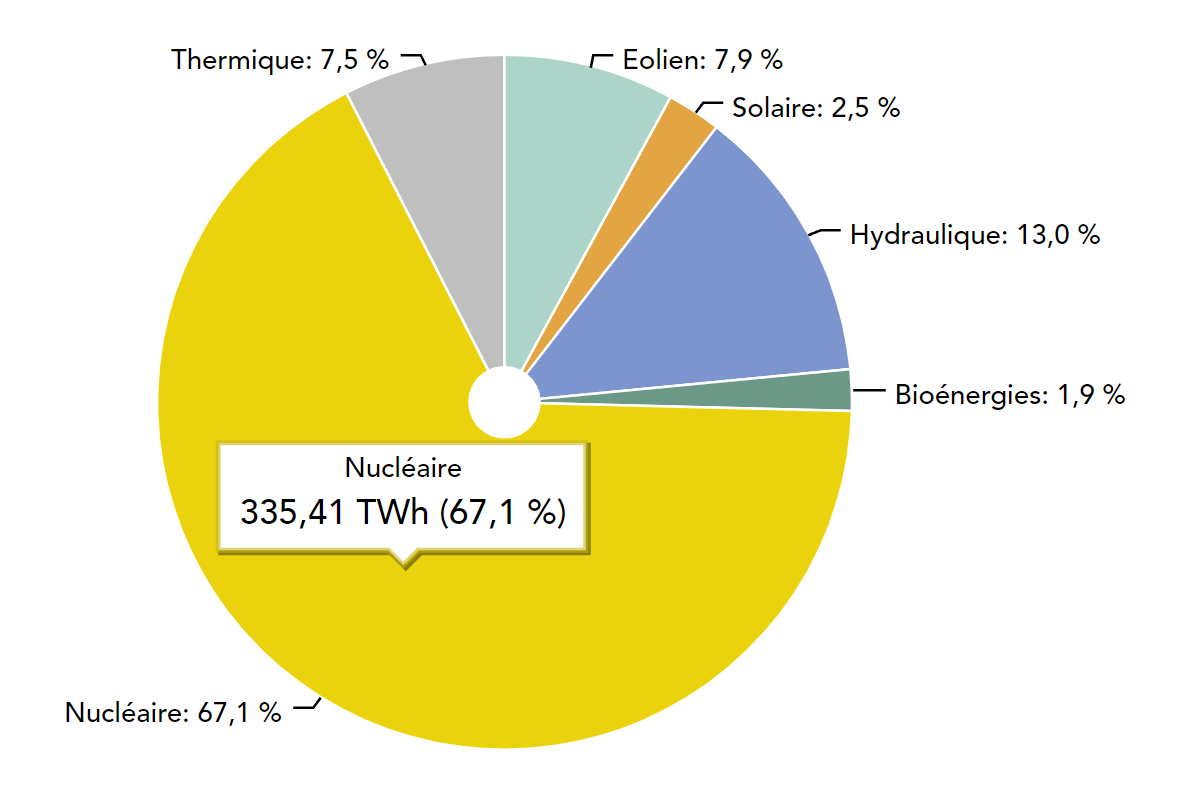
\includegraphics[width=0.6\linewidth]{img/intro/energy_mix.PNG}
\caption{Shared parts of energy production in France. \cite{rte_website} }
\label{fig:france_energy_mix}
\end{figure}

\npar

France accounts for a total of 56 nuclear power plants in 2020, all being Pressurized Water Reactors (PWR). They are dispatched over 19 different geographic locations and split in three electrical power series:

\begin{itemize}
\item 900~MW series (32 plants), launched between 1978 and 1988 (total installed power of 28.8~GW) ;
\item 1300~MW series (20 plants), launched between 1985 and 1994 (total installed power of 26.3~GW) ;
\item N4 series (1450~MW, 4 plants), launched between 2000 and 202 (total installed powed of 6~MW) being the most recent french PWR.
\end{itemize}


%%%%FIGURE OF NUCLEAR POWER PLANTS MAP



\section*{Physical and Technological Background}

\subsection*{Nuclear Energy}

\subsubsection*{Nuclear Fission}

On earth exists only one isotope that is called "fissile" : uranium 235 (noted $^{235}U$). Under certain physical conditions, $^{235}U$ collision with a neutron results in its break-up in two lighter atoms while releasing a total of two to three neutrons and an energy of the order of 200~MeV ($\approx 3.2 \times 10^{-11}$\ J). This amount of energy results from the mass difference between the $^{235}U$ and the products of the fission (atoms and neutrons), which is transferred as kinetic energy to the latter (Figure \ref{fig:fission}).



\begin{figure}[!h]
\centering
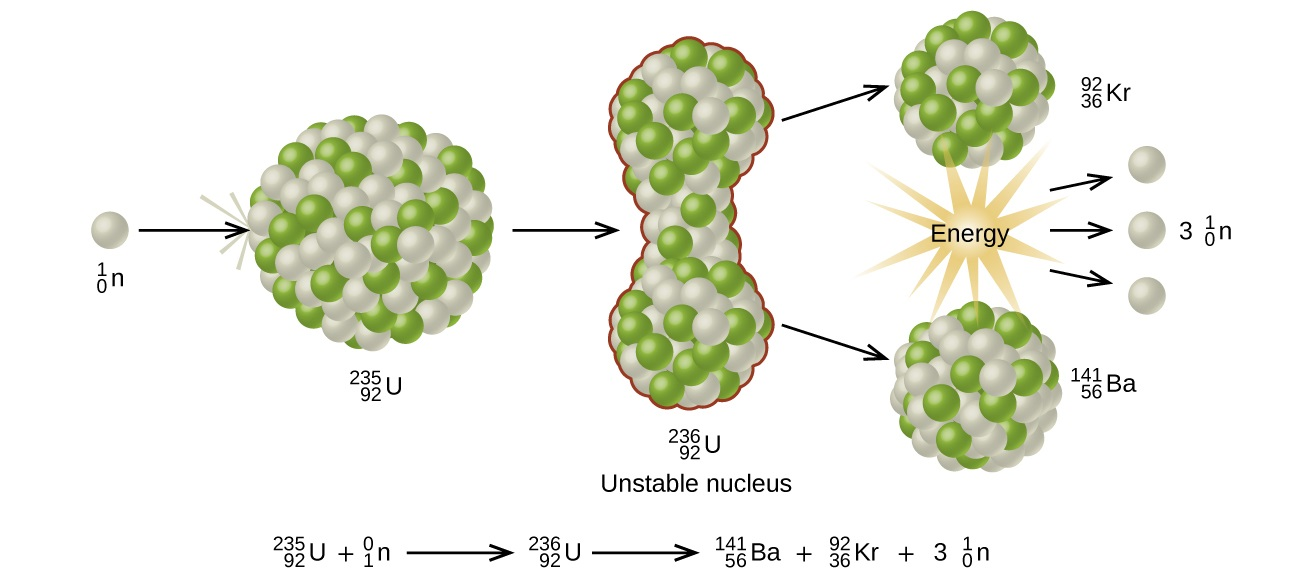
\includegraphics[width=0.6\linewidth]{img/intro/fission.jpg}
\caption{Sketch of the nuclear fission process. \cite{chem_libretext }}
\label{fig:fission}
\end{figure}


$^{235}U$ used in PWR is an isotope of uranium and accounts for only 0.7\% of the common uranium found in nature, most of which being uranium 238 ($^{238}U$) that is not fissile. For nuclear power production, common uranium must be enriched in $^{238}U$ up to 3\% to 5\%.

\subsubsection*{Nuclear Chain Reaction and Energy Production}


Fission presents particular interest for energy production due to its capacity to create a "nuclear chain reaction". Indeed, as multiple neutrons are expelled after the nuclear fission (Figure \ref{fig:fission}), each of them can potentially become a trigger for a new fission of a nearby $^{235}U$ atom. Since each fission releases more neutrons than required for its own triggering, this results in an exponentially increasing number of fission called a nuclear chain reaction.

\npar

However, neutrons actually released by the fission can't directly trigger a new one. They are emitted with a kinetic energy of approximately 2~MeV at which the probability of impacting an other $^{235}U$ is too low to start the nuclear chain reaction. Therefore, a so-called "moderator" is needed to slow down the neutrons through collisions with other atoms. Then the fission reactions lead the nuclear fuel to heat up rapidly and thus needs to be cooled to evacuate the produced energy. Using a fluid, it must both act as a coolant and allow the nuclear chain reaction to continue (moderator role). In french PWR, this is achieved using water as cooling fluid which also moderates the neutrons going through it.

\begin{note*}{}
Other nuclear reactor technologies exist with different fluid such as gas-cooled reactor using graphite as moderator material and carbon dioxyde as coolant.
\end{note*}

\npar

Following the heat exchange between the nuclear fuel and the water, the thermal energy stored in it can be used in a thermodynamic cycle (\eg Hirne cycle) to produce electrical power.



\subsection*{PWR Structure and Operation}

Pressurized Water Reactors are the only type of nuclear power plants operated in France for electricity production. A simplified sketch of a PWR is presented on Figure \ref{fig:pwr_sketch}.

\begin{figure}[!h]
\centering
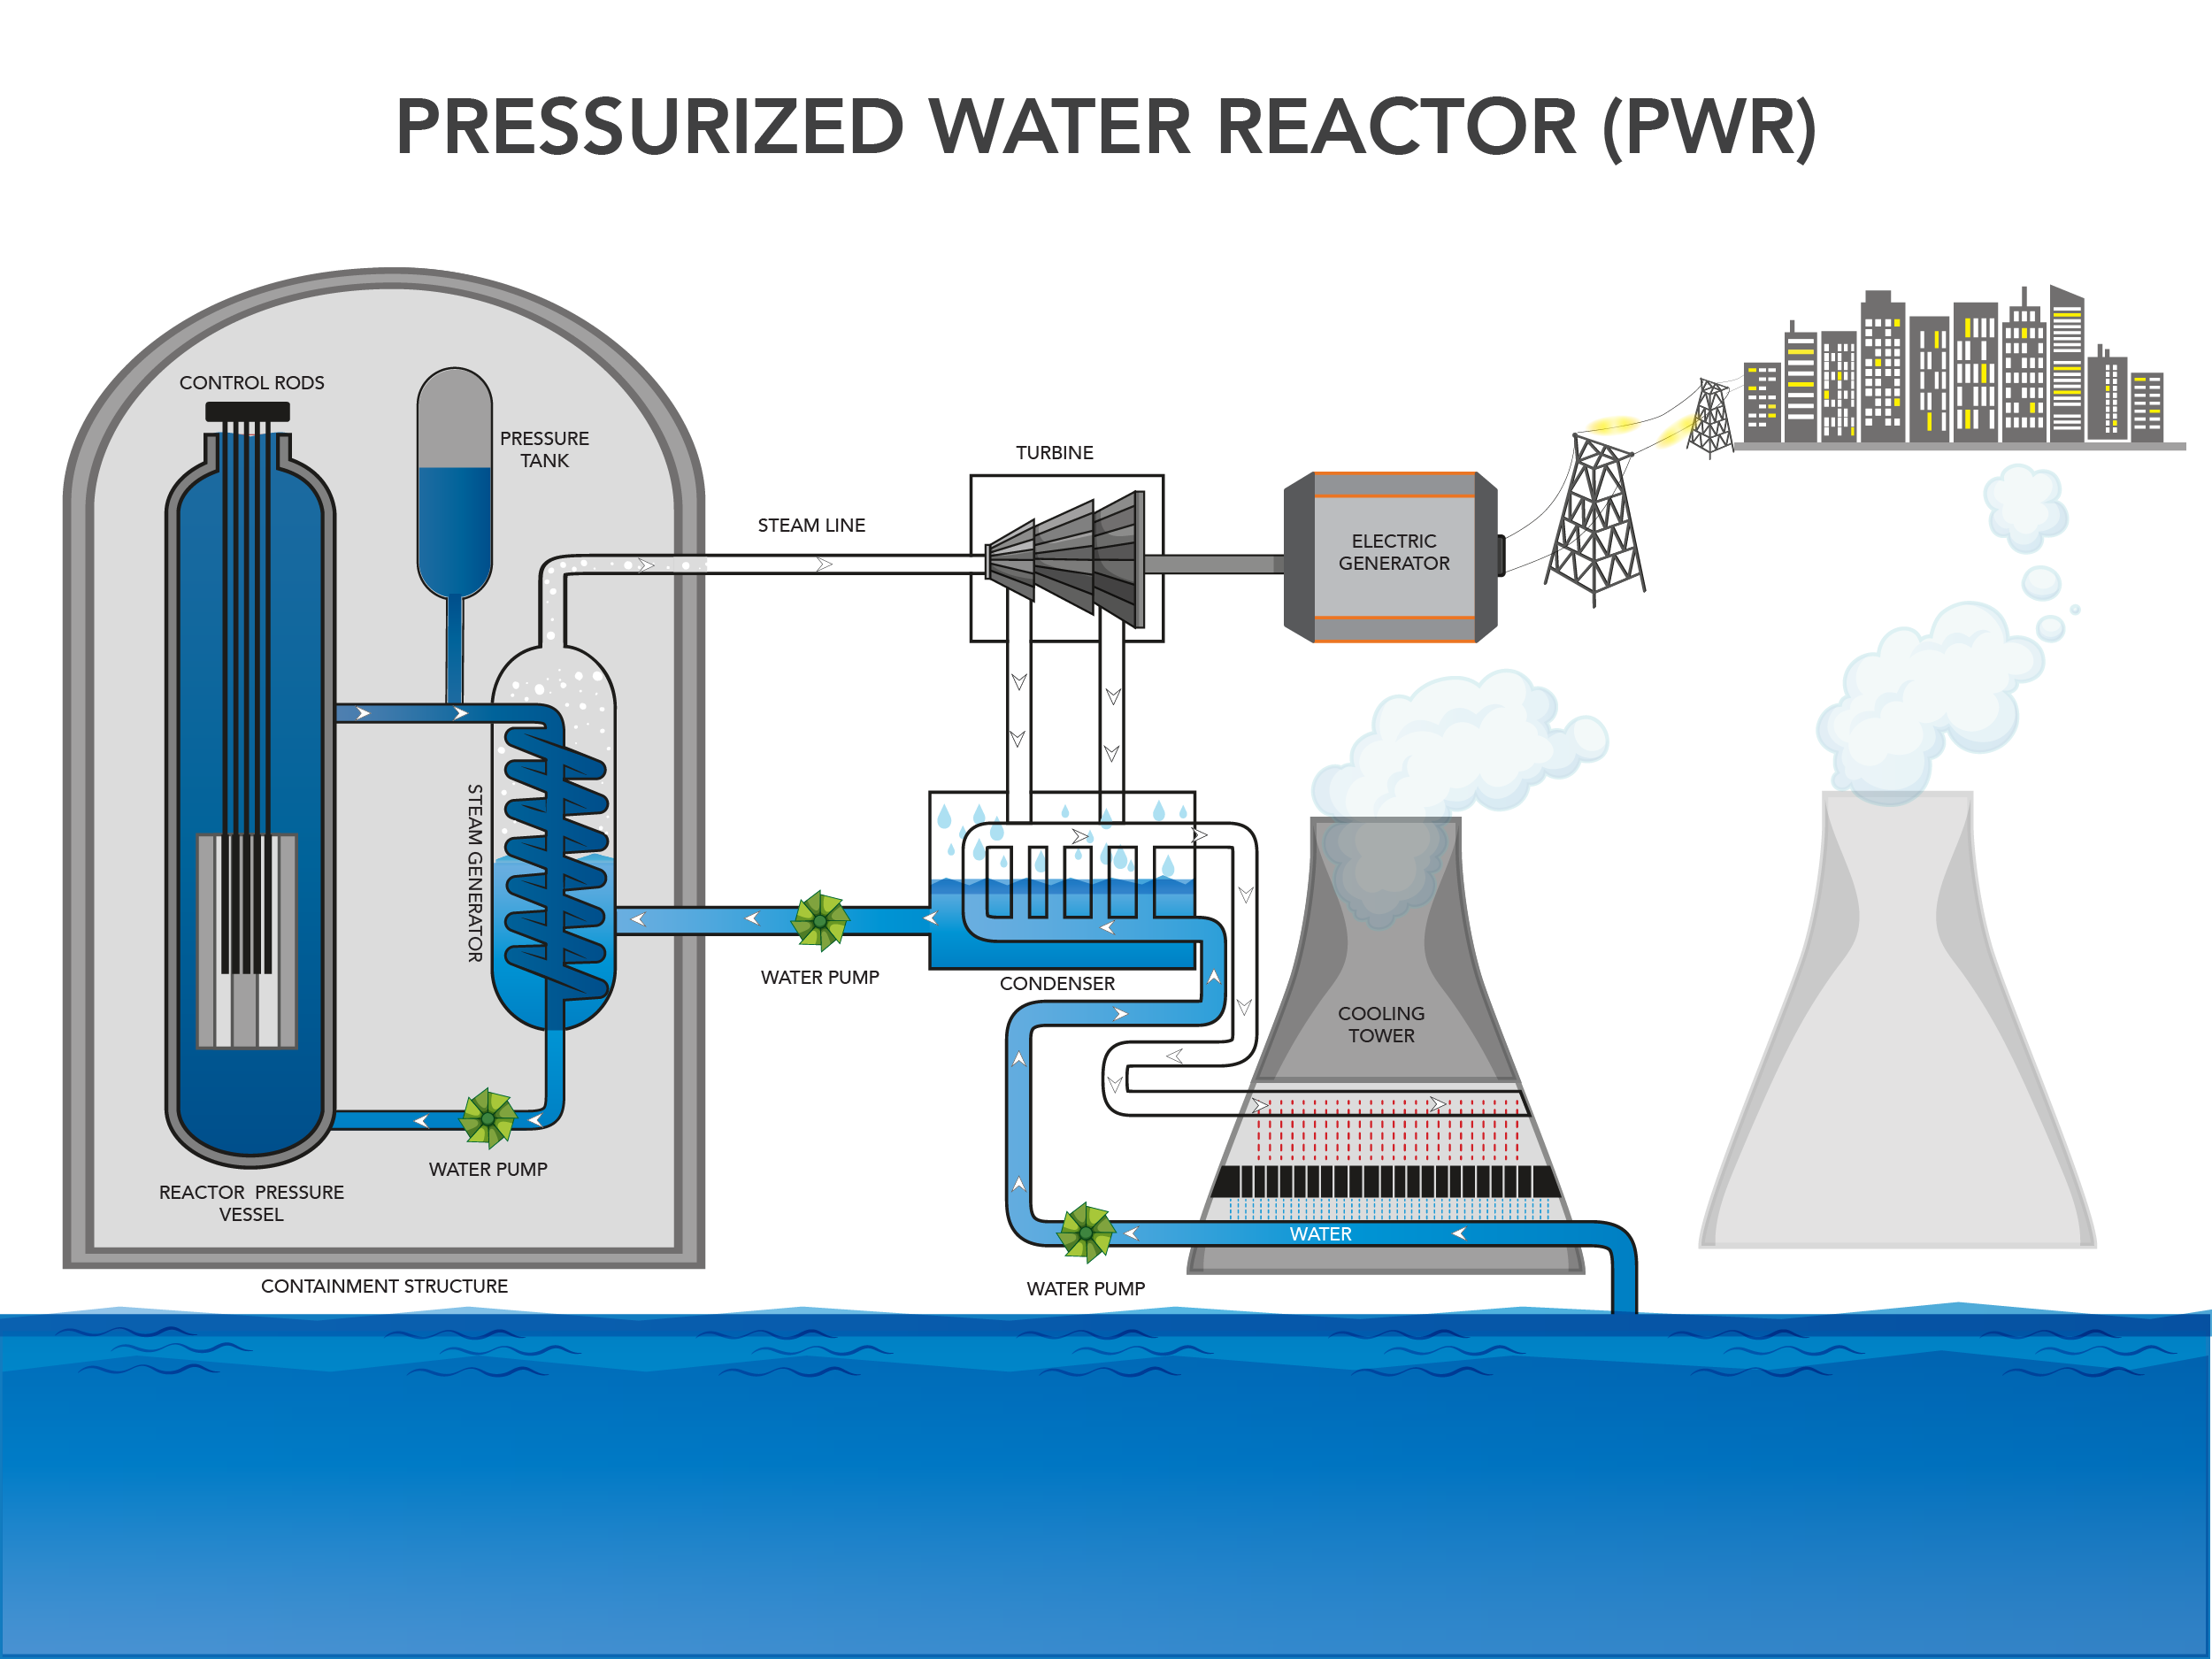
\includegraphics[width=0.7\linewidth]{img/intro/pwr_sketch.png}
\caption{Sketch of a Pressurized Water Reactor \cite{office_nuclear_energy}}
\label{fig:pwr_sketch}
\end{figure}



\subsubsection{Primary Circuit}

The primary circuit aims to collect the thermal energy expelled by the fission reactions within the nuclear fuel rods. The water flowing through the core gathers this energy and transfer it towards the vapor generator, while ensuring a moderating effect to maintain the nuclear chain reaction in the fuel. The primary circuit is fully closed and operates at a pressure close to 155\ bar, a temperature of $300\degC$ and mass flow rates between $3000$ and $5000 \debm$ (approximately 20 tons per second).  


To write :

\begin{itemize}
\item nuclear in france
\item progressive zoom toward the primary circuit and nuclear fuel assembly
\item heat transfer and boiling
\item CHF issue
\item Modeling, component approach, THYC
\item New approaches, CFD, objective of the thesis
\end{itemize}


\part{Modeling and simulation of boiling flows using CFD} % Second part of the thesis

% Chapter 1

\chapter{Presentation of the NEPTUNE\_CFD Code} % Chapter title

\label{chap:ncfd} % For referencing the chapter elsewhere, use \autoref{ch:introduction} 

%----------------------------------------------------------------------------------------

\minitoc


\section{Introduction}

The NEPTUNE\_CFD project (started in 2001) is a research program coordinated by four entities : EDF, CEA, IRSN and Framatome. The initial goals of the project were related to nuclear safety by developing a thermal-hydraulics simulation tool to :

\begin{itemize}
\item Predict the Boiling Crisis in PWR cores ;
\item Study the Loss Of Coolant Accident (LOCA) to predict fuel rod cladding temperature.
\end{itemize}

As a multiphase eulerian code, NEPTUNE\_CFD consists of a local three-dimensional  modeling based on a two fluids-one pressure approach combined with mass, momentum and energy conservation equations for each phase \cite{guelfi_neptune_2007}. 


\npar
%The NEPTUNE\_CFD solver can handle several types of multiphase flows, \eg dispersed vapor-liquid flow of a same component, mixed gas-liquid-solid particles flow of different components, or multiple forms of a single component (dispersed vapor/continuous liquid, dispersed liquid/continuous vapor, continuous liquid/continuous vapor, etc.).
The constitutive equations are solved using a pressure correction and is based on a finite-volume discretization along with a collocated arrangement of the variables. Moreover, NEPTUNE\_CFD allows the use of all type of meshes (hexahedral, tetrahedral, pyramids, etc.), even non-conforming ones, thanks to its face-based data structure. Finally, the code is well-suited for parallel computing, widening its computing capacity to very large meshes.

\npar

The simulations presented in this thesis have all been conducted using the NEPTUNE\_CFD 7.0 modeling framework for dispersed bubbly flows. In the next sections, we will detail the constitutive equations and physical modeling of the code for the simulation of boiling bubbly flows.


\section{Governing Equations for Turbulent Boiling Bubbly Flows}

To simulate two-phase dispersed boiling flows, NEPTUNE\_CFD solves the ensemble-averaged equations of mass conservation, momentum balance and energy conservation for each phase (see Ishii \cite{ishii_thermo-fluid_2011} for details on the derivation).
%As a reminder, the ensemble-averaging of a physical quantity $F_{k}$ for any phase $k$ in a multiphase flows is defined as:



\subsection{Mass Conservation}
\begin{equation}
%MASS
	\dtime{\alpha_{k}\rho_{k}} + \divg{\alpha_{k}\rho_{k} \vect{U_{k}}} = \orangemath{\Gamma_{k}}
	\label{eq:mass}
\end{equation}

Where $\alpha_{k}$, $\rho_{k}$, $\vect{U_{k}}$ are the volumetric fraction, average density and velocity of phase $k$ ; $\orangemath{\Gamma_{k}}=\Gamma_{k,i}+\Gamma_{k,w}$ the interfacial mass transfer term per unit of volume and time split between bulk and wall contribution.
Subscripts $k= L$ or $V$ denotes the liquid or vapor phase, $i$ the interfacial quantities and $w$ the wall contribution.

\subsection{Momentum Balance}

\begin{equation}
%MOMENTUM
	\dtime{\alpha_{k}\rho_{k}\vect{U_{k}}} + \vecdivg{\alpha_{k}\rho_{k} \vect{U_{k}}\otimes \vect{U_{k}}} = -\alpha_{k}\grad{P} + \orangemath{\vect{F_{k,i}}} + \orangemath{\Gamma_{k}}\vect{U_{k,i}} + \alpha_{k}\rho_{k}\vect{g} + \vecdivg{\alpha_{k} \parth{ \tens{\tau_{k,m}} + \orangemath{\tens{\tau_{k,T}}} }}
\label{eq:momentum}
\end{equation}

Where $P$ is the pressure, $\vect{g}$ the gravity, $\orangemath{ \vect{F_{k,i}} }$ the interfacial forces accounting for momentum transfer between phases per unit of volume and time, $\vect{U_{k,i}}$ the interfacial velocity, $\tens{\tau_{k,m}}$ and $\orangemath{ \tens{\tau_{k,T}} }$ respectively the viscous and turbulent (or Reynolds) stress tensor. Subscript $m$ and $T$ respectively denote the molecular (or laminar) and turbulent terms.


\subsection{Energy Conservation}

\begin{equation}
\begin{aligned}
%ENERGY
	\dtime{\alpha_{k}\rho_{k} H_{k}} + \divg{\alpha_{k}\rho_{k} H_{k}\vect{U_{k}}} =& \dtime{\alpha_{k}P} + \orangemath{\Gamma_{k}}H_{k,i}+\orangemath{\vect{F_{k,i}}}\cdot \vect{U_{k}} + \orangemath{Q_{k,I}} + \divg{\alpha_{k}\parth{ \tens{\tau_{k}} + \orangemath{\tens{\tau_{k,T}}} }\cdot \vect{U_{k}}}\\
	& + \divg{\alpha_{k} \parth{-\parth{ \lambda_{k,m}+\orangemath{\lambda_{k,T}}}\grad{T_{k}}}} + \alpha_{k}\rho_{k}\vect{g}\cdot \vect{U_{k}} + \orangemath{Q_{k,w}}
\end{aligned}
\label{eq:energy}
\end{equation}

Where $H_{k}=e_{k}+\dfrac{U_{k}^{2}}{2}+\dfrac{P}{\rho_{k}}=h_{k}+\dfrac{U_{k}^{2}}{2}$ is the total enthalpy of phase $k$, $H_{k,i}$ the interfacial-averaged enthalpy, $\orangemath{ Q_{k,i} }$ the interfacial heat flux per unit of volume and time, $\lambda_{k,m}$ and $\orangemath{ \lambda_{k,T} }$ respectively being the laminar and turbulent thermal conductivity, $T_{k}$ the temperature, $\orangemath{ Q_{k,w} }$ the heat flux from the wall to phase $k$ per unit of volume and time.

\npar

The viscous and Reynolds stress tensors read:

\begin{align}
\tens{\tau_{k,m}} &= \mu_{k} \parth{ \vecgrad{\vect{U_{k}}}+\vecgrad{U_{k}}^{T}  - \frac{2}{3}\divg{\vect{U_{k}}}\tens{I} }\\
\parth{\orangemath{\tens{\tau_{k,T}}} }_{i,j} &= -\rho_{k} \left< U'_{k,i}U'_{k,j} \right>_{k}
\end{align}
with $\vect{U'_{k}}$ is the fluctuating part of velocity for phase $k$.


\npar

This ensemble-average approach requires a given number of closure laws since this mathematical averaging operation removes most of the information about smaller scales physics (compared to the mesh size) such as interfacial exchanges between phases or wall-fluid interaction. Terms for which this modeling effort is needed are colored in orange in equations \ref{eq:mass}, \ref{eq:momentum} and \ref{eq:energy}. Following sections detail the physical modeling for each of those terms. 


\section{Interfacial Transfers Closure Laws}
\label{sec:int_transfers}

The interfacial transfers of mass, momentum and energy are respectively noted in equations \ref{eq:mass}, \ref{eq:momentum} and \ref{eq:energy} : $\Gamma_{k}$, $\vect{F_{k,i}}$ and $Q_{k,i}$.

\subsection{Heat and Mass Transfers}
\label{subsec:ncfd_interf_mass}


The mass transfer term, can be written as: 

\begin{align}
\Gamma_{L,i} + \Gamma_{V,i} = 0\\
%
\Gamma_{L,w} + \Gamma_{V,w} = 0
\end{align}
with $\Gamma_{V,w} \geq 0$ in the case of boiling flows. This finally gives:

\begin{equation}
\Gamma_{L}=-\Gamma_{V}
\end{equation}

\npar
The interfacial heat flux $Q_{k,i}$ can be rewritten in terms of interfacial area concentration $a_{i}$ : 

\begin{equation}
Q_{k,i}=q''_{k,i}a_{i}
\end{equation} 

\npar

Neglecting the mechanical contribution compared to the thermal terms, the energy jump condition can then be expressed as :

\begin{equation}
\sum_{k=L,V}\parth{\Gamma_{k,i}h_{k,i} + q''_{k,i}a_{i}}=0
\label{eq:ncfd_energy_jump}
\end{equation}

The estimation of $h_{k,i}$ is not straightforward since it can either be supposed as:

\begin{enumerate}
\item[H1)] The saturation enthalpy of phase $k$ at the system pressure ;
\item[H2)] The phase-averaged enthalpy.
\end{enumerate}

\npar
In NEPTUNE\_CFD, the assumption H2 is chosen, thus giving the bulk condensation rate :

\begin{equation}
\Gamma_{L,i}=\frac{a_{i}\parth{q''_{L,i}+q''_{V,i}}}{h_{V}-h_{L}}
\label{eq:ncfd_cond_rate}
\end{equation}


The interfacial heat flux densities $q''_{k,i}$ and interfacial area concentration $a_{i}$ are expressed as:

\begin{align}
q''_{k,i}=C_{k,i}\parth{T_{sat}(P)-T_{k}}\\
a_{i}=6 \alpha_{V}/D_{V}
\end{align}
with $D_{V}$ being the vapor phase Sauter mean bubble diameter and $C_{k,i}$ the interfacial heat transfer coefficient.

\npar

\begin{note*}{}
The interfacial area is computed using the transport equation of {Ruyer} \& {Seiler} \cite{ruyer_modelisation_2009} that accounts for bubble breakup and coalescence to estimate bubble diameter.
\end{note*}


\subsubsection{Subcooled Liquid}

For subcooled liquid, the following heat transfer coefficient is used \cite{ranz_evaporation_1952, manon_contribution_2000}:

\begin{align}
C_{L,i}&=\frac{\Nu_{L}\lambda_{L}}{D_{V}}\\
%
Nu_{L}&=2+0.6\Re_{b}^{1/2}\Pr_{L}^{1/3}
\label{eq:ncfd_subcooled_L}
\end{align}

Where $\Re_{b}$ is the bubble Reynolds number $Re_{b}=\dfrac{\norm{\vect{U_{V}}-\vect{U_{L}}}D_{V} }{\nu_{L}}$ and $\Pr_{L}=\dfrac{\nu_{L}}{\eta_{L}}$ the liquid Prandtl number with $\nu_{L}$ and $\eta_{L}$ respectively being the liquid kinematic viscosity and thermal diffusivity.


\subsubsection{Superheated Liquid}

On the other hand, if the liquid is overheated, the maximum of three heat transfer coefficients accounting for different heat transfer mechanisms is taken \cite{berne_analyse_1983}:

\begin{equation}
C_{L,i}=\max{C_{L,i,1}\ ;\ C_{L,i,2}\ ;\ C_{L,i,3}}
\label{eq:ncfd_supheat_L}
\end{equation}

With $C_{L,i,n}=\dfrac{\lambda_{L}\Nu_{L,n}}{D_{V}}$ and :

\begin{equation}
\label{eq:nusselt}
 Nu_{L,1}=2 \text{ ; } Nu_{L,2}=\frac{12}{\pi} \Ja_{L} \text{ ; }  Nu_{L,3}=\sqrt{\frac{4}{\pi}Pe} 
\end{equation}


where $\Pe=\Re_{b} \Pr_{L}$ is the Peclet number, $\Ja_{L}=\dfrac{ \rho_{L}c_{p,L}\bars{T_{sat}-T_{L}}}{\rho_{V} h_{LV}} $ the liquid Jakob number and $h_{LV}$ the latent heat of vaporization. 

\npar

Those three Nusselt numbers respectively correspond to stationary conduction around a sphere, transient conduction for a spherical bubble growth in uniformly superheated liquid \cite{plesset_growth_1954} and transient convection around a sphere in a superheated flow \cite{ruckenstein_mass_1964}.

\subsubsection{Vapor Heat Transfer}

For the vapor phase, a simple law that ensures the vapor temperature to stay close to the saturation temperature is used (which is expected for small bubbles, \eg in a PWR) :

\begin{equation}
C_{V,i}a_{i}=\frac{\alpha_{V}\rho_{V}c_{p,V}}{t_{c}}
\label{eq:ncfd_vap_relaxation}
\end{equation}
where $c_{p,V}$ is the vapor heat capacity at constant pressure and $t_{c}$ a characteristic (relaxation) time given by the user (default value being $t_{c}=0.01\ \text{s}$) .

\subsection{Interfacial Forces}
\label{subsec:ncfd_interf_qdm}

The interfacial momentum transfer (excluding transfer associated to transfer of mass $\Gamma_{k}$) is assumed to be composed of 4 different forces being the, drag $D$, the added mass $AM$, the lift $L$ and the turbulent dispersion $TD$:

\begin{equation}
\vect{F_{k,i}}=\vect{F_{k,D}} + \vect{F_{k,AM}} +\vect{F_{k,L}} +\vect{F_{k,TD}}
\label{eq:ncfd_force_balance}
\end{equation}

\npar

The turbulent dispersion force $\vect{F_{k,TD}}$ originates from the averaging operation conducted on the three other forces expressions, detailed in equations \ref{eq:ncfd_drag}, \ref{eq:ncfd_added_mass}, \ref{eq:ncfd_lift} and \ref{eq:ncfd_turb_disp}.

\subsubsection{Drag Force}

The drag force is modeled according to Ishii \& Zuber \cite{ishii_drag_1979}:

\begin{equation}
\vect{F_{V,D}}=-\vect{F_{L,D}}=-\frac{1}{8}a_{i}\rho_{L}C_{D}\norm{ \vect{U_{V}}-\vect{U_{L}} }\parth{\vect{U_{V}}-\vect{U_{L}} }
\label{eq:ncfd_drag}
\end{equation}

\begin{equation}
C_{D} = \frac{2}{3}D_{V}\sqrt{\dfrac{g\parth{\rho_{L}-\rho_{V}}}{\sigma}}\parth{ \frac{1 + 17.67~f\parth{\alpha}^{1.67}}{18.67f\parth{\alpha}} }, \ f\parth{\alpha} = \parth{1-\alpha}^{1.5}\ \text{for distorted bubbles.}
\end{equation}

\begin{equation}
C_{D} = \frac{8}{3} \parth{1-\alpha}^{2}\ \text{for churn-turbulent regime.}
\end{equation}

\subsubsection{Added Mass Force}

The added mass force is modeled  following Zuber \cite{zuber_dispersed_1964}:

\begin{align}
\vect{F_{V,AM}}=-\vect{F_{L,AM}}=&-C_{AM} \frac{1+2\alpha_{V}}{1-\alpha_{V}}\alpha_{V}\rho_{L}\\
&\times \crocht{ \parth{\dtime{\vect{U_{V}}}+\vecgrad{\vect{U_{V}}}\cdot \vect{U_{V}} } - \parth{\dtime{\vect{U_{L}}}+\vecgrad{\vect{U_{L}}}\cdot \vect{U_{L}} } }
\label{eq:ncfd_added_mass}
\end{align}
with $C_{AM}=\dfrac{1}{2}$ and the term $\dfrac{1+2\alpha_{V}}{1-\alpha_{V}}$ accounts for the impact of bubble concentration.

\subsubsection{Lift Force}

The lift force is modeled based on the experiments of Tomiyama \etal \cite{tomiyama_transverse_2002}:

\begin{equation}
\vect{F_{V,L}}=-\vect{F_{L,L}}=-C_{L}\alpha_{V}\rho_{L}\parth{\vect{U_{V}}-\vect{U_{L}} }\wedge \parth{\rot{\vect{U_{L}}} }
\label{eq:ncfd_lift}
\end{equation}

\begin{equation}
C_{L} = \begin{cases}
    \min{0.288\tanh{0.121\Re_{b}}\ ;\ 0.00105 \Eo_{H}^{3}-0.0159\Eo_{H}^{2} - 0.0204\Eo_{H}+0.474}, & \text{if}\ \Eo_{H}<4\\
   0.00105 \Eo_{H}^{3}-0.0159\Eo_{H}^{2} - 0.0204\Eo_{H}+0.474, & \text{if}\ 4\leq \Eo_{H} \leq 10\\
   -0.27, & \text{if}\ \Eo_{H}>10
  \end{cases}
\end{equation}
where $\Eo_{H} = \dfrac{g\parth{\rho_{V}-\rho_{L}}D_{H}^{2}}{\sigma}$ is a modified E\"otv\"os number with:

\begin{equation}
D_{H} = D_{V}\sqrt[3]{1+0.163^Eo^{0.757}}
\end{equation}

\subsubsection{Turbulent Dispersion Force}

The turbulent dispersion force is computed following the General Turbulent Dispersion approach presented by Lavieville \etal \cite{lavieville_generalized_2017}:

\begin{equation}
\vect{F_{V,TD}}=-\vect{F_{L,TD}}=-\frac{2}{3}\alpha_{L}\alpha_{V}C_{TD}\grad{\alpha_{V}}
\label{eq:ncfd_turb_disp}
\end{equation}

The value of $C_{TD}$ notably depends on the fluid turbulence, drag force, added mass force. Further details on its derivation are presented in Lavieville \etal \cite{lavieville_generalized_2017}.

%\begin{align}
%C_{TD} = \frac{F_{12}\tau_{12}^{t}}{3\rho_{L}} \frac{b+\eta_{r}}{1+\eta_{r}} + \frac{C_{12}}{\rho_{L}}\frac{b^{2} + \eta_{r}}{1+\eta_{r}} - \frac{b+\eta_{r}}{1+\eta_{r}} - \frac{\alpha_{L}}{\alpha_{V}}
%\label{eq:ncfd_CTD}\\
%%
%b&= \frac{1+C_{VM}}{\frac{\rho_{L}}{\rho_{V}} + C_{VM}}
%\end{align}

%with $C_{D}$, $C_{AM}$, $C_{L}$ and $C_{TD}$ the associated forces coefficients, respectively taken from \textsc{Ishii}\cite{ishii1967}, \textsc{Zuber}\cite{zuber1964}, \textsc{Tomiyama}\cite{tomiyama2002} and the Generalized Turbulent Dispersion model (GTD) from \textsc{Lavieville} \etal \cite{lavieville2017}.

\section{Turbulence Modeling}
\label{subsec:turbulence}

%\begin{equation}
%\dtime{R_{ij}} + U_{k}
%\end{equation}
%
%\begin{equation}
%\dtime{\tens{R}} + \vect{U_{k}}\cdot \grad{R_{ij}} = 
%\end{equation}

For bubbly flow simulations, only liquid phase turbulence is taken into account while it is neglected for the vapor phase. The prescribed model is the Reynolds Stress Model $R_{ij}-\varepsilon~SSG$ from Speziale, Sarkar and Gatski \cite{speziale_modelling_1991} adapted to two-phase boiling flows by Mimouni \etal\cite{mimouni_combined_2011}. Noting $R_{ij} = \left< U'_{L,i}U'_{L,j} \right>_{L}$ and $\alpha = \alpha_{V}$, it reads:

\begin{align}
\parth{1-\alpha}+\frac{\mathrm{D}\rho_{L}R_{ij}}{\mathrm{D}t}  = & \frac{\partial}{\partial x_{k}}\crocht{ \parth{\rho_{L}\nu_{L} + \rho_{L}C_{s} \frac{k}{\varepsilon}R_{ij}} \frac{\partial}{\partial x_{k}}\parth{ \parth{1-\alpha} R_{ij} } } \\
&+ \parth{1 - \alpha}\parth{P_{ij} + G_{ij} + \Phi_{ij} + \varepsilon_{ij}}
\end{align}
where $\mathrm{D}/\mathrm{D}t$ is the Lagrangian derivative, $k$ the turbulent kinetic energy, $\varepsilon$ the turbulent pseudo-dissipation rate, $\tens{P}$ the turbulent production term, $\tens{G}$ the work of gravity force, $\tens{\Phi}$ the pressure-strain term and $\tens{\varepsilon}$ the viscous dissipation.

\npar

All those terms need a proper modeling, for which we refer the reader to Mimouni \etal \cite{mimouni_combined_2011}.

\npar

The transport equation on $\varepsilon$ also includes the impact of $\alpha$:


\begin{align}
\parth{1-\alpha}+\frac{\mathrm{D}\varepsilon}{\mathrm{D}t}  &= \frac{\partial}{\partial x_{k}}\crocht{ C_{\varepsilon} \frac{k}{\varepsilon}\left< U'_{L,k}U'_{L,l} \right>_{L}  \frac{\partial \parth{1-\alpha} \epsilon}{\partial x_{l}} } \\
&+ \parth{C_{\varepsilon_{1}} + C_{\varepsilon_{3}}G + C_{\varepsilon_{4}}k\frac{\partial U_{L,k}}{\partial x_{k}} - C_{\varepsilon_{2}}\epsilon } \frac{\parth{1-\alpha}\epsilon}{k}
\end{align}

\npar

We conclude by specifying the values used for the constants in NEPTUNE\_CFD (Table \ref{tab:ncfd_ssg_constants}).


\begin{table}[!h]
\centering
\begin{tabular}{c c c c c c c c c c} 
\hline
$C_{s}$ & $C_{1}$ & $C_{2}$ & $C_{1}^{\omega}$ & $C_{2}^{\omega}$ & $C_{\varepsilon}$ & $C_{\varepsilon_{1}}$ & $C_{\varepsilon_{2}}$ & $C_{\varepsilon_{3}}$ & $C_{\varepsilon_{4}}$ \\
\hline
0.2 & 1.8 & 0.6 & 0.5 & 0.3 & 0.18 & 1.44 & 1.92 & 1.44 & 0.33\\
\hline
\end{tabular}

\caption{Constant values for the SSG model in NEPTUNE\_CFD}
\label{tab:ncfd_ssg_constants}

\end{table}




\section{Wall Boiling Model}
\label{sec:ncfd_HFP}

The modeling of the heterogeneous boiling phenomenon at the wall is based on a Heat Flux Partitioning (HFP) model,  from Kurul \& Podowski original work\cite{kurul_multidimensional_1990} who divided the wall heat flux density $\phi_{w}$ in three terms  :

\begin{itemize}
\item A single phase convective heat flux $\phi_{c,L}$ heating the liquid through the fraction of the wall area unaffected by the vapor bubbles ;
\item A vaporization heat flux $\phi_{e}$ which accounts for the generation of vapor through heterogeneous nucleation ;
\item A quenching heat flux $\phi_{q}$ to represent the thermal impact of bubbles departing from the wall and being replaced by cool liquid
\end{itemize}

A fourth flux is added to this HFP in NEPTUNE\_CFD, following Mimouni \etal\cite{mimouni_computational_2016} who consider a convective heat flux towards the vapor $\phi_{c,V}$ when the wall area is covered by a dense accumulation of bubbles. 

\npar

The model is then ponderated by a phenomenological function $f_{\alpha_{L}}$ enhancing $\phi_{c,V}$ when the void fraction at the wall becomes large. It thus gives Equation \ref{eq:ncfd_HFP} :

\begin{equation}
\phi_{w}=f_{\alpha_{L}} \parth{\phi_{c,L}+\phi_{e}+\phi_{q}} + \parth{1+f_{\alpha_{L}} }\phi_{c,V}
\label{eq:ncfd_HFP}
\end{equation}
where $f_{\alpha_{L}}$ verifies smooth conditions $\lim\limits_{\alpha_{L} \to 1} f_{\alpha_{L}} = 1$, $\lim\limits_{\alpha_{L} \to 0} f_{\alpha_{L}} = 0$, $\lim\limits_{\alpha_{L} \to 0} \dfrac{f_{\alpha_{L}} }{ \alpha_{L}} = 0$ and $\lim\limits_{\alpha_{L} \to 1} \dfrac{ 1 - f_{\alpha_{L}} }{ 1 - \alpha_{L}} = 0$.

\npar
The convective heat fluxes are expressed as:

\begin{align}
\phi_{c,k} &=A_{k}h_{k,log}\parth{T_{w}-T_{k}}\\
%
h_{k,log} &=\frac{ \rho_{k}c_{p,k}{U_{\tau}}}{{T_{L}^{+}} }
\label{eq:ncfd_hfc}
\end{align}
where $A_{k}$ the fraction of the wall area facing phase $k$, $T_{w}$ the wall temperature and $h_{k,log}$ the wall logarithmic convective heat transfer coefficient to phase $k$ based on the wall functions for friction velocity $U_{\tau}$ and non-dimensional liquid temperature $T_{L}^{+}$ described in \ref{subsec:wall_func}.

\npar
The vaporization heat flux is computed following:

\begin{equation}
\phi_{e}=N_{sit}f\rho_{V}h_{LV}\frac{\pi D_{d}^{2}}{6}
\label{eq:phie_NCFD}
\end{equation}


Closure of physical parameters needed are :

\begin{itemize}
\item $N_{sit}$ the nucleation site density modeled as \cite{lemmert_influence_1977}:
\begin{equation}
N_{sit}=\crocht{210\parth{T_{w}-T_{sat}} }^{1.8}
\label{eq:nsit_NCFD}
\end{equation}

\item $f$ the bubble detachment frequency expressed as \cite{cole_bubble_1967}: 
\begin{equation}
f=\sqrt{\frac{4}{3}\frac{g\bars{\rho_{V}-\rho_{L}} }{\rho_{L}D_{d}}}
\end{equation}

\item $D_{d}$ the bubble detachment diameter given by \"Unal correlation \cite{unal_maximum_1976} corrected by Bor\'ee \etal \cite{boree_ecoulements_1992} (Equation \ref{eq:ncfd_unal_boree}).

\end{itemize}



\begin{align}
D_{d}&=2.42\times 10^{-5} P^{0.709} \frac{a}{\sqrt{b\varphi}}\text{ with }
  \label{eq:ncfd_unal_boree}\\
  %
 a&=\frac{\parth{T_{w}-T_{sat}} \lambda_{w}}{2\rho_{V}h_{LV}\sqrt{\pi\eta_{w}}}\\
 %
  b&=\begin{cases}
    \dfrac{T_{sat}-T_{L}}{2 \parth{1-\dfrac{\rho_{V}}{\rho_{L}} }}, & \text{if $St\leq0.0065$}\\
    \dfrac{1}{2 \parth{1-\rho_{V}/\rho_{L} })}\dfrac{\phi_{c,L}+\phi_{e}+\phi_{q}}{0.0065\rho_{L}c_{p,L}\norm{\vect{U_{L}}}}, & \text{\text{if $St>0.0065$}}
    \end{cases}
\end{align}
where $\lambda_{w}$ and $\eta_{w}$ are the wall thermal conductivity and diffusivity, $St=\dfrac{\phi_{c,L}+\phi_{e}+\phi_{q}}{\rho_{L}c_{p,L}\norm{\vect{U_{L}}}\parth{T_{sat}-T_{L} }}$ is the Stanton number and $\varphi=\displaystyle \max{1 ; \parth{\frac{\norm{\vect{U_{L}}}}{U_{0}} }^{0.47} }$ with $U_{0}=0.61\text{m/s}$

\npar

Finally, the quenching heat flux follows the approach of {Del Valle} \& {Kenning} \cite{del_valle_subcooled_1985} supposing that it follows a semi-infinite transient conduction regime: 

\begin{equation}
\phi_{q}=A_{q}t_{q}f\frac{2\lambda_{L} \parth{T_{w}-T_{L}}}{\sqrt{\pi \eta_{L}t_{q}}}
\label{eq:ncfd_phiq}
\end{equation} 
where $t_{q}$ is the quenching time, supposed to be equal to $1/f$, and $A_{q}=N_{sit} \pi R^{2}$ the area experiencing quenching.



\section{Wall Function for Dispersed Boiling Flows}
\label{subsec:wall_func}

In boiling flows, the formation of bubbles at the wall may disturb the liquid velocity profile in the boundary layer. To take this phenomena into account, Mimouni \etal\cite{mimouni_computational_2016} proposed a wall function for boiling flows which tends to the single-phase formulation when $\alpha_{V} \rightarrow 0$ and depends on the bubble diameter and density at the wall: 

\begin{equation}
U^{+}=\frac{1}{\kappa}\ln{ y^{+} } + B - \Delta U^{+} \text{ with } 
\label{eq:ncfd_wall_law}
\end{equation}
where $\kappa$=0.41 is the Von Karman constant, $B=5.3$ the standard single-phase logarithmic law constant and $\Delta U^{+}$ represents the offset of $U^{+}$ due to the wall roughness induced by the presence of bubble.

\npar

The correction $\Delta u^{+}$ is computed as:

\begin{align}
  \Delta U^{+}&=\begin{cases}
    0 & \text{if $k_{r}^{+}\leq 11.3$}\\
    \dfrac{1}{\kappa}\ln{ 1+ C_{kr}k_{r}^{+} } & \text{\text{if $k_{r}^{+}>11.3$}}
  \end{cases} \\
%
k_{r}^{+}&= \dfrac{k_{r}\sqrt{U_{\tau}U_{T}}}{\nu_{L}} \\
%
k_{r}&=\alpha_{V}d_{V}\\
%
U_{T}&=C_{\mu}^{1/4}\sqrt{k_{L}}
\end{align}
with $C_{kr}=0.5$ , $k_{r}$ a "bubble roughness Reynolds number", $C_{\mu}=0.09$ defined from the $k-\varepsilon$ and $k_{L}$ the liquid turbulent kinetic energy.

\npar

The non-dimensional wall liquid temperature $T_{L}^{+}$ is modeled according following a Van Driest formulation:

\begin{equation}
T_{L}^{+} = \int_{0}^{y^{+}} \frac{2\mathrm{d}y}{1 + \dfrac{1}{2}\dfrac{\Pr_{L}}{\Pr_{T}}\sqrt{1+4\kappa^{2} {y^{+}}^{2}  \parth{1-\exp{-y^{+}/A}}^{2}}}
\end{equation}
with $A=25.6$, $\Pr_{T} = 0.9$ and $y^{+} \approx 100$ usually.

\section{Conclusions}

In this chapter, we presented the constitutive equations of NEPTUNE\_CFD. As a summary, the main features of the modeling for dispersed bubbly flows are:

\begin{itemize}
\item Conservation equation for mass, momentum and energy are solved for liquid and vapor ;
\item Interfacial momentum transfer is modeled by including different forces, with in particular recent formulations for turbulent dispersion and lift ;
\item Turbulence is modeled by accounting for vapor presence in the $R_{ij}-\varepsilon$ SSG model along with a wall law based on local bubble size ;
\item Wall boiling is based on a Heat Flux Partitioning approach extending the original formulation of Kurul \& Podowski \cite{kurul_multidimensional_1990} by accounting for vapor convection at high wall void fraction.
\end{itemize}

In order to assess this modeling framework, we will further perform simulations using NEPTUNE\_CFD. In next Chapter, we present the DEBORA database that will serve as validation reference in Chapter \ref{chap:debora_ncfd}.


%\begin{equation}
%\label{eq:wall_law} 
%  T_{L}^{+}=\begin{cases}
%    Pr_{L}~y^{+}, & \text{if $y^{+}\leq 13.2$}\\
%    8.67Pr_{L,T}\parth{ \frac{Pr_{L}}{Pr_{L,T}}-1 } \parth{\frac{Pr_{L,T}}{Pr_{L}} }^{0.25} + \frac{Pr_{L,T}}{\kappa}\ln{Ey^{+}}  & \text{\text{if $y^{+}>13.2$}}
%  \end{cases}
%\end{equation}
%
%With $Pr_{L,T}=0.9$ the turbulent liquid Prandtl number, and $E=7.76$ a constant for smoth walls. % Cha pter NCFD
%% Chapter 3

\chapter{Math Test Chapter} % Chapter title

\label{ch:mathtest} % For referencing the chapter elsewhere, use \autoref{ch:mathtest}

%----------------------------------------------------------------------------------------

\lipsum[13]

%----------------------------------------------------------------------------------------

\section{Some Formulas}

Due to the statistical nature of ionisation energy loss, large fluctuations can occur in the amount of energy deposited by a particle traversing an absorber element\footnote{Examples taken from Walter Schmidt's great gallery: \\ \url{http://home.vrweb.de/~was/mathfonts.html}}.  Continuous processes such as multiple scattering and energy loss play a relevant role in the longitudinal and lateral development of electromagnetic and hadronic showers, and in the case of sampling calorimeters the measured resolution can be significantly affected by such fluctuations in their active layers.  The description of ionisation fluctuations is characterised by the significance parameter $\kappa$, which is proportional to the ratio of mean energy loss to the maximum allowed energy transfer in a single collision with an atomic electron: \graffito{You might get unexpected results using math in chapter or section heads. Consider the \texttt{pdfspacing} option.}
\begin{equation}
\kappa =\frac{\xi}{E_{\mathrm{max}}} %\mathbb{ZNR}
\end{equation}
$E_{\mathrm{max}}$ is the maximum transferable energy in a single collision with an atomic electron.
\[E_{\mathrm{max}} =\frac{2 m_{\mathrm{e}} \beta^2\gamma^2 }{1 + 2\gamma m_{\mathrm{e}}/m_{\mathrm{x}} + \left ( m_{\mathrm{e}} /m_{\mathrm{x}}\right)^2}\ ,\]
where $\gamma = E/m_{\mathrm{x}}$, $E$ is energy and $m_{\mathrm{x}}$ the mass of the incident particle, $\beta^2 = 1 - 1/\gamma^2$ and $m_{\mathrm{e}}$ is the electron mass. $\xi$ comes from the Rutherford scattering cross section and is defined as:
\begin{eqnarray*} \xi  = \frac{2\pi z^2 e^4 N_{\mathrm{Av}} Z \rho
\delta x}{m_{\mathrm{e}} \beta^2 c^2 A} =  153.4 \frac{z^2}{\beta^2}
\frac{Z}{A}
\rho \delta x \quad\mathrm{keV},
\end{eqnarray*}
where

\begin{tabular}{ll}
$z$ & charge of the incident particle \\
$N_{\mathrm{Av}}$ & Avogadro's number \\
$Z$ & atomic number of the material \\
$A$ & atomic weight of the material \\
$\rho$ & density \\
$ \delta x$ & thickness of the material \\
\end{tabular}

$\kappa$ measures the contribution of the collisions with energy transfer close to $E_{\mathrm{max}}$.  For a given absorber, $\kappa$ tends towards large values if $\delta x$ is large and/or if $\beta$ is small.  Likewise, $\kappa$ tends towards zero if $\delta x $ is small and/or if $\beta$ approaches $1$.

The value of $\kappa$ distinguishes two regimes which occur in the description of ionisation fluctuations:

\begin{enumerate}
\item A large number of collisions involving the loss of all or most of the incident particle energy during the traversal of an absorber.

As the total energy transfer is composed of a multitude of small energy losses, we can apply the central limit theorem and describe the fluctuations by a Gaussian distribution. This case is applicable to non-relativistic particles and is described by the inequality $\kappa > 10 $ (\ie, when the mean energy loss in the absorber is greater than the maximum energy transfer in a single collision).

\item Particles traversing thin counters and incident electrons under any conditions.

The relevant inequalities and distributions are $ 0.01 < \kappa < 10 $, Vavilov distribution, and $\kappa < 0.01 $, Landau distribution.
\end{enumerate}

%----------------------------------------------------------------------------------------

\section{Various Mathematical Examples}

If $n > 2$, the identity \[t[u_1,\dots,u_n] = t\bigl[t[u_1,\dots,u_{n_1}], t[u_2,\dots,u_n] \bigr]\] defines $t[u_1,\dots,u_n]$ recursively, and it can be shown that the alternative definition \[t[u_1,\dots,u_n] = t\bigl[t[u_1,u_2],\dots,t[u_{n-1},u_n]\bigr]\] gives the same result. % Chapter 3

% Chapter 1

\chapter{The DEBORA Database} % Chapter title

\minitoc

\section{Introduction}

\label{ch:debora} % For referencing the chapter elsewhere, use \autoref{ch:introduction} 

The validation of any existing modeling of multiphase flows must rely on extensive databases from experimental investigations in operating conditions that are representative of industrial configurations in PWR. This naturally lead to an important demand for measurements of local phase-related properties of vertical pressurized subcooled boiling flows. 

\npar
To meet this need, CEA and EDF built a test facility called DEBORA in the 1990's. Its goal was to establish a consistent database of local measurements of the flow structure for vertical subcooled boiling freon Refrigerant 12 (R12) from the Onset of Nucleate Boiling to the Boiling Crisis.

\npar

In this chapter, we will describe the test section and analyze the available results from past measurements campaigns.


\section{Simulating PWR water using R12}

The choice of using R12 as the working fluid in the DEBORA loop emerged from the interesting properties that boiling freon presents when compared to the highly pressurized water in PWR cores. Indeed, the conditions for which the Boiling Crisis must be studied for water in PWR are :

\begin{itemize}
\item Pressure $P$ between 100 and 180 bar ;
\item Inlet liquid mass flux $G$ between 1000 and 5000~$\debm$ ;
\item Wall heat flux $\phi_{w}$ between 0.5 and 6 MW/m\up{2} ;
\item Inlet thermodynamic flow quality $x_{eq,in}$ between -0.4 and 0.4.
\end{itemize}

In those ranges, sensors dedicated to local measurements are not suited to sustain such conditions. 

\npar

The experimental strategy is then to "simulate" the aimed industrial conditions using a different fluid. It has to present thermophysical properties that allow to reproduce non-dimensional numbers of the industrial flow using less constraining operating conditions.

\npar

This explains the choice of R12 as it permits to transpose relevant parameters for PWR as detailed below.

\subsection{Conservation of the Phase Density Ratio}


Freon 12 can reach the same density ratio as water in PWR using limited pressurized conditions no larger than 30 bars. It is an important parameter to mimic the behavior of the boiling two-phase flow since it has a strong influence over the bubble size for example \cite{kocamustafaogullari_pressure_1983}.

\begin{equation}
\parth{\frac{\rho_{V,sat}}{\rho_{L,sat}}}_{P_{1}}^{water} = \parth{\frac{\rho_{V,sat}}{\rho_{L,sat}}}_{P_{2}}^{R12}
\end{equation} 
with $P_{2} < P_{1}$.

\npar

The evolution of the density ratio of water and R12 with pressure are shown on Figure \ref{fig:rhost_R12_PWR}.

\begin{figure}[!h]
\centering
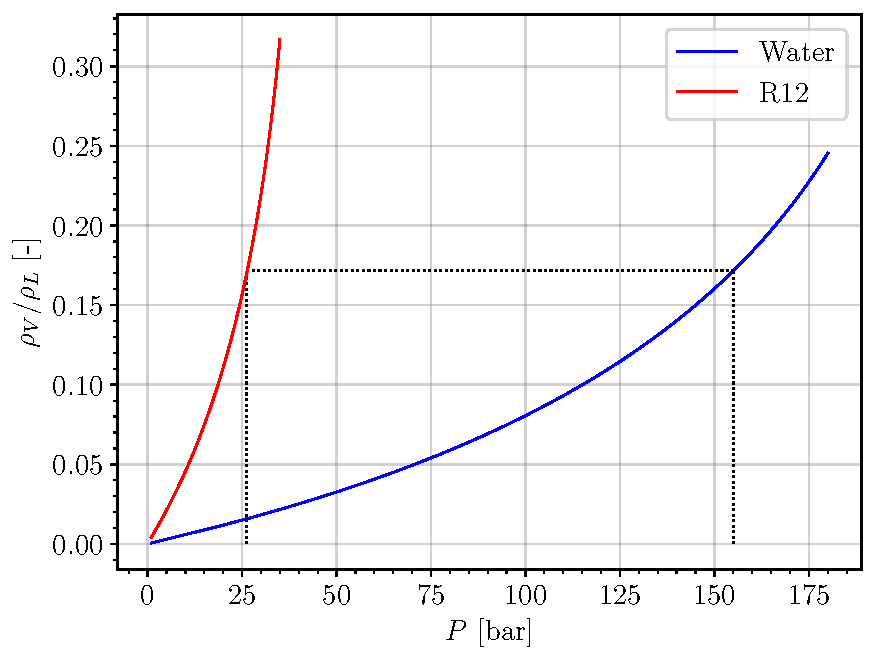
\includegraphics[width=0.6\linewidth]{img/DEBORA/rhost_R12_PWR.pdf}
\caption{Density ratio of pressurized R12 and water}
\label{fig:rhost_R12_PWR}
\end{figure}


For instance, we can see that R12 at approximatively 26 bar ($T_{sat} \approx 86.8 \degC$) has the same density ratio as water at 155 bar ($T_{sat} \approx 344.8 \degC$).

\npar

\begin{note*}{}
This tranposition criteria thus scales the operating pressure $P$ of the experiment.
\end{note*}

\subsection{Conservation of the Weber Number}

The Weber number is also similar to those encountered in PWR.

\begin{equation}
\We = \dfrac{G^{2}R}{\rho_{L} \sigma}
\end{equation}

This number characterizes physical phenomena such as bubble break-up or deformation under the influence of the liquid inertia.

\begin{figure}[!h]
\centering
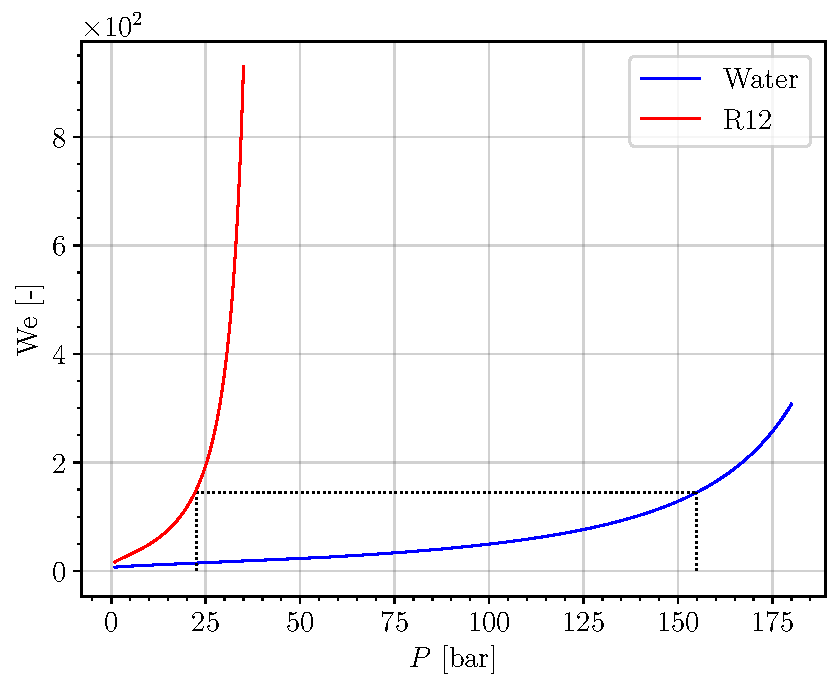
\includegraphics[width=0.6\linewidth]{img/DEBORA/We_R12_PWR.pdf}
\caption{Weber number for R12 and water at $G=2000~\debm$ and $R=0.1\mm$}
\label{fig:We_R12_PWR}
\end{figure}

Similar to the phase density ratio, Figure \ref{fig:We_R12_PWR} shows that Weber number equivalent to water at 155 bar can be reached with  R12 around 23 bar.

\npar

\begin{note*}{}
For a same value of $R$, this transposition scales the inlet liquid mass flux $G$.
\end{note*}

\subsection{Conservation of the Boiling Number}

The boiling number is defined as :

\begin{equation}
\Bo = \frac{\phi_{w}}{G h_{LV}}
\end{equation}  

It represents the comparison between the vapor mass flux $\phi_{w}/h_{LV}$ if all the heat flux contributes to phase change versus the inlet liquid mass flux. Thus, its value can be associated to the boiling and two-phase flow regime.

\begin{figure}[!h]
\centering
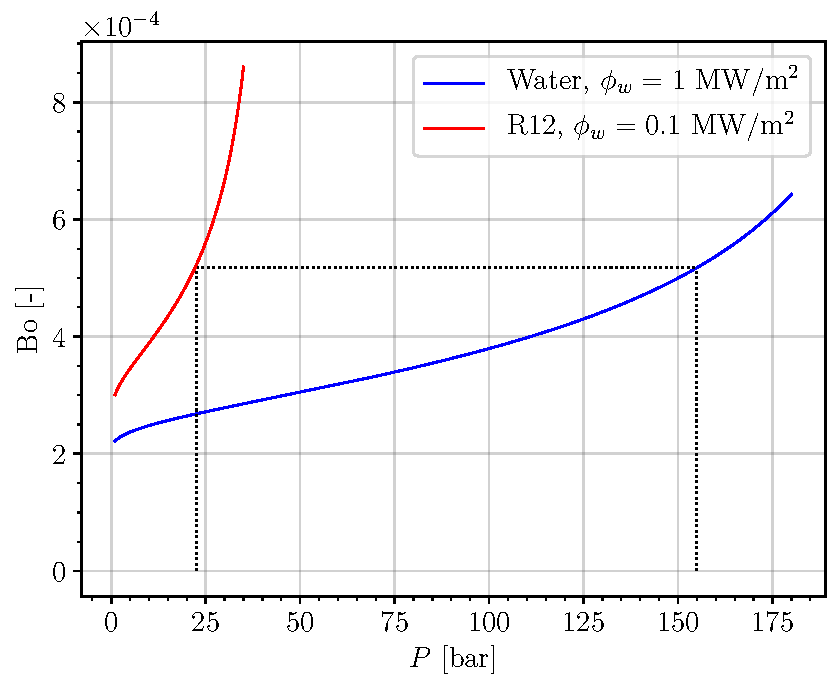
\includegraphics[width=0.6\linewidth]{img/DEBORA/Bo_R12_PWR.pdf}
\caption{Boiling number for R12 and water at $G = 2000~\debm$}
\label{fig:Bo_R12_PWR}
\end{figure}

Figure \ref{fig:Bo_R12_PWR} shows that Boiling number values similar to PWR can be reproduced using R12 with wall heat fluxes one order of magnitude lower and pressure around 23 bar.


\begin{note*}{}
This transposition criteria scales the applied heat flux $\phi_{w}$.
\end{note*}

\subsection{Conservation of the Inlet Thermodynamic Quality}

Water in PWR being highly subcooled to avoid boiling, reproducing the inlet subcooling in the DEBORA experiment allows to mimic the early stages of boiling between the ONB and OSV. It allows to reproduce Boiling Crisis by Departure from Nucleate Boiling for low quality flows. This is achieved through the inlet thermodynamic quality:


\begin{equation}
x_{eq,in} = \frac{h_{L,in} - h_{L,sat}}{h_{LV}}
\end{equation}

\begin{note*}{}
This transposition is achieved by scaling the R12 inlet temperature.
\end{note*}

\subsection{Same Geometry}

The last similarity achieved in the DEBORA experiment is related to the geometry. The heated length $L_{ch}$ of the test section is similar to the height of a nuclear fuel assembly and the hydraulic diameter $D_{h}$ is equal to that of a subchannel.


\subsection{Transposition ranges}

As a result of those conservation criteria, Table \ref{tab:R12_PWR_transposition} sums up the transposition ranges for each parameters.



\begin{table}[!h]
\centering
\begin{tabular}{c||c|c} 

Fluid & Water & Freon R12 \\
\hline \hline
$P$ [bar] & 100 - 180 & 14 - 30\\
%
$G$ [$\debm$] & 1000 - 5000 & 1000 - 5000\\
%
$\phi_{w}$ [MW/m$^{2}$] & 0.5 - 6 & 0.05 - 0.65\\ 
%
$x_{eq,in}$ [-] & (-0.4) - (+0.4) & (-0.4) - (+0.4)\\
\hline
\hline 
${\rho_{V,sat}}/{\rho_{L,sat}}$ [-] & 0.08 - 0.25 & 0.07 - 0.22\\
%
$\We$ [-] & 49.5 - 307.1 & 69.1 - 365.8\\
%
$\Bo \times 10^{-3} $ [-] &  $0.19$ - $3.86$ & $0.21$ - $4.33$ \\
\hline
\end{tabular}

\caption{Water R12 scaling, $R=0.01$mm for $\We$}
\label{tab:R12_PWR_transposition}

\end{table}



\section{Description of the Test Section}

\subsection{Geometrical Description}
To apply the aforementioned transport criteria, four thermal-hydraulic control parameters are imposed in the test section :

\begin{itemize}
\item The outlet pressure $P$ ;
\item The inlet mass flow rate $G \times S_{in}$ with $S_{in} = \pi R^{2} \approx 2.9 \times 10^{-4}$ m\up{2} the inlet area ;
\item The inlet liquid temperature $T_{L,in}$ ;
\item The electrical power transferred to the liquid $\phi_{w}\times S_{heat}$ with $S_{heat}$ the heated area. 
\end{itemize}

\begin{figure}[!h]
\centering
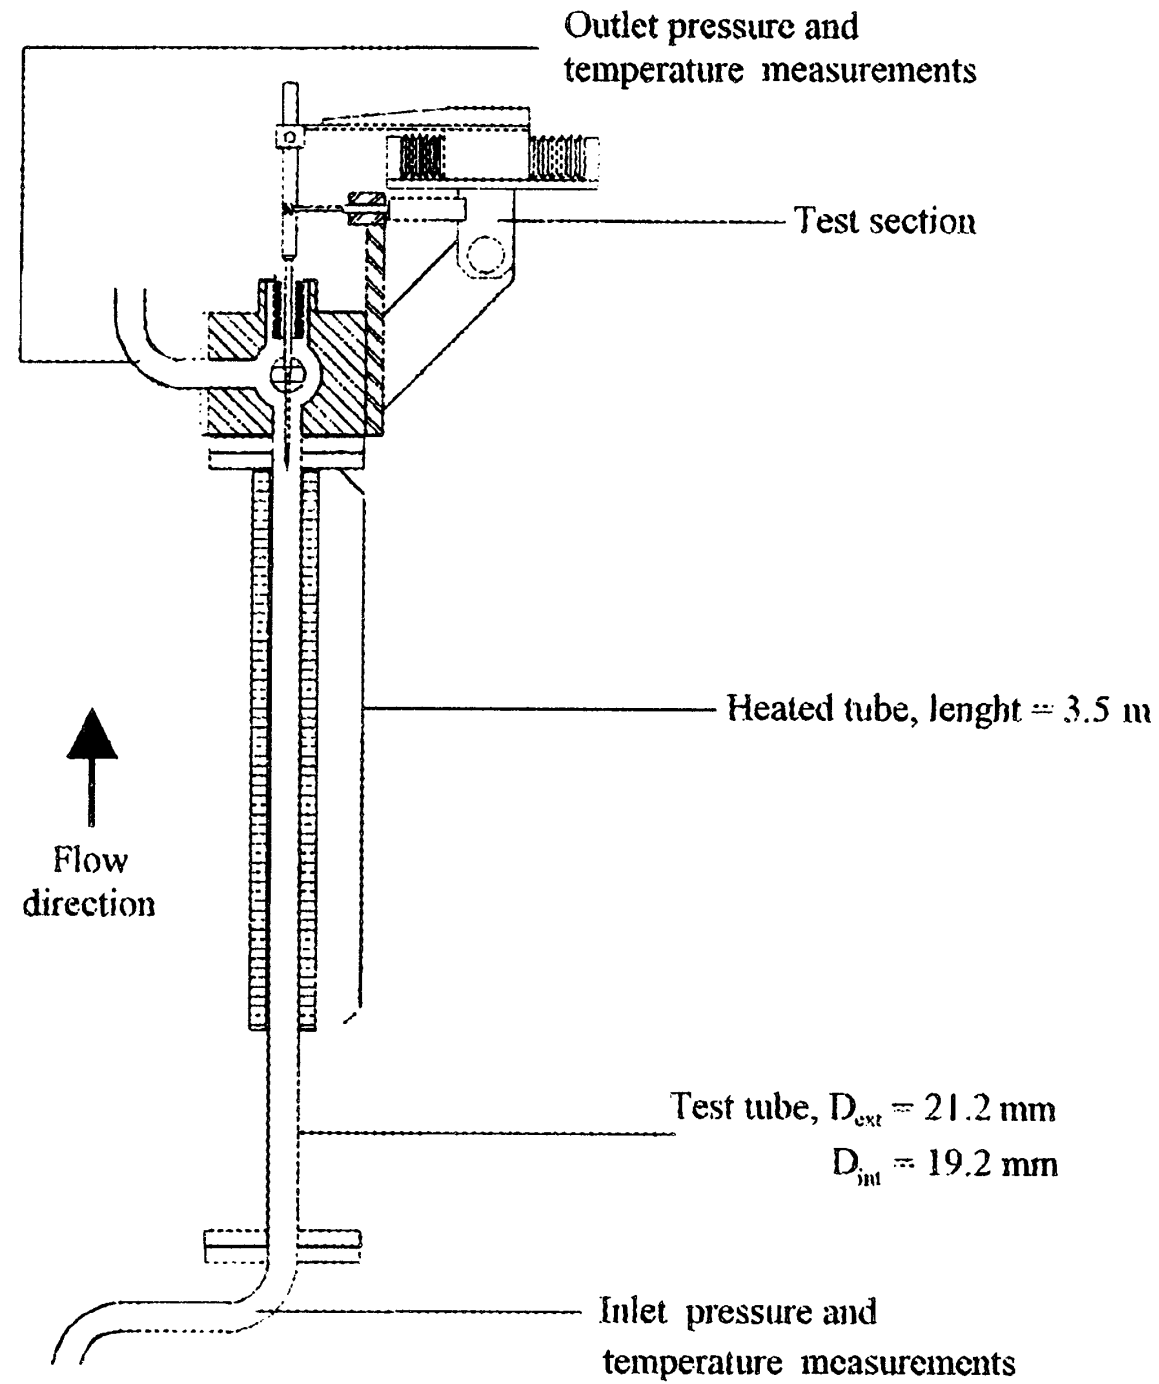
\includegraphics[width=0.5\linewidth]{img/DEBORA/debora_sketch.png}
\caption{Sketch of the DEBORA test section. Adapted from \cite{garnier_local_2001}.}
\label{fig:sketch_debora}
\end{figure}


The test section in presented on Figure \ref{fig:sketch_debora}. It consists of an inconel tube with inner diameter $D_{h}=19.2$ mm, a 1 mm thickness and a heated length $L_{heat}$=3.5 m. A detailed description of the whole experimental loop is given in Garnier \etal \cite{garnier_local_2001}.

\subsection{Measurement Instrumentation}

The control parameters are adjusted and measured using pressure, temperature, flow rate and power measurements. They are further detailed in Cubizolles \cite{Cubizolles_1996}.

\npar

The local measurements are conducted at the end of the heating length using a controllable probe that can cover the whole diameter of the test section with an accuracy of $10 \mu$m . Only one diameter is covered since the chosen geometry induces an axisymmetry.

Three type of measurements have been conducted over different experimental campaigns.

\subsubsection{Mono-Optical Probe Measurements}


Optical probe measurement rely on the difference of optical refractive index between the liquid and vapor phase. Using an optical fiber in which light is emitted towards the probe tip allows to detect the actual phase flowing on the probe. 

\npar

The resulting signal is called a Phase Indicator Function (PIF) which looks like to a square signal (Figure \ref{fig:FIP}) that can be post-processed to identify the average time spent by the probe in each phase and then estimate their volume fraction \eg the void fraction. 


\begin{figure}[!h]
\centering
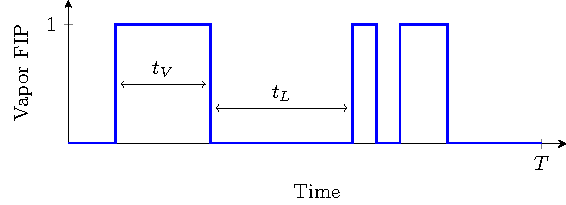
\includegraphics[width=0.65\linewidth]{img/DEBORA/FIP.pdf}
\caption{Example of Phase Indicator Function signal}
\label{fig:FIP}
\end{figure}



If the PIF is measured over a period $T$, the void fraction $\alpha$ at the measurement point $x$ can be estimated by :


\begin{equation}
\alpha\parth{x}\ = \nu\parth{x} \overline{t_{V}} = \frac{1}{T} \sum t_{V}
\end{equation}
where $\nu$ is called the interference frequency that represents the number of phase interface detection per second by the probe.

\begin{remark*}{}
This measurement technique was performed in the \textbf{measurement campaign C2900} where void fraction profiles at the outlet were obtained for various flow conditions.
\end{remark*}

\subsubsection{Bi-Optical Probe Measurements}


Using the technology of the optical phase dectection, adding a second optical probe permits to measure more parameters of the two-phase flow. Indeed, the use of two probes placed close to each other with a small shift in the flow direction (Figure \ref{fig:optical_probe}) allows to estimate the velocity of the interface between the two probes by measuring the time difference between the two PIF.


\begin{figure}[!h]
\centering
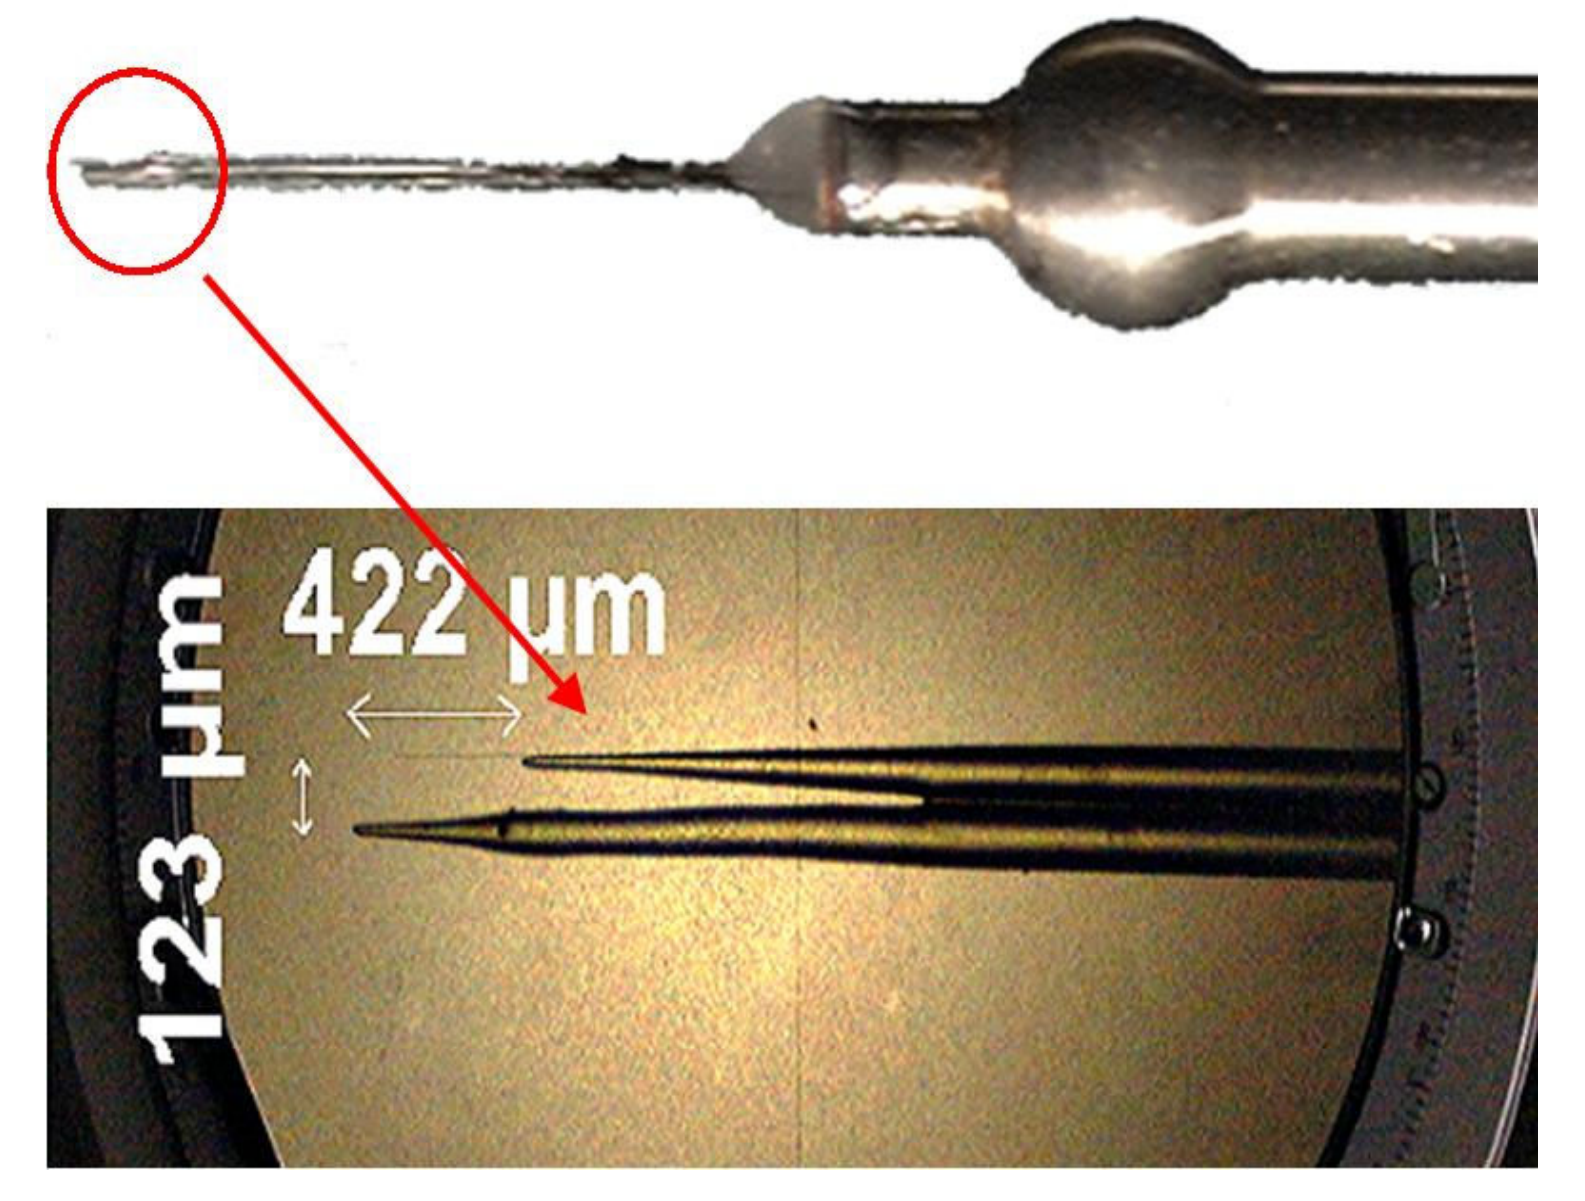
\includegraphics[width=0.65\linewidth]{img/DEBORA/optical_probe.png}
\caption{Picture of the bi-optical probe with a zoom over the two optical fibers. Reproduced from \cite{gueguen_phd}.}
\label{fig:optical_probe}
\end{figure}

\npar

Considering the following assumptions :

\begin{itemize}
\item The flow is mainly one-directional in aligned with the probes ;
\item The vapor phase is composed of spherical inclusions ;
\item The velocity gradient and center density gradient are small along a bubble diameter length.
\end{itemize}

Then we can estimate : 

\begin{itemize}
\item The vapor axial velocity $U_{V,z}$ that can be supposed equal to the measured interface velocity between the probes ;
\item The interfacial area density $a_{i}$ :
\begin{equation}
a_{i} = \frac{4 \nu }{U_{V,z}}
\end{equation}
\item The bubble Sauter diameter :
\begin{equation}
D_{V} = \frac{6 \alpha }{a_{i}}
\end{equation}
\end{itemize}


\begin{remark*}{}
This measurement technique was performed in the \textbf{measurement campaign C3000}.
\end{remark*}


\subsubsection{Thermocouples Measurements}

Thermal measurements are conducted using chromel-alumel thermocouples. The liquid temperature is measured along the outlet diameter at the end of the heating length. Wall temperature measurements are conducted with 4 thermocouples placed at different heights (1.465 m, 2.465 m, 2.965 m, 3.485 m) on the outside of the tube.

\begin{remark*}{}
This measurement technique was performed in the \textbf{measurement campaign C800}.
\end{remark*}



\section{Measurements Campaigns and Results}

\subsection{Cases Nomenclature and Test Series}

As mentioned before, three different campaigns have been performed :

\begin{itemize}
\item Campaign C2900 with solely void fraction measurements using mono-optical probe ;

\item Campaign C3000 with void fraction, vapor velocity, bubble Sauter diameter and interfacial area density measurements using bi-optical probe ;

\item Campaign C800 with liquid and wall temperature measurements using thermocouples.
\end{itemize}


Each measurement series is conducted under fixed outlet pressure, liquid mass flux and electrical power. Inlet temperature is then changed to cover different inlet quality. Experimental cases are named in the form C\textbf{cc}G\textbf{g}P\textbf{pp}W\textbf{ww}Te\textbf{tt} with \textbf{cc} the campaign number (29, 30 or 8), \textbf{g} the inlet mass velocity ($G$ in t/m\up{2}/s), \textbf{pp} the outlet pressure ($P$ in bars), \textbf{ww} the total heat power applied ($\Phi_{w}$ in kW) and \textbf{tt} the inlet temperature ($T_{L,in}$ in K). For instance, the case named C30G2P26W16Te66 has been conducted with $P=26.2$ bar, $G=2049\ \debm$, $\Phi_{w}=15.6$ kW $\equiv$ $\phi_{w} =73.89$ kW/m\up{2} and $T_{L,in} = 66.59 \degC$.


\begin{table}[!h]
\scriptsize
\centering


\noindent\makebox[\textwidth]{
\renewcommand{\arraystretch}{2.0}
\begin{tabular}{|c|c|c|c|c|c|c|c|c|c|c|c|c|c|c|c|c|c|c|}
\hline
P                   & G & W16 & W17 & W23 & W24 & W25 & W27 & W29 & W30 & W31 & W33 & W34 & W36 & W38 & W39 & W40 & W42 & W44 \\
\hline
\hline
\multirow{3}{*}{14} & 2 &  $\bigcirc$ $\bigtriangledown$ $\bigtriangleup$  & $\bigtriangleup$    &     &  $\bigcirc$   &     &     &     &     &     &     &     &     &     &     &     &     &     \\
                    & 4  &     &     &     &  $\bigcirc$   &     &     &     &     &     &     &     &     &     &     &     &     &     \\
                    & 5  &     &     &     &     &     &     & $\bigtriangledown$    &  $\bigtriangledown$   &     &  $\bigtriangledown$   &  $\bigtriangledown$   &  $\bigtriangledown$   &   $\bigtriangledown$  &    & $\bigtriangledown$   &  $\bigtriangledown$   &     \\
                    \hline
\multirow{3}{*}{26} & 2  &  $\bigcirc$ $\bigtriangledown$ $\bigtriangleup$  &     &     &     &     &     &     &     &     &     &     &     &     &     &     &     &     \\
                    & 3 &     &     &  $\bigtriangledown$ $\bigtriangleup$  &     &  $\bigtriangledown$   &  $\bigtriangledown$ $\bigtriangleup$   &   $\bigtriangledown$  &     & $\bigtriangledown$  $\bigtriangleup$   &  $\bigtriangledown$   &     &  $\bigtriangledown$   $\bigtriangleup$ &  $\bigtriangledown$   &  $\bigtriangledown$   & $\bigtriangledown$ $\bigtriangleup$   & $\bigtriangledown$    &  $\bigtriangledown$ $\bigtriangleup$   \\
                    & 5  & $\bigcirc$   &     &     &  $\bigcirc$   &     &     &     &     &     &     &     &     &     &     &     &     &     \\
\hline
\end{tabular}
}

\npar

\noindent\makebox[\textwidth]{
\renewcommand{\arraystretch}{2.0}
\begin{tabular}{|c|c|c|c|}
\hline
P                   & G & W12 & W14\\
\hline
\hline
30                  & 1 &  $\bigtriangledown$   &  $\bigtriangledown$   \\
\hline
\end{tabular}
}

\caption{Test matrix of the DEBORA cases. $\bigcirc$ : C800 - $\bigtriangledown$ : C2900 - $\bigtriangleup$ : C3000 }%\newline \scriptsize{Written at Plateau d'Auguste, Hyper U, Saintes} }
\label{tab:debora_matrix}
\end{table}


If we want to obtain a full description of the two-phase flow from the DEBORA tests, we need to have measurements from campaigns C3000 and C800 (flow topology and thermal) with the same control parameters. Table \ref{tab:debora_matrix} unfortunately shows that only very few test series between C3000 and C800 have common operating conditions, namely :

\begin{itemize}
\item Series 8G2P14W16 and 30G2P14W16 ;
\item Series 8G2P26W16 and 30G2P26W16.
\end{itemize}

Other flow conditions have either been covered with thermal measurements or topology measurements but not both. 

\begin{remark*}{}
Cases from the campaign C2900 would only be relevant for void fraction profiles comparison. Estimations of the bubble diameter can not be achieved except if one assumes a velocity profile as suggested by Cubizolles \cite{cubizolles_phd} and re-used by Guéguen \cite{gueguen_phd} who supposes :

\begin{equation}
U_{V,z} \approx U_{M,z} = 1.22 G \parth{ \frac{R-r}{R}}^{1/7}
\label{eq:ugz_C29}
\end{equation}
where $U_{M,z}$ is the mixture axial velocity, assuming a mechanical equilibrium between the phases.

\end{remark*}


For further studies, we will mainly focus on the G2P26W16 and G2P14W16 test series. Although we will mainly rely on the results from the C3000 campaign (where vapor velocity was actually measured) for flow topology qualification, we will evaluate the assumption of Eq. \ref{eq:ugz_C29} with the C2900 measurements.


\subsection{Verification of Control Parameters Coherency}

For each case, the total heat heat input $\Phi_{w}$ is given along with the inlet mass flux $G$, inlet liquid temperature $T_{L,in}$ and outlet quality $x_{eq,out}$. To verify the consistency of those values, we can recalculate the outlet quality :

\begin{equation}
x_{eq,out,calc} = \frac{h_{M,out,calc} - h_{L,sat}}{h_{LV}}
\label{eq:xeq_out}
\end{equation}
with $h_{M,out,calc}$ the recalculated outlet mixture enthalpy  :

\begin{equation}
h_{M,out,calc} = h_{in} + \frac{\Phi_{w}}{G S_{in}} = h_{in} + \frac{4\phi_{w}L_{heat}}{G D_{h}}
\end{equation}
with $h_{in}$ the inlet enthalpy calculated from the fluid properties using the inlet liquid temperature.

\npar
The difference between the given and recalculated outlet quality can also be converted to input power error by recalculating the heat needed to reach the given $x_{eq,out}$  :

\begin{equation}
\Phi_{w,calc} = \frac{G  \pi R^{2}}{\underbrace{\crocht{x_{eq,out}h_{LV}+h_{L,sat}}}_{h_{M,out}} - h_{L,in}}
\end{equation}

\npar 


Moreover, for a given set of experiments at the same $P$, $G$ and $\Phi_{w}$ changing the inlet quality can be associated to moving the measurement diameter along the axial direction following the relationship : 

\begin{equation}
x_{eq}\parth{z} = x_{eq,in} + \frac{4 \phi_{w} z }{G D_{h} h_{LV}}
\end{equation}

Thus, taking the maximum inlet quality case $x_{eq,in, max}$ as a reference ($z=3.5$ m), we can estimate the corresponding measurement height $z_{eq}$ of each other cases if the inlet quality was $x_{eq,in, max}$.

\npar

We calculated the equivalent heights and outlet quality / power input errors for two series of the C3000 campaigns. Results are displayed on Tables \ref{tab:30P14_recalc} and \ref{tab:30P26_recalc}.



\begin{table}[!h]
\centering
\begin{tabular}{c|c|c|c|c|c|c}
$T_{L,in}$ {[}K{]} & $x_{eq,in,calc}$ {[}-{]} & $x_{eq,out,calc}$ {[}-{]} & $x_{eq,out}$ {[}-{]} & $z_{eq}$ {[}m{]} & $x_{eq,out}$ error {[}-{]} & $\Phi_{w}$ error {[}kW{]} \\
\hline
\hline
22.39  &  -0.317  &  -0.0821  &  -0.0832  &  1.075  &  0.114 \% &  -0.078 \\
%
26.8  &  -0.28  &  -0.0422  &  -0.0431  &  1.653  &  0.089 \% &  -0.061\\
%
28.76  &  -0.263  &  -0.0267  &  -0.0273  &  1.896  &  0.056 \% &  -0.038\\
%
30.08  &  -0.252  &  -0.0152  &  -0.0157  &  2.065  &  0.05 \% &  -0.034\\
%
31.39  &  -0.241  &  -0.004  &  -0.0043  &  2.234  &  0.035 \% &  -0.023\\
%
38.95  &  -0.175  &  0.0674  &  0.0681  &  3.229  &  -0.072 \% &  0.049\\
%
39.96  &  -0.166  &  0.077  &  0.0776  &  3.357  &  -0.063 \% &  0.042\\
%
41.16  &  -0.155  &  0.0875  &  0.0882  &  3.509  &  -0.064 \% &  0.043
\end{tabular}
\caption{Recalculated control parameters for the 30G2P14W16 cases. ($T_{sat} = 58.07\degC$)}
\label{tab:30P14_recalc}
\end{table}


\begin{table}[!h]
\centering
\begin{tabular}{c|c|c|c|c|c|c}
$T_{L,in}$ {[}K{]} & $x_{eq,in,calc}$ {[}-{]} & $x_{eq,out,calc}$ {[}-{]} & $x_{eq,out}$ {[}-{]} & $z_{eq}$ {[}m{]} & $x_{eq,out}$ error {[}-{]} & $\Phi_{w}$ error {[}kW{]} \\
\hline
\hline
58.57              & -0.395                   & -0.0893                   & -0.0819              & 1.792            & -0.747 \%                  & 0.381                     \\
60.54              & -0.370                   & -0.0650                   & -0.0578              & 2.072            & -0.722 \%                  & 0.369                     \\
62.54              & -0.344                   & -0.0392                   & -0.0318              & 2.369            & -0.741 \%                  & 0.378                     \\
64.6               & -0.318                   & -0.0123                   & -0.0050              & 2.674            & -0.736 \%                  & 0.376                     \\
66.59              & -0.292                   & 0.0140                    & 0.0213               & 2.973            & -0.728 \%                  & 0.371                     \\
68.57              & -0.266                   & 0.0402                    & 0.0473               & 3.271            & -0.716 \%                  & 0.365                     \\
70.59              & -0.239                   & 0.0670                    & 0.0743               & 3.583            & -0.723 \%                  & 0.369                    
\end{tabular}
\caption{Recalculated control parameters for the 30G2P26W16 cases. ($T_{sat} = 86.81\degC$)}
\label{tab:30P26_recalc}
\end{table}

As we can see, the given values of outlet quality for the 30G2P14W16 tests are coherent with the one-dimensional enthalpy balance with errors mostly less than 0.1\% on the recalculated quality and less than 100 W on the recalculated power input. This naturally leads to an equivalent height very close to $3.5$ m for the hottest case.


However, a more significant error is observed on the 30G2P26W16 cases where errors up to 0.75\% on the outlet quality and close to 0.4 kW on the power input are found. Those values are significant especially for cases close to saturation where uncondensed vapor will start to appear in the bulk. Moreover, this results in an equivalent height 8.3 cm longer than the actually 3.5m heated length.

\npar

Since the inlet temperature, mass flux and power input are controlled parameters for each test, it is likely that the error may come from the given value of outlet quality $x_{eq,out}$ which is calculated and not imposed.

\begin{note*}{}
Similar quality / input power errors were obtained on corresponding C29 and C8 campaigns :

\begin{itemize}
\item Negligible errors on for 29G2P14W16 and 8G2P14W16 cases ;
\item Roughly 0.7 \% outlet quality error and 0.3 to 0.4 kW power error for 29G2P26W16 and 8G2P26W16 cases. 
\end{itemize}
\end{note*}

\subsection{Qualitative Analysis of the Experimental Results}

On Figures \ref{fig:30G2P26W16_exp}, \ref{fig:8G2P26W16_exp}, \ref{fig:30G2P14W16_exp} and \ref{fig:8G2P14W16_exp} we respectively plot the experimental measurements of cases 29/30G2P26W16, 8G2P26W16, 29/30G2P14W16 and 8G2P14W16. The colorbar representing the oulet quality of each test is based on the computed value of $x_{eq,out}$ (Eq. \ref{eq:xeq_out}).


\subsubsection{G2P26W16 cases}

\begin{figure}[h!]
\centering

\subfloat[Void fraction measurements]{
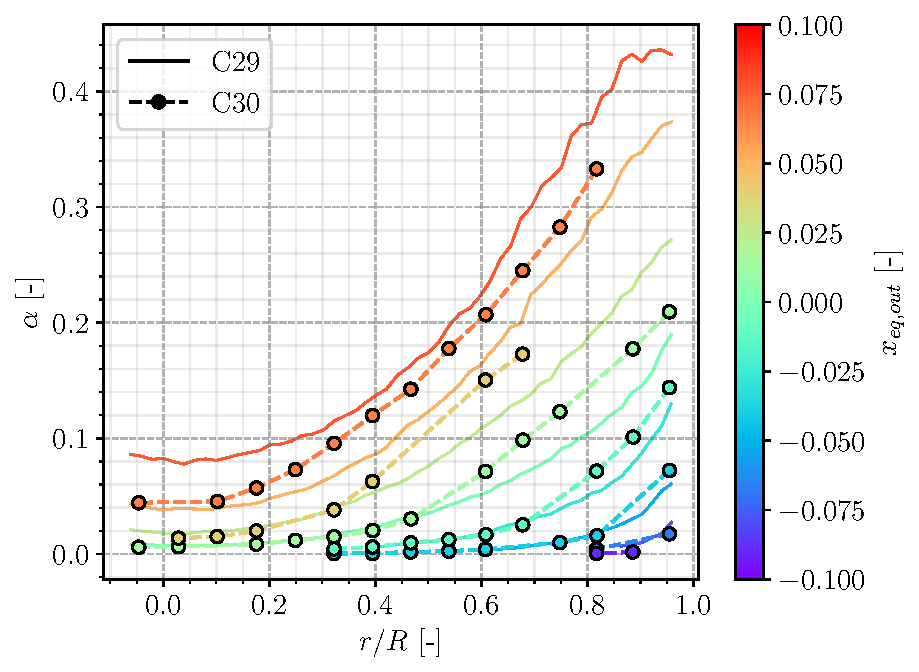
\includegraphics[width=0.5\linewidth]{img/DEBORA/30G2P26W16/30G2P26W16_alpha.pdf}
\label{fig:G2P26W16_alpha}
}
\subfloat[Vapor velocity measurements]{
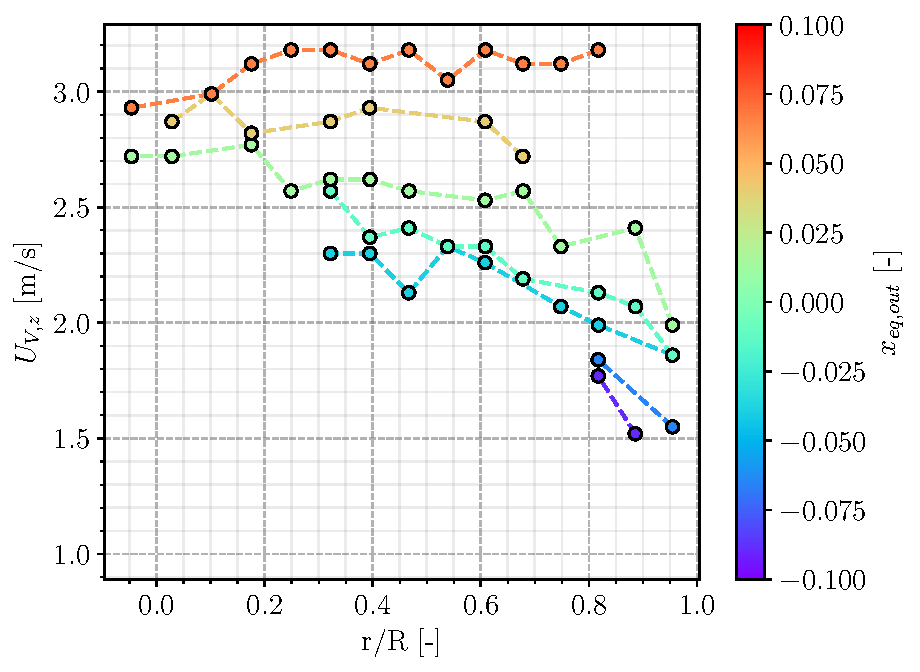
\includegraphics[width=0.5\linewidth]{img/DEBORA/30G2P26W16/30G2P26W16_ugz.pdf}
\label{fig:G2P26W16_ugz}
}
\\
\subfloat[Bubble diameter measurements]{
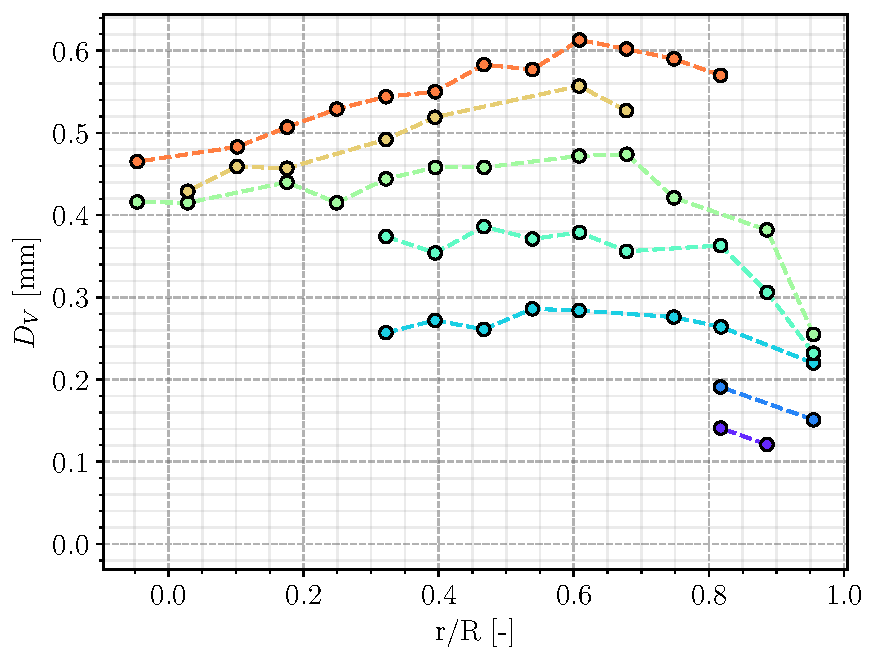
\includegraphics[width=0.5\linewidth]{img/DEBORA/30G2P26W16/30G2P26W16_dv.pdf}
\label{fig:G2P26W16_dv}
}
\subfloat[Interfacial area concentration measurements]{
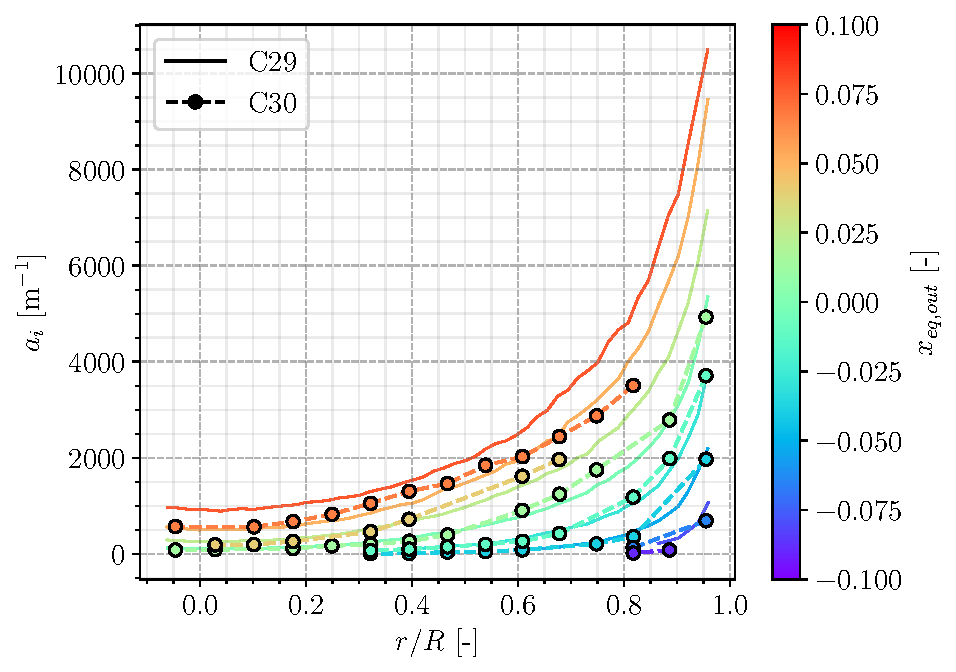
\includegraphics[width=0.5\linewidth]{img/DEBORA/30G2P26W16/30G2P26W16_ai.pdf}
\label{fig:G2P26W16_ai}
}


\caption{30G2P26W16 and 29G2P26W16 results}
\label{fig:30G2P26W16_exp}
\end{figure}

Void fraction profiles obtained in for C2900 (single optical probe) and C3000 (bi-optical probe) cases are compared to verify the consistency of the measurements (Figure \ref{fig:G2P26W16_alpha}). The two campaigns are in good agreement with each other, displaying a void fraction profile monotonously increasing with the outlet quality. The estimation of the vapor velocity by Eq. \ref{eq:ugz_C29} for the C29 results is acceptable but presents an growing underestimation as the outlet title increases (Figure \ref{fig:G2P26W16_ugz}). This results in bubble diameter underestimation close to the wall and consequently interfacial area overestimation. 

\npar

We observe that the void fraction naturally increases with the outlet quality and that we reach net vapor generation with $\alpha\parth{R=0} > 0$ when $x_{eq,out}>0$. Otherwise, vapor is not detected over the whole measurement section. Each case has its maximum void fraction near the wall with values up to approximately $40\%$ when the outlet quality approaches 0.1.

\npar

The bubble diameter displays different behaviors (Figure \ref{fig:G2P26W16_dv}) : 

\begin{itemize}
\item It grows from the wall and reaches a maximum around $r/R \approx 0.6$, indicating bubble coalescence ;
\item It stays nearly constant for negative outlet quality cases ;
\item It decreases from $r/R = 0.6$ to $r/R = 0$ for saturated cases , indicating either bubble break-up or bulk condensation.
\end{itemize}

\begin{remark*}{}
It seems that bubble diameter very close to the wall do not vary much between different cases, indicating that bubbles leave the wall at a nearly constant diameter over the different explored liquid temperatures ($D_{V} \approx 0.2$ mm).
\end{remark*}

\npar

Vapor velocity also increases with the outlet quality, with a nearly flat profile reached for saturated cases. The increase in vapor velocity may result of the larger bubble diameters which enhance the effect of buoyancy, acting as an accelerating term increasing the drift velocity.

\begin{remark*}{}
Eq. \ref{eq:ugz_C29} fails to predict this flattening of the vapor velocity on C2900 cases, which may indicate a change in the flow structure that can not be detected when assuming liquid-vapor mechanical equilibrium.
\end{remark*}

\npar

\begin{figure}[h!]
\centering

\subfloat[Liquid subcooling profiles]{
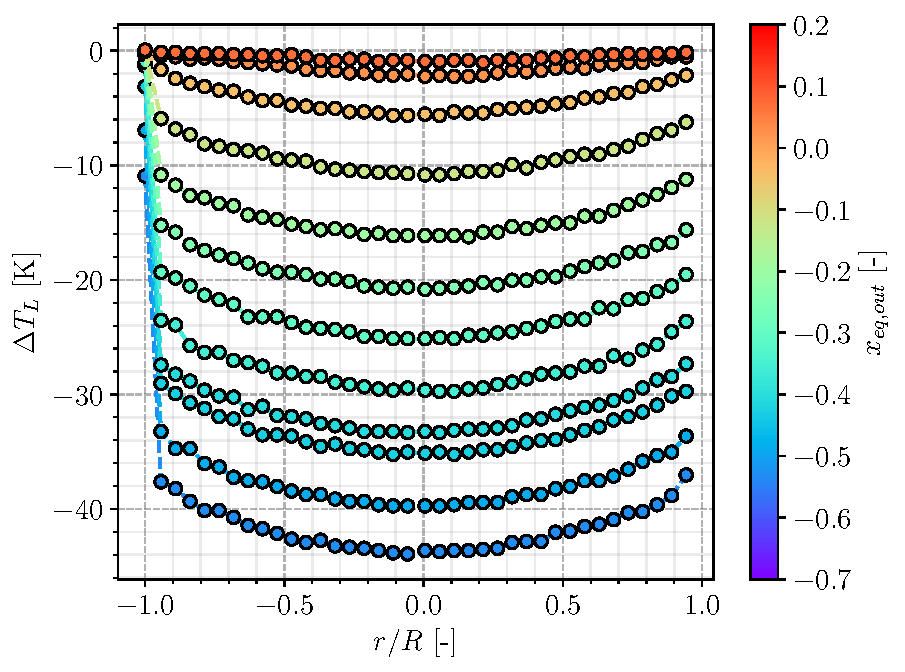
\includegraphics[width=0.5\linewidth]{img/DEBORA/8G2P26W16/8G2P26W16_TL.pdf}
\label{fig:G2P26W16_TL}
}
\subfloat[Liquid subcooling profiles (zoom)]{
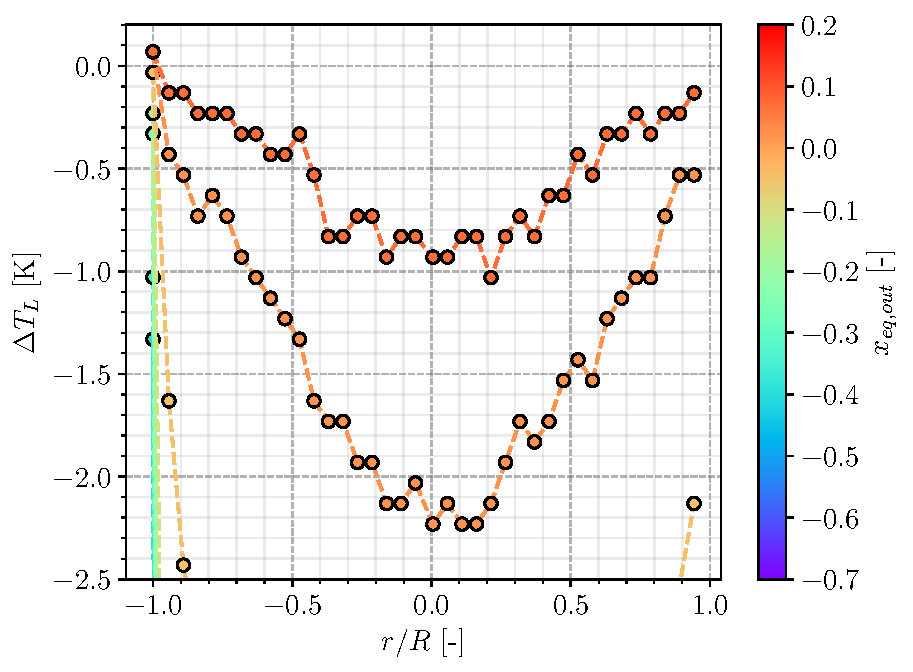
\includegraphics[width=0.5\linewidth]{img/DEBORA/8G2P26W16/8G2P26W16_TLSH.pdf}
\label{fig:G2P26W16_TL_zoom}
}
\\
\subfloat[Wall superheat vs. axial position]{
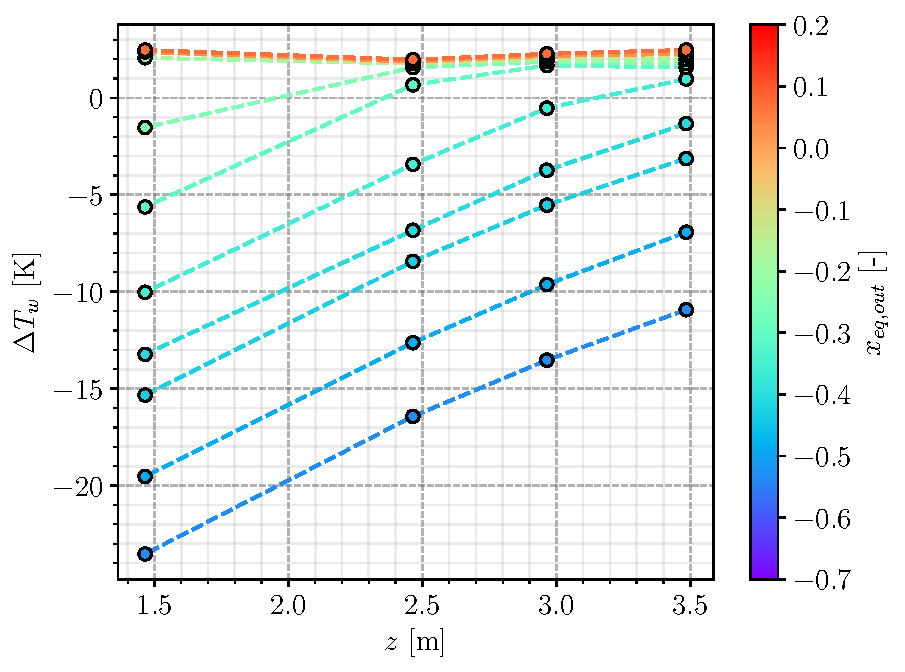
\includegraphics[width=0.5\linewidth]{img/DEBORA/8G2P26W16/8G2P26W16_Tw_z.pdf}
\label{fig:G2P26W16_Twz}
}
\subfloat[Wall superheat vs. local flow quality]{
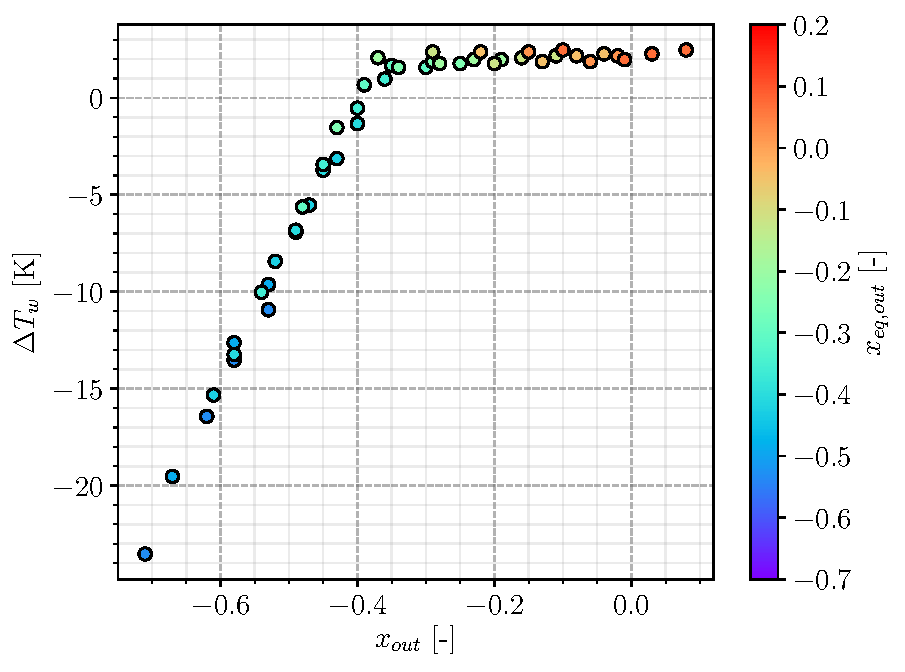
\includegraphics[width=0.5\linewidth]{img/DEBORA/8G2P26W16/8G2P26W16_Tw_x.pdf}
\label{fig:G2P26W16_Twx}
}


\caption{8G2P26W16 results}
\label{fig:8G2P26W16_exp}
\end{figure}

Regarding the liquid temperature measurements (Figures \ref{fig:G2P26W16_TL} and \ref{fig:G2P26W16_TL_zoom}), we see that temperature profiles linearly rise with the inlet quality while presenting an unmodified parabolic shape. The only change appears when reaching significant superheated conditions ($x_{eq,out} \sim 0.1$) where the liquid temperature profile flattens over the test section. 

Moreover, we observe that measurements very close to the wall present a very large temperature gradient even for low quality cases (temperature jump of nearly 30 degrees for coldest cases). This jump reduces as flow quality increases and reduces even more for boiling cases, indicating the well-known rise of the global heat transfer coefficient in boiling regime vs. single-phase convection regime.

We can also note that for the hottest case, the liquid becomes superheated near the wall ($\Delta T_{L}\parth{\pm 1} \approx 0.1\degC$). The bulk is still slightly subcooled with $\Delta T_{L}\parth{0} = -1\degC$

\begin{remark*}{}
The liquid being subcooled in the bulk for superheated cases hints that the decrease in bubble diameter observed in Figure \ref{fig:G2P26W16_dv} for $r/R < 0.6$ may be associated to condensation.
\end{remark*}

\npar

Wall temperature measurements (Figures \ref{fig:G2P26W16_Twz}) display linear growth for subcooled cases which is in agreement with traditional liquid convection problems. When reaching boiling, the wall superheat stabilizes at $\Delta T_{w} \approx 2\degC$.
Rearranging the different wall temperature measurements versus the local flow quality (Figure \ref{fig:G2P26W16_Twx}) presents a coherent overlapping between cases with different inlet subcooling. This further validates the transposition of inlet quality into variation into an evolution of the measurement probe's axial position.


\subsubsection{G2P14W16 cases}


\begin{figure}[h!]
\centering

\subfloat[Void fraction measurements]{
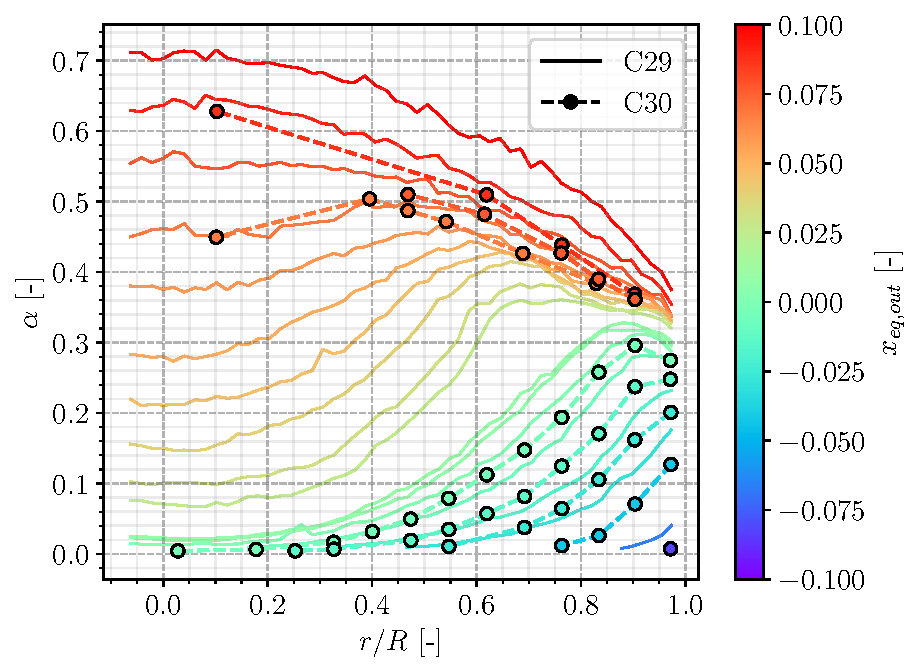
\includegraphics[width=0.5\linewidth]{img/DEBORA/30G2P14W16/30G2P14W16_alpha.pdf}
\label{fig:G2P14W16_alpha}
}
\subfloat[Vapor velocity measurements]{
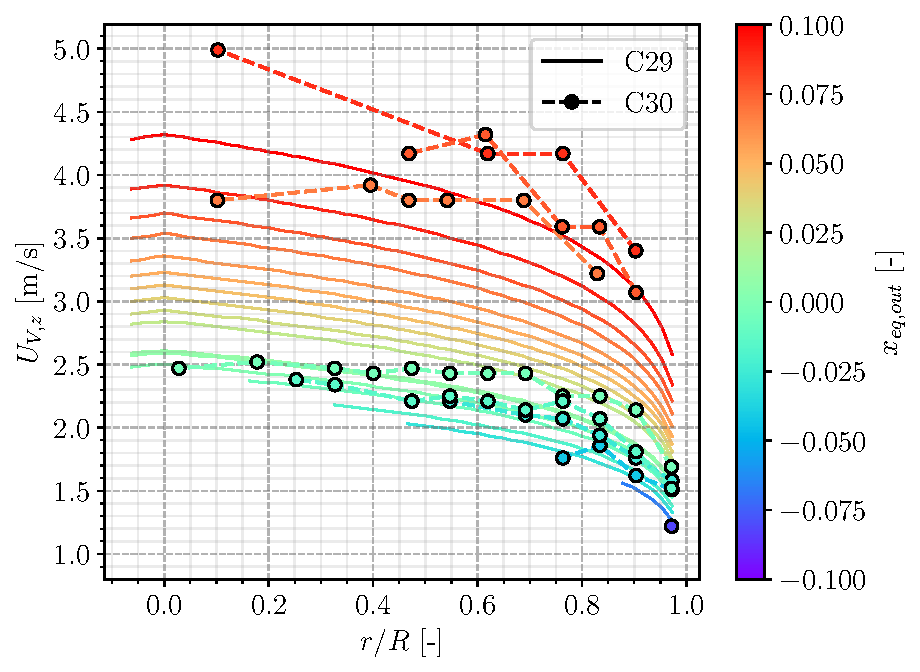
\includegraphics[width=0.5\linewidth]{img/DEBORA/30G2P14W16/30G2P14W16_ugz.pdf}
\label{fig:G2P14W16_ugz}
}
\\
\subfloat[Bubble diameter measurements]{
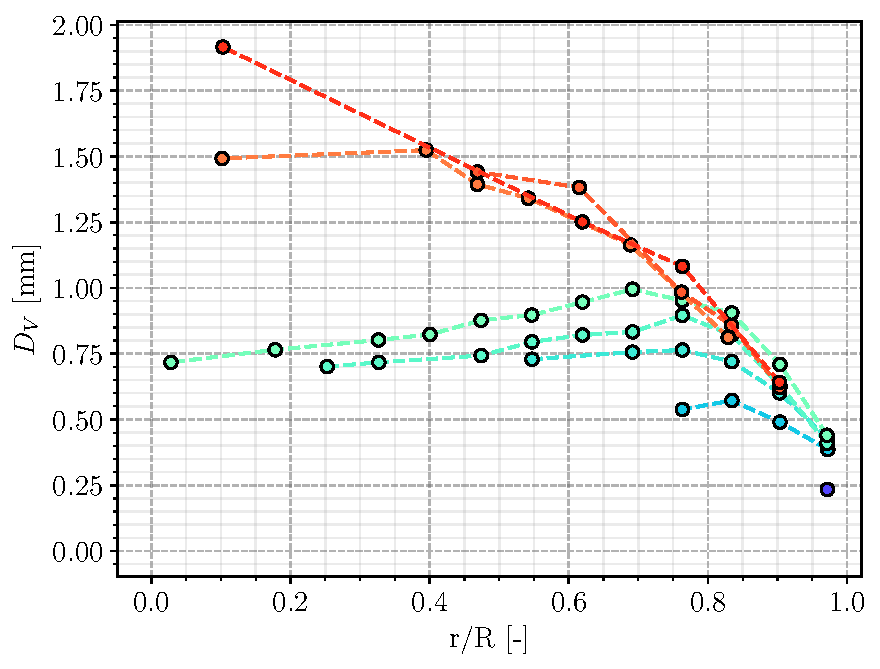
\includegraphics[width=0.5\linewidth]{img/DEBORA/30G2P14W16/30G2P14W16_dv.pdf}
\label{fig:G2P14W16_dv}
}
\subfloat[Interfacial area concentration measurements]{
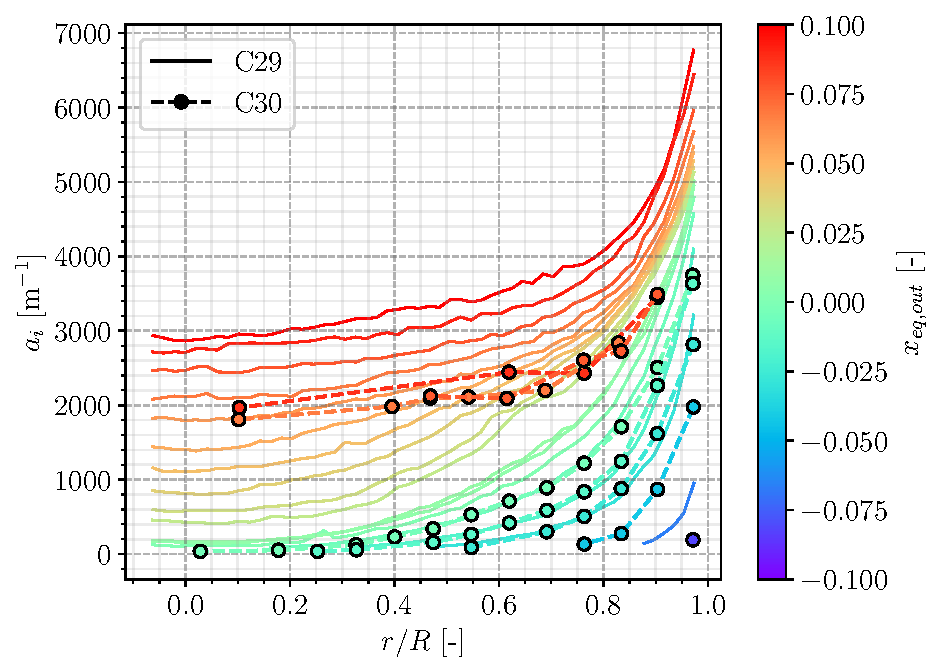
\includegraphics[width=0.5\linewidth]{img/DEBORA/30G2P14W16/30G2P14W16_ai.pdf}
\label{fig:G2P14W16_ai}
}

\caption{30G2P14W16 and 29G2P14W16 results}
\label{fig:30G2P14W16_exp}
\end{figure}



Similar to the G2P26W16 cases, we observe the consistency of the void fraction measurements between the C2900 and C300 campaigns (Figure \ref{fig:G2P14W16_alpha}). Although the vapor velocity estimation using Eq. \ref{eq:ugz_C29} for C2900 cases also produces acceptable results for subcooled cases, the discrepancy when saturation is reached is even more observed here (Figure \ref{fig:G2P14W16_ugz}). The overestimation when $x_{eq,out}>0$ is larger than for the G2P26W16 cases, with nearly 1 m/s error on hottest cases. 

This logically yields larger underestimations of the bubble diameter and associated overestimations of the interfacial area concentration.

\npar

The void fraction profiles (Figure \ref{fig:G2P14W16_alpha}) present a particular evolution with a moving $\alpha$ peak that shifts from the wall to the bulk as the outlet quality increases. This may indicate a particular bubble dynamics regime inducing transverse bubble migration and accumulation far from the wall. Bulk void fraction can reach values as high as 70\% with a flattening profile when $x_{eq,out} \to 0.1$.

\begin{remark*}{}
It seems that saturated cases tend to reach a fixed value of near-wall void fraction between 35\% and 40\%.
\end{remark*}

\npar

Similar to previous obervations, the bubble diameter grows when moving to the bulk, also presenting a peak value around $0.8 > r/R > 0.6$ for subcooled cases (Figure \ref{fig:G2P14W16_dv}). The saturated cases however present much larger increase in bubble diameter when reaching the bulk flow, with $D_{V}$ close to 2 mm for the hottest case. This definitely indicates predominant coalescence effects.

\begin{remark*}{}
$D_{V}\approx 2$ mm is observed at a point where $\alpha >60\%$ which shows that even at such high void fraction values, the flow is still in a bubbly regime with small vapor inclusions ($D_{V} \approx 0.1 D_{h}$).
\end{remark*}

\npar

The vapor velocity also increases with the outlet quality (Figure \ref{fig:G2P14W16_ugz}), but reaches much larger value compared to the G2P26W16 cases. This may be due to the larger bubble size and local void fractions associated to the imposed mass flow rate.


\begin{figure}[h!]
\centering

\subfloat[Liquid subcooling profiles]{
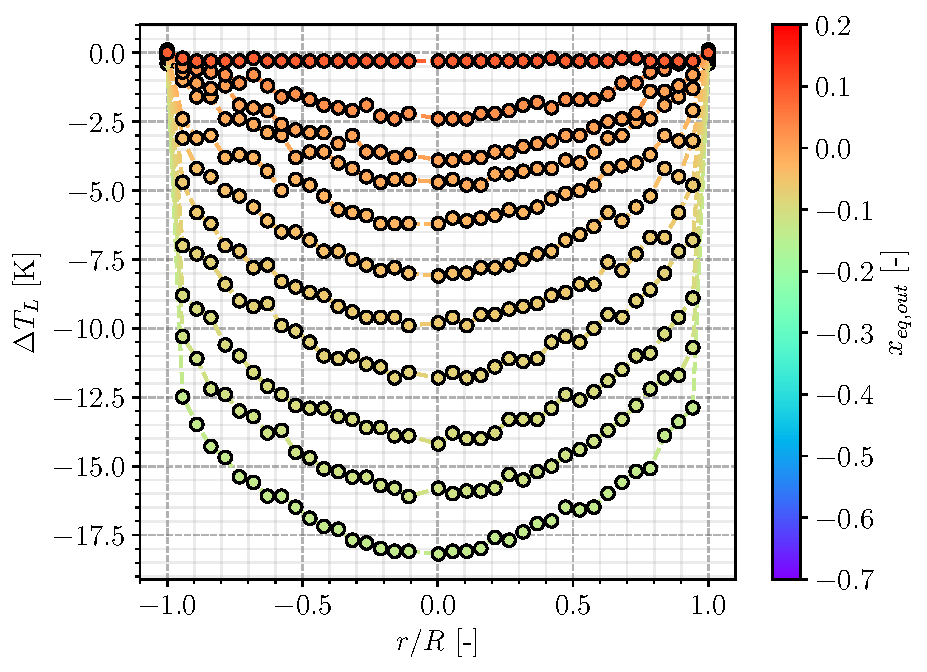
\includegraphics[width=0.5\linewidth]{img/DEBORA/8G2P14W16/8G2P14W16_TL.pdf}
\label{fig:G2P14W16_TL}
}
\subfloat[Liquid subcooling profiles (zoom)]{
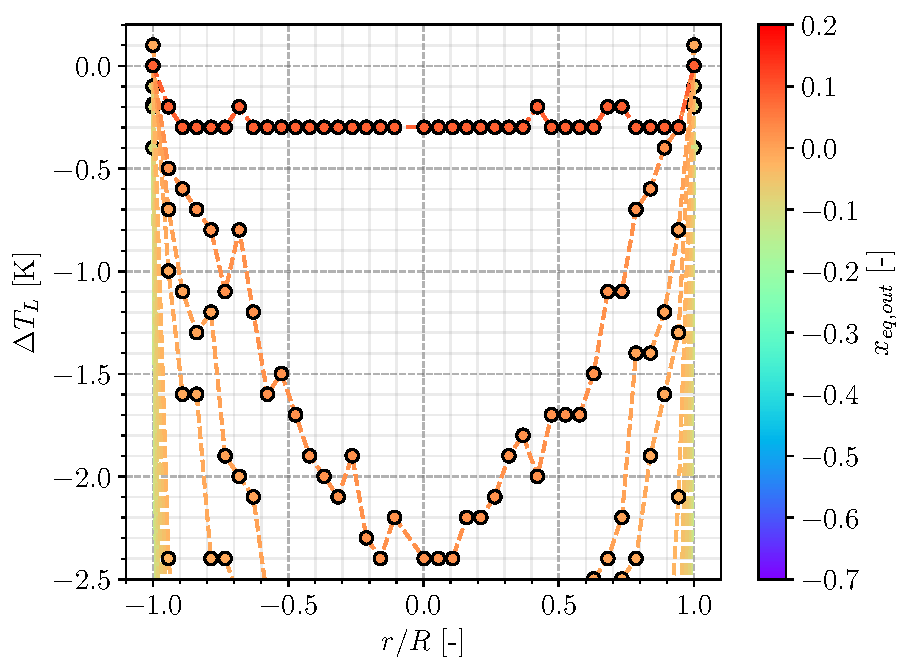
\includegraphics[width=0.5\linewidth]{img/DEBORA/8G2P14W16/8G2P14W16_TLSH.pdf}
\label{fig:G2P14W16_TL_zoom}
}
\\
\subfloat[Wall superheat vs. axial position]{
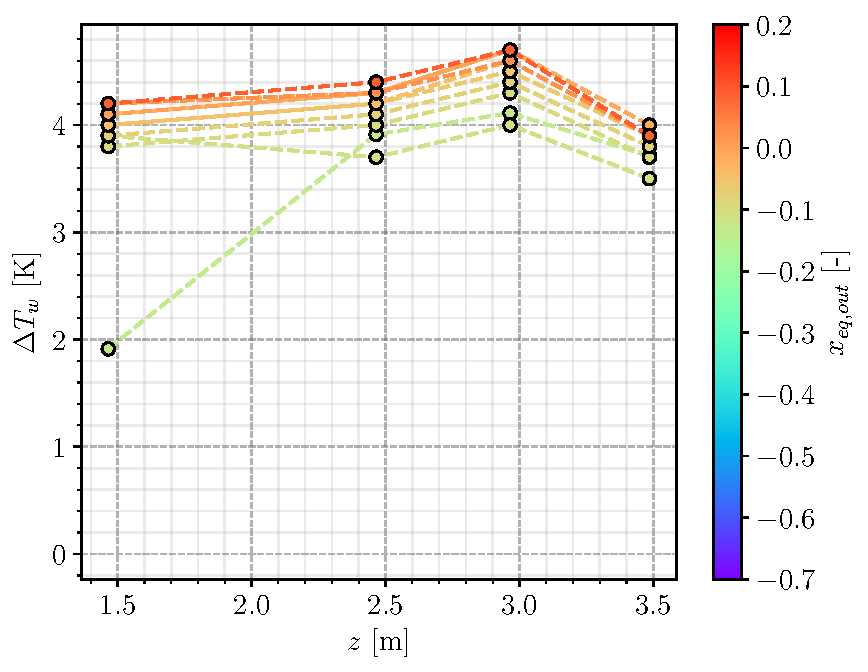
\includegraphics[width=0.5\linewidth]{img/DEBORA/8G2P14W16/8G2P14W16_Tw_z.pdf}
\label{fig:G2P14W16_Twz}
}
\subfloat[Wall superheat vs. local flow quality]{
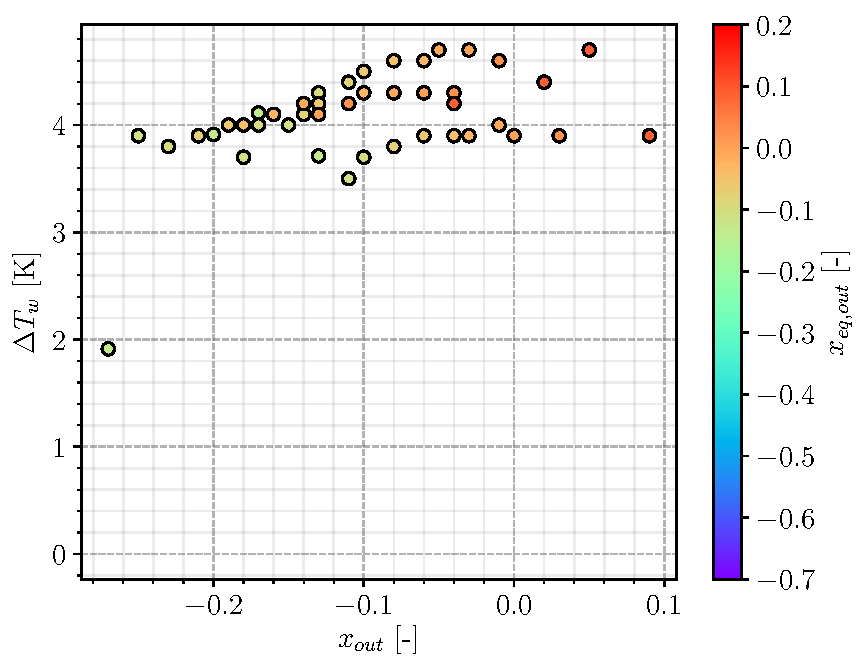
\includegraphics[width=0.5\linewidth]{img/DEBORA/8G2P14W16/8G2P14W16_Tw_x.pdf}
\label{fig:G2P14W16_Twx}
}


\caption{8G2P14W16 results}
\label{fig:8G2P14W16_exp}
\end{figure}


\npar

The liquid temperature profiles (Figure \ref{fig:G2P14W16_TL}) are behaving in a very similar way to the G2P26W16 cases (Figure \ref{fig:G2P26W16_TL}) : stable parabolic profile, linear shift with inlet quality and flattening when reaching superheated conditions ($x_{eq,out} \sim 0.1$).

We also have the huge temperature jump when approaching the wall which reduces when reaching boiling regimes. The measurements also detect superheated liquid near the wall for the hottest cases ($\Delta T_{L} \approx 0.1 \degree$). The case with the greatest outlet quality presents a surprisingly flat liquid temperature profile with measurements being nearly constant ($\Delta T_{L}=-0.3\degC$) over the whole measurement section. 

\begin{remark*}{}
Such a constant temperature profile could be interpreted as a limit of the liquid temperature in this regime. Since it corresponds to flow conditions where void fraction is large ($\alpha > 60\%$) and bubbles do not condense (Figure \ref{fig:G2P14W16_dv}), any extra heat input may only contribute to phase change and leave the liquid phase thermally unchanged.
\end{remark*}

\npar

Unfortunately, the 8G2P15W16 campaign did not cover as large quality range as the 8G2P26W16 campaign. We thus do not have access to many single-phase flow wall temperature measurements (Figure \ref{fig:G2P14W16_Twz}). Only one point for $x_{eq,out} \approx -0.1$ seem to be in the single-phase convection region. All the other measurements are close to each other and correspond to boiling regimes where we observe a wall superheat stabilization aroud $\Delta T_{w} = 4\degC$.

The comparison of wall temperature with local flow quality (Figure \ref{fig:G2P14W16_Twx}) is not as interesting as the G2P26W16 cases but still display a welcomed overlapping of the measurements over the different inlet temperatures.


\section{Further Verifications}


\subsection{Reconstruction of the Applied Heat Flux}

To further quantify the coherency of the DEBORA database, we want to reconstruct the wall heat flux injected in the flow from the experimental measurements of void fraction, vapor velocity and liquid temperature measurements.

\subsubsection{Methodology}

To do so, we will estimate the total enthalpy change between the inlet and outlet. The inlet liquid enthalpy $h_{L,in}$ is estimated using the inlet temperature and the outlet mixture enthalpy $h_{M,out}$ is computed as :

\begin{equation}
h_{M,out}=x_{eq,out}h_{V,sat}+\parth{1-x_{eq,out}}\spavg{h_{L,out}}
\end{equation}
supposing that the vapor is at saturation temperature.

\npar
Using the experimental values of $\alpha$ and $U_{V,z}$, we can recompute the outlet quality $x_{eq,out}$ as :

\begin{equation}
x_{eq,out} = \frac{\rho_{V}\spavg{\alpha U_{V,z}}}{G}
\end{equation}

where :

\begin{equation}
\spavg{\alpha U_{V,z}} = \frac{1}{\pi R^{2}}\int_{\vartheta=0}^{2\pi} \int_{r=0}^{R} \alpha\parth{r} U_{V,z}\parth{r} r \mathrm{d}r \mathrm{d}\vartheta = \frac{2}{R^{2}}\int_{r=0}^{R}  \alpha\parth{r} U_{V,z}\parth{r} r \mathrm{d}r
\end{equation}
for an axisymmetric profile such as the DEBORA measurements.

Similarly, the average liquid enthaly at the outlet is estimated from the average liquid temperature $\spavg{T_{L}}$ and the R12 equation of state.

\npar

Then, writing the one-dimensional energy balance of the flow permits to express the actually applied heat flux : 

\begin{equation}
G \pi R^{2} \parth{h_{M,out} - h_{L,in}} = \Phi_{w} = \phi_{w} 2\pi R L_{heat} \ \Rightarrow \phi_{w} = \frac{\parth{h_{M,out}-h_{L,in}}GR}{2L_{heat}}
\end{equation}
which can be compared to the given control parameter for the experiment.

\subsubsection{Application}

To apply the presented reconstruction of the heat flux, we either need : 

\begin{itemize}
\item A pure single-phase case with an outlet liquid temeprature profile (C800 case alone);
\item A boiling two-phase case with void fraction and vapor velocity measurements (C3000 case) along with liquid temperature (C800 case).
\end{itemize}

This means that for boiling cases, we need to "merge" cases from the C3000 and C800 campaign conducted in very close operating conditions ($P$, $G$, $T_{L,in}$) and assume that the liquid temperature measurements of the C800 case are actually representative of the liquid temperature in the C3000 case and reciprocally for the void fraction and vapor velocity.

\npar

Such a constraint leaves us with very few boiling cases that can accommodate this conditions. They are summed up on Table \ref{tab:debora_match_C8C30}.


\begin{table}[!h]
\centering

\begin{tabular}{c||c|c|c|c|c|c}
Case Name & $P$ [bar] & $G$ [kg/m$^{2}$/s]  & $\phi_{w}$ [kW/m$^{2}$]& $T_{L,in}$ [$\degC$] & $x_{eq,in}$ [-] & $x_{eq,out}$ [-] \\
\hline
\hline
30G2P26W16Te66  &  26.2  &  2049.0  &  73.893  &  66.59  &  -0.2919  &  0.014 \\
8G2P26W16Te66.6  &  26.2  &  1982.0  &  73.9  &  66.57  &  -0.2927  &  0.0237 \\
\hline 
30G2P26W16Te70  &  26.19  &  2051.2  &  73.893  &  70.59  &  -0.2386  &  0.067 \\
8G2P26W16Te70.3  &  26.2  &  1983.0  &  73.9  &  70.31  &  -0.2428  &  0.0734 \\
\hline
\hline
30G2P14W16Te40  &  14.59  &  2007.8  &  77.688  &  41.16  &  -0.1555  &  0.0875 \\
8G2P14W16Te43.1  &  14.6  &  2014.0  &  72.9  &  43.08  &  -0.1387  &  0.0889 \\
\end{tabular}

\caption{Similar conditions cases between the C3000 and C800 campaigns. Outlet quality calculated with Eq. \ref{eq:xeq_out}.}
\label{tab:debora_match_C8C30}
\end{table}




\begin{table}[!h]
\centering

\begin{tabular}{c||c|c|c|c|c}
\hline
Cas & $x_{eq,out}$ [-] & $\spavg{T_{L}}$ [$\degC$] & $\phi_{w,rec}$ [kW/m$^{2}$] & $\phi_{w,exp}$ [kW/m$^{2}$] & $\Delta \phi_{w}$ [\%]  \\
\hline
\hline
30G2P26W23Te66.6 & 1.931\% & 85.71 & 70.914 & 73.893 & -4.03\%\\
\hline
30G2P26W23Te70.6 & 4.998\% & 86.73 & 69.482 & 73.893 & -5.97\%\\
\hline
\hline
30G2P14W16Te40 & 0 & 0 & 0 & 0 & 0
\end{tabular}

\caption{Heat flux recalculation results}
\label{tab:debora_flux_corr_res}

\end{table}


\subsection{Comparison with One Dimensional Correlations}

\subsection{Experimental Heat Flux Corrections}

\chapter{NEPTUNE\_CFD simulations of DEBORA cases}

In this work, we present the simulations of the following cases :
\begin{itemize}
\item C8G2P26W16Te44.9 and C8G2P26W16Te49.6 (single-phase flow)
\item C8G2P26W16Te66.6 and C8G2P26W16Te70.3 (two-phase flow)
\item C30G2P26W16Te66.6 and C30G2P26W16Te70.6 (two-phase flow)
\end{itemize}

The pressure of $26~\text{bar}$ is chosen to match the pressure of the mixing vanes cases (DEBORA-Promoteur, Section \ref{sec:deb_prom}). Mesh sensitivity is performed over two meshes : a large mesh (M1) with $460~356\text{ cells }=338\text{ radial } \times 1362 \text{ axial cells}$ and a fine mesh (M2) with $3~157~952\text{ cells }=1568\text{ radial } \times 2014 \text{ axial cells}$.

On Figure \ref{fig:th_1phi_res}, we present the results regarding liquid temperature at the outlet and wall temperature. The liquid temperature profile seems to be correctly reproduced by the simulations, though we see a slight overestimation close to the wall. Looking closer at boiling cases shows a difference of $\approx 0.5\degree$ C, which is close to the uncertainty of the measurements \cite{Garnier2001}. Concerning the wall temperature, it appears that it is underestimated before the \textbf{Onset of Nucleate Boiling} (ONB) ($T_{w}<T_{sat}$) and overestimated after the ONB ($\approx +5\degree$C). Post-ONB wall temperature is characterized by a stabilization of its value above the saturation temperature (here $T_{w,ONB}-T_{sat}\approx 2\degree\text{C}$).

%
\begin{figure}[h!]
\centering
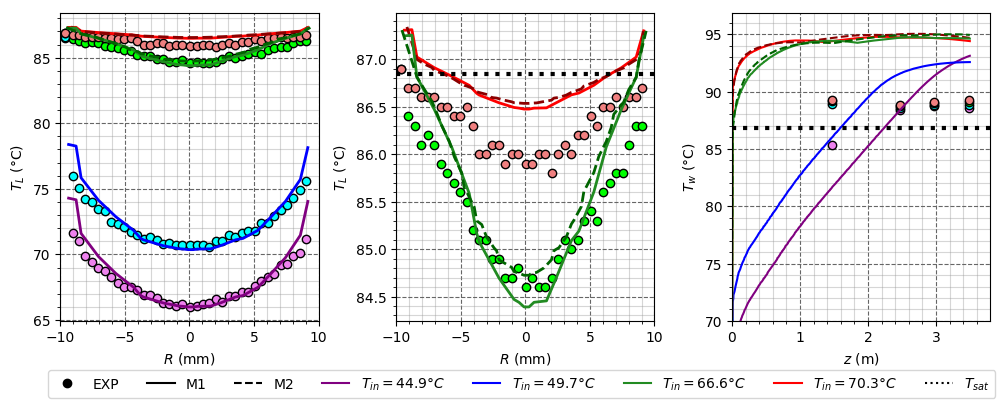
\includegraphics[scale=0.60]{img/DEBORA/c8.png}
\caption{NCFD (lines) vs. Exp. (circles) - $T_{L}$ and $T_{w}$ - Cases C8G2P26W16Te44.9, Te49.6, Te66.6 and Te70.3 - Simulations using two meshes M1 (coarse) and M2 (fine).}
\label{fig:th_1phi_res}
\end{figure}
%

%%
%\begin{figure}[!htb]
%\vspace{16pt}
%\begin{spacing}{1.0}
%\centering
%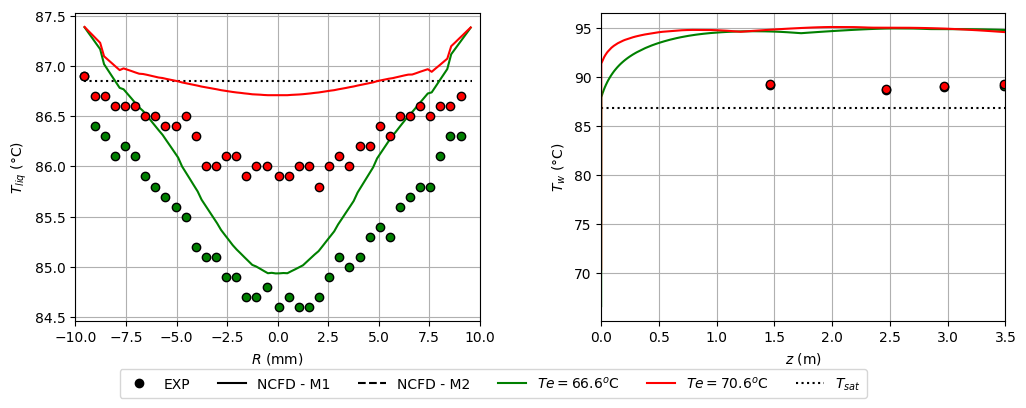
\includegraphics[scale=0.60]{img/DEBORA/thermal_diph.png}
%\caption{NEPTUNE\_CFD simulations results vs. experimental measurements - $T_{L}$ and $T_{w}$ - Cases C8G2P26W16Te66.6 and C8G2P26W16Te70.3}
%\label{fig:th_diph_res}
%\end{spacing}
%\vspace{16pt}
%\end{figure}
%%



%
\begin{figure}[h!]
\centering
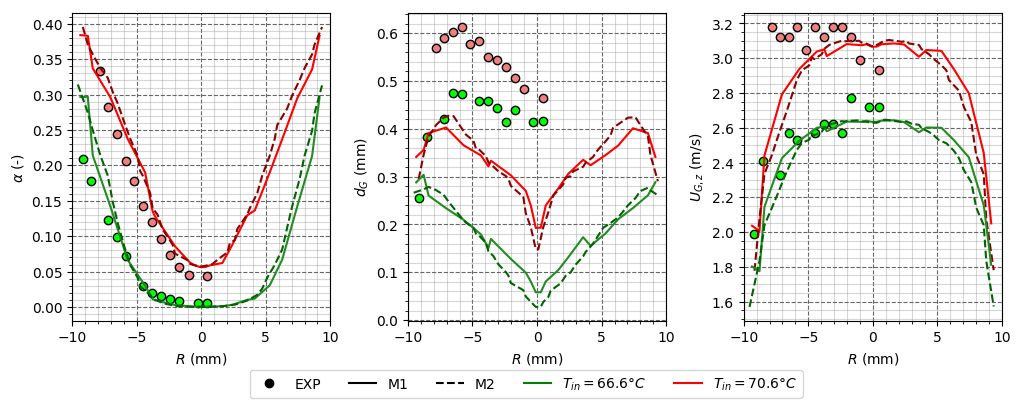
\includegraphics[scale=0.60]{img/DEBORA/c30.png}
\caption{NCFD (lines) vs. Exp. (circles) - $\alpha$, $d_{G}$ and $U_{G,z}$ - Cases C30G2P26W16Te66.6 and Te70.6 - Simulations using two meshes M1 (coarse) and M2 (fine).}
\label{fig:topology_res}
\end{figure}
%

On Figure \ref{fig:topology_res}, we compare the results of the simulations to the experiments regarding void fraction, bubble Sauter diameter and axial gas velocity. Void fraction profiles are quite correctly reproduced, though we observe a $10\%$ higher peak at the wall for $T_{in}=66.6\degree$C. The order of magnitude of bubble diameter is correct ($\sim 0.1\text{mm}$) and NEPTUNE\_CFD manages to detect coalescence (increase of bubble diameter when leaving the wall) and bulk condensation (decrease of bubble diameter when reaching the core of the flow), which is in qualitative agreement with the experiments. Quantitatively speaking, bubble diameter is globally underestimated. Finally, gas velocity profile is reasonably reproduced for $T_{in}=66.6\degree$C, but not for $T_{in}=70.6\degree$C. The latter experimental profile is flatter, which could be explained by a change of flow regime since uncondensed vapor is detected in the bulk.  

Finally, the simulations reasonably agree with the experiments. The strongest discrepancies being mostly the wall temperature and bubble diameter. Potential ways of improving those results are investigated in next sub-section.

\subsection{Investigating the nucleation site density modeling $N_{sit}$}

In NEPTUNE\_CFD, wall temperature is computed through the Heat Flux Partitioning model, which role is to find the appropriate $T_{w}$ which balances Equation $\ref{eq:HFP}$. However, some laws used to express parameters such as $N_{sit}$, $f$, or $d_{d}$ are quite old and simple. For instance, the {Lemmert} \& {Chawla}\cite{Lemmert1977} expression of $N_{sit}$ only depends on the wall superheat (Sub-section \ref{subsec:HFP}).%, meaning that it can not reproduce potential influence of the pressure on the nucleation site density.

A comparison of the {Lemmert} \& {Chawla} law\cite{Lemmert1977} with  the {Hibiki} \& {Ishii}\cite{Hibiki2003} law for $N_{sit}$ against 4 data sets from the literature is presentend on Figure \ref{fig:nsit}. The {Hibiki} \& {Ishii} correlation depends simultaneously on wall superheat, pressure and contact angle.  Experimental measurements of {Borishanskii} \etal\cite{Borishanskii1961}, {Richenderfer} \etal\cite{Richenderfer2018}, {Kossolapov} \etal\cite{Kossolapov2020} and {Zhou} \etal\cite{Zhou2020} are used to assess the two nucleation site density correlations.
%
\begin{figure}[h!]
\centering
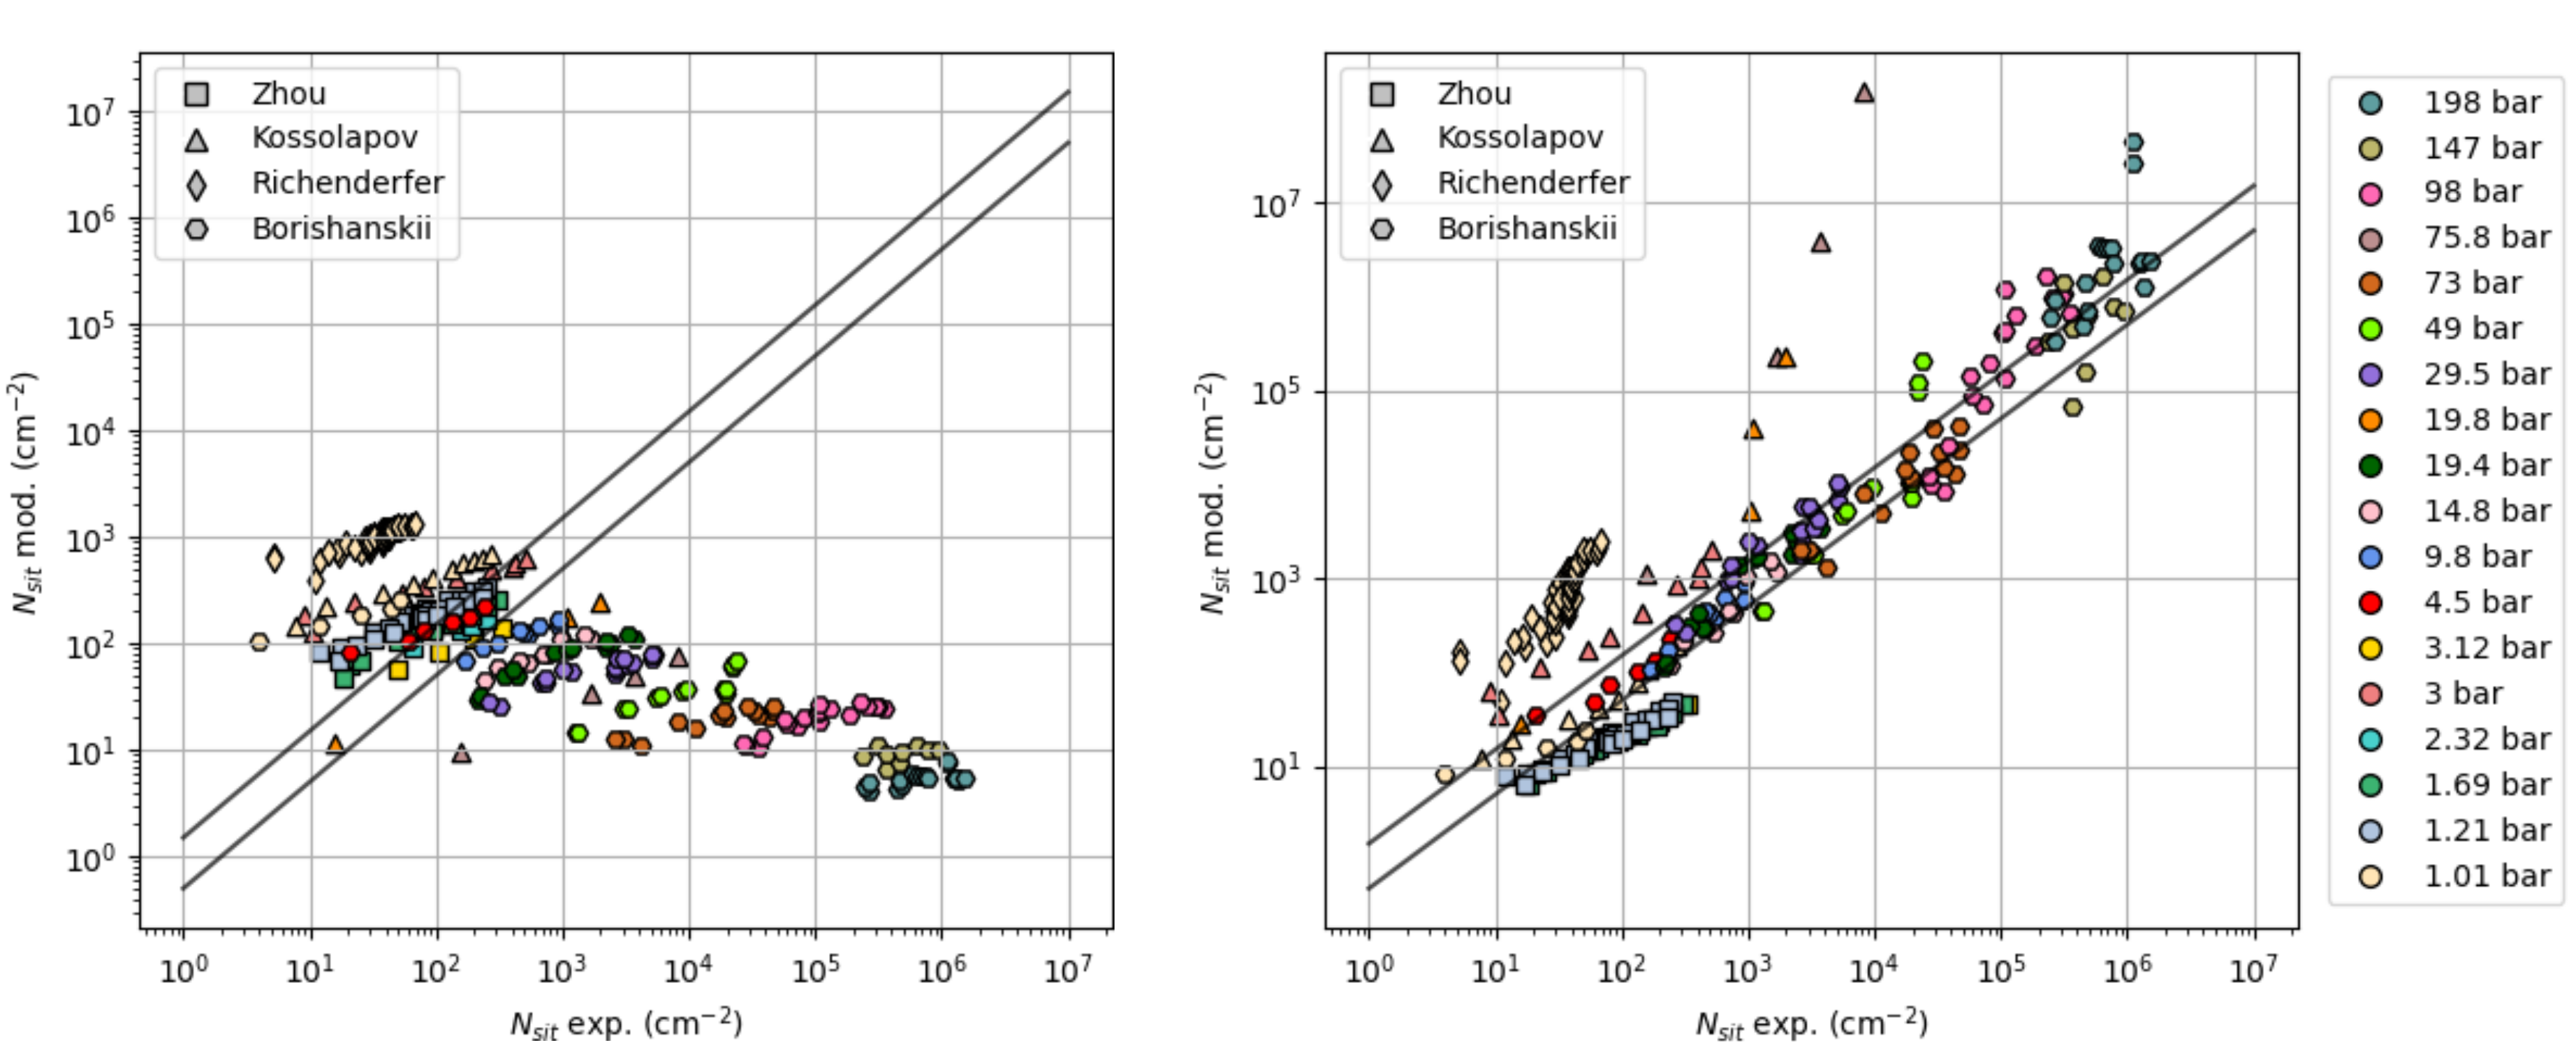
\includegraphics[scale=0.45]{img/DEBORA/nsit.png}
\caption{$N_{sit}$ correlations of {Lemmert} \& {Chawla} (left) and {Hibiki} \& {Ishii} (right) vs. exp. data from literature. Operation pressures are displayed. $\pm 50\%$ error bars are drawn in black.}
\label{fig:nsit}
\end{figure}
%

Figure \ref{fig:nsit} clearly shows that the {Lemmert} \& {Chawla} law lack of pressure dependence fails to reproduce high pressure measurements contrary to the {Hibiki} \& {Ishii} one. Even though {Hibiki} \& {Ishii} correlation shows significant discrepancies with measurements of {Kossolapov} \etal and {Richenderfer} \etal, its prediction capability is greater in average than {Lemmert} \& {Chawla} correlation.

%
\begin{figure}[h!]
\centering
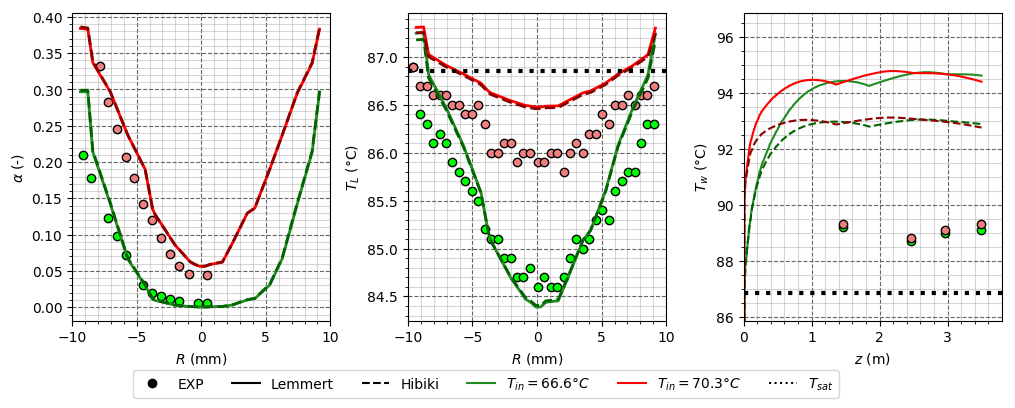
\includegraphics[scale=0.60]{img/DEBORA/plot_HI.png}
\caption{NCFD results for $\alpha$, $T_{L}$ and $T_{w}$ using {Lemmert} \& {Chawla} and {Hibiki} \& {Ishii} correlation. Cases 8G2P26W23Te66.6 and Te70.3, 30G2P26W23Te66.6 and 70.6.}
\label{fig:NCFD_nsit}
\end{figure}
%
To assess the influence of nucleation site density law on NEPTUNE\_CFD computations, we compare results obtained with both correlations on Figure \ref{fig:NCFD_nsit}, which shows a remarkable impact of the modification of $N_{sit}$ correlation. Using {Hibiki} \& {Ishii} correlation reduces the error on $T_{w}$ by approximately $2\degree\text{C}$ while $\alpha$ and $T_{L}$ remain unchanged. This implies that the same heat flux partitioning is found with the two models, but that the pressure dependence of {Hibiki} \& {Ishii} law helped to balance Equation \ref{eq:HFP} using a lower $T_{w}$, thus closer to experimental measurements.

Such a result indicates that the HFP model could be improved through a systematic analysis of each parameter's impact and modeling (bubble departure diameter, detachment frequency, etc.). Assembling a more recent and consistent model could provide better results regarding wall temperature prediction. Models such as the one developed by {Kommajosyula}\cite {Kommajosyula2020} could be interesting to apply for high-pressure flows.


Now that simple tube boiling flow has been assessed through the presented results, next section will focus on the simulation of boiling flow in a tube equipped with a mixing device.% using DEBORA-Promoteur experimental results.


\chapter{NEPTUNE\_CFD Simulations of DEBORA Cases}
\label{chap:debora_ncfd}

\minitoc

\section{Introduction}

Due to the large amount of measurements along with its scaling conditions with PWR flows, the DEBORA cases have been often used for validation of multiphase simulation tools, from simple 1D / 2D codes \cite{kledy_DEBORA, gueguen_contribution_2013, manon_contribution_2000} to CFD softwares \cite{mimouni_debora, guelfi_neptune, bestion_debora, baglietto_debora, montout}, helping to conduct separate validation and comparison of several modeling aspects involved in such codes (interfacial heat and momentum transfer, turbulence, interfacial area transport, etc.). 

\npar

In this Chapter, we present neptune\_cfd simulations of the DEBORA experiment. The objective is to assess the current modeling of the code for dispersed two-phase boiling flows. To do so, we will simulate cases from the different campaigns of the DEBORA database (C800 and C3000) to conduct comparisons of void faction, bubble diameter, vapor velocity, liquid temperature and wall temperature profiles.

\npar

As identified in Chapter \ref{chap:debora}, our focus will be on cases from the G2P26W16 series, since they provide the most extensive set of measurements in very close operating conditions.


\section{Simulation Setup}

Since the geometry of the DEBORA experiment presents an axisymmetry, we simplify the simulation setup in order to realize a 2D axisymmetric computation. The computational domain consists of a 1$\degree$ angular section of radius $R=9.6$\ mm and 3.85\ m length (Figure \ref{fig:deb_cfd_domain}).


\begin{figure}[!h]
\centering
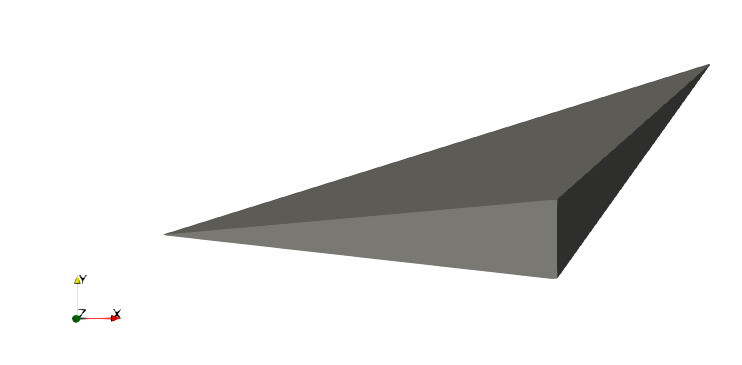
\includegraphics[width=0.6\linewidth]{img/DEBORA/cfd/msh/domain.png}
\caption{View of the computational domain.}
\label{fig:deb_cfd_domain}
\end{figure}


The boundary conditions are:

\begin{itemize}
\item Uniform heat flux for $0.2$\ m $\leq z \leq$ 3.5\ m ;
\item Adiabatic wall for $z<0.2$\ m and $z>3.7$\ m ;
\item Uniform outlet pressure ;
\item Uniform liquid inlet velocity and temperature ;
\item Symmetry condition on remaining faces.
\end{itemize}

The inlet section before heating is approximately $10D_{h}$ long and the extracted radial profile for comparisons is located at the end of the heating length. The angular section consists of 1 mesh while radial and axial direction are uniformly discretized. Four meshes are considered, presented on Table \ref{tab:deb_cfd_msh} and Figure \ref{fig:deb_cfd_msh_rad}.



\begin{table}[!h]
\centering

\begin{tabular}{c||c|c|c|c}
Mesh name & M1 & M2 & M4 & M8  \\
\hline
Number of cells (radial $\times$ axial) & 10  $\times$ 100 & 20 $\times$ 200 & 40 $\times$ 400 & 80 $\times$ 800
\end{tabular}

\caption{Mesh parameters}
\label{tab:deb_cfd_msh}

\end{table}

\npar

\begin{figure}[!h]
\centering
\subfloat[Mesh M1]{
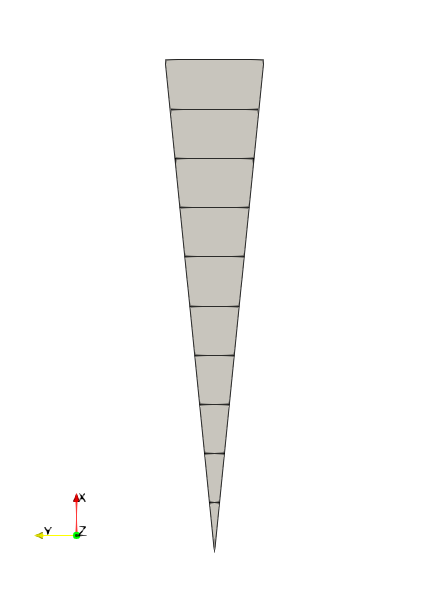
\includegraphics[width=0.25\linewidth]{img/DEBORA/cfd/msh/deb_m1.png}
}
\subfloat[Mesh M2]{
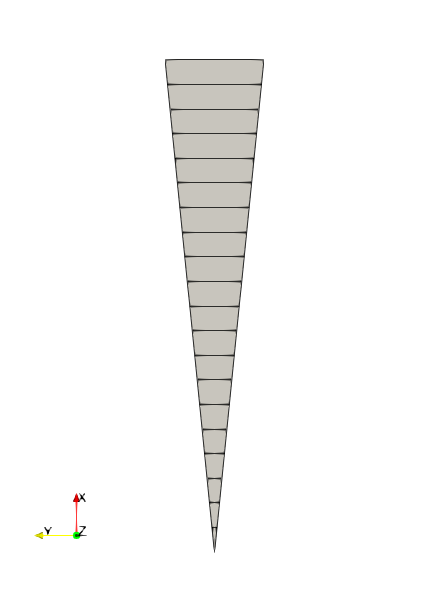
\includegraphics[width=0.25\linewidth]{img/DEBORA/cfd/msh/deb_m2.png}
}
\subfloat[Mesh M4]{
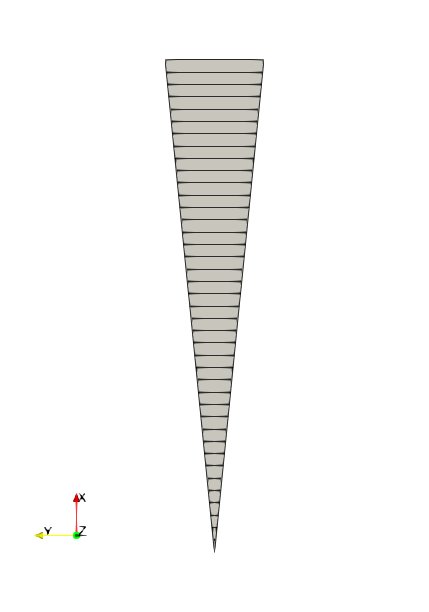
\includegraphics[width=0.25\linewidth]{img/DEBORA/cfd/msh/deb_m4.png}
}
\subfloat[Mesh M8]{
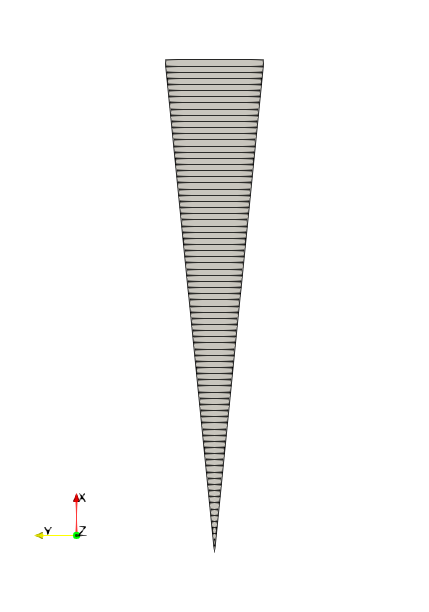
\includegraphics[width=0.25\linewidth]{img/DEBORA/cfd/msh/deb_m8.png}
}
\caption{View of the radial meshes.}
\label{fig:deb_cfd_msh_rad}
\end{figure}


\npar

The computation runs using the transient solver of NCFD for a long enough physical time ensuring temporal stabilization and convergence of the results. 

\begin{note*}{}
First simulated case was simulated up to a physical time of 40\ s, ensuring the time-convergence. Further simulations used this first case as a restart point, allowing to reach time-convergence in less than 10\ s when changing boundary conditions.  
\end{note*}



\section{Mesh Sensitivity Study}

On Figure \ref{fig:deb_cfd_msh_sensi}, we present simulation results for the 4 meshes (Table \ref{tab:deb_cfd_msh}) of the case 30G2P26W16Te66.6. 

\begin{figure}[!h]
\centering
\subfloat[Void fraction]{
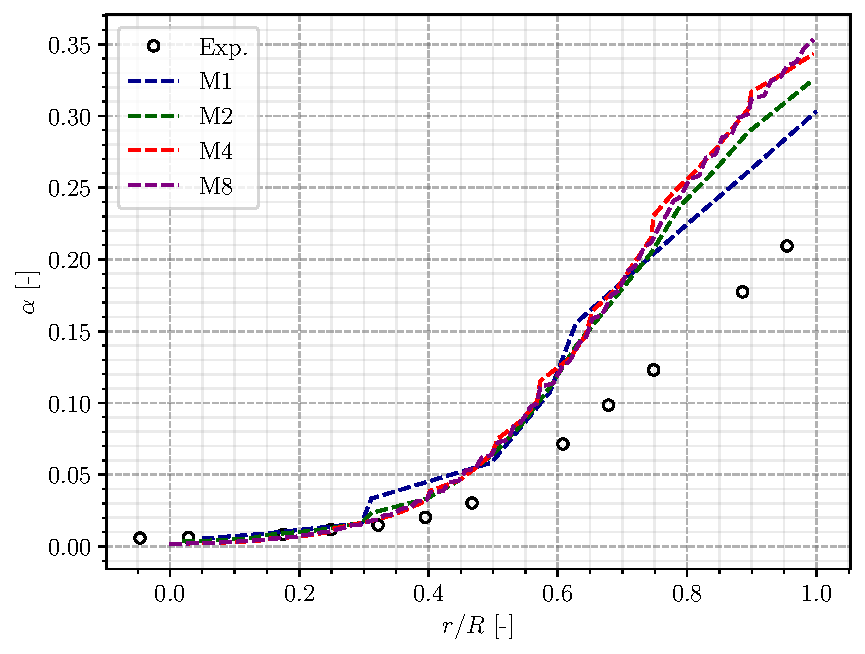
\includegraphics[width=0.4\linewidth]{img/DEBORA/cfd/30G2P26W16/30T66_alpha_msh.pdf}
}
\subfloat[Bubble diameter]{
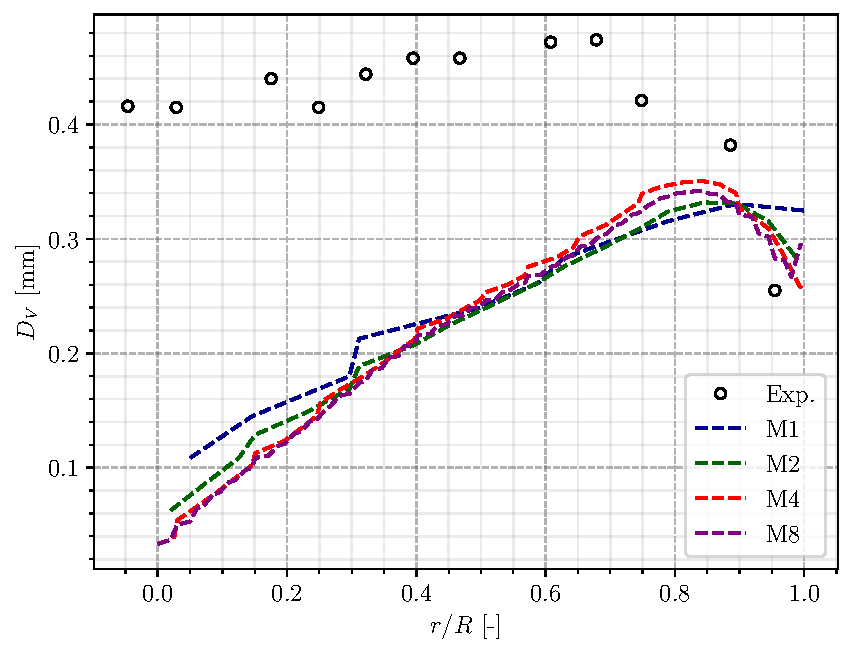
\includegraphics[width=0.4\linewidth]{img/DEBORA/cfd/30G2P26W16/30T66_dV_msh.pdf}
}
\\
\subfloat[Vapor velocity]{
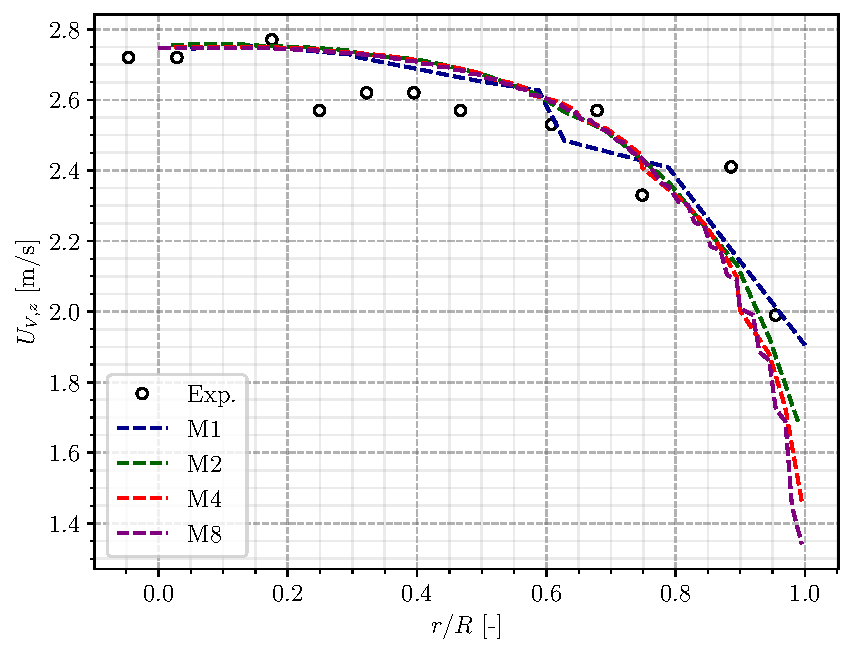
\includegraphics[width=0.4\linewidth]{img/DEBORA/cfd/30G2P26W16/30T66_Uvap_msh.pdf}
}
\subfloat[Liquid temperature]{
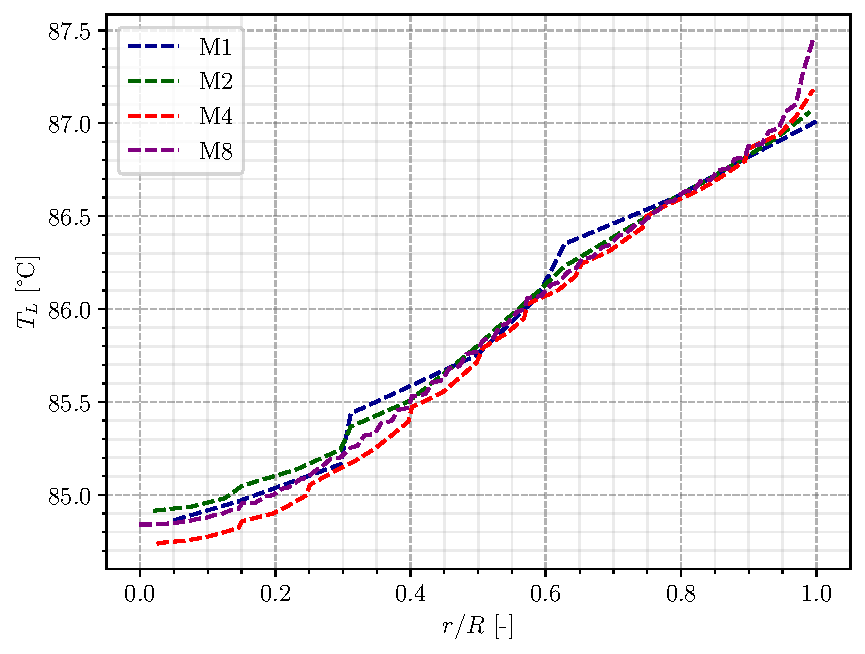
\includegraphics[width=0.4\linewidth]{img/DEBORA/cfd/30G2P26W16/30T66_TL_msh.pdf}
}
\caption{Mesh sensitivity study for 30G2P26Te66.6 case}
\label{fig:deb_cfd_msh_sensi}
\end{figure}


We see that the different meshes provide similar results for the void fraction, bubble diameter, vapor velocity and liquid temperature. This is particularly true for the M4 and M8 meshes, allowing to assume that an acceptable grid convergence is reached with the M4 mesh. \textbf{Therefore, further simulations will be conducted using the M4 mesh.}

\begin{remark*}
One of the most remarkable impact of the mesh concerns the liquid temperature in the wall-adjacent cell. As the mesh refines, the strong temperature gradient at the wall is logically better captured, inducing a net rise in the liquid temperature when $r/R \to 1$.
\end{remark*}



\section{C800 Cases Simulations : Thermal Measurements}

In this Section, we focus our attention on cases from the 8G2P26W16 series to assess liquid and wall temperature predictions. We sub-divide the case in three parts depending on the degree of subcooling at the outlet in order to cover both single-phase and fully boiling cases.



\subsection{High Subcooling Cases}

We start by simulating cases 8G2P26W16Te31.5 and Te44.9 which both have an outlet quality $x_{eq,out}<-0.25$, meaning that the fluid remains in its liquid phase along nearly the entire heating length. Results obtained for those cases are presented on Figure \ref{fig:deb_cfd_8T33_T44}.

\begin{figure}[!h]
\centering
\subfloat[Liquid temperature]{
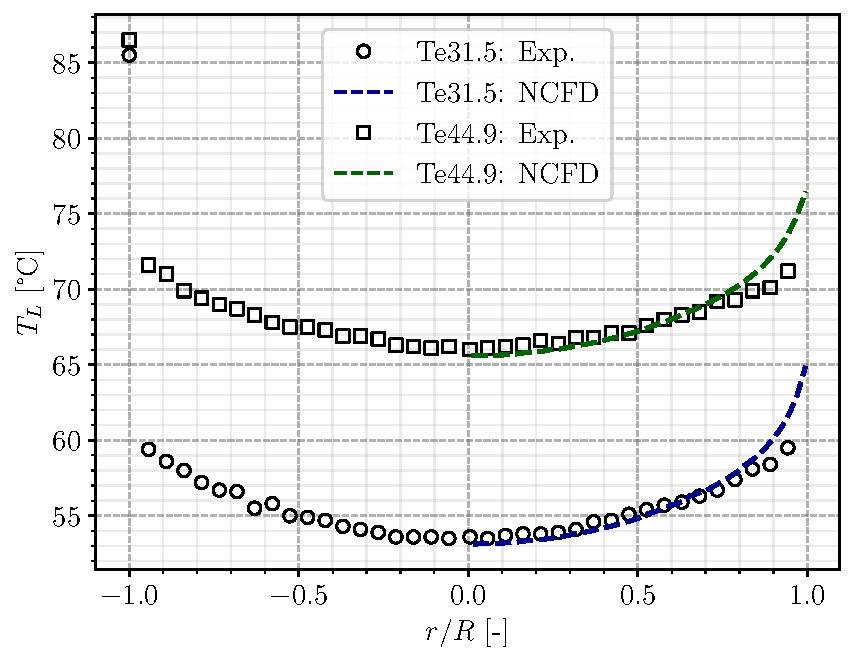
\includegraphics[width=0.4\linewidth]{img/DEBORA/cfd/8G2P26W16/8T31_T44_TL_ref.pdf}
\label{fig:8T31_T44_TL}
}
\subfloat[Wall temperature vs. axial position]{
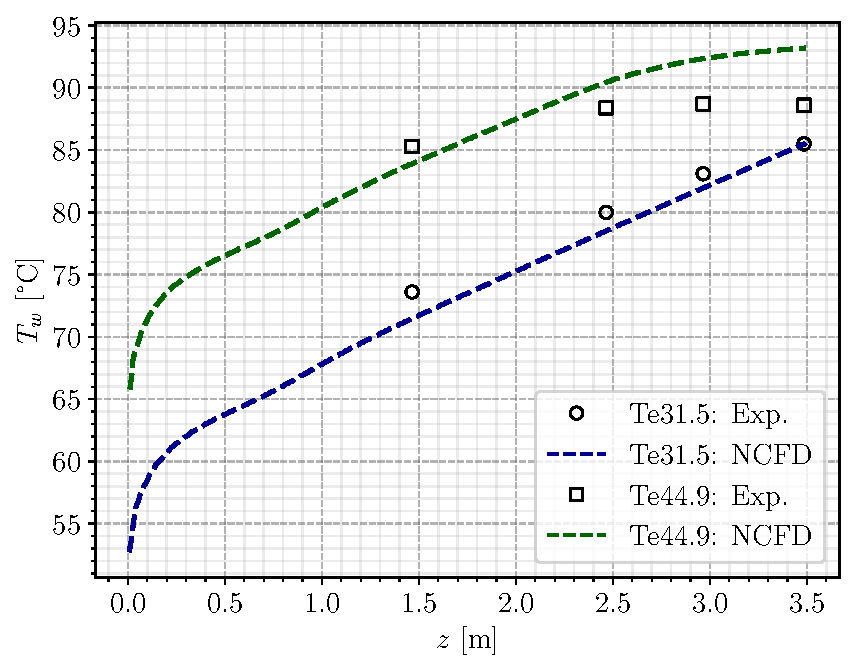
\includegraphics[width=0.4\linewidth]{img/DEBORA/cfd/8G2P26W16/8T31_T44_Tw_ref.pdf}
\label{fig:8T31_T44_Tw}
}
\\
\subfloat[Wall temperature vs. local quality]{
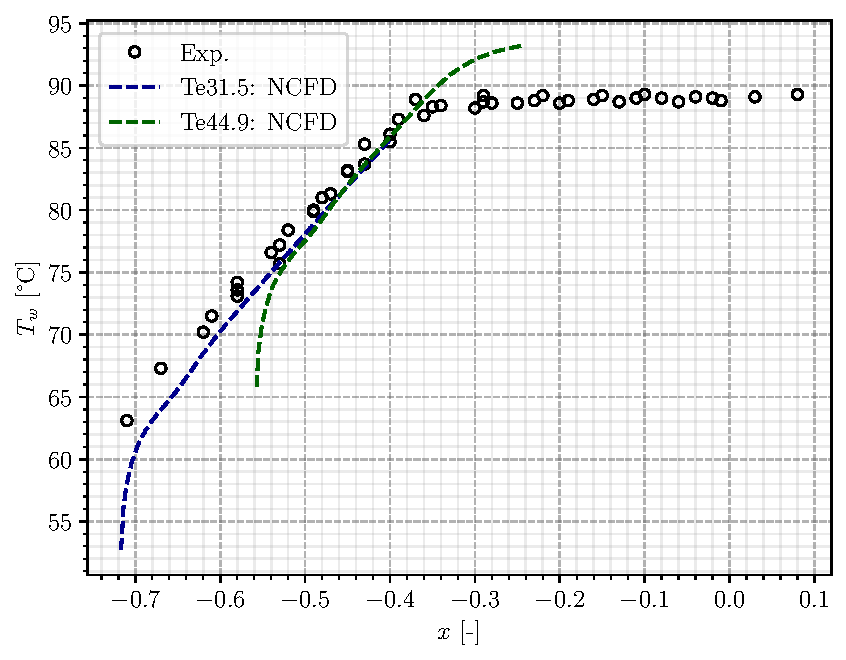
\includegraphics[width=0.4\linewidth]{img/DEBORA/cfd/8G2P26W16/8T31_T44_Tw_x_ref.pdf}
\label{fig:8T31_T44_Tw_x}
}
\caption{Simulation results for cases 8G2P26W16Te31. 5\& Te44.9}
\label{fig:deb_cfd_8T33_T44}
\end{figure}

\npar

The liquid temperature profiles are fairly reproduced with experimental the parabolic shape correctly captured along with quite precise prediction of the temperature values in the bulk (Figure \ref{fig:8T31_T44_TL}). Still, we note that an overestimation near the wall and a small underestimation (less than $1\degC$) when approaching the center of the pipe.

\npar

Wall temperature predictions in the single-phase region present a good agreement with the experimental measurements along the axial positions (Figure \ref{fig:8T31_T44_Tw}). This is further verified by transposition along the local quality $x_{eq}$ (Figure \ref{fig:8T31_T44_Tw_x}) gathering all the measurements from the 8G2P26W16 campaign, showing an average error of approximately $1 \degC$ up to $x_{eq} \approx -0.5$.

\npar

Those comparisons highlight the validation of the code for the single-phase flow part, implying that \textbf{the local liquid heat transfer coefficient (Eq. \ref{eq:ncfd_hfc}) is correctly computed along with a good heat transport along the radial direction}.


\subsection{Low Subcooling Cases}

Next cases to be simulated are 8G2P26W16Te55.7 and Te61.5. Their outlet quality is closer to saturation with $x_{eq,out} \geq -0.1$ and thus present a subcooled boiling region during a significant portion of the heating length. However, the bulk flow is expected to stay fully liquid in those conditions (Figure \ref{fig:G2P26W16_alpha}). The results are presented of Figure \ref{fig:deb_cfd_8T55_T61}.


\begin{figure}[!h]
\centering
\subfloat[Liquid temperature]{
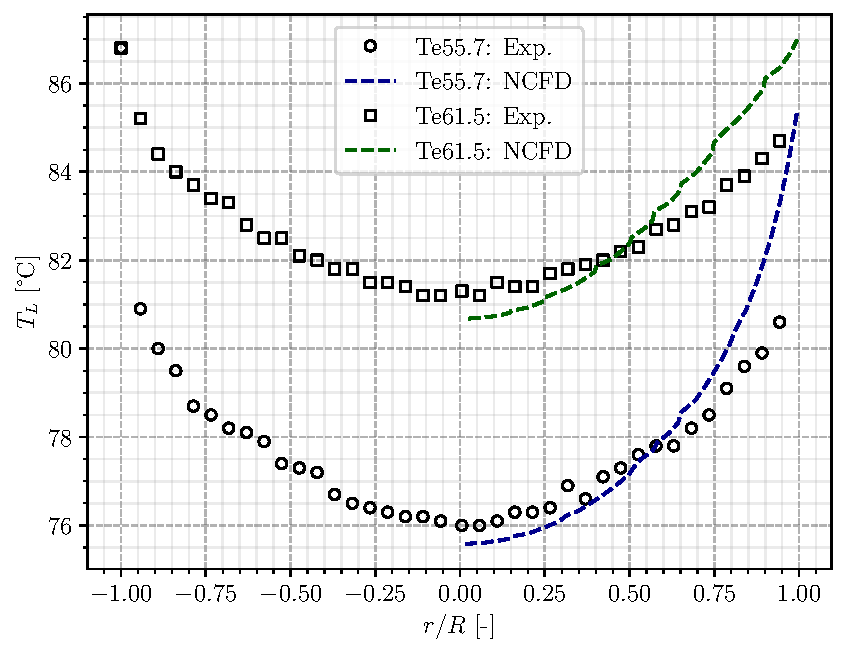
\includegraphics[width=0.4\linewidth]{img/DEBORA/cfd/8G2P26W16/8T55_T61_TL_ref.pdf}
\label{fig:8T55_T61_TL}
}
\subfloat[Wall temperature vs. axial position]{
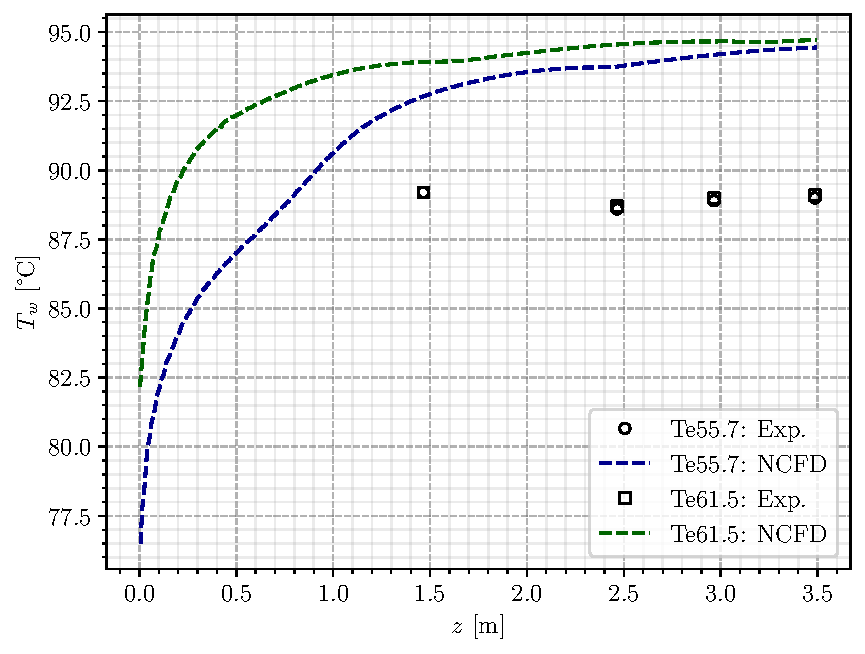
\includegraphics[width=0.4\linewidth]{img/DEBORA/cfd/8G2P26W16/8T55_T61_Tw_ref.pdf}
\label{fig:8T55_T61_Tw}
}
\\
\subfloat[Wall temperature vs. local quality]{
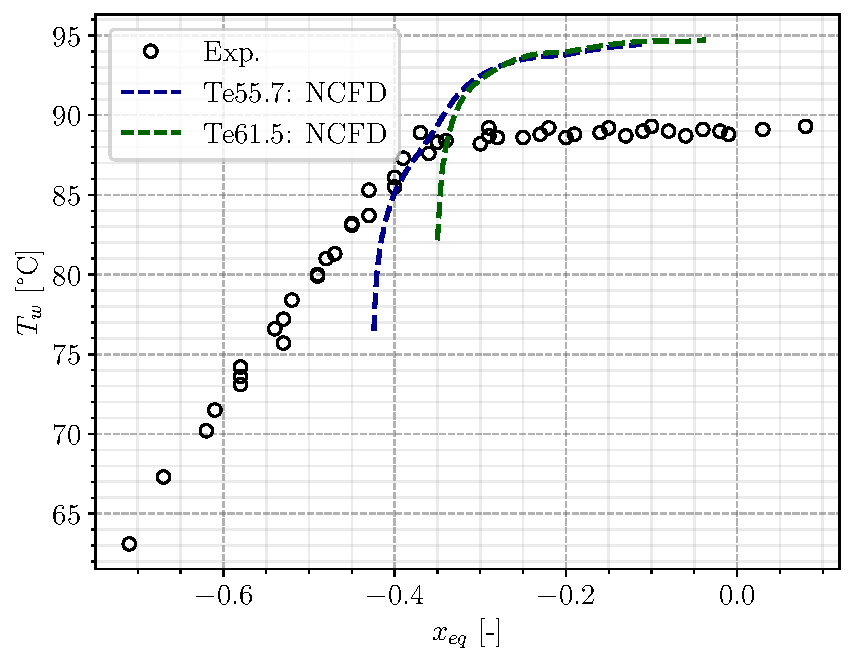
\includegraphics[width=0.4\linewidth]{img/DEBORA/cfd/8G2P26W16/8T55_T61_Tw_x_ref.pdf}
\label{fig:8T55_T61_Tw_x}
}
\caption{Simulation results for cases 8G2P26W16Te55.7 \& Te61.5}
\label{fig:deb_cfd_8T55_T61}
\end{figure}

\npar

Liquid temperature profiles (Figure \ref{fig:8T55_T61_TL}) are similar to those of the high subcooling cases (Figure \ref{fig:8T31_T44_TL}). The parabolic shape of the measurements is reasonably reproduced, with liquid temperature values close to the experiment. The same discrepancies are observed, namely a overestimation close to the wall and a small underestimation at the center (also lower than $1\degC$).

\npar

However, the wall temperature start to show significant discrepancies with the measurements (Figure \ref{fig:8T55_T61_Tw}). The deviation from the linear profile observed in the pure-single phase region towards a stabilization corresponding to the boiling regime fails to be reproduced (Figure \ref{fig:8T55_T61_Tw_x}). First, the temperature plateau appears to start later than the experiment (around $x_{eq}\approx -0.3$ for the simulations contrary to $x_{eq} \approx -0.4$ for the experiments) and further reaches a wall temperature up to $6 \degC$ above the measurements.

\npar
Albeit the liquid temperature seems correctly distributed along the radial direction in the subcooled boiling region (also meaning that any amount of vapor potentially produced at the wall is correctly re-condensed), the wall temperature behavior significantly deviates from the experiments both by missing the ONB and exhibiting a too large superheat in the boiling region. \textbf{This consequently casts interrogations towards the modeling of the wall temperature in the code, which is a result of the wall boiling model (Section \ref{sec:ncfd_HFP}).}



\subsection{Saturated Cases}

Finally, we focus on saturated cases 8G2P26W16Te66.6 and Te70.3, both having an outlet quality $x_{eq,out} > 0$. Under those operating conditions, uncondensed vapor is present in the bulk flow (Figure \ref{fig:G2P26W16_alpha}). Results of the simulation sfor those cases are presented on Figure \ref{fig:deb_cfd_8T66_T70}.



\begin{figure}[!h]
\centering
\subfloat[Liquid temperature]{
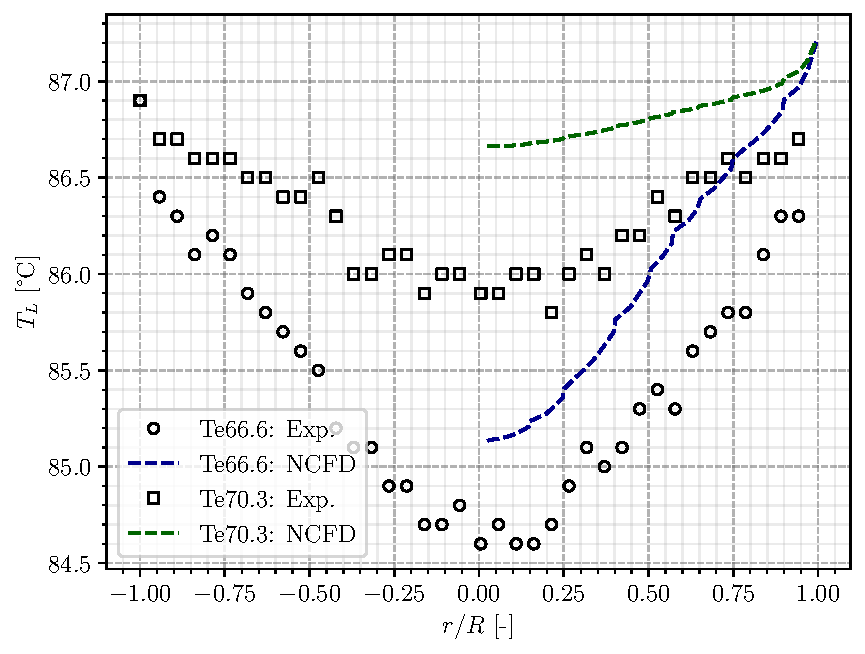
\includegraphics[width=0.4\linewidth]{img/DEBORA/cfd/8G2P26W16/8T66_T70_TL_ref.pdf}
\label{fig:8T66_T70_TL}
}
\subfloat[Wall temperature vs. axial position]{
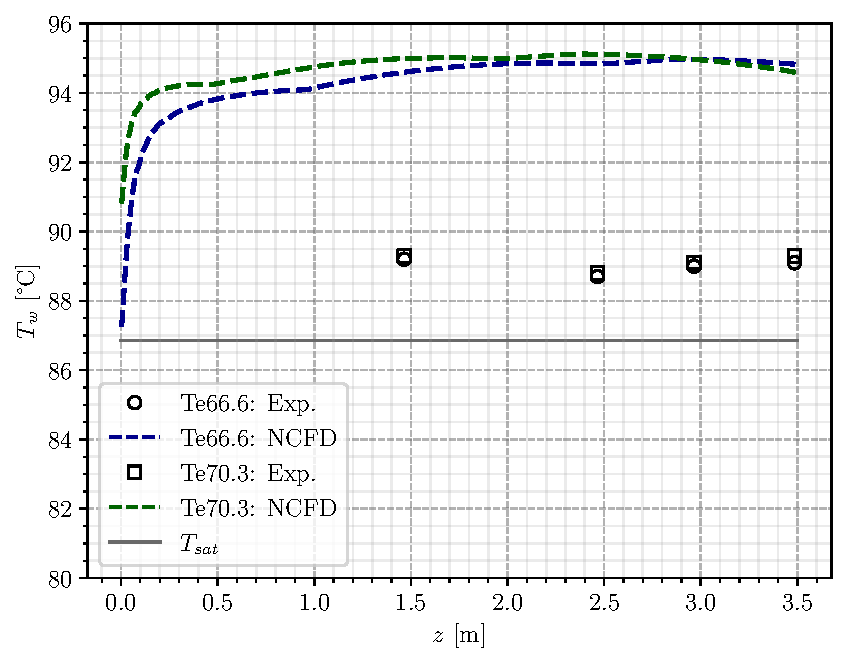
\includegraphics[width=0.4\linewidth]{img/DEBORA/cfd/8G2P26W16/8T66_T70_Tw_ref.pdf}
\label{fig:8T66_T70_Tw}
}
\\
\subfloat[Wall temperature vs. local quality]{
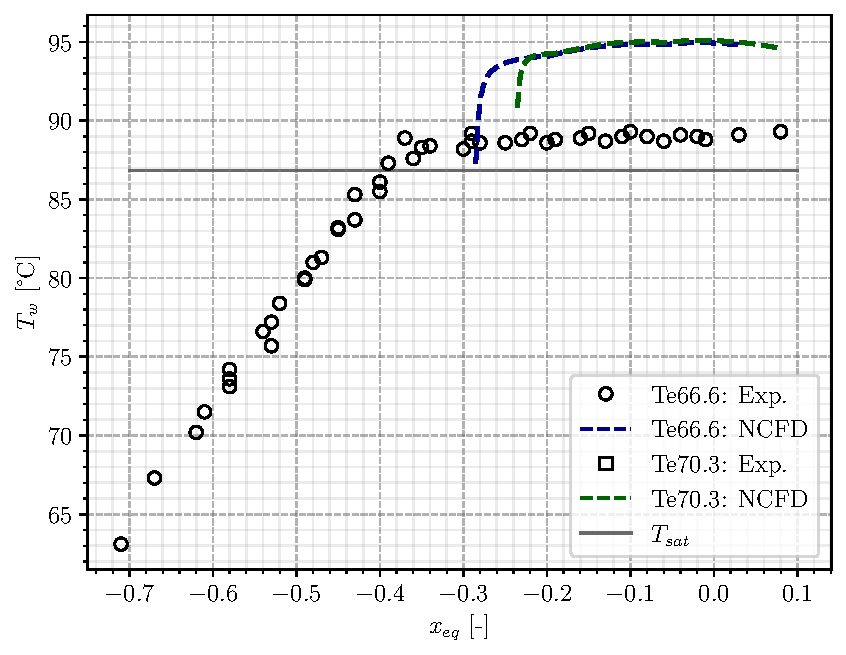
\includegraphics[width=0.4\linewidth]{img/DEBORA/cfd/8G2P26W16/8T66_T70_Tw_x_ref.pdf}
\label{fig:8T66_T70_Tw_x}
}
\caption{Simulation results for cases 8G2P26W16Te66.6 \& Te70.3}
\label{fig:deb_cfd_8T66_T70}
\end{figure}


Contrary to previous observations in subcooled cases, the liquid temperature profiles (Figure \ref{fig:8T66_T70_TL}) are are overestimated ($\approx +0.6\degC$) over the whole radial section for both cases. The shape exhibited are however similar to the experiments, with a flattening of the liquid temperature for the Te70.3 case.

\npar

In those conditions, boiling starts immediately at the beginning of the heated length. Therefore, wall temperature is expected to rapidly stabilize to the boiling temperature, which is actually what happens in the simulations (Figure \ref{fig:8T66_T70_Tw})). As previously noted for the low subcooling cases, the wall temperature during boiling is overestimated by approximately $6\degC$. 

\npar

Those saturated cases are confirming that \textbf{the boiling model fails to predict the wall temperature}. 


\begin{remark*}{}
The small yet observed global overestimation of the liquid temperature may be a consequence of a either a too large condensation or interfacial area concentration (\ie small bubble diameter). 
\end{remark*}




\section{C3000 Cases Simulations : Topology Measurements}

Now that comparisons with thermal measurements have been conducted, we move to assessment of core flow topology predictions by the code. Based on results from the 30G2P26W16 campaign, we will compare the predictions of the void fraction, the bubble diameter and the vapor velocity at the end of the heating length. We will separately focus on subcooled boiling and saturated cases.


\subsection{Subcooled Boiling Cases}

Subcooled cases 30G2P26W16Te62 and Te64 are simulated. They both have an outlet quality $x_{eq,out} \leq 0$ with pure liquid at the center of the test section, but present significant void fraction when approaching the wall (Figure \ref{fig:G2P26W16_alpha}). Results of the NEPTUNE\_CFD Simulations are presented on Figure \ref{fig:deb_cfd_30T66_T70}.

\begin{figure}[!h]
\centering
\subfloat[Void fraction]{
\includegraphics[width=0.4\linewidth]{img/DEBORA/cfd/30G2P26W16/30T62_T64_alpha_ref.pdf}
\label{fig:30T62_T64_alpha}
}
\subfloat[Bubble diameter]{
\includegraphics[width=0.4\linewidth]{img/DEBORA/cfd/30G2P26W16/30T62_T64_dV_ref.pdf}
\label{fig:30T62_T64_dV}
}
\\
\subfloat[Vapor velocity]{
\includegraphics[width=0.4\linewidth]{img/DEBORA/cfd/30G2P26W16/30T62_T64_Uvap_ref.pdf}
\label{fig:30T62_T64_Uvap}
}
\caption{Simulation results for cases 30G2P26W16Te62 \& Te64}
\label{fig:deb_cfd_30T62_T64}
\end{figure}


\npar

The void fraction (Figure \ref{fig:30T62_T64_alpha}) appears globally overestimated over the whole radial section, with a difference $\alpha_{CFD} - \alpha_{exp} \approx 10\%$ at the wall. However the results seem to match the very low void fractions region ($\alpha < 3\%$) and finds a pure liquid flow roughly at the same radial position as the measurements ($r/R \approx 0.5$ and $0.3$ for Te62 and Te64 cases respectively).

\npar

On the other hand, the bubble diameter (Figure \ref{fig:30T62_T64_dV}) is largely underestimated by vanishing rapidly when $r/R < 0.9$ which is not observed experimentally. Measurements contrarily show a roughly constant bubble diameter after a small increase. The simulations yet present an acceptable agreement with the experiments near the wall and even present a slight growth of the bubble diameter before its immediate decrease. \textbf{Such a discrepancy combined to a too large void fraction points towards an erroneous estimation of bubble break-up and / or condensation.}

\npar

The vapor velocity profiles (Figure \ref{fig:30T62_T64_Uvap}) are in accordance with the DEBORA measurements, both in the values and profile shape. \textbf{This may be supporting the evaluation of the interfacial momentum transfer determining the drift velocity between liquid and vapor.}


\subsection{Saturated Boiling Cases}

Next we simulate two saturated cases that experimentally present a non-zero void fraction at the tube center : cases 30G2P26W16Te66 and Te70. Results are presented of Figure \ref{fig:deb_cfd_30T66_T70}.

\begin{figure}[!h]
\centering
\subfloat[Void fraction]{
\includegraphics[width=0.4\linewidth]{img/DEBORA/cfd/30G2P26W16/30T66_T70_alpha_ref.pdf}
\label{fig:30T66_T70_alpha}
}
\subfloat[Bubble diameter]{
\includegraphics[width=0.4\linewidth]{img/DEBORA/cfd/30G2P26W16/30T66_T70_dV_ref.pdf}
\label{fig:30T66_T70_dV}
}
\\
\subfloat[Vapor velocity]{
\includegraphics[width=0.4\linewidth]{img/DEBORA/cfd/30G2P26W16/30T66_T70_Uvap_ref.pdf}
\label{fig:30T66_T70_Uvap}
}
\caption{Simulation results for cases 30G2P26W16Te66 \& Te70}
\label{fig:deb_cfd_30T66_T70}
\end{figure}

Similar to the subcooled cases, the void fraction (Figure \ref{fig:30T66_T70_alpha}) is overestimated over the whole section. Case Te66 presents a wall overestimation of approximately 10\% as for the subcooled simulations (Figure \ref{fig:30T62_T64_alpha})and matches the radial position where $\alpha \approx 0$. On the contrary, case Te70 is largely overestimated over the whole section, which can be explained because the liquid temperature is close to saturation, strongly limiting the impact of condensation.

\npar

Bubble diameter (Figure \ref{fig:30T66_T70_dV}) for the Te66 case behaves close to the subcooled cases, with a large overestimation under the sharp decrease when $r/R < 0.8$. However, case Te70 presents a a different profile with a larger growth in bubble diameter nearly matching maximum experimental value at $r/R \approx 0.6$, but then decreases too rapidly. Recalling thermal results for the 8G2P26W16Te70.3 case presenting similar operating conditions (Figure \ref{fig:8T66_T70_TL}), $r/R \approx 0.6$ corresponds to the radial position where the computed liquid temperature becomes lower than saturation temperature, enabling condensation to occur. This tends to indicate that \textbf{condensation may be responsible for most of the bubble diameter underestimation in the sub-cooled region}. On the contrary, \textbf{coalescence and break-up terms alone seem to be able to reproduce the bubble diameter increase before condensation starts}.

\npar

Finally, vapor velocity (Figure \ref{fig:30T66_T70_Uvap}) is correctly reproduced for the Te66 case while the Te70 simulation do not reproduce the plateau observed in the measurements by keeping a parabolic profile from which the experiment deviates. The velocity magnitude achieved for the Te70 case are however coherent with the experiments. 


\section{Simulations Sensitivity Tests}


\subsection{Sensitivity to Wall Heat Flux Correction}


%%



%\subsection{Sensitivity to Condensation and Bubble Break-Up}
%
%Some sensitivity to Break-Up term and Condensation term if relevant


\subsection{Influence of a Wall Boiling Parameter : the Nucleation Site Density}

Comparison between Lemmert, Hibiki and Li

Show HFP along the tube --> impact on flux partition but not at bulk --> too large influence of condensation and interfacial area.

--> Need for a new HFP model, including new laws. 



\section{Conclusion}

\clearpage









In this work, we present the simulations of the following cases:
\begin{itemize}
\item C8G2P26W16Te44.9 and C8G2P26W16Te49.6 (single-phase flow)
\item C8G2P26W16Te66.6 and C8G2P26W16Te70.3 (two-phase flow)
\item C30G2P26W16Te66.6 and C30G2P26W16Te70.6 (two-phase flow)
\end{itemize}

The pressure of $26~\text{bar}$ is chosen to match the pressure of the mixing vanes cases (DEBORA-Promoteur, Section \ref{sec:deb_prom}). Mesh sensitivity is performed over two meshes: a large mesh (M1) with $460~356\text{ cells }=338\text{ radial } \times 1362 \text{ axial cells}$ and a fine mesh (M2) with $3~157~952\text{ cells }=1568\text{ radial } \times 2014 \text{ axial cells}$.

On Figure \ref{fig:th_1phi_res}, we present the results regarding liquid temperature at the outlet and wall temperature. The liquid temperature profile seems to be correctly reproduced by the simulations, though we see a slight overestimation close to the wall. Looking closer at boiling cases shows a difference of $\approx 0.5\degree$ C, which is close to the uncertainty of the measurements \cite{garnier_local_2001}. Concerning the wall temperature, it appears that it is underestimated before the \textbf{Onset of Nucleate Boiling} (ONB) ($T_{w}<T_{sat}$) and overestimated after the ONB ($\approx +5\degree$C). Post-ONB wall temperature is characterized by a stabilization of its value above the saturation temperature (here $T_{w,ONB}-T_{sat}\approx 2\degree\text{C}$).

%
\begin{figure}[h!]
\centering
\includegraphics[scale=0.60]{img/DEBORA/c8.png}
\caption{NCFD (lines) vs. Exp. (circles) - $T_{L}$ and $T_{w}$ - Cases C8G2P26W16Te44.9, Te49.6, Te66.6 and Te70.3 - Simulations using two meshes M1 (coarse) and M2 (fine).}
\label{fig:th_1phi_res}
\end{figure}
%

%%
%\begin{figure}[!htb]
%\vspace{16pt}
%\begin{spacing}{1.0}
%\centering
%\includegraphics[scale=0.60]{img/DEBORA/thermal_diph.png}
%\caption{NEPTUNE\_CFD simulations results vs. experimental measurements - $T_{L}$ and $T_{w}$ - Cases C8G2P26W16Te66.6 and C8G2P26W16Te70.3}
%\label{fig:th_diph_res}
%\end{spacing}
%\vspace{16pt}
%\end{figure}
%%



%
\begin{figure}[h!]
\centering
\includegraphics[scale=0.60]{img/DEBORA/c30.png}
\caption{NCFD (lines) vs. Exp. (circles) - $\alpha$, $d_{G}$ and $U_{G,z}$ - Cases C30G2P26W16Te66.6 and Te70.6 - Simulations using two meshes M1 (coarse) and M2 (fine).}
\label{fig:topology_res}
\end{figure}
%

On Figure \ref{fig:topology_res}, we compare the results of the simulations to the experiments regarding void fraction, bubble Sauter diameter and axial gas velocity. Void fraction profiles are quite correctly reproduced, though we observe a $10\%$ higher peak at the wall for $T_{in}=66.6\degree$C. The order of magnitude of bubble diameter is correct ($\sim 0.1\text{mm}$) and NEPTUNE\_CFD manages to detect coalescence (increase of bubble diameter when leaving the wall) and bulk condensation (decrease of bubble diameter when reaching the core of the flow), which is in qualitative agreement with the experiments. Quantitatively speaking, bubble diameter is globally underestimated. Finally, gas velocity profile is reasonably reproduced for $T_{in}=66.6\degree$C, but not for $T_{in}=70.6\degree$C. The latter experimental profile is flatter, which could be explained by a change of flow regime since uncondensed vapor is detected in the bulk.  

Finally, the simulations reasonably agree with the experiments. The strongest discrepancies being mostly the wall temperature and bubble diameter. Potential ways of improving those results are investigated in next sub-section.

\subsection{Investigating the nucleation site density modeling $N_{sit}$}

In NEPTUNE\_CFD, wall temperature is computed through the Heat Flux Partitioning model, which role is to find the appropriate $T_{w}$ which balances Equation $\ref{eq:HFP}$. However, some laws used to express parameters such as $N_{sit}$, $f$, or $d_{d}$ are quite old and simple. For instance, the {Lemmert} \& {Chawla}\cite{lemmert_influence_1977} expression of $N_{sit}$ only depends on the wall superheat (Sub-section \ref{subsec:HFP}).%, meaning that it can not reproduce potential influence of the pressure on the nucleation site density.

A comparison of the {Lemmert} \& {Chawla} law\cite{lemmert_influence_1977} with  the {Hibiki} \& {Ishii}\cite{hibiki_active_2003} law for $N_{sit}$ against 4 data sets from the literature is presentend on Figure \ref{fig:nsit}. The {Hibiki} \& {Ishii} correlation depends simultaneously on wall superheat, pressure and contact angle.  Experimental measurements of {Borishanskii} \etal\cite{borishanskii_heat_1969}, {Richenderfer} \etal\cite{richenderfer_investigation_2018}, {Kossolapov} \etal\cite{kossolapov_experimental_2021} and {Zhou} \etal\cite{zhou_experimental_2020-1} are used to assess the two nucleation site density correlations.
%
\begin{figure}[h!]
\centering
\includegraphics[scale=0.45]{img/DEBORA/nsit.png}
\caption{$N_{sit}$ correlations of {Lemmert} \& {Chawla} (left) and {Hibiki} \& {Ishii} (right) vs. exp. data from literature. Operation pressures are displayed. $\pm 50\%$ error bars are drawn in black.}
\label{fig:nsit}
\end{figure}
%

Figure \ref{fig:nsit} clearly shows that the {Lemmert} \& {Chawla} law lack of pressure dependence fails to reproduce high pressure measurements contrary to the {Hibiki} \& {Ishii} one. Even though {Hibiki} \& {Ishii} correlation shows significant discrepancies with measurements of {Kossolapov} \etal and {Richenderfer} \etal, its prediction capability is greater in average than {Lemmert} \& {Chawla} correlation.

%
\begin{figure}[h!]
\centering
\includegraphics[scale=0.60]{img/DEBORA/plot_HI.png}
\caption{NCFD results for $\alpha$, $T_{L}$ and $T_{w}$ using {Lemmert} \& {Chawla} and {Hibiki} \& {Ishii} correlation. Cases 8G2P26W23Te66.6 and Te70.3, 30G2P26W23Te66.6 and 70.6.}
\label{fig:NCFD_nsit}
\end{figure}
%
To assess the influence of nucleation site density law on NEPTUNE\_CFD computations, we compare results obtained with both correlations on Figure \ref{fig:NCFD_nsit}, which shows a remarkable impact of the modification of $N_{sit}$ correlation. Using {Hibiki} \& {Ishii} correlation reduces the error on $T_{w}$ by approximately $2\degree\text{C}$ while $\alpha$ and $T_{L}$ remain unchanged. This implies that the same heat flux partitioning is found with the two models, but that the pressure dependence of {Hibiki} \& {Ishii} law helped to balance Equation \ref{eq:HFP} using a lower $T_{w}$, thus closer to experimental measurements.

Such a result indicates that the HFP model could be improved through a systematic analysis of each parameter's impact and modeling (bubble departure diameter, detachment frequency, etc.). Assembling a more recent and consistent model could provide better results regarding wall temperature prediction. Models such as the one developed by {Kommajosyula}\cite{kommajosyula_development_2020} could be interesting to apply for high-pressure flows.


Now that simple tube boiling flow has been assessed through the presented results, next section will focus on the simulation of boiling flow in a tube equipped with a mixing device.% using DEBORA-Promoteur experimental results.

\cleardoublepage % Empty page before the start of the next part


\part{Development of a New Wall Heat Flux Partitioning Model}


% Chapter X

\chapter{Existing Heat Flux Partitioning Models} % Chapter title

\label{ch:name} % For referencing the chapter elsewhere, use \autoref{ch:name} 

%----------------------------------------------------------------------------------------

\section{Kurul \& Podowski (1990)}


In their original work published in 1990, Kurul \& Podowski proposed a first complete closure for the wall heat flux partition.


\npar
They considered the applied heat flux to be divided between three mechanisms :

\begin{itemize}
\item A liquid single-phase heat flux $\phi_{c,l}$ ;
\item A boiling heat flux $\phi_{e}$ to represent phase change from liquid to vapor ;
\item A quenching heat flux $\phi_{q}$ to represent the effect of a bubble leaving the wall and being replaced by cold liquid.
\end{itemize}

The total wall heat flux being thus expressed as :

\begin{align}
\phi_{w}=\phi_{c,l}+\phi_{e}+\phi_{q}
\end{align}

Each flux being expressed as follows : 

\begin{align}
\phi_{c,l}=A_{c,l} \rho_{l} c_{p,l}U_{l,\delta} \St_{l,\delta}\parth{T_{w}-T_{l,\delta}}\\
\label{eq:phie_KP}
\phi_{e}=\frac{1}{6}\pi {D_{b}}^{3}\rho_{v}h_{lv}fN_{sit}\\
\phi_{q}=t_{q}fA_{q}\frac{2\lambda_{l}\parth{T_{w}-T_{l,\delta}}}{\sqrt{\pi \eta_{l} t_{q}}}
\end{align}

%------------------------------------------------

\subsection{Basu (2000)}

Content

%------------------------------------------------

\subsection{Yeoh (2006)}

Content

%----------------------------------------------------------------------------------------

\section{Gilman (2017)}

Content

\section{Kommajosyula (2020)}



% Chapter X

\chapter{Boiling Bubble Dynamics} % Chapter title

\label{chap:bub_dyn} % For referencing the chapter elsewhere, use \autoref{ch:name} 

%----------------------------------------------------------------------------------------
\minitoc

\section{Introduction}

Dynamics of boiling bubbles is playing an important role in the Heat Flux Partitioning models. For instance, the evaporation heat flux $\phi_{e}$ is directly proportional to the bubble lift-off radius $R_{lo}$ \ref{eq:KP_hfp_phie} while the quenching heat flux $\phi_{q}$ depends on the wall area visited by a bubble $A_{q,1b}$ (Eq. \ref{eq:gilman_hfp_phiq}) which depends on the bubble sliding length $l_{sl}$, departure radius $R_{d}$ and lift-off radius $R_{lo}$.

\subsection{Experimental Insights}

Consequently, many experimental investigations have been conducted to further understand the behavior of nucleated bubbles on a wall of a liquid flow. In the case of vertical flow boiling, a typical bubble life cycle can be described as follows:

\begin{itemize}
\item Beginning of nucleation, growth while attached to the nucleation site ;

\item Detachment occurring when the bubble has a radius $R_{d}$, from which the bubble will start to slide and accelerate along the wall while continuing to grow ;

\item Lift-off from the wall when the bubble reaches a radius $R_{lo}$ after sliding over a length $l_{sl}$.

\end{itemize}


\begin{figure}[H]

\begin{center}

\subfloat[Bubble sliding visualized and adapted from Maity \cite{maity_effect_2000} at atmospheric pressure.]{
\includegraphics[width=0.6\linewidth]{img/bub_dyn/slide_maity.png}
} 
\\
\subfloat[Bubble sliding visualized and adapted from Kossolapov \cite{kossolapov_experimental_2021} at higher pressure.]{
\includegraphics[width=0.6\linewidth]{img/bub_dyn/slide_koss.png}
} 

\end{center}

\caption{Visualization of bubble sliding at various pressures.}
\label{fig:slide_exp_vis}
\end{figure}


This behavior has been supported by many experimental observations who clearly observed three stages (departure, sliding, lift-off) both at low pressure (Maity \cite{maity_effect_2000}, Situ \cite{situ_bubble_2005}, Thorncroft \cite{thorncroft_experimental_1998}, Prodanovic \cite{prodanovic_bubble_2002}, Chen \cite{chen_prediction_2012}, Ren \cite{ren_development_2020}, etc.) and high pressure (March \cite{march_caracterisation_1999}, Kossolapov \cite{kossolapov_experimental_2021}). Altogether, those works cover various flow conditions and operating fluids which demonstrate the dominance of this bubble behavior in vertical flow boiling. Examples from the literature of visualizations of bubble sliding at atmospheric and high pressure are reproduced on Figure \ref{fig:slide_exp_vis}.

\npar

The bubble sliding process has also been thermally studied through experiments to quantify its impact on the wall heat transfer. Estrada-Perez \etal \cite{estrada-perez_time-resolved_2018} observed the significant thermal impact of sliding bubbles footprints. Kossolapov \cite{kossolapov_experimental_2021} also investigated the sliding of boiling bubbles and measured the magnitude of the transient heat transfer induced by the disruption of the liquid thermal boundary layer in the bubble's wake. Typical experimental observations from those works a reproduced on Figure \ref{fig:slide_thermal_exp}

\begin{figure}[H]

\begin{center}
\subfloat[Instantaneous and time-averaged wall temperature in boiling regime visualized and adapted from Estrada-Pérez \etal \cite{estrada-perez_time-resolved_2018}.]{
\includegraphics[width=0.8\linewidth]{img/bub_dyn/slide_thermal_estrada.png}
}
\\
\subfloat[Transient conduction induced by sliding bubbles visualized and adapted from Kossolapov \cite{kossolapov_experimental_2021}.]{
\includegraphics[width=0.8\linewidth]{img/bub_dyn/slide_thermal_koss.png}
}
\end{center}

\caption{Visualization of bubble sliding thermal impact.}
\label{fig:slide_thermal_exp}
\end{figure}


Those experimental observations highlight the significant magnitude of the transient heat transfer triggered by bubble movement on the wall that can represent up to 40\% of the total wall heat flux \cite{kossolapov_experimental_2021}. All the aforementioned observations are summed-up on Figure \ref{fig:sketch_bub_VFB}. 

\begin{figure}[h!]
\centering
\includegraphics[width=0.65\linewidth]{img/bub_dyn/bub_life_VFB.pdf}
\caption{Sketch of a typical bubble lifetime in vertical flow boiling. Left depicts a typical side view of the heater with identification of departure, sliding and lift-off. Right depicts a top view of the heater, exhibiting the area that will undergo transient heat transfer.}
\label{fig:sketch_bub_VFB}
\end{figure}

\npar 

Predicting the HFP in vertical flow boiling thus requires a description of single bubble dynamics that includes accurate estimations of bubble departure and lift-off radiuses $R_{d}$ and $R_{lo}$ as well as bubble sliding velocity $\vect{U_{b}}$ to predict the sliding length $l_{sl}$.

\subsection{Existing Approaches}

\subsubsection{Departure / Lift-Off Diameters}

Historically, first approaches to estimate the bubble diameter consisted of experimental-based correlations for pool boiling of horizontal surfaces through photographic studies. In those cases, departure from the nucleation site coincides with the bubble lift-off. Among the mainly used in HFP models and CFD, we can mention the law of Tolubinsky \& Kostanchuk (1970)\cite{tolubinsky_vapour_1970} that estimates the lift-off diameter $D_{lo}$ based on the local liquid subcooling $\Delta T_{L} = T_{sat} - T_{L}$ with $T_{L}$ the liquid temperature:

\begin{equation}
D_{lo} = D_{0}~e^{-\Delta T_{L}/{45}},\ D_{0}=15\mathrm{mm}
\label{eq:dlo_tolubinsky}
\end{equation}

\npar
On the other hand, authors such as Cole \& Rohsenow (1968) (mentioned in \cite{kocamustafaogullari_pressure_1983}) proposed relationships including the influence of pressure through the the capillary length $L_{c}=\sqrt{\frac{\sigma}{g\parth{\rho_{L}-\rho_{V}}}}$:

\begin{align}
D_{lo} =& C L_{c} \parth{\frac{\rho_{L}c_{p,L}T_{sat}}{\rho_{V}h_{LV}}}^{5/4}
\label{eq:dlo_cole_rohsenow}
\\
\nonumber C=&1.5\times 10^{-4}\ \text{for water and }4.65\times 10^{-4}\ \text{otherwise}.
\end{align}

This equations provides a good trend for the evolution of bubble departure diameter with pressure for pool boiling as shown by Kossolapov \cite{kossolapov_experimental_2021}.


\npar
More recently, the developments around HFP models has lead meany researchers to propose dedicated correlations for bubble departure or lift-off diameter. For instance, Zhou \etal (2021) \cite{zhou_mechanistic_2021} proposed simple correlations for the departure and lift-off diameter in horizontal flow boiling at low pressure based on their experiments:

\begin{align}
\frac{D_{d}}{L_{o}} =& 10^{2.4086}\ \parth{\frac{\rho_{V}}{\rho_{L}}}^{-0.6613} {\Ja^{*}_{w}}^{0.1557} {\Ja^{*}_{L}}^{-0.01592} \Re_{L_{o}}^{-0.6647} \Pr_{L}^{-1.8477} \sin{\theta_{s}}^{0.4}
\label{eq:dd_zhou}
\\
%
\frac{D_{lo}}{L_{c}} =& 10^{-1.1990}\ \parth{\frac{\rho_{V}}{\rho_{L}}}^{-0.9785} {\Ja^{*}_{w}}^{0.1435} {\Ja^{*}_{L}}^{-0.0119} \Re_{L_{c}}^{-0.5129} \Pr_{L}^{-1.8784}
\label{eq:dlo_zhou}
\end{align}
with the Reynolds numbers based on $L_{o} = \dfrac{\rho_{L}\nu_{L}^{2}}{\sigma}$ and $L_{c}$ the capillary length, and $\Ja^{*} = \dfrac{c_{p,L}\Delta T}{h_{LV}}$ ($\Delta T$ either the wall superheat or liquid subcooling) reduced Jakob numbers that do not include the density ratio. 


\npar


In the case of vertical flow boiling, \"Unal (1976)\cite{unal_maximum_1976} derived a correlation based on a semi-analytical approach of the heat transfer mechanisms around a bubble to estimate its maximum diameter, including simultaneous influences of pressure, heater material, liquid velocity and subcooling:

\begin{align}
D_{lo}=& 2.42\times 10^{-5} P^{0.709}\frac{a}{\sqrt{b\varphi}}
\label{eq:dlo_unal}
\\
\nonumber a =& \frac{\Delta T_{w}\lambda_{w}}{2\rho_{V}h_{LV}\sqrt{\pi \eta_{w}} }\\
\nonumber b =& \frac{\Delta T_{L}}{2\parth{1-\rho_{V}/\rho_{L}}}\\
\nonumber \varphi=& \max{1\ ;\ \parth{\frac{U_{L}}{U_{0}}}^{0.47}},\ U_{0}=0.61~\mathrm{m/s}
\end{align}

\"Unal validated his law against several measurements from the literature covering pressures from 1 to 177 bars, liquid velocities from 0.08 to 9.15 m/s, subcoolings from 3 to 86K and heat fluxes from 0.47 to 10.64 MW/m\up{2}.


\begin{note*}{}
The law of \"Unal is used in the HFP model of Kurul \& Podowski. It as also implemented in NEPTUNE\_CFD and includes a correction of Borée \etal (Eq. \ref{eq:ncfd_unal_boree}) to avoid divergence in bubble diameter when reaching saturated conditions.
\end{note*}

\npar

In the framework of their HFP model development, Basu \etal fitted expressions for $D_{d}$ and $D_{lo}$ based on their own measurements in vertical flow boiling at atmospheric pressure:

\begin{align}
\frac{D_{d}}{L_{c}} =& 1.3~\sin{\theta_{s}}^{0.4}\crocht{ 0.13\ e^{-1.75\times 10^{-4} \Re_{L,D_{h}}}+0.005 }\Ja_{w}^{0.45}e^{-0.0065\Ja_{L}}
\label{eq:dd_basu}\\
%
\frac{D_{lo}}{L_{c}} =& 1.3~ \sin{\theta_{s}}^{0.4}\crocht{ 0.2\ e^{-1.28\times 10^{-4} \Re_{L,D_{h}}}+0.005 }\Ja_{w}^{0.45}e^{-0.0065\Ja_{L}}
\label{eq:dlo_basu}
\end{align}

They were validated for $14 \leq \Ja_{w} \leq 56$, $1 \leq \Ja_{L} \leq 138$, $0\leq \Re_{L,D_{h}} \leq 7980$ and $30\degree \leq \theta_{s} \leq 90 \degree$.


\begin{note*}{}
Basu \etal use these own-developed laws in their HFP formulation to estimate bubble diameters.
\end{note*}

\npar

Similarly, Kommajosyula\cite{kommajosyula_development_2020} gathered several bubble departure and lift-off diameter measurements from the literature (both in vertical and horizontal boiling) and proposed the following reduced correlation:

\begin{align}
D_{d} =& 18.9 \times 10^{-6} \parth{\frac{\rho_{L}-\rho_{V}}{\rho_{V}}}^{0.27} \Ja_{w}^{0.75} \parth{1+\Ja_{L}}^{-0.3} {U_{L,bulk}}^{-0.26}
\label{eq:dd_komma} \\
D_{lo} =& 1.2 D_{d}
\label{eq:dlo_komma}
\end{align}

\begin{note*}{}
This formulation is used in Kommajosyula's HFP model. Having a proportionality between $D_{d}$ and $D_{lo}$ allows the comparison with a database gathering both departure and lift-off diameter measurements.
\end{note*}

Although this law presents coherent trends with flow conditions, the raw presence of $U_{L,bulk}$ in the expression is questionable because:

\begin{itemize}
\item The relationship is not dimensionless and the constant $18.9 \times 10^{-6}$ must be in m\up{1.26}.s\up{-0.26} ;
\item The negative exponent will yield diverging values when reaching pool boiling conditions, which is physically inconsistent.
\end{itemize}


\npar


In order to show the spread of predicted values by the presented correlations, we plot them for water at low and high pressure on Figure \ref{fig:dlo_correl_spread}.




\begin{figure}[h!]

\subfloat[$P = 1\ $bar, $\Delta T_{w}=15\degC$]{
\includegraphics[height=0.35\linewidth]{img/bub_dyn/correl_comp_1bar.pdf}
}
\subfloat[$P=100\ $bar, $\Delta T_{w}=5\degC$]{
\includegraphics[height=0.35\linewidth]{img/bub_dyn/correl_comp_100bar.pdf}
}

\caption{Values predicted by the diameter correlations for water. $\Delta T_{L}=10\degC$, $G_{L}=1000~\debm$, $\theta=40\degree$ and $D_{h}=10\ $mm.}
\label{fig:dlo_correl_spread}
\end{figure}

\npar

We observe that altogether, the predicted values for both for departure and lift-off diameters spread at least over a decade, with a global decrease if pressure is increased. Correlations of Basu, Kommajosyula and Zhou seem to present pressure dependency similar to that of Cole \& Rohsenow. On the other hand, \"Unal correlation appears to weakly change with pressure, its value being more controlled by the wall superheat. Tolubinsky correlation depending solely on the liquid subcooling obviously present no variation.



\subsubsection{Sliding Length and Velocity}

Regarding bubble sliding phase, one of the most used correlations to predict bubble diameter evolution has been developed by Maity \cite{maity_effect_2000}. Based on atmospheric pressure visualization of boiling single bubbles in water, it predicts the resulting sliding diameter $D_{sl}$ provided a sliding time $t_{sl}$ and an arbitrary initial diameter $D_{in}$ (not obligatorily the departure diameter) through:

\begin{equation}
\frac{\parth{D_{sl}^{2} - D_{in}^{2}} }{t_{sl} \eta_{L} \Ja_{w}} = \frac{1}{15\parth{0.015+0.023\ {\Re_{b}}^{0.5} } \parth{0.04+0.023\ \Ja_{L}^{0.5}} }
\label{eq:dsl_maity}
\end{equation}
where $\Re_{b}=\dfrac{U_{L}D_{b}}{\nu_{L}}$


Using Maity measurements of bubble sliding velocity, Basu \etal proposed an estimation of the sliding distance for a single bubble $l_{sl,0}$:

\begin{align}
l_{sl,0}=& \int_{0}^{t_{sl}} U_{b}\ \mathrm{d}t = \int_{0}^{t_{sl}}C_{U} \sqrt{t}\ \mathrm{d}t =  \frac{2}{3}C_{U}{t_{sl}}^{3/2}
\label{eq:lsl_basu}\\
%
C_{U} =& 3.2\ U_{L}+1
\end{align}
where $C_{U}$ represents a correlated acceleration coefficient.

\begin{note*}{}
Basu \etal use this correlation along with Eq. \ref{eq:dsl_maity} in their model to estimate the bubble sliding and growth.

The estimation of the bubble sliding velocity through an explicit correlation is difficult since it varies over the bubble lifetime. Therefore, some authors simply suppose that $U_{b} = U_{L}$ such as Gilman \& Baglietto who also use Eq. \ref{eq:dsl_maity} for the sliding growth.
\end{note*}


Other assumptions regarding the sliding length relies on the value of the bubble-generating site density on the heater $N_{sit,a}$. Supposing that bubbles usually lift-off after sliding a distance between two active sites gives:

\begin{equation}
l_{sl} = \frac{1}{\sqrt{N_{bub}}}
\label{eq:lsl_avgdist_bub}
\end{equation}

\begin{note*}{}
This modeling choice is made by Kommajosyula.
\end{note*}

\subsubsection{Conclusion on Correlations}

Albeit proposing coherent trend with the flow boiling conditions along with good estimations of the desired parameters on given experimental datasets, explicit correlations inherently include a limited range of application. Moreover, the constant increase of the number of works proposing data-fitted laws makes the selection of a proper relationship a complicated matter due to their potential lack of generality.

\npar

To try to overcome this drawback and come up with more generalized models, researchers have explored an alternative approach by developing Mechanistic Models based on a force-balance to precisely depict the external efforts experienced by the growing bubble. The goal is to compute the sum of the forces applied to the bubble over its growing time and to detect departure and lift-off events using associated criteria such as a change in the force balance sign. This will be the subject of the next section.

\npar

As a summary, we gather the presented correlations on Table \ref{tab:correl_bubdyn}.


\begin{table}[H]

\scriptsize
\centering

\begin{tabular}{p{35mm}|p{100mm}}
%
\multicolumn{2}{c}{Bubble Departure Diameter} \\
\hline
%
Author (Year) & Correlation\\
\hline
\\
%
\multirow{2}*{Basu \etal (2005)} & $\dfrac{D_{d}}{L_{c}} = 1.3~\sin{\theta_{s}}^{0.4}\crocht{ 0.13\ e^{-1.75\times 10^{-4} \Re_{L,D_{h}}}+0.005 }\Ja_{w}^{0.45}e^{-0.0065\ \Ja_{L}}$\newline $L_{c} = \sqrt{\dfrac{\sigma}{g\parth{\rho_{L}-\rho_{V}}}}$\\
%%
\hline
\\
%
{Kommajosyula (2020)} & $D_{d} = 18.9 \times 10^{-6} \parth{\dfrac{\rho_{L}-\rho_{V}}{\rho_{V}}}^{0.27} \Ja_{w}^{0.75} \parth{1+\Ja_{L}}^{-0.3} {U_{L,bulk}}^{-0.26}$\\
%%
\\
\hline
\\
%
{Zhou (2021)} & $\dfrac{D_{d}}{L_{o}} = 10^{2.4086}\ \parth{\dfrac{\rho_{V}}{\rho_{L}}}^{-0.6613} {\Ja^{*}_{w}}^{0.1557} {\Ja^{*}_{L}}^{-0.01592} \Re_{L_{o}}^{-0.6647} \Pr_{L}^{-1.8477} \sin{\theta_{s}}^{0.4}$\newline $L_{o} = \dfrac{\rho_{L}\nu_{L}^{2}}{\sigma}$\\
%%
\hline
\end{tabular}

\npar

\begin{tabular}{p{35mm}|p{100mm}}
%
\multicolumn{2}{c}{Bubble Lift-Off Diameter} \\
\hline
%
Author (Year) & Correlation\\
\hline
\\
{Tolubinsky \& Kostanchuk (1970)} & $D_{lo} = D_{0}~e^{-\Delta T_{L}/{45}},\ D_{0}=15\mathrm{mm}
$\\
%%
\\
\hline
\\
%
\multirow{2}*{Cole \& Rohsenow (1968)} & $D_{lo} = C L_{c} \parth{\dfrac{\rho_{L}c_{p,L}T_{sat}}{\rho_{V}h_{LV}}}^{5/4}$\newline
$\nonumber C=1.5\times 10^{-4}$ (water) or $4.65\times 10^{-4}$ (other), $L_{c} = \sqrt{\dfrac{\sigma}{g\parth{\rho_{L}-\rho_{V}}}}$\\
%%
\hline
\\
%
\multirow{2}*{\"Unal (1976)} & $D_{lo}= 2.42\times 10^{-5} P^{0.709}\dfrac{a}{\sqrt{b\varphi}}$, $ a = \dfrac{\Delta T_{w}\lambda_{w}}{2\rho_{V}h_{LV}\sqrt{\pi \eta_{w}} }$
\newline
$b = \dfrac{\Delta T_{L}}{2\parth{1-\rho_{V}/\rho_{L}}}$, $\varphi= \max{1\ ;\ \parth{\dfrac{U_{L}}{U_{0}}}^{0.47}},\ U_{0}=0.61~\mathrm{m/s}$\\
%%
\hline
\\
%
\multirow{2}*{Basu \etal (2005)} & $\dfrac{D_{lo}}{L_{c}} = 1.3~ \sin{\theta_{s}}^{0.4}\crocht{ 0.2\ e^{-1.28\times 10^{-4} \Re_{L,D_{h}}}+0.005 }\Ja_{w}^{0.45}e^{-0.0065\Ja_{L}}$\newline $L_{c} = \sqrt{\dfrac{\sigma}{g\parth{\rho_{L}-\rho_{V}}}}$\\
%%
\hline
\\
%
{Kommajosyula (2020)} & $D_{lo}=1.2\ D_{d}$\\
%%
\hline
\\
%
{Zhou (2021)} & $\dfrac{D_{lo}}{L_{c}} = 10^{-1.1990}\ \parth{\frac{\rho_{V}}{\rho_{L}}}^{-0.9785} {\Ja^{*}_{w}}^{0.1435} {\Ja^{*}_{L}}^{-0.0119} \Re_{L_{c}}^{-0.5129} \Pr_{L}^{-1.8784}$\newline  $L_{c} = \sqrt{\dfrac{\sigma}{g\parth{\rho_{L}-\rho_{V}}}}$\\
%
\hline
\end{tabular}

\npar

\begin{tabular}{p{35mm}|p{100mm}}
%
\multicolumn{2}{c}{Sliding Length, Diameter and Velocity} \\
\hline
%
Author (Year) & Correlation\\
\hline
\\
\multirow{2}*{Maity (2000)} & $\dfrac{\parth{D_{sl}^{2} - D_{in}^{2}} }{t_{sl} \eta_{L} \Ja_{w}} = \crocht{ {15\parth{0.015+0.023\ {\Re_{b}}^{0.5} } \parth{0.04+0.023\ \Ja_{L}^{0.5}} } }^{-1}$ \newline $\Re_{b} = \dfrac{U_{L}D_{b}}{\nu_{L}}$
\\
%%
\\
\hline
\\
%
{Basu \etal (2005)} & $l_{sl,0}= \frac{2}{3}C_{U}{t_{sl}}^{3/2}$, $C_{U} = 3.2\ U_{L}+1$\\
%%
\\
\hline
\\
%
{Bubble Density Average Distance} & $l_{sl} = \dfrac{1}{\sqrt{N_{bub}}}$\\
%
\\
\hline
\end{tabular}


\caption{Summary of the presented correlations}
\label{tab:correl_bubdyn}
\end{table}



\npar

\section{Bubble Force Balance in Vertical Flow Boiling}
\label{sec:bub_forces}

\subsection{Introduction}

The derivation of the force balance over a growing bubble on a wall in a liquid flow is a very complicated problem that many researchers have tried to tackle over the past decades. Many theroetical and numerical approaches have been conducted to estimate the forces at stake in bubble dynamics and sometimes compared to experimental visualization of bubbles in movement. 


\npar 
Among the first propositions of the whole force-balance closure, the work of Klausner \etal in 1993 \cite{klausner_vapor_1993} is probably among the most referred to. They proposed a tentatively complete force-balance for a growing bubble in a boiling flow and supposed that departure from the nucleation site is reached when the force balance becomes positive either in the direction of the flow or perpendicular to the wall. They validated their approach against measurements for horizontal flow boiling of refrigerant R113.


\npar

In the same framework, many subsequent works were published such as:

\begin{itemize}
\item Van Helden \etal \cite{van_helden_forces_1995} (1995) who assessed forces coefficients using injected air bubbles in a vertical flow ;

\item Thorncroft \etal \cite{thorncroft_experimental_1998, thorncroft_bubble_2001} (1998, 2001) who conducted experiments on horizontal and vertical flow boiling of R113 while proposing more general formulations of the force balance that were used to predict bubble diameter measurements ;

\item Duhar \& Colin \cite{duhar_dynamics_2006} (2006) who validated a force balance on bubbles created by air injection in a shear flow. They extended their work with boiling N-pentane experiments and studied the growth and detachment of single bubbles  \cite{duhar_vapour_2009} ;

\item Van Der Geld (2009) \cite{van_der_geld_dynamics_2009} used potential flow theory to analytically derive the force balance for deforming bubbles near a plane ;

\item Sugrue \etal (2014) \cite{sugrue_experimental_2014} conducted measurements on boiling bubble for water at atmospheric pressure and various surface orientations. Their measurements were then used to validate a force-balance approach predicting bubble departure by sliding \cite{sugrue_modified_2016} ;

\item Mazzocco \etal (2018) \cite{mazzocco_reassessed_2018} gathered several measurements of bubble departure and lift-off diameters and proposed a reassessed force-balance approach including new drag coefficient and growth law to achieve predictions with a reasonable accuracy over the database ;

\item Ren \etal (2020) \cite{ren_development_2020} measured bubble departure diameter for vertical flow boiling of water up to 5 bars which they used to validate a force-balance model.
\end{itemize}

While not exhaustive, this list aims to show that force-balance modeling has become an increasingly interesting approach for authors. It is though not exempted of limitations because each force requires a proper modeling which needs sometimes to go through empirical choices as we will later discuss. This drawback is particularly noted by Bucci \etal \cite{bucci_not-so-subtle_2021} who points out that traditional force balances are not equal to zero when the bubble is immobile. On the other hand, they show that this is not due to the absence of unknown forces in the balance but rather associated to the computation of well-known forces such as capillary forces. Moreover, Duhar \& Colin \cite{duhar_dynamics_2006} managed to reach a zero total balance for their air-injected bubbles, and emphasized the interest of force modeling to deeper understand the physical phenomena behind bubble dynamics. The difficulty to close the balance of the forces in the case of a boiling bubble is due to the approximated expression of the forces which expressions are expected to be more complicated in the case of a phase change compared to air injection.

\npar
Each of the previously listed models proposed different upgrades and modifications to the force balance over the bubble. Unfortunately, they were all validated using low pressure experiments due to the lack of pressurized measurements in the literature. In addition, the mentioned common use of empirical parameters makes it difficult to reach a general validation of those models as we will see. 

\begin{note*}{}
The HFP model of Gilman \& Baglietto \cite{gilman_self-consistent_2017} is based on such a force balance for departure and lift-off prediction.
\end{note*}

\npar
In this section, we aim to propose an update of the bubble force balance for vertical  flow boiling with a reduced empiricism and to cover the whole bubble lifetime (departure, sliding, lift-off) while achieving a larger generality by including pressurized measurements up to 40 bar conducted by Kossolapov \cite{kossolapov_experimental_2021}.

\subsection{General Considerations}


When trying to derive the force balance over a bubble, the first step consists of splitting the whole effort experienced by the bubble between different contributions depending on their nature. In our case, we focus on a bubble growing on a vertical wall and facing an upward flow as depicted in Figure \ref{fig:bub_forces}. 

\npar

The static forces are : 

\begin{itemize}
\item The buoyancy force $\vect{F_{B}}$, including Archimedes force and the weight of the bubble ;
\item The capillary or surface tension force $\vect{F_{C}}$ ;
\item The contact pressure force $\vect{F_{CP}}$.
\end{itemize}


The hydrodynamic forces are :

\begin{itemize}
\item The drag and lift forces $\vect{F_{D}}$ and $\vect{F_{L}}$ ;
\item The inertia force $\vect{F_{I}}$, including added-mass and Tchen force.
\end{itemize}



\begin{figure}[h!]
\centering
%
\fbox{


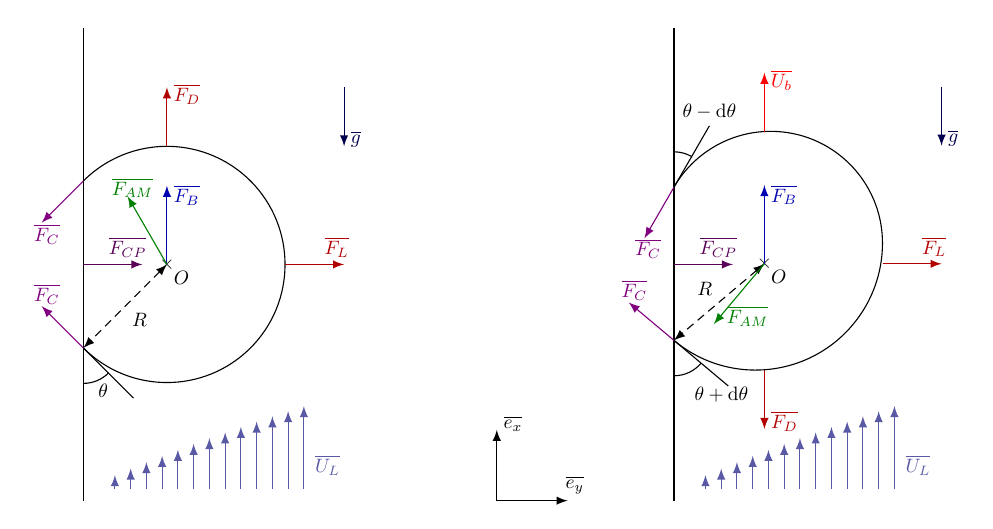
\begin{tikzpicture}[scale=3.0, every node/.style={scale=0.7}]


%%%Truncated sphere on a vertical wall

\coordinate (O1) at (0,0);
\coordinate (O2) at (0,2);

\draw (O1)--(O2);

\coordinate (Ob) at (0,1.0);

\tikzmath{\thet = 45; \thetrad= \thet * pi / 180; \ray=0.5; \rw=\ray * sin(\thetrad r);};


\coordinate (Oarc) at ($(Ob)-(0,{\ray * sin(\thetrad r)})$);
\draw (Oarc) arc({(-pi+\thetrad ) r}:{(pi-\thetrad ) r}:\ray);

%Upstream angle
\draw (Oarc) --++(-90+\thet:0.3);
\draw ($(Oarc)+(0,-0.15)$) arc(-90:-90+\thet:0.15) node[near end, below]{$\theta$};

%%Downstream angle
%\coordinate (Oarc2) at ($(Oarc) - (2*\rw,0)$);
%\draw (Oarc2) --++(180-\thet:0.3);
%\draw ($(Oarc2)+(-0.15,0)$) arc(180:180-\thet:0.15) node[near end, left]{$\alpha$};

%Center and radius

\coordinate (Cb) at ($(Ob)+({\ray*cos(\thetrad r)},0 )$);
\draw (Cb) node{$\times$} node[below right]{$O$};

\draw[densely dashed, <->, >=latex] (Cb) -- (Oarc) node[midway, below right]{$R$};


%%Forces

\draw[->, >=latex, violet!70!black] (Ob)--++(\ray/2,0) node[near end, above]{$\vect{F_{CP}}$};

\draw[->, >=latex, red!70!black!] ($(Cb)+(\ray,0)$)--++(\ray/2,0) node[very near end, above]{$\vect{F_{L}}$};
\draw[->, >=latex, red!70!black!] ($(Cb)+(0,\ray)$)--++(0,\ray/2) node[very near end, right]{$\vect{F_{D}}$};

\coordinate (Oarc2) at ($(Oarc)+(0,{2*\rw})$);
\draw[->, >=latex, violet] (Oarc)--++(90+\thet:\ray/2) node[very near end, above]{$\vect{F_{C}}$};
\draw[->, >=latex, violet] (Oarc2)--++(-90-\thet:\ray/2) node[very near end, below]{$\vect{F_{C}}$};

\draw[->, >=latex, blue!70!black] (Cb)--++(0,\ray/1.5) node[very near end, right]{$\vect{F_{B}}$};


\draw[->, >=latex, green!50!black!] (Cb)--++(90+\thet/1.5:\ray/1.5) node[very near end, above]{$\vect{F_{AM}}$};

%Gravity

\draw[->, >=latex, blue!30!black]  ($(Cb)+({1.5*\ray},{1.5*\ray})$)--++(0,-\ray/2) node[very near end, right]{$\vect{g}$};


%Flow arrows
\foreach \i in {2,...,14} 
{
\coordinate (Oloc) at ($(O1)+(\i/15,0.05)$);
\draw[->,>=latex, gray!70!blue] (Oloc)--++(0,{ln(1+0.03*\i)});
}
\draw[gray!70!blue] ($(Oloc)+(0.1,0.1)$) node{$\vect{U_{L}}$};

%Referential vectors
\coordinate (Ovect) at (1.75,0);
\draw[->, >=latex] (Ovect)--++(0.3,0) node[very near end, above right]{$\vect{e_{y}}$};
\draw[->, >=latex] (Ovect)--++(0,0.3) node[very near end, above right]{$\vect{e_{x}}$};




%Tilted bubble
\coordinate (Ob2) at (2.5,1.0);

\coordinate (O1) at (2.5,0);
\coordinate (O2) at (2.5,2);
\draw (O1)--(O2);

\tikzmath{\thet = 40; \thetrad= \thet * pi / 180;
\dthet=10; \dthetrad=\dthet*pi/180;
\thetadvrad=\thetrad - \dthetrad;
\thetrecrad=\thetrad + \dthetrad;
\thetadv=\thetadvrad*180/pi;
\thetrec=\thetrecrad*180/pi;
\ray=0.5; 
\rayadv=\ray *(1+cos(\thetrad r))/(1+ cos(\thetadvrad r);
\rayrec=\ray *(1+cos(\thetrad r))/(1+ cos(\thetrecrad r);};

\coordinate (Oarc) at ($(Ob2)-(0,{\ray * sin(\thetrad r)})$);


\draw (Oarc) arc({-pi+(\thetrecrad)) r}:{0 r}:\rayrec) arc ({0 r}:{pi-(\thetadvrad)) r}:\rayadv);

%Upstream angle
\draw (Oarc) --++(-90+\thetrecrad r:0.3) node[very near end, below]{$\theta + \dtheta$};
\draw ($(Oarc)+(0,-0.15)$) arc(-90:-90+\thetrecrad r:0.15) ;

%Downstream angle
\coordinate (Oarc2) at ($(Oarc) + (0,{\rayadv * sin(\thetadvrad r) + \rayrec * sin(\thetrecrad r)})$);
\draw (Oarc2) --++({90-(\thetadvrad r)}:0.3);
\coordinate (angadv) at ($(Oarc2) +({90-(\thetadvrad r)}:0.3)$);
\draw (angadv)  node[above]{$\theta - \dtheta $};
\draw ($(Oarc2)+(0,+0.15)$) arc(90:{90-(\thetadvrad r)}:0.15);



%Center and radius

\coordinate (Cb) at ($(Oarc2)+( {\ray * cos(\thetrad r)} , {-0.5 * (\rayadv * sin(\thetadvrad r) + \rayrec  * sin(\thetrecrad r) )})$);
\draw (Cb) node{$\times$} node[below right]{$O$};

\draw[densely dashed, <->, >=latex] (Cb) -- (Oarc) node[midway, above left]{$R$};


%Inclination angle

%\draw[densely dotted] (Cb) --++ (0.7,0);
%\draw[densely dotted] (Cb) --++ ({(1*\dthetrad r)}: 0.7 );
%\draw ($(Cb) + (0.3,0)$) arc(0: {(\dthetrad r)}:0.3)  node[midway, right]{$\dtheta$};
%
%



%%Forces

\draw[->, >=latex, violet!70!black] (Ob2)--++(\ray/2,0) node[near end, above]{$\vect{F_{CP}}$};

\draw[->, >=latex, red!70!black!] ($(Cb)+(\ray,0)$)--++(\ray/2,0) node[very near end, above]{$\vect{F_{L}}$};
\draw[->, >=latex, red!70!black!] ($(Cb)+(0,-\rayadv*0.95)$)--++(0,-\ray/2) node[very near end, right]{$\vect{F_{D}}$};
\draw[->, >=latex, red] ($(Cb)+(0,+\rayrec*1.04)$)--++(0,+\ray/2) node[very near end, right]{$\vect{U_{b}}$};


\draw[->, >=latex, violet] (Oarc)--++(90+\thetrec:\ray/2) node[very near end, above]{$\vect{F_{C}}$};
\draw[->, >=latex, violet] (Oarc2)--++(-90-\thetadv:\ray/2) node[very near end, below]{$\vect{F_{C}}$};

\draw[->, >=latex, blue!70!black] (Cb)--++(0,\ray/1.5) node[very near end, right]{$\vect{F_{B}}$};


\draw[->, >=latex, green!50!black!] (Cb)--++(90-\thet:-\ray/1.5) node[very near end, right]{$\vect{F_{AM}}$};

%Gravity

\draw[->, >=latex, blue!30!black]  ($(Cb)+({1.5*\ray},{1.5*\ray})$)--++(0,-\ray/2) node[very near end, right]{$\vect{g}$};



%Flow arrows
\foreach \i in {2,...,14} 
{
\coordinate (Oloc) at ($(O1)+(\i/15,0.05)$);
\draw[->,>=latex, gray!70!blue] (Oloc)--++(0,{ln(1+0.03*\i)});
}
\draw[gray!70!blue] ($(Oloc)+(0.1,0.1)$) node{$\vect{U_{L}}$};



\end{tikzpicture}

}

\includegraphics[width=0.6\linewidth]{img/bub_dyn/bub_bdf.pdf}
\caption{Sketch of the forces applied to the bubble facing an upward flow $\vect{U_{L}}$ and sliding at velocity $\vect{U_{b}}$}
\label{fig:bub_forces}
\end{figure}



Regarding the bubble shape, we consider a quasi-spherical bubble of radius $R$ with a circular contact area with the wall of radius $r_{w}$. 


\begin{remark*}{}
This assumption is mainly supported for high pressure boiling where bubble elongation and deformation is not observed \cite{kossolapov_experimental_2021}. At lower pressure, the bubble shape can somewhat deviate from a spherical shape especially before lift-off. It seems however reasonably quasi-spherical at early growth stages \cite{maity_effect_2000}. 
\end{remark*} 


The bubble has a static contact angle $\theta$ and is tilted under the influence of the flow by an inclination angle $\dtheta$ (half the total angle hysteresis). The resulting downstream and upstream contact angles are therefore $\theta_{d}=\theta-\dtheta$ and $\theta_{u}=\theta+\dtheta$. If the bubble has a shape close to a truncated sphere, we can approximate the bubble foot radius as:

\begin{equation}
r_{w} \approx R~ \sin{\frac{\theta_{u}+\theta_{d}}{2}}=R~ \sin{\theta}
\label{eq:rw}
\end{equation}

Some authors rather take $r_{w}\approx \dfrac{1}{2} R~\parth{\sin{\theta_{u}} + \sin{\theta_{d}} }=R~\sin{\theta}\cos{\dtheta}$, however this expression tends to zero when reaching $\dtheta \to 90\degree$ which is undesirable regarding the expression of forces such as Contact Pressure and Surface Tension.


We suppose $V_{b}\approx\frac{4}{3}\pi R^{3}$ for the bubble volume.





\subsection{Buoyancy and Contact Pressure Force}

Following the work of Thorncroft \etal \cite{thorncroft_bubble_2001} and Duhar \& Colin \cite{duhar_dynamics_2006}, the global force balance for a bubble growing on a wall can be written as:

\begin{equation}
\underbrace{ \frac{4}{3} \pi R^{3} \rho_{V} \vect{g}}_{\text{Bubble weight}} + \vect{F_{C}} - \underbrace{ \int_{S_{b}} \parth{P_{L} - \rho_{L}gz}\vect{n}\ \mathrm{d}S }_{\text{Outer liquid pressure}} - \underbrace{ \int_{S_{w}} P_{V} \vect{n}\ \mathrm{d}S }_{\text{Inner vapor pressure}} + \underbrace{ \int_{S_{b}} \tens{\tau_{L}}\cdot \vect{n} }_{\text{Viscous efforts}} = \vect{0}
\end{equation}
where $\vect{n}$ is the local normal unity vector, $S_{b}$ is the bubble surface facing the liquid, $S_{w}$ the wall-contact area and $\tens{\tau_{L}}$ the deviatoric stress tensor associated to viscous effects.

\npar

Re-writing the two pressure integrals versus the liquid pressure at the wall $P_{0}$ yields:

\begin{align}
\nonumber- \int_{S_{b}}\parth{P_{L} - \rho_{L}gz}\vect{n}\ \mathrm{d}S - \int_{S_{w}} P_{V}\vect{n}\ \mathrm{d}S =& - \int_{S_{b} + S_{w}} \parth{P_{0} - \rho_{L}gz}\vect{n}\ \mathrm{d}S + \int_{S_{w}} \parth{P_{0} - \rho_{L}gz - P_{V}}\vect{n}\ \mathrm{d}S \\
\nonumber & - \int_{S_{b}} \parth{P_{L}-P_{0}}\vect{n}\ \mathrm{d}S \\
\nonumber & = \int_{S_{b} + S_{w}} \rho_{L} g z \vect{n}\ \mathrm{d}S + \int_{S_{w}}\parth{P_{0} - P_{V}}\vect{n}\ \mathrm{d}S\\
& - \int_{S_{b}} \parth{P_{L} - P_{0}}\vect{n}\ \mathrm{d}S
\label{eq:buoy_cp_derivation}
\end{align}

Summing the first term on the RHS of Eq. \ref{eq:buoy_cp_derivation} with the bubble weight results in the buoyancy force:


\begin{equation}
\vect{F_{B}}= V_{b}\parth{\rho_{V}-\rho_{L}}\vect{g}=\frac{4}{3}\pi R^{3}\parth{\rho_{L}-\rho_{V}}g \ \vect{e_{x}}
\label{eq:force_buoyancy}
\end{equation}


The second term of Eq. \ref{eq:buoy_cp_derivation} is the so-called "contact pressure force" and can be expressed versus the difference of liquid and vapor pressure at the bubble top:

\begin{align}
\int_{S_{w}} \parth{P_{0} - P_{V}}\vect{n} \mathrm{d}S &= \parth{P_{0}-P_{V}}\pi r_{w}^{2}\vect{e_{y}}\\
&= \parth{P_{L} - P_{V} - \rho_{L}gh} \pi r_{w}^{2} \vect{e_{y}}
\end{align}
where $P_{L}$ is the liquid pressure at the bubble top and $h$ the bubble height.

\npar
Using Laplace's equation $\Delta P = 2\sigma / R_{c}$ and assuming that $\rho_{L}gh \ll \Delta P$ yields:

\begin{align}
\vect{F_{CP}}  \approx \frac{2\sigma}{R_{c}} \pi r_{w}^{2}\  \vect{e_{y}}
\approx \pi R \sigma\ 2\ \sin{\theta}^{2}\ \vect{e_{y}}
\label{eq:FCP}
\end{align}

Here, $R_{c}$ is the curvature radius of the bubble which is often assumed to be equal to $5R$ \cite{klausner_vapor_1993, sugrue_modified_2016, mazzocco_reassessed_2018} without other explanation than avoiding an overestimation of the contact pressure force. To avoid this arbitrary choice, following the hypothesis of a nearly spherical bubble shape gives $R_{c}=R$.


\subsection{Capillary Force}

The capillary force acts at the triple contact line at the bubble's foot and is an important adhesive force maintaining the bubble attached to the wall. Its derivation can be done by integration of the effort exerted over the triple contact line. Noting $\Phi$ the polar angle around the bubble foot, we have :


\begin{equation}
\vect{F_{C}} = 2 \int_{0}^{\pi} \sigma r_{w} \vect{\tau}\parth{\Phi} \mathrm{d}\Phi
\end{equation}
where $\vect{\tau}$ is the unit vector tangent to the interface and perpendicular to the contact line.

To compute the resulting components parallel and tangent to the wall, Klausner \etal \cite{klausner_vapor_1993} account for a contact angle difference between the upstream (receeding) contact angle $\theta_{u}$ and downstream (advancing) contact angle $\theta_{d}$. If the local contact angle is noted $\gamma$, then:

\begin{equation}
\vect{\tau}\parth{\Phi} = \cos{\gamma} \cos{\Phi} \vect{e_{x}} + \sin{\gamma} \vect{e_{y}}
\end{equation}

Then assuming to represent the evolution of the local contact angle $\gamma$ from $\theta_{u}$ to $\theta_{d}$ using a polynomial expression of degree 3:


\begin{equation}
\gamma\parth{\Phi} = \theta_{d} + \parth{\theta_{u} - \theta_{d}} \crocht{3\parth{\frac{\Phi}{ \pi}}^{2} - 2\parth{\frac{\Phi}{\pi}}^{3}},\ 0 \leq \Phi \leq \pi
\label{eq:forces_klausner_poly_deg3}
\end{equation}
which verifies symmetry conditions:

\begin{equation}
\gamma'\parth{0} = \theta_{d},\ \gamma\parth{\pi} = \theta_{u},\ \gamma'\parth{0}=\gamma'\parth{\pi}=0
\end{equation}

To obtain an analytic expression, Klausner \etal also consider a first order linear interpolation:

\begin{equation}
\gamma\parth{\Phi} \approx \theta_{d} + \parth{\theta_{u}-\theta_{d}}\frac{\Phi}{\pi}
\end{equation}

This yields:

\begin{equation}
\vect{F_{C}}=-2r_{w}\sigma \frac{\pi\parth{\theta_{u}-\theta_{d}}}{\pi^{2}-\parth{\theta_{u}-\theta_{d}}^{2}}\parth{\sin{\theta_{u}}+\sin{\theta_{d}} }\vect{e_{x}} - 2r_{w} \sigma \frac{\pi}{\theta_{u}-\theta_{d}}\parth{\cos{\theta_{d}}- \cos{\theta_{u}}}\vect{e_{y}}
\label{eq:forces_FC_klausner_deg1}
\end{equation}

By comparing the analytic expression of Eq. \ref{eq:forces_FC_klausner_deg1} with the values obtained by numerical integration of Eq.\ref{eq:forces_klausner_poly_deg3}, Klausner \etal introduce a correction factor of $1.25$ over the $x$ component, finally giving :

\begin{align}
\vect{F_{C}}&=-2.5r_{w}\sigma \frac{\pi\parth{\theta_{u}-\theta_{d}}}{\pi^{2}-\parth{\theta_{u}-\theta_{d}}^{2}}\parth{\sin{\theta_{u}}+\sin{\theta_{d}} }\vect{e_{x}} - 2r_{w} \sigma \frac{\pi}{\theta_{u}-\theta_{d}}\parth{\cos{\theta_{d}}- \cos{\theta_{u}}}\vect{e_{y}}\\
%
&=-\pi R \sigma \underbrace{\crocht{2.5~ \frac{r_{w}}{R} \frac{\dtheta}{\parth{\frac{\pi}{2}}^{2}-\dtheta^{2}}\sin{\theta}\cos{\dtheta}}}_{f_{C,x}} \vect{e_{x}} - \pi R \sigma \underbrace{\crocht{2\ \frac{r_{w}}{R} \sin{\theta} \frac{\sin{\dtheta}}{\dtheta}}}_{f_{C,y}} \vect{e_{y}}
\label{eq:forces_FC}
\end{align}

\begin{remark*}{}
We can see that $f_{C,x} \to 0$ and $f_{C,y} \to 2\dfrac{r_{w}}{R}\sin{\theta}$  when $\dtheta \to 0$. In that case, $\vect{F_{C}} = -\vect{F_{CP}}$.
\end{remark*}





\subsection{Drag and Lift Forces}
\label{subsec:drag_lift}


The external liquid flow over the bubble induces the well-known drag and lift forces, acting respectively in the flow direction and perpendicular to the flow. They are usually expressed using associated coefficients $C_{D}$ and $C_{L}$ defined by:
\begin{align}
\vect{F_{D}}=&\frac{1}{2}C_{D}\rho_{L}S_{p} \norm{ \vect{U_{L}}-\vect{U_{b}} } \parth{\vect{U_{L}}-\vect{U_{b}}} \\
\vect{F_{L}}=&\frac{1}{2}C_{L}\rho_{L}S_{p}\norm{\vect{U_{L}}-\vect{U_{b}}}^{2}\ \vect{e_{y}}
\end{align}
with $S_{p}=\pi R^{2}$ the projected area of the bubble in the direction of the flow.

\subsubsection{Drag Coefficient}

Derivations of analytic expressions for the drag coefficient in an infinite fluid medium exist for more than a century, starting with Hadamard-Rybzinski (1911) \cite{hadamard_mouvement_1911}:

\begin{equation}
C_{D} = \frac{16}{\Re_{b}},\ \text{if}\ \Re_{b}<1
\end{equation}
where $\Re_{b} = \frac{\bars{U_{rel}}D_{B}}{\nu_{L}}$ is the bubble Reynolds number and $U_{rel} = U_{L} - U_{b}$ the relative velocity between the bubble and the surrounding fluid.

For $\Re_{b} \gg 1$, Levich (1962) \cite{levich_physicochemical_1962} found for a potential flow:

\begin{equation}
C_{D} = \frac{48}{\Re_{b}}
\end{equation}


For intermediate values of $\Re_{b}$, traditional approaches rely on expressions of the drag force for a bubble in an infinite medium based on numerical correlations as proposed by Mei \& Klausner \cite{mei_unsteady_1992}, used in many different mechanistic approaches \cite{zeng_unified_1993-1, thorncroft_bubble_2001, chen_prediction_2012, sugrue_modified_2016, ren_development_2020}:

\begin{equation}
C_{D,U} = \frac{16}{\Re_{b}}\crocht{1 + \parth{\frac{8}{\Re_{b}}+ \frac{1}{2}\parth{1+\frac{3.315}{\sqrt{\Re_{b}}} }}^{-1} }
\label{eq:CD_mei}
\end{equation}


Results from DNS conducted by Legendre \etal \cite{legendre_lift_1998} proposed expressions of the drag and lift forces for a hemispherical bubble on a wall facing a viscous shear flow. Earlier, Legendre \& Magnaudet \cite{legendre_lift_1998} analytically derived coefficients to transpose drag and lift expressions for a particle to the case of a bubble. This was applied by Mazzocco \etal \cite{mazzocco_reassessed_2018} to the Drag for a solid particle near a wall in a shear flow proposed by Zeng \etal \cite{zeng_forces_2009}.

\npar

In this work, we propose to rely on the recent work of Shi \etal \cite{shi_drag_2021} who conducted DNS of a shear flow over a spherical bubble of constant radius close to a wall for bubble Reynolds number between $10^{-1}$ and $10^{3}$ and non-dimensional shear rates between -0.5 and 0.5. A sketch of the situation simulated by Shi \etal is depicted on Figure \ref{fig:shi_scheme}.

\begin{figure}[h!]
\centering
\includegraphics[width=0.55\linewidth]{img/bub_dyn/shi_scheme.pdf}
\caption{Physical situation considered by Shi \etal \cite{shi_drag_2021}.}
\label{fig:shi_scheme}
\end{figure}


They computed the resulting drag and lift coefficients for each simulations and proposed correlations fitting their numerical results. The total Drag coefficient is expressed as a correction of the Drag coefficient for a bubble in an unbounded uniform flow  $C_{D,U}$. The total drag is given by:

\begin{equation}
C_{D}=\parth{1+\Delta C_{D}}C_{D,U}
\end{equation}
where $\Delta C_{D}$ accounts for both the effect of the shear flow and the wall vicinity. 

\npar
To cover the whole range of bubble Reynolds numbers, correlations at low and high $\Re_{b}$ are smoothly connected using an exponential term.

\begin{equation}
\Delta C_{D}=\Delta C_{D,\Re_{b}=O\parth{1}}+\parth{1-e^{-0.07\Re_{b}}}\Delta C_{D,{\Re_{b}\gg 1}}
\label{eq:drag_corr_shi}
\end{equation}


Each of those corrections is computed depending on $\Re_{b}$,  the non-dimensional shear rate $\Sr = \dfrac{2 \gamma R}{\bars{U_{rel}} }$ where $\gamma = \dpartial{U_{L,x}}{y}$, the non dimensional wall distance $L_{R} = \dfrac{y}{R}$   ($L_{R}=1$ being a spherical bubble laying on a wall) and non-dimensional viscous (or Stokes) length $L_{u}=\dfrac{y}{\nu_{L}/\bars{U_{rel}}}$. 


\begin{align}
\nonumber \Delta C_{D,\Re_{b}=O\parth{1}} = & \frac{1+\mathrm{tanh}\parth{0.012\Re_{b}^{0.8}} + \mathrm{tanh}\parth{0.07\Re_{b}^{0.8}}^{2}}{1+0.16L_{u}\parth{L_{u}+4}}\\
& \times \left[ \left(\frac{3}{8}L_{R}^{-1} + \frac{3}{64}L_{R}^{-4}\right) \left(1- \frac{3}{8}L_{R}^{-1}-\frac{3}{64}L_{R}^{-4}\right)^{-1} - \frac{1}{16}\left(L_{R}^{-2}+\frac{3}{8}L_{R}^{-3}\right)\text{Sr} \right] \\
%
\nonumber\\
\Delta C_{D,{\Re_{b}\gg 1}} =& ~0.47L_{R}^{-4}+0.0055L_{R}^{-6}\Re_{b}^{3/4} 
+0.002 \bars{\mathrm{Sr}}^{1.9} \Re_{b} + 0.05 L_{R}^{-7/2} \mathrm{Sr} \Re_{b}^{1/3}
\end{align}


Figure \ref{fig:CD_shi} shows the evolution of the drag correction $\Delta C_{D}$ against the bubble Reynolds number for different dimensionless distances to the wall $L_{R}$ and two values of $\Sr$.  We can see that as the distance between the wall and the bubble increases the drag correction logically approaches zero and that increasing the shear rate $\Sr$ increases $\Delta C_{D}$ for higher values of $\Re_{b}$.

\npar

Shi \etal \cite{shi_drag_2021} conducted DNS for wall distances down to $L_{R}=1.5$. However, Scheiff \etal \cite{scheiff_experimental_2021} compared the values obtained for $L_{R}=1$  with measured drag coefficients of bubbles sliding on a wall and observed a good agreement, which legitimates the use of this new drag correlation by extending its application to the case of a bubble laying on a wall and using the uniform drag coefficient of Eq.~\ref{eq:CD_mei}.


\begin{figure}[h!]
\centering
\includegraphics[width=0.6\linewidth]{img/bub_dyn/forces/corr_drag.pdf}
\caption{Drag correction from Shi \etal \cite{shi_drag_2021}.}
\label{fig:CD_shi}
\end{figure}


\begin{remark*}{}
In PWR conditions, a static bubble of radius $0.01$\ mm on a wall with a bulk liquid velocity of $5$\ m/s leads to a non-dimensional shear rate $\Sr \approx 0.7$ with $\Re_{b} \approx 500$. In this case, the drag correction can reach 180\% compared to the unbounded uniform flow formulation.

\npar

This also yields a bubble Weber number $\We \approx 0.08$ and a Capillary number $\Ca \approx 0.0036$ which further supports the assumption of spherical bubble shape.
\end{remark*}


\subsubsection{Lift Coefficient}


In 1987, Auton \etal \cite{auton_lift_1987} analytically derived the lift force for an inviscid fluid in unstationnary motion in a weak velocity gradient and found $C_{L}=0.5$, with the lift force defined as:

\begin{equation}
\vect{F_{L}} = - \rho_{L} C_{L} V_{b} \parth{\vect{U_{L}} - \vect{U_{b}}} \wedge \vect{\omega} 
\end{equation} 
where $\vect{\omega}$ is the flow vorticity.

\npar
This result was enriched by Legendre \& Magnaudet (1998) \cite{legendre_lift_1998} who used numerical results to propose a dependency of $C_{L}$ on the bubble Reynolds number for a sphere in an infinite medium facing a weakly sheared flows as:

\begin{align}
C_{L} =&\parth{ {C_{L,\Re_{b} \sim 1}}^{2} + {C_{L,\Re_{b} \gg 1}}^{2} }^{1/2}\\
 =&\parth{ \crocht{\frac{6}{\pi^{2}} \frac{2.255 \parth{\Re_{b}\omega^{*}}^{-1/2}}{ \parth{1+0.2\dfrac{\Re_{b}}{\omega^{*}}}^{3/2} }}^{2} + \crocht{ \frac{1}{2} \frac{1+16\ {\Re_{b}}^{-1}}{1+29\ {\Re_{b}}^{-1}} }^{2} }^{1/2}
\end{align} 
where $\omega^{*} = \dfrac{2R\bars{\vect{\omega}}}{\bars{U_{rel}}}$ is the non-dimensional vorticity of the flow, equal to $\Sr$ here for the linear shear flow case.
%
%\begin{remark*}{}
%In the case of a steady linear shear flow near a wall, the vorticity is $\vect{\omega}=\overline{\nabla} \wedge \vect{U_{L}}=-\gamma\ \vect{e_{y}}$. In that case, the non-dimensional vorticity becomes the non-dimensional shear rate : $\omega^{*} = \dfrac{2R\gamma}{\bars{U_{rel}}} = \Sr$.
%\end{remark*}


\npar

Later, Mei \& Klausner (1994) \cite{mei_shear_1994} derived the lift force induced by the shear for a spherical bubble in an unbounded flow for low Reynolds numbers, based on the expression of Saffmann \cite{saffman_lift_1965}. By interpolating this result with the solution of Auton \cite{auton_lift_1987}, they obtained a formulation for a large range of $\Re_{b}$ :

\begin{equation}
C_{L} = 2.74 \sqrt{\Sr} \times \crocht{\Re_{b}^{-2} + \parth{0.24\sqrt{\Sr}}^{4}}^{1/4}
\label{eq:lift_mei}
\end{equation}

This expression is actually used in many mechanistic force balance \cite{klausner_vapor_1993, chen_prediction_2012, sugrue_modified_2016, ren_development_2020}.


\npar

In his force-balance approach, Mazzocco \etal \cite{mazzocco_reassessed_2018} used a constant lift coefficient by using the upper bound for the lift of a solid particle touching a wall in a Stokes flow, multiplied by $\dfrac{4}{9}$ to transpose this value to the bubble case as suggested by Legendre \& Magnaudet \cite{legendre_lift_1998}. This resulted in:

\begin{equation}
C_{L} = 2.61
\end{equation}


\npar

In accordance with the computation of the drag coefficient, our model will rely on the expression of the lift coefficient proposed by Shi \etal \cite{shi_drag_2021}. Their formulation includes extra parameters compared to the drag coefficient :
\begin{itemize}
\item The non-dimensional Saffman length $L_{\omega} = \dfrac{y}{\sqrt{\nu_{L} / \omega}}$ ;
\item The Stokes (or Oseen) length to Saffman length ratio $\varepsilon = \dfrac{\nu_{L} / \bars{U_{rel}}}{\sqrt{\nu_{L} / \omega}}$, which quantifies the origin of inertial effects being either shear ($\varepsilon >1$) or the relative slip of the bubble ($\varepsilon < 1$).

\end{itemize}  

The resulting formulation of $C_{L}$ corresponds to the superpositions of two contributions respectively associated to the uniform flow and the shear rate, both coupled with the wall presence. 

\begin{align}
C_{L}^{W} =C_{Lu}^{W} + C_{L\omega}^{W}
\label{eq:lift_shi}
\end{align}



The lift associated to the uniform flow near a wall is computed as follows:
\begin{align}
\nonumber C_{Lu}^{W} =&\  e^{-0.22\ \varepsilon^{0.8}L_{\omega}^{2.5}} \frac{ \crocht{1 + \tanh{0.012\ {\Re_{b}}^{0.8}} + \tanh{0.07\ {\Re_{b}}^{0.8}} }^{2} } {1+0.13\ L_{u} \parth{L_{u}+0.53} } \\
%
\nonumber			&\times  \parth{\frac{L_{R}}{3}}^{-2.0\ \tanh{0.01\Re_{b}}}  C_{Lu}^{\text{W-in}}\\
%
&+\parth{1-e^{-0.22\ {\Re_{b}}^{0.6}} } \crocht{ C_{Lu,\Re_{b}\to \infty}^{W} + 15\ \tanh{ 0.01\ \Re_{b} }{\Re_{b}}^{-1} L_{R}^{-4} }
%
\end{align}
Where:
\begin{align}
C_{Lu}^{\text{W-in}}=&\frac{1}{2}\left(1+\frac{1}{8}L_{R}^{-1}-\frac{33}{64}L_{R}^{-2}\right)\\
%
C_{Lu, \Re_{b} \to \infty}^{W} = & -\frac{3}{8}L_{R}^{-4}\left[1+\frac{1}{8}L_{R}^{-3}+\frac{1}{6}L_{R}^{-5}\right] + O\left(L_{R}^{-10}\right)
\end{align}


\npar

The lift associated to the vorticity near a wall is computed as follows:

\begin{align}
C_{L\omega}^{W} =& \crocht{ 1-\exp{ -\frac{11}{96}\pi^{2}\frac{L_{\omega}}{J_{L}(\varepsilon)} \parth{1+\frac{9}{8}L_{R}^{-1}-\frac{1271}{3520}L_{R}^{-2}} } }C_{L\omega, \Re_{b} \ll 1}^{U}\\
%
 & + \parth{1-e^{-0.3\ \Re_{b}} } \crocht{1+0.23\ L_{R}^{-7/2} \parth{1+13\ {\Re_{b}}^{-1/2}}} C_{L\omega, \Re_{b} \gg 1}^{U}
\end{align}

Where:

\begin{align}
J_{L}(\varepsilon)&=2.254 \parth{1+0.2\varepsilon^{-2}}^{-3/2} \\
%
C_{L\omega, \Re_{b} \ll 1}^{U} &= \frac{8}{\pi^{2}} \frac{\Sr}{\bars{\Sr}}\varepsilon J_{L}(\varepsilon)\\
%
C_{L\omega, \Re_{b} \gg 1}^{U}&= \frac{2}{3}\Sr \parth{ 1-0.07\bars{\Sr} }\frac{1+16\Re_{b}^{-1}}{1+29\Re_{b}^{-1}}
\end{align}


On Figure \ref{fig:lift_shi}, we plot the values of $C_{L}$ obtained by the formulation of Shi \etal different values of the non-dimensional wall distance $L_{R}$ (extending down to $L_{R}=1$) and non-dimensional shear rate $\Sr$.

\begin{figure}[h!]

\subfloat[Positive values of $\Sr$]{
\includegraphics[width=0.5\linewidth]{img/bub_dyn/forces/lift_shi_srpos.pdf}
}
\subfloat[Negative values of $\Sr$]{
\includegraphics[width=0.5\linewidth]{img/bub_dyn/forces/lift_shi_srneg.pdf}
}

\caption{$C_{L}$ computed using Shi \etal correlation.}
\label{fig:lift_shi}
\end{figure}

We can see that the magnitude of the lift coefficient globally increases with the wall distance when $\Sr >0$ and that negative lift values are easily reached when $\Sr <0$. This means that correlations for unbounded medium may overestimate the lift experienced by the bubble compared to the situation with a wall. 

The extension to the case $L_{R}=1$ may be more questionable compared to the drag since the bubble touching the wall will stop any flow in between, leading to inertial and shear regimes that would be significantly different due to the redirection of the liquid at the bubble's foot towards the bulk. In particular, we can see that the values reached for $L_{R}=1$ on Figure \ref{fig:lift_shi} are not following the general trend of simulated $L_{R}$ :

\begin{itemize}
\item Negative values of $C_{L}$ are reached with positive $\Sr$ at high $\Re_{b}$ while getting close to the wall seemed to tend to a value of $C_{L} \geq 0$ at high $\Re_{b}$ ;
\item Magnitude of $C_{L}$ with negative $\Sr$ are not coherent with the observed trend down to $L_{R}=1.5$.
\end{itemize}

This observation suggest that we should include the effect of the wall using the lift of Shi \etal by limiting its use to $L_{R}=1.5$ contrary to the drag which extension to $L_{R}=1.0$ was coherent and validated.

\npar

\begin{remark*}{}
In PWR conditions, taking $\Sr \approx 0.7$ with $\Re_{b} \approx 500$ for the static bubble on a wall leads to $C_{L}\approx 0.45$ both with Mei \& Klausner (Eq. \ref{eq:lift_mei}) and Shi \etal (Eq. \ref{eq:lift_shi}). For a bubble that would slide at 90\% of the local liquid velocity, this gives $\Sr \approx 7$ and $\Re_{b} \approx 50$ yielding $C_{L,Mei} \approx 4$ and $C_{L,Shi} \approx 2.8$.
\end{remark*}


\subsection{Inertia Force}
\label{subsec:AM}

The Inertia force originates from various effects (bubble growth, freestream and bubble acceleration, etc.) and includes both added mass and Tchen forces and is expressed as presented in Magnaudet \& Eames (2000) \cite{magnaudet_motion_2000}:

\begin{equation}
\vect{F_{I}} = \underbrace{ \rho_{L}V_{b}\parth{\dtime{\vect{U_{L}}}+\vecgrad{\vect{U_{L}} }\cdot \vect{U_{L}}} }_{\text{Liquid inertia or Tchen force}} + \underbrace{ \derive{}{t}\parth{\rho_{L}C_{AM}V_{b}\parth{\vect{U_{L}}-\vect{U_{b}}}} }_{\text{Added Mass force } \vect{F_{AM}}}
\label{eq:F_inertia}
\end{equation}

Since we consider a steady and quasi-parallel liquid flow, we respectively have:

\begin{equation}
\dpartial{\vect{U_{L}} }{t}=0\ \text{and}\ \vecgrad{\vect{U_{L}} } \cdot \vect{U_{L}}=0
\end{equation}

Thus only remains the added mass force to be expressed in the considered force balance. In the next subsections, we detail former approaches to tackle the added mass derivation and propose a more rigorous one to re-evaluate the added mass coefficients.


\subsubsection{Former Approaches}
\label{subsubsec:former_AM}

In previous mechanistic models, the derivation of the added mass force was conducted with different approaches. In particular, some authors chose to rely on the Rayleigh-Plesset Equation (RPE) for a growing hemispherical bubble in a quiescent flow to obtain the reaction force from the liquid, oriented perpendicularly to the wall:

\begin{equation}
\vect{F_{AM,RPE}}=- \rho_{L}\pi R^{2}\crocht{R\ddot{R}+\frac{3}{2}\dot{R}^{2}}\vect{e_{y}}
\end{equation}

Then, assuming a bubble inclination angle $\theta_{i}$, this force was projected along the $x$ axis to obtain an Added Mass force parallel to the wall that hinders departure. The inclination angle value is often empiricial and used for data fitting \cite{zeng_unified_1993-1, colombo_prediction_2015, mazzocco_reassessed_2018, ren_development_2020}.

\begin{equation}
\vect{F_{AM,RPE}}=- \rho_{L}\pi R^{2}\crocht{R\ddot{R}+\frac{3}{2}\dot{R}^{2}}\parth{\sin{\theta_{i}}\vect{e_{x}} + \cos{\theta_{i}}\vect{e_{y}}}
\label{eq:AM_RPE}
\end{equation}


This approach is questionable on different aspects. First, the RPE assumes a moving boundary in a quiescent unbounded liquid, which is physically far from the real situation of a bubble growing on a wall in a boiling flow. Moreover, the subsequent projection along the different directions regarding an unknown angle is hardly reasonable if $\theta_{i}$ is chosen arbitrarily. Values of $\theta_{i}$ selected by different authors are mentioned in Table \ref{tab:all_BdF}.

\npar

On the other hand, some authors \cite{klausner_vapor_1993, thorncroft_bubble_2001, guan_bubble_2015} considered two distinct contributions: 

\begin{itemize}

\item Hemispherical bubble growth in a stagnant liquid, leading to Eq.~\ref{eq:AM_RPE} including the inclination angle $\theta_{i}$ ;
\item Spherical bubble growth in a uniform unbounded and inviscid liquid flow, which yields a detaching Added Mass term  due to the interaction of bubble growth with the external flow: 
\begin{equation}
\vect{F_{AM,U}}= \frac{3}{2}\rho_{L}V_{b}\frac{\dot{R}}{R}U_{L} \vect{e_{x}} 
\label{eq:AM_bulk}
\end{equation} 

\end{itemize}

This last term is usually called a "bulk growth force". By including the effect of the liquid flow, this approach can be considered as closer to the reality. However, it relies on two separate derivations associated to different physical considerations.



\subsubsection{Proposed Approach}
\label{subsubsec:new_AM}

To tackle the added mass derivation in a proper way, we propose to follow the approach of Lamb \cite{lamb_hydrodynamics_1895} (also presented by Milne Thomson \cite{milne-thomson_theoretical_1938} or Van Winjgaarden \cite{wijngaarden_hydrodynamic_1976}). By solving the potential flow around a bubble and its image, we can obtain the total liquid kinetic energy $E_{L}$ that corresponds to a situation where a bubble is at a given distance from a wall (represented by the line normal to the line of centers of the bubbles). 

Then we can use Lagrange equation to compute the resulting forces along a given coordinate $q$:


\begin{align}
F_{AM,q}&=-\dpartial{}{t}\parth{\dpartial{E_{L}}{\dot{q}}}+\dpartial{E_{L}}{q}
\label{eq:lagrangian}
\end{align}


This method was also used by Duhar \cite{duhar_dynamics_2006} who developed an asymptotic expression of $E_{L}$ to compute the added mass coefficient when a growing bubble approaches the wall. Here, we express the liquid kinetic energy by relying on the work of Van Der Geld \cite{van_der_geld_dynamics_2009} who derived $E_{L}$ in the case of a full or truncated spherical bubble laying on a wall and facing an uniform flow parallel to the wall of velocity $U_{L}$ (Eq.~\ref{eq:EL_VdG}). If the bubble slides at a velocity $U_{b}=\dot{x}$, it sees a liquid velocity $U_{rel}=U_{L}-\dot{x}$.

\begin{align}
E_{L}=\frac{\rho_{L}V_{b}}{2}\parth{\alpha \dot{y}^{2} +\trb\dot{R}^{2}+\psi \dot{R}\dot{y} +\alpha_{2} \parth{U_{L}-\dot{x}}^{2} }
\label{eq:EL_VdG}
\end{align}
where $(x,y)$ are the coordinates of the bubble's center and $\alpha$, $\trb$, $\psi$, $\alpha_{2}$ are polynomials of $R/y = 1/L_{R}$ derived by Van Der Geld for $1<R/y<2$ \ie $0.5<L_{R}<1$, corresponding to contact angles $0\degree < \theta < 60\degree$.

\npar
For each polynomial expression ($\alpha$ is used as an example), we note $n$ its degree and write:

\begin{equation}
\alpha = \sum_{k=0}^{n}\alpha_{k}\parth{\frac{R}{y} }^{k}\ \text{and}\ \tilde{\alpha}= \sum_{k=0}^{n}k\ \alpha_{k}\parth{\frac{R}{y} }^{k}
\end{equation}

This allows to express the following derivatives:

\begin{equation}
\dpartial{\alpha}{y} = -\frac{1}{y} \tilde{\alpha}\ \text{and}\ \dpartial{\alpha}{t} = \parth{\frac{\dot{R}}{R} - \frac{\dot{y}}{y}} \tilde{\alpha}
\end{equation}


Noticing that the derivatives of the polynomials along $x$ will be 0 and injecting $E_{L}$ in Eq.~\ref{eq:lagrangian} allows to express the added mass force in $x$ and $y$ directions. If we express it using geometrical ratios $\dfrac{R}{y}=\dfrac{1}{F_{1}}$, $\dfrac{\dot{y}}{\dot{R}}=F_{2}$ and $\dfrac{\ddot{y}}{\ddot{R}}=F_{3}$, we can obtain:

\begin{align}
F_{AM,x} = \rho_{L}V_{b} \crocht{ \parth{ 3\alpha_{2} +\parth{1-\frac{F_{2}}{F_{1}}}\tilde{\alpha_{2}} } \frac{\dot{R}}{R}U_{rel} - \alpha_{2} \dtime{U_{b}} }
\end{align}

\begin{align}
\nonumber F_{AM,y} = - \rho_{L} V_{b} & \left[ \parth{ 3 F_{2}\alpha + \frac{3}{2}\psi + \parth{1- \frac{F_{2}}{F_{1}}}F_{2} \tilde{\alpha} + \parth{1- \frac{F_{2}}{F_{1}}}\frac{\tilde{\psi}}{2}  + \frac{F_{2}}{F_{1}}\frac{\tilde{\alpha}}{2} + \frac{1}{F_{1}} \frac{\tilde{\trb}}{2} + \frac{F_{2}}{F_{1}} \frac{\tilde{\psi}}{2}}\frac{\dot{R}^{2}}{R} \right.\\
& \left.  + \parth{F_{3}\alpha + \frac{\psi}{2}}\ddot{R} + \frac{1}{F_{1}}\frac{\tilde{\alpha_{2}}}{2} \frac{U_{rel}^{2}}{R}  \right] 
\end{align}


In the case of a truncated sphere, $F_{1} = \dfrac{y}{R} = \cos{\theta}=L_{R}$. If we suppose that the bubble keeps a nearly constant contact angle during its lifetime, we can further write $F_{1}=F_{2}=F_{3}=\cos{\theta}=L_{R}$, which simplifies the forces in:


\begin{align}
F_{AM,x} = \rho_{L}V_{b} \crocht{ 3\alpha_{2} \frac{\dot{R}}{R}U_{rel} - \underbrace{\alpha_{2}}_{C_{AM,x}} \dtime{U_{b}} }
\label{eq:FAMx}
\end{align}


\begin{align}
F_{AM,y} = \rho_{L} V_{b} & \left[  -\parth{ 3 \underbrace{\parth{L_{R}\alpha + \frac{\psi}{2} } }_{C_{AM,y1}} + \underbrace {\frac{\tilde{\alpha}}{2} + \frac{1}{L_{R}} \frac{\tilde{\trb}}{2} + \frac{\tilde{\psi}}{2}}_{C_{AM,y2}} } \frac{\dot{R}^{2}}{R} \right. \\
%
& \left. - \underbrace{ \parth{L_{R}\alpha + \frac{\psi}{2}} }_{C_{AM,y1}} \ddot{R} + \underbrace{ \frac{-1}{L_{R}}\frac{\tilde{\alpha_{2}}}{2} }_{C_{AM,y3}} \frac{U_{rel}^{2}}{R}  \right] 
\label{eq:FAMy}
\end{align}


On Figure \ref{fig:AM_coeff}, we plot the values of the added mass coefficients against the values of $L_{R}$. 

\begin{figure}[h!]
\centering
\includegraphics[width=0.65\linewidth]{img/bub_dyn/forces/CAM_plot.pdf}
\caption{Values of the computed added mass coefficients in Eq. \ref{eq:FAMx} and \ref{eq:FAMy}. }
\label{fig:AM_coeff}
\end{figure}

For the case of a spherical bubble laying on a wall ($L_{R}=1$), we finally have:



\begin{align}
F_{AM,x}=\rho_{L}V_{b}\crocht{3C_{AM,x}\frac{\dot{R}}{R}U_{rel} - C_{AM,x}\dtime{U_{b}}}
\label{eq:AMx}
\end{align}
with $C_{AM,x} \approx 0.636$.


\begin{align}
F_{AM,y}=\rho_{L}V_{b}\crocht{-\parth{3 C_{AM,y1} + C_{AM,y2}}\frac{\dot{R}^{2}}{R}-C_{AM,y1}\ddot{R} + C_{AM,y3}\frac{U_{rel}^{2}}{R}}
\label{eq:AMy}
\end{align}
with $C_{AM,y1} \approx 0.27$, $C_{AM,y2}\approx 0.326$ and $C_{AM,y3}\approx 8.77\times  10^{-3}$.


\npar

Parallel to the wall, the coupled term $\frac{\dot{R}}{R}U_{rel}$ in Eq.~\ref{eq:AMx} promotes detachment and sliding of the bubble if $U_{rel}>0$ \eg if the bubble is attached to its nucleation site. This contradicts the aforementioned approach where solely projecting the RPE on both axes lead to an Added-Mass term related to bubble growth that only hinders the departure by sliding. Moreover, Eq.~\ref{eq:AMy} exhibits a term induced by the relative velocity that acts as a lift force, which seems to rarely appear in other approaches.

\begin{remark*}{}
The derived values of the added mass coefficients are only valid for $0.5 < L_{R} < 1$ as previously mentioned. When the bubble leaves the wall, added mass calculations of Duhar \cite{duhar_croissance_2003} would be more appropriate.
\end{remark*}



\npar
Those theoretical results highlight the importance of conducting a rigorous approach when possible to deriving those transient aspects of the force balance. Otherwise, some terms may be missing and lead to contradictory physical conclusions. 

In the spirit of avoiding to introduce extra empirical terms, we keep the Added Mass force as presented in Eq.~\ref{eq:AMx} and \ref{eq:AMy} and consider no projection along the inclination angle.



\subsection{Force Balance Summary}\label{subsec:BdF}


Writing Newton's second law, we have the total force balance over the bubble in both directions:

\begin{align}
\nonumber \rho_{V} \dtime{V_{b}U_{b,x}} = & -\pi R \sigma f_{C,x}\parth{\theta, \dtheta} + V_{b}\parth{\rho_{L}-\rho_{V}}g + \frac{1}{2}C_{D}\rho_{L}\pi R^{2} \bars{U_{L}-U_{b}}\parth{U_{L}-U_{b}}\\
%
& + \rho_{L}V_{b}\crocht{3C_{AM,x}\frac{\dot{R}}{R}\parth{U_{L}-U_{b}} - C_{AM,x} \dtime{U_{b}}}
\label{eq:bdf_x}
\end{align}

\begin{align}
\nonumber \rho_{V} \dtime{V_{b}U_{b,y}} = & -\pi R \sigma f_{C,y}\parth{\theta, \dtheta} + 2\pi R \sigma \sin{\theta}^{2} + \frac{1}{2}C_{L}\rho_{L}\pi R^{2} \parth{U_{L}-U_{b}}^{2}\\
%
& + \rho_{L}V_{b}\crocht{-\parth{3 C_{AM,y1} + C_{AM,y2}}\frac{\dot{R}^{2}}{R}-C_{AM,y1}\ddot{R} + C_{AM,y3}\frac{\parth{U_{L}-U_{b}}^{2}}{R}}
\label{eq:bdf_y}
\end{align}

Those force balances will respectively be used later to study the departure by sliding (along $x$) and the lift-off from the wall (along $y$).

\npar

On Table \ref{tab:all_BdF}, we sum up some of the mentioned mechanistc approaches and their models along with the proposed force balance.



\begin{table}[h!]



\scriptsize
\centering

\noindent\makebox[\textwidth]{
\renewcommand{\arraystretch}{2.0}


\begin{tabular}{p{2mm} p{6mm}|p{50mm}|p{50mm}|p{50mm}}

 & & Klausner (1993) \cite{klausner_vapor_1993} & Thorncroft (2001) \cite{thorncroft_bubble_2001} & Sugrue (2016) \cite{sugrue_modified_2016} \\
\hline

\multirow{6}*{\rotatebox{90}{Forces}} &  $\vect{F_{B}}$ & $\frac{4}{3}\pi R^{3} \parth{\rho_{L}-\rho_{V}}\vect{g}$ & $\frac{4}{3}\pi R^{3}\parth{\rho_{L}-\rho_{V}}\vect{g}$ & $\frac{4}{3}\pi R^{3}\parth{\rho_{L}-\rho_{V}}\vect{g}$ \\

& $\vect{F_{C}}$ & Eq. \ref{eq:forces_FC}, $r_{w}=0.045$ mm & Eq. \ref{eq:forces_FC}, $r_{w}=R~\sin{\theta_{d}}$ & Eq. \ref{eq:forces_FC}, $r_{w}=0.025R$ \\

& $\vect{F_{CP}}$ &  Eq.~\ref{eq:FCP}, $R_{c}=5R$ &  Neglected &  Eq.~\ref{eq:FCP}, $R_{c}=5R$  \\

& \multirow{2}*{$\vect{F_{D}}$} & $C_{D}=\frac{16}{\Re_{b}} \left[ 1+\frac{3}{2} \left( \parth{\frac{12}{\Re_{b}}}^{n}\right. \right.$\newline$ \left. \left. \quad \quad + 0.796^{n} \right) ^{1/n} \right]$, $n=0.65$ & $C_{D} = \frac{16}{\Re_{b}} \left[ 1 + \left(\frac{8}{\Re_{b}} \right. \right.$\newline$\left. \left. \quad  \quad + \frac{1}{2}\parth{1+\frac{3.315}{\sqrt{\Re_{b}}} } \right)^{-1} \right]$ & $C_{D}=\frac{16}{\Re_{b}} \left[ 1+\frac{3}{2} \left( \parth{\frac{12}{\Re_{b}}}^{n}\right. \right.$\newline$ \left. \left. \quad \quad + 0.796^{n} \right) ^{1/n} \right]$, $n=0.65$ \\

& \multirow{2}*{$\vect{F_{L}}$} & $C_{L}=2.74\sqrt{\Sr}$\newline$\times\crocht{\Re_{b}^{-2} + \parth{0.24\sqrt{\Sr}}^{4} }^{\frac{1}{4}}$ & $C_{L}=0.71\sqrt{\Sr}$\newline$\times\crocht{\parth{\frac{1.15\mathrm{J}(\varepsilon)}{\sqrt{\Re_{b}}}}^{2} + \parth{\frac{3\sqrt{2\Sr}}{8}}^{2} }^{\frac{1}{2}}$ & $C_{L}=2.74\sqrt{\Sr}$\newline$\times\crocht{\Re_{b}^{-2} + \parth{0.24\sqrt{\Sr}}^{4} }^{\frac{1}{4}}$   \\

& \multirow{2}*{$\vect{F_{AM}}$} & {$\frac{3}{2}\rho_{L}V_{b}\frac{\dot{R}}{R}U_{L} \vect{e_{x}}$ {$-\rho_{L}\pi R^{2}\parth{\frac{3}{2}\dot{R}^{2} + R\ddot{R}}$\newline$\times \parth{\cos{\theta_{i}}\vect{e_{y}} + \sin{\theta_{i}}\vect{e_{x}}}$, $\theta_{i}=10\degree$ }} & {$2\pi \rho_{L}R^{2}\dot{R}U_{L}\vect{e_{x}}$} {$-\rho_{L}\pi R^{2}\parth{\frac{3}{2}\dot{R}^{2} + R\ddot{R}}$\newline$\times \parth{\cos{\theta_{i}}\vect{e_{y}} + \sin{\theta_{i}}\vect{e_{x}}}$, $\theta_{i}=45\degree$ } & {{$-\rho_{L}\pi R^{2}\parth{\frac{3}{2}\dot{R}^{2} + R\ddot{R}}$\newline$\times \parth{\cos{\theta_{i}}\vect{e_{y}} + \sin{\theta_{i}}\vect{e_{x}}}$, $\theta_{i}=10\degree$ }} \\
\hline
\end{tabular}
}

\npar

\noindent\makebox[\textwidth]{
\renewcommand{\arraystretch}{2.0}

\begin{tabular}{p{2mm} p{6mm}|p{50mm}|p{50mm}|p{50mm}}
 & & Mazzocco (2018) \cite{mazzocco_reassessed_2018} & Ren (2020) \cite{ren_development_2020} & Present model \\
\hline

\multirow{6}*{\rotatebox{90}{Forces}} &  $\vect{F_{B}}$ & $\frac{4}{3}\pi R^{3} \parth{\rho_{L}-\rho_{V}}\vect{g}$ & $\frac{4}{3}\pi R^{3} \parth{\rho_{L}-\rho_{V}}\vect{g}$ & $\frac{4}{3}\pi R^{3} \parth{\rho_{L}-\rho_{V}}\vect{g}$ \\

& $\vect{F_{C}}$ & Eq. \ref{eq:forces_FC}, $r_{w}=R/15$ & Eq. \ref{eq:forces_FC}, $r_{w}=0.2R$& Eq. \ref{eq:forces_FC}, $r_{w}=R\ \sin{\theta}$ \\

& $\vect{F_{CP}}$ & Eq.~\ref{eq:FCP}, $R_{c}=5R$ &  Eq.~\ref{eq:FCP}, $R_{c}=5R$ &  Eq.~\ref{eq:FCP}, $R_{c}=R$   \\

& \multirow{2}*{$\vect{F_{D}}$} & \multirow{2}*{$C_{D}=1.13\frac{24}{\Re_{b}}\parth{1+0.104\Re_{b}^{0.753}}$} & $C_{D}=\frac{16}{\Re_{b}} \left[ 1+\frac{3}{2} \left( \parth{\frac{12}{\Re_{b}}}^{n}\right. \right.$\newline$ \left. \left. \quad \quad + 0.796^{n} \right) ^{1/n} \right]$, $n=0.65$ & $C_{D}=C_{D,U}\parth{1+\Delta C_{D}}$ \newline $C_{D,U}$ by Eq. \ref{eq:CD_mei}, $\Delta C_{D}$ by Eq. \ref{eq:drag_corr_shi} \\

& \multirow{2}*{$\vect{F_{L}}$} & \multirow{2}*{$C_{L}=2.61$} & $C_{L}=2.74\sqrt{\Sr}$\newline$\times\crocht{\Re_{b}^{-2} + \parth{0.24\sqrt{\Sr}}^{4} }^{\frac{1}{4}}$ & \multirow{2}*{$C_{L}$ by Shi \etal \cite{shi_drag_2021}}   \\

& \multirow{2}*{$\vect{F_{AM}}$} & {$-\frac{1}{4}\pi \rho_{L} K^{4}\parth{\cos{\theta_{i}}\vect{e_{y}} + \sin{\theta_{i}}\vect{e_{x}}}$, $\sin{\theta_{i}}=0.2$, $\cos{\theta_{i}}=1$} & {$-\rho_{L}\pi R^{2}\parth{\frac{3}{2}\dot{R}^{2} + R\ddot{R}}$\newline$\times \parth{\cos{\theta_{i}}\vect{e_{y}} + \sin{\theta_{i}}\vect{e_{x}}}$, $\theta_{i}=15\degree$ } & {$\frac{F_{AM,x}}{\rho_{L}V_{b}}=C_{AM,x}\crocht{3\frac{\dot{R}}{R}U_{rel} - \dtime{U_{b}}}$, $C_{AM,x}=0.636$, $F_{AM,y}$ by Eq. \ref{eq:AMy}.} \\
\hline
\end{tabular}

}


\caption{Summary of different force-balance mechanistic approaches.}
\label{tab:all_BdF}
\end{table}


\subsection{Liquid Velocity}\label{subsec:liq_vel}

To compute the liquid velocity and shear rate at bubble center height, we use the wall law of Reichardt \cite{reichardt_vollstandige_1951}, which describes the velocity profile from the viscous sublayer to the logarithmic region in a single-phase flow.

\begin{align}
U_{L}^{+} =& \frac{1}{\kappa}\ln{1+\kappa y^{+}} + c \parth{1-e^{-y^{+}/\chi} + \frac{y^{+}}{\chi}e^{-y^{+}/3} }\\
%
\nonumber U_{L}=&U_{L}^{+}U_{\tau}
\end{align}
with $\kappa = 0.41$, $\chi = 11$ and $c=7.8$.

\begin{align}
\dpartial{U_{L}^{+}}{y^{+}} =& \frac{1}{1+\kappa y^{+}}+\frac{c}{\chi}\parth{e^{-y^{+}/\chi} + \parth{1-\frac{y^{+}}{3}}e^{-y^{+}/3}}\\
%
\nonumber \dpartial{U_{L}}{y} =& \gamma = \frac{U_{\tau}^{2}}{\nu_{L}} \dpartial{U_{L}^{+}}{y^{+}}
\end{align}

The friction velocity is computed using Mac Adams correlation \cite{mcadams_heat_1954}.

\begin{align}
U_{\tau} =& \sqrt{\frac{\tau_{w}}{\nu_{L}}}
\label{eq:utau_mcadams}\\
\tau_{w} =& 0.018~ \Re_{D_{h}}^{-0.182}~ \frac{G_{L}^{2}}{\rho_{L}}
\end{align}

\newpage


\section{Bubble Growth}
\label{sec:bub_growth}

\subsection{Introduction}

In order to properly represent the bubble dynamics, it is mandatory to model the evolution of the bubble radius over time \ie the bubble growth law. Since the bubble radius $R$ and its derivatives $\dot{R}$ and $\ddot{R}$ appear in the force balance (notably in the expression of the added mass force \ref{eq:FAMy}), failing to predict the evolution of the bubble with time will definitely result in a force unbalance.

\npar
The problem of the bubble growth during its lifetime on the wall, including the sliding phase, is still an open question that aims to cover various types of heat transfer mechanisms. First, two growth regimes exist for a boiling bubble:

\begin{itemize}
\item Inertial growth, which occurs at the beginning of nucleation for low temperature difference between liquid and vapor. The evolution of the bubble size can be solved by the mass and momentum balances, through the solution of Rayleigh (1917) \cite{rayleigh_viii_1917}. The form of the bubble growth is usually $R\parth{t} = A\times t$ (Mikic \& Rohsenow, \cite{mikic_bubble_1970}).

\item Heat diffusion growth happening post the inertial phase. This type of bubble growth has been widely studied by different authors \cite{plesset_growth_1954, scriven_dynamics_1959, zuber_dynamics_1961, mikic_bubble_1970} and is usually of the form $R\parth{t} = B\sqrt{t}$, derivable using the energy balance around the bubble.
\end{itemize}


Those two regimes can be compared using the non-dimensional time $t^{+}$ defined as:

\begin{align}
t^{+} = \frac{A^{2}}{B^{2}}t
\end{align}
where
\begin{equation}
A=\sqrt{b \frac{h_{LV}\rho_{V} \Delta T_{w} }{\rho_{L}T_{sat}} } \ \text{and}\ B=\sqrt{\frac{12}{\pi}\eta_{L}}\Ja
\end{equation}
with $b=\dfrac{2}{3}$ for a bubble in an infinite liquid medium and $b=\dfrac{\pi}{7}$ for a spherical bubble laying on a wall.

\npar

So that when $t^{+} \ll 1$, $R\parth{t} = At$ (inertial growth) and when $t^{+} \gg 1$, $R\parth{t}=B\sqrt{t}$ (heat diffusion growth). A general solution asymptotically covering the two regimes has been derived by Mikic \& Rohsenhow:

\begin{equation}
R^{+} = \frac{2}{3}\crocht{\parth{t^{+}+1}^{3/2}+{t^{+}}^{3/2}-1},\ R^{+}=\frac{R}{B^{2}/A},\ t^{+}=\frac{t}{B^{2}/A^{2}}
\end{equation}


In most cases associated to wall nucleation and boiling flows, experimental observations showed that bubbles' lifetime is long enough to be mostly of heat conduction nature \cite{kossolapov_experimental_2021, maity_effect_2000, zhou_experimental_2020}.

\begin{remark*}{}
Estimating the time $t$ at which the diffusive growth radius equals the inertia growth radius yields:
\begin{itemize}
\item $t\approx 0.39\ \mu$s for water at 1\ bar and $\Delta T_{w}=15$\ K
\item $t\approx 1.6\times 10^{-4}\ \mu$s for water at 150\ bar and $\Delta T_{w}=5$\ K
\end{itemize}
which insists on the validity of the nearly pure diffusive growth hypothesis.
\end{remark*}

\subsection{Heat Diffusion in Uniformly Superheated Liquid}

The analytic derivation of a bubble growth law in a pure heat diffusion regime has been tackled by various authors, mostly for the case of a bubble in a uniformly superheated and quiescent liquid. An reference solution is the work of Plesset \& Zwick (1954) \cite{plesset_growth_1954} who found an asymptotic solution for high values of $\Ja$:

\begin{equation}
R\parth{t} = \frac{2\sqrt{3}}{\sqrt{\pi}}\Ja\sqrt{\eta_{L}t}
\label{eq:growth_plesset}
\end{equation}

This result was generalized by Scriven (1959) \cite{scriven_dynamics_1959} who derived whatever the value of $\Ja$:

\begin{equation}
R\parth{t} = 2 \mathcal{F}\parth{\Ja}\Ja\sqrt{\eta_{L}t}
\label{eq:growth_scriven}
\end{equation} 
where $\mathcal{F}$ is implicitly defined by assuming $\dfrac{\rho_{L}}{\rho_{V}} \gg 1$:

\begin{equation}
\mathcal{F}\parth{\Ja}=\frac{F}{2\Ja^{2}},\ \text{and}\ \Ja = F\exp{\frac{3}{2}F} \int_{1}^{\infty}\frac{1}{x^{2}}\exp{-\frac{F}{x}-\frac{F}{2}x^{2}}\mathrm{d}x
\end{equation}
which falls back to $\mathcal{F}\parth{\Ja} \to \dfrac{\sqrt{3}}{\sqrt{\pi}}$ when $\Ja \gg 1$.

\npar
The general formulation of $\mathcal{F}$ has been verified by Legendre \etal \cite{legendre_thermal_1998} with Direct Numerical Simulation of spherical bubble growth in a quiescent superheated liquid.

\npar

Usually, most authors are accepting $R\parth{t} = K \Ja_{w} \sqrt{\eta_{L}t}$ for the bubble growth. With $K$ usually expressed as $K=\dfrac{2b}{\sqrt{\pi}}$ with $b$ being used as an adjustable constant depending on the flow conditions, the fluid and the heater properties, or derived analytically as presented before ($b=\sqrt{3}$ \cite{plesset_growth_1954}, $b=\dfrac{\pi}{2}$ \cite{forster_growth_1954}, $1 \leq b \leq \sqrt{3}$ \cite{zuber_dynamics_1961}, $b=1.56$ \cite{yun_prediction_2012}, $b=0.24$ \cite{yoo_development_2018}, etc.).

\npar

When the bubble presents a relative velocity with the ambient liquid, the disturbance of the thermal boundary layer around the liquid-vapor interface will impact its growth. This phenomenon has been numerically studied by Legendre \etal \cite{legendre_thermal_1998} who found that the ratio between the growth rate $\dot{R}$ and the relative velocity $U_{rel}$ was controlling the growth regime as follows:

\begin{itemize}
\item If $\dfrac{\dot{R}}{U_{rel}}\gg 1$, the regime is close to the static heat diffusion and correspond to the Scriven formulation (Eq. \ref{eq:growth_scriven}) ;

\item If $\dfrac{\dot{R}}{U_{rel}}\ll 1$, the relative velocity impacts the thermal boundary layer formation and leads to a growth matching the solution of Ruckenstein (1964) \cite{ruckenstein_mass_1964} where the Nusselt number at the liquid-vapor interface is:
\begin{equation}
\Nu = 2\sqrt{\frac{\Pe\parth{t}}{\pi}},\ \Pe\parth{t} = \Pr_{L}\times \Re_{b}\parth{t}
\end{equation}
In this case, the bubble growth is accelerated and $R \propto t^{2/3}$. 
\end{itemize}


\subsection{Microlayer Evaporation}
\label{subsec:microlayer}

In addition to the traditional heat diffusion from superheated liquid to the bubble through the liquid-vapor interface, bubble growth can also be enhanced by the evaporation of a so-called "microlayer". This term denotes a very thin layer of liquid (typically $\sim \mu$m \cite{kossolapov_experimental_2021}) which is trapped between the heated wall and the bubble base, as shown on Figure \ref{fig:ML_Urbano}. The existence of this microlayer has now been supported by both experimental visualizations \cite{kossolapov_experimental_2021, koffman_experimental_1983, chen_detailed_2017, chen_measurement_2020} and numerical investigations \cite{urbano_direct_2018, guion_simulations_2018, bures_modelling_2021}.

\begin{figure}[h!]
\centering
\includegraphics[width=0.7\linewidth]{img/growth/ML_urbano.PNG}
\caption{Microlayer appearing beneath the bubble in DNS conducted by and adapted from Urbano \etal \cite{urbano_direct_2018}.}
\label{fig:ML_Urbano}
\end{figure}


Parallel to the heat diffusion approach, some authors computed the bubble growth by considering a pure microlayer evaporation regime. A well-known model of this type has been derived by Cooper \& Lloyd in 1969 \cite{cooper_microlayer_1969} and considers the wall thermal properties so that:

\begin{align} 
R\parth{t} =& 2.5 \dfrac{\Ja}{\sqrt{\Pr_{L}}}\sqrt{\eta_{L}t}\ \text{if}\ \lambda_{w} \gg \lambda_{L} \\
%
R\parth{t} =& \dfrac{2}{\sqrt{\pi}} \sqrt{\dfrac{\lambda_{w}\rho_{w}c_{p,w}}{\lambda_{L}\rho_{L}c_{p,L}}}\ \text{if}\ \lambda_{w} \ll \lambda_{L}
\end{align}

\begin{remark*}{}
The parameter $ \sqrt{\dfrac{\lambda_{w}\rho_{w}c_{p,w}}{\lambda_{L}\rho_{L}c_{p,L}}}$ that accounts for the wall properties is the same used in the correlation of \"Unal for the maximum bubble diameter (Eq. \ref{eq:dlo_unal}).
\end{remark*}

The microlayer is also often taken into account for HFP modeling by enhancing the boiling heat flux through a computation of the microlayer volume \cite{kommajosyula_development_2020, demarly_new_2020}. 

\npar

However, the presence of a liquid microlayer beneath the nucleated bubble is not assured for every boiling conditions. Indeed, experimental observations recently realized by Kossolapov \cite{kossolapov_experimental_2021} showed that the microlayer only existed for pressures below 3 bars when using water as working fluid. Moreover, Direct Numerical Simulations of Urbano \etal \cite{urbano_direct_2018} where a full coupling between mass, momentum and energy balance was achieved managed to detect wether if the bubble grows in a contact-line regime or if a microlayer appears. They proposed a criterion based on the capillary and Jakob numbers determining the formation of a microlayer, further validated by extra Direct Numerical Simulations from B\'ures \& Sato \cite{bures_modelling_2021}:

\begin{equation}
\frac{\Ja \Ca}{\parth{\theta-\theta_{0}}^{3}} > \frac{1}{A^{3}},\ \theta_{0}=5\degree,\ A=313
\end{equation}

\begin{remark*}{}
Computing the capillary number using $\dot{R}=\dfrac{K\Ja}{2}\sqrt{\dfrac{\eta_{L}}{t}}$ as the interface velocity, we use Urbano \etal criterion to compute the time $t_{max}$ after which the microlayer would cease to exist. Applying this to PWR conditions ($K=1$, $\Delta T_{w}=5K$) yields $t_{max}<10^{-11}$s for $6\degree \leq \theta \leq 90\degree$, meaning that there is no time during the bubble growth during which a microlayer could grow. This agrees with the observation that increasing pressure would lead to microlayer disappearance.
\end{remark*}

We will not further detail the study of the microlayer regime since its existence is very unlikely if not impossible in the pressurized conditions typical of a PWR.


\subsection{Bubble Growth in Subcooled Flow Boiling}


If we consider the full problem of bubble growth in subcooled flow boiling, the analytic expressions presented above may fall out of their validation range since extra physical phenomena will be at stake. This more generic type of growth lack of proper theoretical derivations due to the complexity of the considered system (turbulence, condensation, convection, etc.). That is why authors trying to represent such complex bubble growth often combine different heat transfer mechanisms such as: 

\begin{itemize}
\item Evaporation due to conduction from the superheated liquid near the bubble base ;
\item Evaporation of the liquid microlayer ;
\item Condensation on top of the bubble when it reaches subcooled liquid ;
\item Convective heat transfer due to relative velocity between the bubble and the liquid.
\end{itemize}

To our knowledge, such models always consider empirical or fitted parameters. For instance Yoo \etal \cite{yoo_development_2018} wrote for a sliding bubble:


\begin{align}
 \dtime{R} = &\underbrace{ \gamma \Pr_{L}^{-0.5}\Ja_{w} \sqrt{\dfrac{\eta_{L}}{t}} \frac{A_{ML}}{A_{b}} }_{\text{Microlayer}} + \underbrace{\parth{1-f} \frac{b}{\sqrt{\pi}} \Ja_{w} \sqrt{\dfrac{\eta_{L}}{t}}}_{\text{Superheated liquid}} - \underbrace{\frac{f\Delta T_{L}C}{1-\rho_{V}/\rho_{L}}R}_{\text{Subcooled convection}}
\label{eq:growth_yoo}
\end{align}
where $\gamma = \sqrt{\dfrac{\lambda_{w}\rho_{w}c_{p,w}}{\lambda_{L}\rho_{L}c_{p,L}}}$, $\dfrac{A_{ML}}{A_{b}}=1.22 \gamma^{-0.79}\exp{-0.204\Ja_{w}}$, $f=0.5$, $b=0.24$ and $C=0.1$.

\npar
Their model was validated against low pressure sliding of boiling bubbles for different fluids (Water \cite{maity_effect_2000}, FC87 \cite{thorncroft_experimental_1998}, R113 \cite{yoo_experimental_2016}). They account for wall properties through the parameter $\gamma$ in the microlayer term while assuming that 50\% of the bubble faces subcooled liquid ($f=0.5$) and condenses following the formulation of Levenspiel \cite{levenspiel_collapse_1959}.


\npar

Zhou \etal \cite{zhou_experimental_2020} also proposed a similar modeling of the bubble growth, validated on their own measurements for boiling water at low pressure:


\begin{align}
\nonumber \dtime{R} = &\underbrace{ \frac{1}{C} \Pr_{L}^{-0.5}\Ja_{w} \sqrt{\dfrac{\eta_{L}}{t}} }_{\text{Microlayer}} + \underbrace{\sqrt{\dfrac{3}{\pi}}\Ja_{T} \sqrt{\dfrac{\eta_{L}}{t}}\min{\dfrac{y_{sat}}{2R},\ 1}}_{\text{Superheated liquid}}\\ 
%
& - \underbrace{\frac{\eta_{L}}{2R}\Ja_{L}\parth{2+0.6\Re_{b}^{0.5}\Pr_{L}^{0.3}}\max{\frac{H-y_{sat}}{2R},\ 0}}_{\text{Subcooled convection}}
\end{align}
where $C=1.45$, $\Ja_{T}$ is the Jakob number taken at $\min{\overline{T}-T_{sat},\ 0}$, $\overline{T}$ the average liquid temperature around the bubble, $H=R\parth{1+\cos{\theta}}$.

\npar

While they consider a constant coefficient for the microlayer evaporation, they propose a finer modeling of the condensation term by evaluating the height $y_{sat}$ at which $T_{L}=T_{sat}$ using the turbulent wall law of Kader \cite{kader_heat_1972}. The condensation is modeled by the Ranz \& Marshall correlation \cite{ranz_evaporation_1952} that accounts for the relative velocity through the bubble Reynolds number.


\begin{remark*}{}
As mentioned before, those model rely on numerous empirical parameters due to the variety of considered phenomena. In particular, microlayer evaporation is systematically considered which could be questioned regarding the observations made in Subsection \ref{subsec:microlayer}.
\end{remark*}

\npar

Contrary to those models, Mazzocco \etal \cite{mazzocco_reassessed_2018} propose to keep the radius as $K\Ja_{w}\sqrt{\eta_{L}t}$ and to include subcooling and microlayer influence in the value of $K$:

\begin{equation}
K = \frac{1.243}{\sqrt{\Pr_{L}}} + 1.945 \chi
\label{eq:Kgrowth_mazzocco}
\end{equation}
with

\begin{equation}
\chi = 1.55\ \text{(saturated flow) or}\ \chi = -0.05 \frac{\Delta T_{L}}{\Delta T_{w}}\ \text{(subcooled flow)}
\end{equation}

\begin{remark*}{}
This approach is interesting because it keeps the simple growth law in $t^{1/2}$, but $K$ has to be set to 0 for regimes where $\dfrac{\Delta T_{L}}{\Delta T_{w}}$ is very large.% but the definition of $\chi$ is hardly general since it can lead to $K\leq 0$ for high values of $\dfrac{\Delta T_{L}}{\Delta T_{w}}$ which would be unphysical.
\end{remark*}


\subsection{Analytic Approach of Bubble Growth in a Linear Thermal Boundary Layer}

In this Subsection, we propose an analytic derivation of bubble growth for a truncated sphere laying on a wall in a boundary layer with a linear temperature profile. The considered geometrical and thermal definitions are depicted on Figure \ref{fig:anal_growth}.


\begin{figure}[h!]
\centering
\includegraphics[width=0.7\linewidth]{img/growth/growth_analytical.pdf}
\caption{Studied geometry}
\label{fig:anal_growth}
\end{figure}

We consider an established single-phase thermal boundary layer of thickness $\delta$. When the bubble start to grow, an other boundary layer will of thickness $\delta_{b}$ grow between the liquid-vapor interface and the surrounding liquid which temperature depends on the wall distance $y$.


\npar


The liquid temperature is is assumed to follow a linear profile:

\begin{align}
T_{L}\parth{y}=T_{w}+\frac{T_{L,bulk}-T_{w}}{\delta} y
\end{align}


Assuming that the vapor stays at a temperature close to $T_{sat}$, the radial component of the temperature gradient at the bubble's interface can be expressed as:

\begin{align}
\grad{T} \cdot \vect{e_{r}} = \dpartial{T}{r}\parth{R, \vartheta, \varphi} \approx\frac{T_{L}(y)-T_{sat}}{\delta_{b}}
\end{align}


\begin{note*}{}
It is implicitly supposed that the heat flux within in the vapor bubble is negligible, which is relatively reasonable since the vapor thermal conductivity is 7 to 28 times lower than that of the liquid water between 1\ bar and 100\ bar.
\end{note*}

\npar



Applying Fourier's law to the liquid close to the bubble to estimate the heat flux density vector $\vect{j_{Q}}=-\lambda_{L} \grad{T}$. Between $t$ and $t+dt$ the heat exchanged through $d^{2}S$ is:

\begin{align}
d^{2}Q_{b} \approx -\frac{\lambda_{L}}{\delta_{b}}\crocht{ \Delta T_{w}R^{2}\sin{\vartheta}-\frac{\Delta T_{w}+\Delta T_{L}}{\delta}R^{3}\crocht{ \cos{\vartheta}-\cos{\varTheta} } \sin{\theta} } \mathrm{d}\vartheta \mathrm{d}\varphi
\end{align}

\npar
Then assuming that $\delta_{b}$ is constant between $t$ and $t+dt$, the total heat flux can be expressed by integrating over the bubble's surface:

\begin{align}
Q_{b}=\frac{2\pi \lambda_{L} R^{2}}{\delta_{b}} \parth{1+\cos{\theta} } \crocht{\Delta T_{w} - \frac{R}{2\delta}\parth{ \Delta T_{w} + \Delta T_{L} }  \parth{1 + \cos {\theta}} }
\end{align}

Writing the mass balance by considering that the heat flux contributes solely to phase change:

\begin{align}
\dtime{V_{b}}=\frac{Q_{b}}{\rho_{V}h_{LV}}
\end{align}

\begin{equation}
V_{b} = \frac{4}{3}\pi R^{3} f_{V},\ f_{V} = \frac{1}{4}\parth{2-\cos{\theta}}\parth{1+\cos{\theta}}^{2}
\end{equation}

Writing this in terms of bubble radius:

\begin{align}
\dtime{R} = \frac{\Ja_{w} \eta_{L}}{2 \delta_{b} f_{V} } \parth{1+\cos{\theta}} \crocht{1 - \frac{R}{2\delta}\parth{ 1 + \frac{\Ja_{L}}{\Ja_{w}} } \parth{ 1 + \cos{\theta} } }
\end{align}

Which reduces to the following differential equation:

\begin{equation}
\dtime{R} + aR = b
\label{eq:diff_eq_growth}
\end{equation}

\begin{equation}
a = \frac{\Ja_{w}\eta_{L}}{4 \delta_{b} \delta f_{V} } \parth{1 + \frac{\Ja_{L}}{\Ja_{w}} } \parth{1 + \cos{\theta} }^{2} \ \text{and} \  b = \frac{\Ja_{w}\eta_{L}}{2 \delta_{b} f_{V} }\parth{1 + \cos{\theta} }
\end{equation}


\npar

Solutions of this differential equation depend on the hypothesis over $\delta$ and $\delta_{b}$. If we assume that the bubble grows in a fully established liquid flow then $\delta$ can be considered as constant.

When the bubble will start to nucleate, the liquid-vapor interface will delimit a frontier through which a transient heat transfer between the vapor at constant temperature $T_{sat}$ and liquid at $T_{L}\parth{y}$ will occur. To estimate the associated local boudary layer thickness $\delta_{b}$, we can rely on the solution of semi-infinite transient conduction as treated in Del Valle \& Kenning \cite{del_valle_subcooled_1985} or Mikic \& Rohsenow \cite{mikic_bubble_1970}:

\begin{equation}
\delta_{b} = \sqrt{\eta_{L}t}
\label{eq:TBL_expgrowth}
\end{equation}

\npar

The differential equation Eq. \ref{eq:diff_eq_growth} becomes:

\begin{align}
\dtime{R}+a\parth{t}R=b\parth{t}
\end{align}

\begin{align}
a(t)=&\frac{\Ja_{w}\sqrt{\eta_{L}}}{4\delta f_{V}\sqrt{t}}\parth{1+\frac{\Ja_{L}}{\Ja_{w}}}\parth{1+\cos{\theta}}^{2}=K_{a}t^{-1/2} \\
b(t)=&\frac{\Ja_{w}\sqrt{\eta_{L}}}{2f_{V} \sqrt{t}}\parth{1+\cos{\theta}}=K_ {b}t^{-1/2}
\label{eq:coeff_expgrowth}
\end{align}

\npar

With the initial condition $R\parth{t=0}=0$, the solution to this differential equation is: 

\begin{align}
R\parth{t}=&R_{\infty}\parth{1-e^{-2K_{a}\sqrt{t}}}
\label{eq:exp_growth} \\
R_{\infty}=&\frac{K_{b}}{K_{a}} = \frac{2\ \delta}{\parth{1+\dfrac{\Ja_{L}}{\Ja_{w}} } \parth{1+\cos{\theta} } }
\label{eq:eq_radius_expgrowth}
\end{align}

\npar

This type of bubble growth presents interesting properties. First, it degenerates to the uniformly superheated liquid solution when $t \to 0$:

\begin{equation}
R\parth{t} \underset{t \to 0}{\thicksim} \frac{1+\cos{\theta}}{f_{V}}\Ja_{w} \sqrt{\eta_{L}t}
\end{equation}
with a purely geometrical growth constant depending on the contact angle, equal to $2$ for the spherical case.

\npar
Moreover, this growth law accounts for the liquid subcooling and thus presents an equilibrium radius $R_{\infty}$ when $t\to \infty$, corresponding to the bubble size at which the vaporization from the superheated liquid is exactly compensated by the condensation at the bubble top.

\npar
To the best of our knowledge, this simple bubble growth law has never been proposed in the literature. However, this equation has some limitations :

\begin{itemize}
\item It requires the knowledge of the liquid thermal boundary layer thickness $\delta$ which estimation can be tricky ;

\item This law can't be applied if $T_{L,bulk}>T_{sat}$.
\end{itemize} 


\begin{remark*}{}
It is worthy to note that this solution is derived solely using the energy balance at the liquid-vapor interface. No momentum balance was used when solving this physical problem, which can be considered as a limit of the approach.

\npar

In addition, no modeling of the micro-region accounting for the specific phase change regime near the contact line have been considered.
\end{remark*}


\subsection{Comparison with DNS Results}

To assess the validity of Eq. \ref{eq:exp_growth}, we will compare the radius time profile with DNS results by Urbano \etal \cite{urbano_direct_2019} who simulated the same physical situation as depicted in Figure \ref{fig:anal_growth} for pool boiling. They also solved the heat conduction in the wall and studied the growth dynamics depending on the values of $\Delta T_{L}$ and $\Delta T_{w}$ as well as the equilibrium diameter reached by the bubble. 

\begin{note*}{}
The wall temperature in Urbano \etal work is imposed on the outer side of the simulated wall thickness contrary to the model where it is imposed directly at the inner side.
\end{note*}

\npar

In their analysis, Urbano \etal derived the same equilibrium radius as in Eq. \ref{eq:eq_radius_expgrowth} by equating the condensation and vaporization heat fluxes. By comparing with the equilibrium radius reached in their simulations, they found that a corrective factor $C=1.15829$ was needed to correct Eq. \ref{eq:eq_radius_expgrowth}. This difference could be explained by the heat conduction in the wall that is not accounted for in the theoretical approach.

\npar

DNS results obtained for three couples of subcooling $\Delta T_{L}$ and superheat $\Delta T_{w}$ are used for comparison. Results are displayed on Figure \ref{fig:growth_comp_urbano} with and withouth the corrective factor on $R_{\infty}$ suggested by Urbano \etal

\begin{figure}[h!]
\subfloat[Results using $R_{\infty}$]{
\includegraphics[width=0.5\linewidth]{img/growth/comp_urbano_nocorr.pdf}
}
\subfloat[Results using $C\times R_{\infty}$, $C=1.158$]{
\includegraphics[width=0.5\linewidth]{img/growth/comp_urbano_corr.pdf}
}
\caption{Comparison with DNS results of Urbano \etal \cite{urbano_direct_2019} ($\delta=3$mm and $\theta=50\degree$). Lines : Model predictions - Markers : DNS }
\label{fig:growth_comp_urbano}
\end{figure}

The analytical formulation of the bubble growth matches very well with the DNS results when the equilibrium radius is corrected. The different growth regime induced by the pairs $\parth{\Delta T_{L},\ \Delta T_{w}}$ are correctly captured by the model. DNS results present different equilibrium radius values when the subcooling and superheat changes, which can not be accounted for by the model.

\npar

\begin{remark*}{}
Those results are encouraging and validate the modeling of $\delta_{b}$ with the semi-infinite conduction model (Eq. \ref{eq:TBL_expgrowth}).
\end{remark*}



\subsection{Comparison with Experimental Measurements}

\subsubsection{Low Pressure Measurements}
To further evaluate the proposed model, we compare the result with experimental measurements of bubble radius in vertical boiling of water at atmospheric pressure by Maity \cite{maity_effect_2000}. The choice of $\delta$ is adapted to each case and $\theta=45\degree$ is the average measured contact angle in the experiments.

In addition, we also plot the predictions by the heat diffusion solution $R=K\Ja_{w}\sqrt{\eta_{L}t}$ with $K=\dfrac{2b}{\sqrt{\pi}}$ and $1 \leq b \leq \sqrt{\pi}$. A solution with an optimized value of $K$ is also represented. The models of Mazzocco and Yoo \etal are also compared. The results are presented on Figure \ref{fig:growth_comp_maity}.

\begin{figure}[h!]
\subfloat[$G_{L}=0~ \debm$, $\Delta T_{w}=5.9K$, $\Delta T_{L}=0.7K$]{
\includegraphics[width=0.5\linewidth]{img/growth/maity_V0.pdf}
}
\subfloat[$G_{L}=73.8~ \debm$, $\Delta T_{w}=5.0K$, $\Delta T_{L}=0.6K$]{
\includegraphics[width=0.5\linewidth]{img/growth/maity_V0p077.pdf}
}
\\
\subfloat[$G_{L}=143.8~ \debm$, $\Delta T_{w}=5.9K$, $\Delta T_{L}=0.3K$]{
\includegraphics[width=0.5\linewidth]{img/growth/maity_V0p15.pdf}
}
\subfloat[$G_{L}=239.6~ \debm$, $\Delta T_{w}=5.9K$, $\Delta T_{L}=0.3K$]{
\includegraphics[width=0.5\linewidth]{img/growth/maity_V0p25.pdf}
}
\caption{Comparison with experimental measurements of Maity  \cite{maity_effect_2000}.}
\label{fig:growth_comp_maity}
\end{figure}

\npar

The new formulation globally reproduces the experimental results better than the other models. In particular, the progressively damped growth rate when the bubble start to face colder liquid seems to correctly captures the nonlinear experimental growth. Values of $\delta$ needed to produce those results were between $0.85$ mm and $1.55$mm, which reasonably agrees with measurements of Maity in his experiment for horizontal flow giving $\delta$ roughly between $1$ mm and $1.5$ mm. We can note that the optimal value of $\delta$ decreases as liquid mass flux increases, which is physically coherent as the thermal boundary layer will diminish in size with the Reynolds number.

\begin{remark*}{}
Actually, the thermal boundary layer thickness $\delta$ depends on many parameters such as the liquid Prandtl number and mass flow rate, the heater properties and heat flux, etc.

\npar

If the total wall heat flux $\phi_{w}$ is transmitted to the liquid by conductive heat transfer in the linear boundary layer, we can write:

\begin{equation}
\phi_{w} = \lambda_{L} \dfrac{\Delta T_{L} + \Delta T_{w}}{\delta}
\end{equation} 

\end{remark*}

\npar

On the other hand, the fitted value of $K$ is often smaller than the lower bound $\dfrac{2}{\sqrt{\pi}}$ suggested by Zuber \cite{zuber_dynamics_1961}. This is a consequence of the subcooled flow which deviates from the uniformly superheated liquid from which those values were derived. This fitted profile manages to capture some stages of bubble growth but can not predict the asymptotic behavior where bubble reaches a quasi-constant radius. We see that the model of Mikic \& Rohsenow produces results that are nearly identical to the $K=2\sqrt{3/\pi}$ solution.


The growth constant computed by Mazzocco \etal (Eq. \ref{eq:Kgrowth_mazzocco}) is constant over the four cases and lower than $2/\sqrt{\pi}$ which is slightly better than other analytic values of $K$ but underestimates the pool boiling case.


\npar

Finally, we see that the model of Yoo \etal underestimates the bubble radius. We suspect this could come from the assumption considering that half of the bubble faces subcooled liquid ($f=0.5$, Eq. \ref{eq:growth_yoo}), which is hardly reasonable especially at early growth stages.

\npar

To test the sensitivity of the model to the value of $\delta$, we plot on Figure \ref{fig:growth_newmod_sensi} the Maity case at $G_{L}=239.6~\debm$ for values of $\delta \pm 50\%$.

\begin{figure}[!h]
\centering
\includegraphics[width=0.6\linewidth]{img/growth/SH5.9_SC0.3_V0.25_sensidelta.pdf}
\caption{$G_{L}=239.6~ \debm$, $\Delta T_{w}=5.9K$, $\Delta T_{L}=0.3K$}
\label{fig:growth_newmod_sensi}
\end{figure}

\npar

The value of $\delta$ controls the value of $R_{\infty}$ and thus significantly impacts the transient growth profile. The estimation of the thermal boundary layer thickness is then an important aspect to ensure a correct prediction of the bubble growth.

\subsubsection{High Pressure Measurements}

The model is now compared to higher pressure measurement (20 bar and 40 bar) for water boiling by Kossolapov \cite{kossolapov_experimental_2021}. All the experiments are conducted with $10$K of subcooling, and we take a contact angle of $\theta=80\degree$ (typical for water and ITO). The range of the measured diameters over time are represented since Kossolapov observed the growth of thousands of bubbles over the heater surface. Results are presented on Figure \ref{fig:comp_growth_koss}.



\begin{figure}[h!]
\begin{center}
\subfloat[$P=20$ bar, $G_{L}=500\ \debm$,\\ $\phi_{w} = 0.178$~MW/m\up{2}, $\Delta T_{w}=12.6$K]{
\includegraphics[width=0.5\linewidth]{img/growth/Koss_P20_G500.pdf}
} 
\subfloat[$P=40$ bar, $G_{L}=500\ \debm$,\\ $\phi_{w} = 0.291$~MW/m\up{2}, $\Delta T_{w}=10.1$K]{
\includegraphics[width=0.5\linewidth]{img/growth/Koss_P40_G500.pdf}
}
\\
\subfloat[$P=20$ bar, $G_{L}=994\ \debm$,\\ $\phi_{w} = 0.495$~MW/m\up{2}, $\Delta T_{w}=16.1$K]{
\includegraphics[width=0.5\linewidth]{img/growth/Koss_P20_G1000.pdf}
} 
\subfloat[$P=40$ bar, $G_{L}=994\ \debm$,\\ $\phi_{w} = 0.361$~MW/m\up{2}, $\Delta T_{w}=10.8$K]{
\includegraphics[width=0.5\linewidth]{img/growth/Koss_P40_G1000.pdf}
}
\\
\subfloat[$P=20$ bar, $G_{L}=1504\ \debm$,\\ $\phi_{w} = 0.487$~MW/m\up{2}, $\Delta T_{w}=16.2$K]{
\includegraphics[width=0.5\linewidth]{img/growth/Koss_P20_G1500.pdf}
} 
\subfloat[$P=40$ bar, $G=1504\ \debm$,\\ $\phi_{w} = 0.613$~MW/m\up{2}, $\Delta T_{w}=12.2$K]{
\includegraphics[width=0.5\linewidth]{img/growth/Koss_P40_G1500.pdf}
}


	\caption{Comparison with experimental measurements of Kossolapov \cite{kossolapov_experimental_2021}. $\Delta T_{w}$ values are recalculated from analytical growth profiles fitted by the author.}
	\label{fig:comp_growth_koss}
\end{center}
\end{figure}


The values of $\delta$ needed to match the experimental measurements using Eq. \ref{eq:exp_growth} are much smaller than the low pressure case, with $\delta \leq 0.1$ mm. The higher mass fluxes in Kossolapov measurements could explain lower values of $\delta$, nevertheless they do not follow a particular trend with $G_{L}$.

\npar

Contrary to low pressure measurements, the Plesset \& Zwick solution with $\dfrac{2}{\sqrt{\pi}} \leq K \leq \dfrac{2\sqrt{3}}{\sqrt{\pi}}$ provides an acceptable estimation of the bubble radius. This is probably due to the smaller bubble size in pressurized boiling (roughly 10 times smaller compared to atmospheric pressure). 

\begin{remark*}{}
The non-dimensional positions of the center of gravity of the bubble $R^{+}=\dfrac{R u_{\tau}}{\nu_{L}}$ rise up to 40 for Maity cases and 20 for Kossolapov cases while having larger liquid mass fluxes. This supports the fact that bubbles at higher pressure are less likely to be impacted by subcooled liquid, spending most of their lifetime between the viscous and buffer layer. 

\npar

Note that this assumptions is true if the thermal and hydrodynamic boundary layers are close, which is often assumed in numerical simulations under the assumption of a unity turbulent Prandtl number $\Pr_{T} \approx 1$ (Eq. \ref{eq:ncfd_wall_law}).
\end{remark*}


\subsection{Conclusions on Bubble Growth Modeling}

\begin{itemize}

\item Recent experimental and numerical research have shown that the presence of a liquid microlayer contributing to the bubble growth strongly depends on the boiling conditions. In particular, disappearance of this microlayer at pressures higher than $3$ bar has been observed by Kossolapov \cite{kossolapov_experimental_2021}. This microlayer should thus not be systematically taken into account.

\item A new formulation derived from the heat diffusion in a linear temperature profile has been proposed (Eq. \ref{eq:exp_growth}). Provided a correct value of the thermal boundary thickness $\delta$, validation both on DNS and low pressure measurements shows that the model better captures the growth regime of bubbles in subcooled boiling compared to traditional models. However, this improvement appears limited at higher pressure when bubbles are smaller, where the Plesset \& Zwick treatment also proposes an acceptable estimation of the bubble growth.

\item Mechanistic models that includes several heat transfer mechanisms require a certain number of empirical closures that limits the model generality, making them unsuitable for application to any boiling conditions.

\item Whatever the conditions, a proper choice of the growth constant $K$ in the $R=K\Ja_{w} \sqrt{\eta_{L}t}$ solution for a uniform liquid superheat can yield reasonable results. Moreover, it presents interesting mathematical properties such as the time independence of the products $R \dot{R}$ and $R^{3}\ddot{R}$ that appear in the bubble force balance (Eq. \ref{eq:bdf_y}).

\end{itemize}

All things considered, it seems that the proposed new growth law of Eq. \ref{eq:exp_growth} can be of greater interest for low pressure boiling where larger bubbles are more impacted by the bulk flow. Although it provides finer physical representation of bubble radius evolution, its application is limited by the estimation of $\delta$ to which the model is strongly sensitive. \textbf{On the other hand, less precise yet acceptable predictions of bubble growth are achieved using the $t^{1/2}$ law with a growth constant $K$ close to unity.}




\section{Departure by Sliding}
\label{sec:departure}

The question of departure by sliding being central for bubble dynamics in vertical flow boiling, we will tackle the problem by starting with a non-dimensional analysis before moving to predictions of experimental measurements of departure diameters.

\subsection{Non-Dimensional Analysis}\label{subsec:adim_dep}

To study the departure by sliding, we rely on force balance parallel to the wall (Eq. \ref{eq:bdf_x}). Before departure, the bubble grows on its nucleation site while staying immobile, thus with a sliding velocity $U_{b} = \dfrac{ \partial U_{b}}{\partial t} =0$. The force balance parallel to the wall becomes:

\begin{align}
- \pi R\sigma f_{C,x} + \frac{4}{3}\pi R^{3}\parth{\rho_{L}-\rho_{V}}g &+ \frac{1}{2}C_{D}\rho_{L}\pi R^{2} U_{L}^{2} + \frac{4}{3}\pi R^{3}\rho_{L}~3C_{AM,x}\frac{\dot{R}}{R}U_{L} = 0
\label{eq:bdf_x_dep}
\end{align}


We can note that in this equation, departure by sliding is promoted by the buoyancy, the drag and the added mass forces. Only the capillary force keeps the bubble attached to its nucleation site, which will be discussed later.
As discussed in the previous section, the bubble growth is modeled as:

\begin{equation}
R\parth{t} = K\Ja_{w} \sqrt{\eta_{L}t}
\end{equation}
with $K$ as an adjustable constant.

\npar
Re-writing Eq.~\ref{eq:bdf_x_dep} in non-dimensional form by dividing the LHS by the added mass force yields:

\begin{equation}
-\frac{1}{2}\frac{f_{C,x}}{K^{2}C_{AM,x}}\frac{1}{\Ca}\frac{\Pr_{L}}{\Ja_{w}^{2}} +  \frac{1}{3}\frac{1}{K^{2}C_{AM,x}}\frac{\Re_{b}}{\Fr}\frac{\Pr_{L}}{\Ja_{w}^{2}} + \frac{1}{8}\frac{C_{D}}{K^{2}C_{AM,x}}\Re_{b}\frac{\Pr_{L}}{\Ja_{w}^{2}} +1 =0
\label{eq:adim_dep}
\end{equation}
where we have the following non-dimensional numbers:
\begin{align}
\nonumber \Re_{b} =& \frac{2RU_{L}}{\nu_{L}}\ ;\ \Fr=\frac{\rho_{L}U_{L}^{2}}{\parth{\rho_{L}-\rho_{V}}g R}\ ;\ \We=\frac{\rho_{L}U_{L}^{2}R}{\sigma}\ ; \ \Eo=\frac{\parth{\rho_{L}-\rho_{V}}g R^{2}}{\sigma}\ ;\\
%
\nonumber \Ja_{w}=&\frac{\parth{T_{w}-T_{sat}}\rho_{L} c_{P,L}}{\rho_{V} h_{LV}}\ ;\ \Pr_{L}=\frac{\nu_{L}}{\eta_{L}}\ ;\ \frac{\dot{R}}{U_{L}}=\frac{K^{2}\Ja_{w}^{2}}{\Pr_{L} \Re_{b}}\ ;\ \Ca=\frac{\mu_{L}U_{L}}{\sigma}
\end{align}
%=\Re_{b}^{2}\frac{\rho_{L}\nu_{L}^{2} }{g\parth{\rho_{L}-\rho_{V}}4R^{3}} 


Eq.~\ref{eq:adim_dep} exhibits terms that can be used to compare the magnitude of each detaching forces and obtain the following conditions:

\begin{align}
&\text{Added mass  force greater than drag if:}\ \ \frac{\Ja_{w}^{2}}{\Pr_{L}}>\frac{1}{8}\frac{C_{D}}{C_{AM,x}}\frac{1}{K^{2}}\Re_{b} \tag{Bd. 1} \label{eq:AMvsD}\\
&\text{Added mass greater than buoyancy if:}\ \  \frac{\Ja_{w}^{2}}{\Pr_{L}}>\frac{1}{3}\frac{1}{C_{AM,x}K^{2}}\frac{\Re_{b}}{\Fr} \tag{Bd. 2} \label{eq:AMvsB}\\
&\text{Drag greater than buoyancy if:}\ \  \Fr >\frac{8}{3}\frac{1}{C_{D}} \tag{Bd. 3} \label{eq:DvsB}
\end{align}

Those three conditions can be seen as boundaries in a $\parth{\Ja_{w}^{2}/\Pr\ ;\ \Re_{b}}$ plane. With a given fluid and bubble diameter $D=2R$, we can represent the different regimes of force dominance by plotting those three boundaries simultaneously on a regime map. Eq. \ref{eq:DvsB} corresponds to a vertical line in the plane since  $C_{D} \sim \dfrac{1}{\Re_{b}}$.  An example of such a map is presented on Figure \ref{fig:ND_map1}.

\begin{figure}[h!]
\centering
\includegraphics[width=0.6\linewidth]{img/bub_dyn/dep_maps/ND_map1.pdf}
\caption{Regime map regarding departure by sliding. Boundaries plotted for water at 1 bar and $D_{d}=0.5$mm. ($K=2$)}
\label{fig:ND_map1}
\end{figure}


This allows to visualize the operating conditions under which each of the detaching forces will be dominant. Logically, buoyancy dominates for low $\Fr$ numbers, thus low $\Re_{b}$ regimes contrary to drag. Added mass dominates when values of $\Ja_{w}^{2}/\Pr_{L}$ are high \ie when bubble grows rapidly.
 


\subsubsection{Influence of Pressure}

On Figure \ref{fig:press_map}, we draw the regime map for 3 different pressures and associated orders of magnitude of bubble departure diameter \cite{kocamustafaogullari_pressure_1983}.


\begin{figure}[h!]
\centering
\includegraphics[width=0.6\linewidth]{img/bub_dyn/dep_maps/press_map.pdf}
\caption{Regime map plotted for water at different pressures and bubble departure diameters. ($K=2$)}
\label{fig:press_map}
\end{figure}


The impact of pressure is mostly seen through the decrease of bubble departure diameter. As pressure increases, buoyancy force decreases while drag and added mass forces display much larger dominance zones. The competition between those two terms mainly relies on the competition between liquid flow velocity and wall superheat or heat flux.

 
\subsubsection{Comparison between Fluids}

 
On Figure \ref{fig:R12_PWR_map}, we compare the dominance zones for R12 at 26 bar and water at 155 bar. Moderately pressurized R12 (10 to 30 bar) has often been used as a simulating fluid to mimic water in PWR since it has the same density ratio and Weber number for instance (see Chapter \ref{chap:debora} related to the DEBORA experiments).

\begin{figure}[h!]
\centering
\includegraphics[width=0.6\linewidth]{img/bub_dyn/dep_maps/R12_PWR.pdf}
\caption{Regime map for R12 as simulating fluid for PWR. $D_{d}=0.05$mm is chosen according to R12 measurements from Garnier \etal \cite{garnier_local_2001} who observed bubbles of $\sim 0.1$mm diameter after lift-off.  The same value is taken for water. ($K=2$)}
\label{fig:R12_PWR_map}
\end{figure}


Assuming that the conservation of Weber and Boiling numbers may lead to similar bubble departure diameters, we can observe that the boundaries between the two fluids are very close. This qualitatively indicates that R12 shall present bubble departure by sliding mechanisms similar to what happens in PWR.

\begin{remark*}{}
This approach could easily be applied to comfort the confidence one may have in extrapolating the observations done using a simulating fluid to industrial applications.
\end{remark*} 





\subsection{Application to Experimental Data}\label{subsec:data_map}

Now we want to apply this non-dimensional approach to experimental measurement in order to determine the actual bubble departure by sliding regimes. We rely on 7 experiments in which bubble departure diameters in vertical flow boiling were measured. The operating conditions are gathered in Table~\ref{tab:exp_data_dd}.




\begin{table}[h!]

%\begin{changemargin}{-1cm}{0cm}
%\rowcolors{1}{}{lightbrown}
\noindent\makebox[\textwidth]{

\scriptsize
\centering
\begin{tabular}{p{20mm}|c c c c c c c c} 
Author & Fluid & $D_{h}$ [mm] & $P$ [bar] & $G_{L}$ [$\debm$] & $\Delta T_{L}$ [K] & $\phi_{w}$ [kW/m\up{2}] & $\Delta T_{w}$ [K] & $D_{d}$ [mm] ($N_{mes}$)\\
\hline
\\
Thorncroft \cite{thorncroft_experimental_1998} \newline (1998)& FC-87 & 12.7 & N.A. & 0 - 319 & 0.99 - 3.27 & 2.83 - 11.8 &  0.54 - 6.89 & 0.094 - 0.237  (10)\\
\\
Maity \cite{maity_effect_2000} \newline (2000) & Water & 20 & 1.01 & 0 - 239.6 & 0.3 - 0.7 & N.A. & 5 - 5.9 & 0.788 - 1.71 (9) \\
\\
Chen \cite{chen_prediction_2012} \newline (2012) & Water & 3.8 & 1.2 - 3.35 & 214 - 702 & 14.5 - 30.3 & 83.6 - 334 & N.A. & 0.549 - 2.255 (22)\\
\\
Sugrue \cite{sugrue_modified_2016} \newline (2014) & Water & 16.6 & 1.01 & 250 - 400 & 10 - 20 & 50 - 100 & 2 - 6 & 0.229 - 0.391 (16)\\
\\
Guan \cite{guan_bubble_2015} \newline (2014) & Water & 9 & 1.01 & 87.3 - 319.2 & 8.5 - 10.5 & 68.2 - 104 & 4.5 - 8.5 & 0.62 - 1.85 (12) \\
\\
Ren \cite{ren_development_2020} \newline (2020) & Water & 3.8 & 2 - 5.5 & 488.4 - 1654 & 28.7 - 51 & 160.7 - 643.2 &  N.A. & 0.045 - 0.111 (42) \\
\\
Kossolapov \cite{kossolapov_experimental_2021} \newline (2021) & Water & 11.8 & 19.9 - 39.8 & 500 - 1500 & 10 & 178 - 613 & 10.1 - 16.2 & 0.01 - 0.047 (11) \\
\hline
\end{tabular}
}


\caption{Bubble departure diameters data sets in vertical flow boiling}
\label{tab:exp_data_dd}

%\end{changemargin}

\end{table}





If the value of $\Delta T_{w}$ is not available in the considered data-set, we estimate it $\Delta T_{w}$ using Frost \& Dzakowic correlation \cite{frost_extension_1967}:

\begin{equation}
\Delta T_{w} = \Pr_{L,sat} \sqrt{\frac{8 \sigma \phi_{w} T_{sat}}{\lambda_{L}\rho_{V}h_{LV}}}
\label{eq:frost}
\end{equation}


\npar 

To place experimental measurements on the non-dimensional map, we need a bubble detachment diameter value $D_{d}$ to plot the dominance zones. Since measured $D_{d}$ vary significantly in each experiment, we draw the boundaries for the maximum and minimum values of $D_{d}$ as shown on Figure \ref{fig:exp_maity}. If the considered data covers different pressures, boundaries for each pressure are plotted to exhibit its impact (Figures \ref{fig:exp_chen}, \ref{fig:exp_ren} and \ref{fig:exp_koss}). We chose a value of $K=1$ to draw the boundaries.

\npar

The Figure \ref{fig:exp_maps} shows that for most of the low pressure experiments, the detaching forces are the added mass and the buoyancy. Smaller bubbles are mainly detached under the effect of the added mass force (Figures \ref{fig:exp_sugrue}, \ref{fig:exp_chen} and \ref{fig:exp_ren}). When the bubbles detach at higher diameters, the impact of the buoyancy force naturally increases and is comparable to the added mass force (Figures \ref{fig:exp_maity} and \ref{fig:exp_guan}).


\begin{figure}[h!]
\begin{center}
\subfloat[Maity data]{
\includegraphics[width=0.45\linewidth]{img/bub_dyn/dep_maps/Maity_2.pdf}
\label{fig:exp_maity}
} 
\subfloat[Guan data]{
\includegraphics[width=0.45\linewidth]{img//bub_dyn/dep_maps/Guan_2.pdf}
\label{fig:exp_guan}
}
\\
\subfloat[Sugrue data]{
\includegraphics[width=0.45\linewidth]{img//bub_dyn/dep_maps/Sugrue_2.pdf}
\label{fig:exp_sugrue}
} 
\subfloat[Chen data]{
\includegraphics[width=0.45\linewidth]{img//bub_dyn/dep_maps/Chen_2.pdf}
\label{fig:exp_chen}
}
\\
\subfloat[Ren data]{
\includegraphics[width=0.45\linewidth]{img//bub_dyn/dep_maps/Ren_2.pdf}
\label{fig:exp_ren}
} 
\subfloat[Kossolapov data]{
\includegraphics[width=0.45\linewidth]{img//bub_dyn/dep_maps/Kossolapov_2.pdf}
\label{fig:exp_koss}
}


	\caption{Regime maps for each water data sets from Table \ref{tab:exp_data_dd}.}	
	\label{fig:exp_maps}
\end{center}
\end{figure}

\npar


When the pressure increases, we observe that the experimental measurements gradually move towards the drag dominant zone as seen on Figures \ref{fig:exp_ren} and \ref{fig:exp_koss}. This main difference in the dynamic regime when bubble departs by sliding arises from multiple effects:

\begin{itemize}
\item The decrease of $\rho_{L}/\rho_{V}$ with pressure, thus reducing $\Ja_{w}$ and the impact of the detaching added mass term ;
\item The higher liquid mass fluxes in Kossolapov experiments, increasing the impact of the drag ;
\item The decrease of $D_{d}$ with pressure, reducing the magnitude of buoyancy.
\end{itemize}

However, we see that some measurements lie close to the added mass / drag boundary (Figure \ref{fig:exp_koss}), indicating that the added mass force still plays a significant role for bubble detachment. This means that regardless of the operating pressure, the detaching term associated to the coupling between bubble growth and outer liquid flow should not be neglected in the force balance (Eq. \ref{eq:bdf_x_dep}).




\subsection{Departure Diameter Prediction}\label{subsec:Dd_pred}

\subsubsection{About the Use of Empiricism}
 
As previously mentioned, the case of bubble detachment in vertical flow boiling is particular since only one force maintains the bubble attached to its nucleation site: the capillary force (Eq.~\ref{eq:bdf_x_dep}). Its expression depends on the contact angle $\theta$, the half-angle of hysteresis $\dtheta$ and the bubble foot radius $r_{w}$ (or ratio to bubble diameter $r_{w}/R$) and is thus very sensitive to those values. 

Paradoxically, those terms are among the least precisely known due to the difficulty of measurement and associated uncertainties. For instance, conducting precise evaluations of the contact angle near the bubble base through optical techniques can be challenging because of the strong temperature gradients close to the heated surface leading to a strong deformation of the bubble image. 

\npar
Consequently, empirical choices have to be made in order to set a value to those parameters, often by relying on data-fitting or approximate measurements in other conditions. For instance, contact angles are often taken as arbitrary average values \cite{ren_development_2020} or measurements in room conditions \cite{sugrue_modified_2016} and applied over a whole set of experiments. This is questionable since contact angle is unlikely to remain unchanged over different operating conditions and surfaces with varying roughness, properties and wall superheat. \cite{song_temperature_2021}.


\npar
However, no better information except those given by the authors can be used to evaluate the capillary force since no generic model exist to compute the contact angle and hysteresis. In this work, admitting a significant uncertainty (typically $5\degree$, as in Guan \cite{guan_bubble_2015}), we will use the following values for the contact angles :


\begin{itemize}
\item $\theta_{u}=25.3\degree$ and $\theta_{d} = 6.6\degree$ for Thorncroft data (measured values for FC-87 on nichrome \cite{thorncroft_bubble_2001}) ;
\item $\theta_{u} = 50\degree$ and $\theta_{d} = 40\degree$ for Maity data (measured average contact angles for each bubble during its lifetime \cite{maity_effect_2000}) ;
\item $\theta_{u} = 130\degree$ and $\theta_{d} = 65\degree$ for Chen data (chosen values in their study following measurements for water on stainless steel at high temperature by Kandlikar \etal \cite{kandlikar_contact_2002}) ;
\item $\theta_{u}=91\degree$ and $\theta_{d} = 8\degree$ for Sugrue data (measured values at room temperature \cite{sugrue_effects_2012}) ;
\item $\theta_{u} = 75\degree$ and $\theta_{d} = 30\degree$ for Guan data (measured average value through experimental visualizations \cite{guan_bubble_2015}) ;
\item $\theta_{u} = 45\degree$ and $\theta_{d} = 36\degree$ for Ren data (chosen values in their study \cite{ren_development_2020}) ;
\item $\theta = 80 \degree$ for Kossolapov data (typical contact angle for water on ITO \cite{kossolapov_experimental_2021}) and $\dtheta=1\degree$ assuming that the very small bubbles at high pressure are nearly not tilted.
\end{itemize}


Similarly, the bubble foot radius $r_{w}$ is often empirically assumed to be either constant \cite{klausner_vapor_1993} proportional to the bubble radius \cite{sugrue_modified_2016, mazzocco_reassessed_2018} or to follow a linear or logarithmic law of $R$ \cite{zhou_experimental_2020, guan_bubble_2015}. That is why we chose to use the truncated sphere hypothesis (Eq. \ref{eq:rw}) to compute $r_{w}$ using $R$ and $\theta$.

Finally, we would like to acknowledge that the empiricism to evaluate those parameters represents one of the biggest flaws of the force-balance approach. Indeed, such a model aims to detect small sign changes in a sum of a few $\mu\mathrm{N}$ of forces that are decades larger as pointed out by Bucci \etal \cite{bucci_not-so-subtle_2021}. Mechanistic models are thus strongly sensitive to any extra parameter included in the modeling of the forces.

\subsubsection{Growth Constant Value}

As discussed in Section \ref{sec:bub_growth}, a value close to one or lower for the contant $K$ in the bubble growth rate usually provides reasonable approximation of the bubble radius. In particular, subcooled flow boiling may need smaller values of $K$, as well as fluids with high Prandtl numbers. 

\npar

To avoid a systematic overestimation of the added mass term which could lead to strong underestimations of the departure diameter in cases that would present strong subcoolings, liquid velocity or working fluids with low thermal conductivity, we will use:

\begin{equation}
K=\frac{2b}{\sqrt{\pi}},\ b=0.24
\end{equation}
as proposed by Yoo \etal \cite{yoo_development_2018} to model the superheated liquid diffusion growth term.


\subsubsection{Predictions}

We consider the non-dimensional force balance before departure.

\begin{equation}
C_{AM,x}K^{2} \frac{\Ja_{w}^{2}}{\Pr_{L}} + \frac{1}{3}\frac{\Re_{b}}{\Fr} + \frac{1}{8}C_{D}\Re_{b} = \frac{1}{2} \frac{f_{C,x}}{\Ca}
\end{equation}

Since we only have the capillary term hindering departure as a first approach, we can suppose that departure is reached when:

\begin{equation}
C_{AM,x}K^{2} \frac{\Ja_{w}^{2}}{\Pr_{L}} + \frac{1}{3}\frac{\Re_{b}}{\Fr} + \frac{1}{8}C_{D}\Re_{b} > \frac{1}{2} \frac{f_{C,x}}{\Ca}
\label{eq:pred_nogr}
\end{equation}
which is similar to considering that the other forces overcome the capillary force.


\npar
On Figure \ref{fig:pred_nosensi}, we show the predictions obtained with the proposed modeling and those obtained with Mazzocco's recent model \cite{mazzocco_reassessed_2018} (see Table \ref{tab:all_BdF}). 


\begin{figure}[h!]
\centering
\subfloat[Proposed model without accounting for contact angle uncertainties]{
\includegraphics[width=0.6\textwidth]{img/bub_dyn/pred_nosensi.pdf}
}
\\
\subfloat[Mazzocco model]{
\includegraphics[width=0.6\textwidth]{img/bub_dyn/pred_mazzocco.pdf}
}

\caption{Predicted bubble departure diameters. $\pm 50\%$ error bars are indicated.}
\label{fig:pred_nosensi}
\end{figure}

\npar


The model has an acceptable trend on some experimental sets, but strong overestimation occur on the cases of Sugrue. Moreover, we observe significant underestimations on the data of Ren at 2 bar and Thorncroft.

Mazzocco's model provides a good accuracy on the data of Sugrue, Guan, Maity and Ren (2 bar). However, we observe very large overestimation over Thorncroft's measurements and significant underestimation on Chen, Ren (3 and 5 bar) and Kossolapov measurements. 



\subsection{Discussion and accounting for parameters uncertainties}


The aforementioned errors observed for the proposed model may originate from various reasons:

\begin{itemize}
\item The contact angle proposed for Sugrue cases is high with a large hysteresis, suggesting strongly deformed and flattened bubbles under the truncated sphere hypothesis. Based on images from Sugrue's work \cite{sugrue_experimental_2014}, a comparison between a real bubble with the assumed shape is presented on Figure \ref{fig:bubshape_sugrue}. This shows a huge difference which indicates that the contact angle and hysteresis values may be overestimated. Using the available images, the ratio of the bubble diameter to the apparent bubble foot would lead to an average contact angle $\theta \approx 20\degree$ for a truncated sphere. Noting that a larger inclination is observed for the bubbles under higher mass fluxes leads us to suppose a value $\dtheta \approx 15\degree$. This represent a similar inclination to contact angle ratio ($\dtheta / \theta$) compared to the initially proposed values. The resulting new shape is also presented on Figure \ref{fig:bubshape_sugrue} and seem to better represent the actual bubble.




\begin{figure}[h!]
\centering
\includegraphics[height=0.3\linewidth]{img/bub_dyn/bub_sugrue.pdf}
\includegraphics[width=0.35\linewidth]{img/bub_dyn/pic_sugrue.png}
\includegraphics[height=0.3\linewidth]{img/bub_dyn/newbub_sugrue.pdf}
\caption{Initially assumed, real and reassessed bubble shape for Sugrue cases (picture adapted from \cite{sugrue_experimental_2014}).}
\label{fig:bubshape_sugrue}
\end{figure}


\item For cases where limited under and overestimation is observed, we may allow to account for an uncertainty as high as $5 \degree$ for the average contact angle $\theta$ and half-hysteresis $\dtheta$.

\item As mentioned earlier, applying the same contact angle and hysteresis over a wide range of measurements is a strong assumption, especially for cases where different pressures and bubble diameter variations are observed. Thus, we may slightly distinguish the applied values of $\theta$ and $\dtheta$ for different pressures within a given experiment, keeping a change no larger than $5 \degree$.

\item Kossolapov cases at $G_{L}=500~\debm$ are better predicted. Cases under higher mass fluxes ($1000$ and $1500~\debm$) present underestimation that could come from the value of $\dtheta$. At such mass fluxes, the Weber number can be up to a decade higher and bubbles may thus accept a larger inclination before detachment.

\item Cases of Ren and Chen rely on chosen values for $\theta$ and $\dtheta$ and not on measured ones. They are therefore subject to strong uncertainties. We can note that the values for Chen cases are significantly high.

\item The proposed growth law is still rather simple and may miss significant information, especially regarding bubble size and fluid properties such as the Prandtl number.

\item Errors on Thorncroft cases may be linked to uncertainties regarding FC-87 properties. Indeed, we use the values given at $T_{sat}=29\degree$ at 1 bar in his work \cite{thorncroft_experimental_1998}. However, the saturation temperature indicated in his test matrix is close to $40\degree$ which means that measurements were conducted at a higher pressure, for which we do not have FC-87 properties.


\end{itemize}





Therefore, using modified values of $\theta$ and $\dtheta$ among experimental data sets with no more than a $5 \degree$ change (except for Sugrue cases reassessed values) leads to predictions on Figure \ref{fig:pred_sensi}.






\begin{figure}[h!]

\subfloat[Modified contact angle and hysteresis values.]
{
\scriptsize
\centering
\begin{tabular}[b]{p{30mm}|c c } 
Author & $\theta$ [$\degree$] & $\dtheta$ [$\degree$]\\
\hline
\\
Thorncroft & 21 & 14 \\
\\
Maity & 45 & 10  \\
\\
Chen & 92.5 & 27.5 \\
\\
Sugrue & 20 & 15 \\
\\
Guan & 47.5 & 17.5 \\
\\
Ren (2 bar) & 45.5 & 7.5 \\
\\
Ren (3 bar) & 37.5 & 3.5 \\
\\
Ren (5 bar) & 35.5 & 3.5 \\
\\
Koss. (500$~\debm$) & 80 & 0.5 \\
\\
Koss. (1000$~\debm$) & 80 & 1 \\
\\
Koss. (1500$~\debm$) & 80 & 1.5 \\
\\
\hline
\end{tabular}

\label{tab:angle_sensi}
}
\subfloat[Predicted bubble departure diameters.]{
\centering
\includegraphics[width=0.6\textwidth]{img/bub_dyn/pred_sensi.pdf}
}

\caption{Proposed model performance while accounting for contact angle uncertainties}
\label{fig:pred_sensi}
\end{figure}

\npar


The predictive capacity of the model is significantly enhanced, especially on Sugrue's cases which tends to indicate that the contact angle reassessment was justified under the truncated sphere hypothesis. Table \ref{tab:mod_errors} summarizes the average errors obtained with the present model and Mazzoco's one.

\npar

The proposed model achieves an overall better predictive capability even when excluding measurements from Thorncroft on which Mazzocco's model strongly overestimates the departure diameter. Mazzocco's model is still better on Sugrue and Guan cases since it was built and validated using those measurements. It better predicts results from Ren but only for the 2 bar cases while it underestimates the departure diameter for higher pressures. Those results are a coupled effect of his optimized growth law along with the imposed value of $r_{w}/R$ and the use of the inclination angle to hinder departure as mentioned in \ref{subsec:AM}.


\begin{table}[h!]

\scriptsize
\centering
\begin{tabular}[b]{p{30mm}|c c } 
Author & Mazzocco & Present model\\
\hline
\\
Thorncroft & 4874\% & 46.2\% \\
\\
Maity & 39.7\% & 13.8\%  \\
\\
Chen & 83.8\% & 73.6\% \\
\\
Sugrue & 9.73\% & 21\% \\
\\
Guan & 25.5\% & 44.5\% \\
\\
Ren & 40.32\% & 47\% \\
\\
Kossolapov & 78.3\% & 24.2\% \\
\\
Total \newline (without Thorncroft) & {46.58\%} & {43.3\%}\\
\hline
\end{tabular}
\caption{Average relative error reached by the models.}
\label{tab:mod_errors}
\end{table}

\npar


The approach demonstrated the importance and the strong influence of the contact angle and hysteresis. A small change of their value (staying in the uncertainty range of $5\degree$) allowed to reach reasonable predictions over a large range of bubble departure diameters with the proposed model, using a reduced number of empirical parameters.


\section{Sliding phase}\label{sliding}
\label{sec:bub_dyn_sliding}

\subsection{Modeling}

After departure, bubbles slide over a distance $l_{sl}$ which scales the impact of the sliding phenomenon over the wall heat transfer. Achieving good prediction of bubble sliding velocity is then important if one wishes to correctly quantify its impact. Following the force balance framework presented in Section \ref{sec:bub_forces}, we can write Newton's second law parallel to the wall for the sliding bubble.


\begin{align}
\nonumber \rho_{V}\derive{\parth{V_{b}U_{b}}}{t} =& - \pi R\sigma f_{C,x}+ \frac{4}{3}\pi R^{3}\parth{\rho_{L}-\rho_{V}}g + \frac{1}{2}C_{D}\rho_{L}\pi R^{2} U_{L}^{2} \\
%
&+ \frac{4}{3}\pi R^{3}\rho_{L}\crocht{3C_{AM,x}\frac{\dot{R}}{R}U_{rel} - C_{AM,x}\derive{U_{b}}{t}}
\end{align}

This equation can be re-written to express the bubble acceleration.

\begin{align}
\nonumber \parth{1+\frac{\rho_{L}}{\rho_{V}}C_{AM,x}}\derive{U_{b}}{t} = & \parth{\frac{\rho_{L}}{\rho_{V}}-1}g + \frac{3}{8}\frac{C_{D}}{R}\frac{\rho_{L}}{\rho_{V}}\parth{U_{L}-U_{b}}\bars{U_{L}-U_{b}} \\
%
&+ 3\frac{\dot{R}}{R}\crocht{C_{AM,x}\frac{\rho_{L}}{\rho_{V}}\parth{U_{L}-U_{b}}-U_{b}} - \frac{3}{4}\frac{\sigma}{\rho_{V}}\frac{f_{C,x}}{R^{2}}
\label{eq:ub_dot}
\end{align}

Then, we numerically solve this equation from the moment when $R\geq R_{d}$ using a first order Euler scheme for a duration close to the experimental sliding time. To assess the validity of Eq \ref{eq:ub_dot}, we modify the growth constant $K$ in order to roughly match experimental radius measurements. The goal is to verify if the force balance allows a good prediction of bubble velocity provided a correct bubble growth.  Next sections compare obtained results against low and high pressure data.

\subsection{Low Pressure Sliding}

Maity \cite{maity_effect_2000} provided simultaneous measurements of bubble radius and velocity over time in vertical boiling for three liquid mass fluxes near saturation conditions. The contact angles were kept the same as in \ref{subsec:Dd_pred} since Maity provided average values over the bubble lifetime.

\npar

Results are displayed on Figure \ref{fig:slide_maity}. The model seems to fairly good predict bubble sliding velocity for the 3 cases. The moment of departure is a bit underestimated as previously observed (Figure \ref{fig:pred_nosensi}).

\begin{figure}[h!]
\begin{center}
\subfloat[$\Delta T_{w}=5.0$\degree C, $G_{L}=73.8~\debm$]{
\includegraphics[width=0.85\linewidth]{img/bub_dyn/sliding/maity_V0p077.pdf}
} 
\\
\subfloat[$\Delta T_{w}=5.9$\degree C, $G_{L}=143.8~\debm$]{
\includegraphics[width=0.85\linewidth]{img/bub_dyn/sliding/maity_V0p15.pdf}
}
\\
\subfloat[$\Delta T_{w}=5.9$\degree C, $G_{L}=239.6~\debm$]{
\includegraphics[width=0.85\linewidth]{img/bub_dyn/sliding/maity_V0p25.pdf}
}
	\caption{Bubble sliding velocity predictions on Maity cases}
	\label{fig:slide_maity}
\end{center}
\end{figure}

\npar

The biggest discrepancy is observed for the case at $G_{L}=143.8~ \debm$. The slope of the velocity profile is close to the experiments, but the bubble reaches a nearly constant acceleration too rapidly which yields an approximately constant overestimation of $0.1$~m/s.

\npar

The case with $G_{L}=239.6~ \debm$ is well predicted regarding the velocity. However, the growth profile was difficult to match since measurements exhibit significant changes in growth regime after departure, which is probably due to the bubble being large enough to be impacted by the bulk flow. We can note that values of $K$ between 0.5 and 1 were used to better fit the bubble radius time profile.

\npar

Regarding the relative velocity between the bubble and the surrounding liquid, the ratio $\dfrac{U_{b}}{U_{L}}$ greatly overcomes 1 which means the bubble slides much faster than the liquid. This is a consequence of both the low values of $G_{L}$ along with the large bubble sizes inducing a great acceleration by the buoyancy force.






\subsection{High Pressure Sliding}

In his work, Kossolapov \cite{kossolapov_experimental_2021} conducted measurements of radius and sliding length over thousands of individual bubbles and then provided the associated statistical distributions. To compare our model with his measurements, we took the upper and lower bounds of $R$ and $l_{sl}$ over time and plotted the associated bands of measured values as shown on Figure \ref{fig:slide_koss_20bar} and \ref{fig:slide_koss_40bar}.


\begin{figure}[h!]
\begin{center}
\subfloat[$\phi_{w}=0.178$~MW/m\up{2}, $\Delta T_{w}=12.6$K, $G_{L}=500~\debm$]{
\includegraphics[width=0.85\linewidth]{img/bub_dyn/sliding/Koss_P20_G500.pdf}
} 
\\
\subfloat[$\phi_{w}=0.495$~MW/m\up{2}, $\Delta T_{w}=16.1$K, $G_{L}=994~\debm$]{
\includegraphics[width=0.85\linewidth]{img/bub_dyn/sliding/Koss_P20_G1000.pdf}
} 
\\
\subfloat[$\phi_{w}=0.487$~MW/m\up{2}, $\Delta T_{w}=16.2$K, $G_{L}=1504~\debm$]{
\includegraphics[width=0.85\linewidth]{img/bub_dyn/sliding/Koss_P20_G1500.pdf}
} 
	\caption{Bubble sliding length predictions on Kossolapov cases - $P=20$ bar}
	\label{fig:slide_koss_20bar}	
\end{center}
\end{figure}



\begin{figure}[h!]
\begin{center}
\subfloat[$\phi_{w}=0.291$~MW/m\up{2}, $\Delta T_{w}=10.1$K, $G_{L}=500~\debm$]{
\includegraphics[width=0.85\linewidth]{img/bub_dyn/sliding/Koss_P40_G500.pdf}
} 
\\
\subfloat[$\phi_{w}=0.361$~MW/m\up{2}, $\Delta T_{w}=10.8$K, $G_{L}=994~\debm$]{
\includegraphics[width=0.85\linewidth]{img/bub_dyn/sliding/Koss_P40_G1000.pdf}
} 
\\
\subfloat[$\phi_{w}=0.613$~MW/m\up{2}, $\Delta T_{w}=12.2$K, $G_{L}=1504~\debm$]{
\includegraphics[width=0.85\linewidth]{img/bub_dyn/sliding/Koss_P40_G1500.pdf}
} 
	\caption{Bubble sliding length predictions on Kossolapov cases - $P=40$ bar}	
	\label{fig:slide_koss_40bar}
\end{center}
\end{figure}

\npar

Comparisons were done for cases at 20 bar and 40 bar and 3 different values of $G_{L}$. The value of $\dtheta$ for the simulations was kept really small ($2 \degree$ at 20 bar and $0.5\degree$ at 40 bar) since bubble tilt is supposed to reduce during sliding because the relative velocity regarding the liquid flow is diminishing. Moreover, higher pressure means smaller bubbles that are even more unlikely to present a significant contact angle hysteresis. We also want to mention that neglecting the capillary term in Eq.~\ref{eq:ub_dot} had a minor impact over the results except that the bubble accelerates a little bit faster. 

\npar
The obtained results are in good agreement with the sliding length profile vs. time, which means bubble sliding velocity is well predicted for those cases. Values of $K$ between 0.8 and 2 were needed to match the bubble radius measurements.

\npar

We see that bubbles are rapidly reaching sliding velocities between 80\% and 95\% of the local liquid velocity. Only the 20 bar case at $G_{L}=500\debm$ where the bubble departs slightly later, reaching approximately 55\% of the liquid velocity.


\subsection{Comparison of Forces in Sliding Stage}

In order to identify the main accelerating forces, we compare the amplitude of the forces during the sliding phase for one low pressure case of Maity and one high pressure case of Kossolapov (Figure \ref{fig:forces_sliding}).


\begin{figure}[h!]
\begin{center}
\subfloat[Maity : $\Delta T_{w}=5.9 \degree$ C, $G_{L}=239.6~\debm$]{
\includegraphics[width=0.5\linewidth]{img/bub_dyn/sliding/maity_V0p25_forces.pdf}
} 
\subfloat[Kossolapov : $P=40$ bar, $\phi_{w}=0.613$~MW/m\up{2},\newline $G_{L}=1504~\debm$]{
\includegraphics[width=0.5\linewidth]{img/bub_dyn/sliding/Koss_P40_G1500_forces.pdf}
} 
	\caption{Amplitude of each force during sliding}	
	\label{fig:forces_sliding}
\end{center}
\end{figure}


\npar


It appears that at high pressure and liquid velocity, the drag force is the main driving force and stays positive since the bubble do not slide faster than the rapid surrounding liquid (reaching approximately 80\% of the local liquid velocity). On the other hand, larger bubbles observed at low pressure and liquid velocity are accelerated by buoyancy due to their larger volume, with a nearly negligible Drag force. In both cases, the added mass force can not be neglected especially when bubble velocity rises by limiting its acceleration induced by the larger force (buoyancy or drag in the presented cases). This further emphasizes the importance of a proper derivation of the added mass force regardless of the boiling conditions. The capillary force seem to be a limited but constant slowing term in both cases. Finally, the amplitude of the forces involved can span from roughly $10\times 10^{-4}$ N at low pressure (much greater than the rate of change of bubble momentum laying around $10^{-9}$ N) down to a few nN at higher pressure (same order of magnitude as the rate of change of bubble momentum), especially due to the bubble size.

\npar

This comparison highlights the fact that the proposed model is able to represent different forces hierarchy depending on the flow conditions and to acceptably predict the associated bubble sliding velocity, which is an encouraging point regarding its generality.


\section{Bubble Lift-Off}
\label{sec:liftoff}

\subsection{Introduction}

The question of lift-off for a single bubble in vertical boiling is trickier than for horizontal boiling. Indeed, in horizontal boiling, lift-off is ensured thanks to the buoyancy force that will continuously increase as the bubble grows. It can also be promoted by the lift force if the bubble slides slower than the liquid. This facilitates the identification of the moment when bubble leaves the surface (Figure \ref{fig:exp_lift_hor_maity}).

\begin{figure}[h!]
\centering
\includegraphics[width=0.7\linewidth]{img/bub_dyn/lift-off/lift_exp_hor_maity.PNG}
\caption{Visualization of bubble lift-off in horizontal boiling conducted by and adapted from Maity \cite{maity_effect_2000}. The detachment the the bubble base from the surface is clear in the last frame.} 
\label{fig:exp_lift_hor_maity}
\end{figure}

\npar

However, in vertical boiling, the lift-off from the surface only results of the competition between the added mass force and lift force (capillary force and contact pressure compensating each other for a truncated sphere). The added mass force keeps the bubble attached and the lift force which can either promote lift-off or push the bubble against the wall depending on the value of the lift coefficient $C_{L}$. As seen in Subsection \ref{subsec:drag_lift}, the lift coefficient can become negative when reaching negative relative velocity $U_{rel}$, yielding negative non-dimensional shear rates $\Sr$ in Eq. \ref{eq:lift_shi}. In this case, the force balance perpendicular to the wall (Eq. \ref{eq:bdf_y}) will never become positive and thus never predict bubble lift-off using criterion based on the force balance sign.

In addition, those two forces are difficult to precisely evaluate since they rely on complex phenomena such as the bubble growth ($R$, $\dot{R}$, $\ddot{R}$) and the fine hydrodynamics of a bubble attached to a wall. A small error on the evaluation of one of those forces can therefore lead to erroneous predictions of the lift-off phenomenon.

\npar

On the experimental side, different behavior for boiling bubbles in vertical boiling have been observed. Single bubble experiments such as those of Maity \cite{maity_effect_2000} and Situ \etal \cite{situ_bubble_2005} observed bubble lift-off for single bubble at atmospheric pressure as shown on Figure \ref{fig:exp_lift}.


\begin{figure}[h!]
\begin{center}
\subfloat[Lift-off observed in Maity experiment \cite{maity_effect_2000}]{
\includegraphics[width=0.7\linewidth]{img/bub_dyn/lift-off/lift_exp_maity.PNG}
}
\\
\subfloat[Lift-off observed in Situ experiment \cite{situ_bubble_2005}]{
\includegraphics[width=0.7\linewidth]{img/bub_dyn/lift-off/lift_exp_situ.PNG}
}
\end{center}
\caption{Visualization of bubble lift-off in vertical boiling. The moment when bubble leaves the surface appears less clearly than for horizontal boiling.} 
\label{fig:exp_lift}
\end{figure}

\npar

Although bubble lift-off is observed for those single bubble cases, the exact moment of lift-off is complicated to identify since the bubbles sometimes stay very close to the wall and can even re-attach to the wall, presenting a bouncing motion while moving close to the wall as in Yoo \etal \cite{yoo_experimental_2016-1}.

\npar

Contrary to those observations, other authors who realized experimental visualizations of vertical flow boiling of surfaces with numerous bubbles saw that single bubbles did not leave the wall by themselves. For instance, Scheiff \cite{scheiff_etude_2018} observed different possible behaviors in highly subcooled liquid:

\begin{itemize}
\item Bubble growth up to an equilibrium diameter while sliding on the wall and keeping the same size. 
\item Rapid sudden growth of bubbles can enlarge them up to the subcooled liquid, yielding to condensation while sliding on the wall.
\item Bubble lift-off under application of a high heat flux (rapid growth) or after coalescence with an other bubble on its path.
\end{itemize}

Similar behaviors of bubbles sliding along the wall and not leaving it until a coalescence occurs have also been reported for vertical flow boiling by Prodanovic \etal \cite{prodanovic_bubble_2002} or Thorncroft \etal \cite{thorncroft_experimental_1998}. In particular, Prodanovic \etal mentioned that bubbles that would detach from the wall by themsleves cannot be interpreted as typical bubble behavior in those conditions since there were very few of them. Typical experimental visualizations of this nature are presented on Figure \ref{fig:exp_nolift}

\begin{figure}[h!]
\begin{center}
\subfloat[Boiling visualization by and adapted from\newline  Prodanovic \etal \cite{prodanovic_bubble_2002} in the region where bubble coalescence started to occur.]{
\includegraphics[width=0.5\linewidth]{img/bub_dyn/lift-off/exp_prodanovic.PNG}
}
\hspace{5pt}
\subfloat[Boiling visualization by and adapted from Scheiff \etal \cite{scheiff_experimental_2021}, highlighting the observed layer of sliding bubbles.]{
\includegraphics[width=0.4\linewidth]{img/bub_dyn/lift-off/exp_scheiff.PNG}
}
\end{center}
\caption{Visualization of boiling surfaces in vertical boiling, where single bubble lift-off is not systematically observed.} 
\label{fig:exp_nolift}
\end{figure}


\npar

Generally speaking, it seems that single bubbles in vertical boiling are not likely to present a lift-off behavior by themselves in every flow conditions that could be explored. \textbf{As concluded by Okawa \etal \cite{okawa_bubble_2005} and discussed in Yoo \etal \cite{yoo_experimental_2016-1}, it seems that a more general trigger for bubble lift-off would be either associated to strong deformation / elongation of the bubble shape (inducing a change in the lift coefficient) or to a coalescence event between two bubbles. }

\begin{note*}{}
Such a lift-off mechanism is considered by Gilman \& Baglietto \cite{gilman_self-consistent_2017} who consider lift-off when the Eotvös number of the bubble reaches $0.1$.
\end{note*}

\npar

To further discuss this question, we will nevertheless try to consider the bubble lift-off as a single event and therefore try to attribute a given lift-off diameter $D_{lo}$ based on available experimental measurements.


\subsection{Experimental Measurements of Lift-Off Diameter}

Observations and measurements of bubble diameter in various flow conditions have been conducted by numerous authors since the middle of the XX\up{th} century. Although recent experimental techniques allow to identify the moment at which bubble diameter is measured (departure from nucleation site, lift-off, etc.), older experiments could not ensure the nature of the bubbles that were observed. 

\npar

For instance, the work of \"Unal \cite{unal_maximum_1976} measured the maximum bubble diameter and used other experimental results (Gunther \cite{gunther_photographic_1951}, Griffith \cite{griffith_void_1958}, Treshchev \cite{treshchev_number_1969} and Tolubinsky \cite{tolubinsky_vapour_1970}) to build a correlation. However, it can not be clearly stated that those measurements were single bubbles lifting off the surface or bubbles resulting of coalescence. 

\begin{remark*}{}
As explained by \"Unal, their measurements (detailed in De Munk \cite{munk_two-phase_1973}) are based on enlarged photographic observations of the bubble population near the boiling surface from which they extracted the maximum diameter, meaning there is no evidence that it was actually a lift-off diameter of a single bubble.
\end{remark*}



\npar

This was also pointed out by Kossolapov \cite{kossolapov_experimental_2021} who showed that at very high pressure, old measurements of bubble diameter were larger for flow boiling compared to pool boiling, which is intuitively unphysical. This could be explained as mentioned above if those measurements were actually coalesced bubbles which would naturally exhibit larger diameters than single bubbles at lift-off.  

\npar

However, those measurements can still be interesting since their evolution with the operating conditions should present trends similar to single bubble experiments. To do so, we gathered several experimental data sets of maximum / lift-off diameter from the literature for vertical subcooled flow boiling of water. The experimental conditions of the data set are presented on Table \ref{tab:exp_data_dlo}.



\begin{table}[h!]

%\begin{changemargin}{-1cm}{0cm}
%\rowcolors{1}{}{lightbrown}
\noindent\makebox[\textwidth]{

\scriptsize
\centering
\begin{tabular}{p{20mm}|c c c c c c c c} 
Author & Fluid & $D_{h}$ [mm] & $P$ [bar] & $G_{L}$ [$\debm$] & $\Delta T_{L}$ [K] & $\phi_{w}$ [kW/m\up{2}] & $\Delta T_{w}$ [K] & $D_{lo}$ [mm] ($N_{mes}$)\\
\hline
\\
Gunther \cite{gunther_photographic_1951} \newline (1951) & Water & 6.92 & 1 - 1.7 & 1492 - 6070 & 33 - 86 & 2.3 - 10.64 & N.A. & 0.32 - 1.02 (12)\\
\\
Griffith \cite{griffith_void_1958} \newline (1958) & Water & 12.7 & 34.5 - 103 & 4651 - 7593 & 11 - 80 & 3.25 - 8.53 &  N.A. & 0.081 - 0.146 (6) \\
\\
Treshchev \cite{treshchev_number_1969} \newline (1969) & Water & 10.18 & 5 - 50 & 1643 - 1789 & 30 - 62 & 1.4 - 2.9 & N.A. & 0.12 - 0.26 (3) \\
\\
Tolubinsky \cite{tolubinsky_vapour_1970} \newline (1970) & Water & 10 & 1 - 10 & 72.6 - 198.4 & 5 - 60 & 0.47 & N.A. & 0.19 - 1.24 (9)\\
\\
\"Unal \cite{unal_maximum_1976} \newline (1976) & Water & 8 & 139 - 177 & 2082 - 2171 & 3 - 5.9 & 0.38 - 0.55 &  N.A. & 0.11 - 0.18 (7) \\
\\
Maity \cite{maity_effect_2000} \newline (2000) & Water & 20 & 1.01 & 0 - 239.6 & 0.3 - 0.7 & N.A. & 5 - 5.9 & 1.8 - 2.4 (4) \\
\\
Prodanovic \cite{prodanovic_bubble_2002} \newline (2002) & Water & 9.3 & 1.01 - 3 & 76.7 - 815.8 & 10 - 60 & 0.1 - 1.2 & N.A. & 0.366 - 2.68 (44)\\
\\
Situ \cite{situ_bubble_2005} \newline (2005)& Water & 19.1 & 1.01 & 471.8 - 910.8 & 1.5 - 20 & 0.06 - 0.2 & N.A. & 0.145 - 0.605  (90)\\
\\
Chu \cite{chu_bubble_2011} \newline (2010) & Water & 22.25 & 1.45 & 301 - 702 & 3.4 - 22.6 & 0.135 - 0.201 &  N.A. & 0.51 - 1.71 (14) \\
\\
Ahmadi \cite{ahmadi_bubble_2012} \newline (2012) & Water & 13.3 & 0.96 - 1.13 & 169 - 497 & 8.4 -20.6 & 0.16 - 0.318 &  11.4 - 18.4 & 0.12 - 3.9 (13) \\
\\
Okawa \cite{okawa_observation_2018} \newline (2018) & Water & 14 & 1.27 - 1.86 & 252 - 490 & 10 - 39 & 0.161 - 0.487 &  N.A. & 0.64 - 0.188 (10) \\
\\
\hline
\end{tabular}
}


\caption{Bubble lift-off diameters data sets in vertical flow boiling}
\label{tab:exp_data_dlo}

%\end{changemargin}

\end{table}

\subsection{Influence of the Flow Boiling Conditions}


To evaluate the influence of the flow boiling conditions over the various experimental measurements, we have represented the values of the non-dimensional lift-off diameter $\dfrac{D_{lo}}{L_{c}}$ ($L_{c}$ is the capillary length) versus 6 dimensionless flow parameters:

\begin{itemize}
\item The reduced Jakob numbers of superheat and subcooling $\Ja_{w}^{*}$ and $\Ja_{L}^{*}$. With $\Ja^{*} = \dfrac{c_{p,L}\Delta T}{h_{LV}}$ which excludes the impact of pressure through the density ratio.

\item The density ratio $\rho^{*} = \dfrac{\rho_{L}}{\rho_{V}}$, scaling the operating pressure.

\item The saturated liquid Prandtl number $\Pr_{L}$, quantifying the liquid thermal properties.

\item The local wall Reynolds number $\Re_{\tau} = \dfrac{\rho_{L}U_{\tau}L_{c}}{\mu_{L}}$, evaluating the impact of the liquid flow, with $U_{\tau}$ the shear friction velocity as in Eq. \ref{eq:utau_mcadams}.

\item The capillary number $\Ca$ which can be related to bubble deformability under viscous effects.
\end{itemize}


The results are presented on Figure \ref{fig:exp_dlo_trends}.

\begin{figure}[h!]
\begin{center}
\subfloat[Influence of superheat]{
\includegraphics[width=0.5\linewidth]{img/bub_dyn/lift-off/Dbar_Jaw.pdf}
\label{fig:dlo_jaw}
} 
\subfloat[Influence of subcooling]{
\includegraphics[width=0.5\linewidth]{img//bub_dyn/lift-off/Dbar_JaL.pdf}
\label{fig:dlo_jal}
}
\\
\subfloat[Influence of density ratio]{
\includegraphics[width=0.5\linewidth]{img/bub_dyn/lift-off/Dbar_rhost.pdf}
\label{fig:dlo_rhost}
} 
\subfloat[Influence of liquid Prandtl number]{
\includegraphics[width=0.5\linewidth]{img//bub_dyn/lift-off/Dbar_Pr.pdf}
\label{fig:dlo_prl}
}
\\
\subfloat[Influence of Reynolds number]{
\includegraphics[width=0.5\linewidth]{img/bub_dyn/lift-off/Dbar_Retau.pdf}
\label{fig:dlo_retau}
} 
\subfloat[Influence of capillary number]{
\includegraphics[width=0.5\linewidth]{img//bub_dyn/lift-off/Dbar_Ca.pdf}
\label{fig:dlo_ca}
}

	\caption{Evolution of $D_{lo} / L_{c}$ depending on the flow conditions.} 	
	\label{fig:exp_dlo_trends}
\end{center}
\end{figure}

\npar


The experimental values of $\dfrac{D_{lo}}{L_{c}}$ display the following trends:

\begin{itemize}
\item Increase with $\Ja_{w}^{*}$ ;
\item Decrease with $\Ja_{L}^{*}$ ;
\item Increase with $\rho^{*}$ ;
\item Increase with $\Pr_{L}$ ;
\item Decrease with $\Re_{\tau}$ and $\Ca$.
\end{itemize}

A great range of $D_{lo}$ values at low pressure (for which we have the larger number of measurements) are reached in the experiments. This further indicates the complicated behavior of bubble lift-off, for which similar flow conditions can lead to very different bubble diameters.

\begin{remark*}{}
This variation could be associated to the heater material and surface morphology, which are not quantified here.
\end{remark*}

Moreover, we can observe that measurements from \"Unal do not follow the general tendency of other data as on Figure \ref{fig:dlo_rhost}, with values of $D_{lo}/L_{c}$ above the trend, further supporting the assumption that those experimental values were actually those of coalesced bubbles.



\subsection{Predicting the Lift-Off with a Force Balance}

As previously discussed, the prediction of the lift-off using the force balance perpendicular to the wall (Eq. \ref{eq:bdf_y}) is complicated because:

\begin{itemize}
\item The spherical shape withouth tilt ($\dtheta = 0$) leads to exact compensation between contact pressure force and capillary force. Leaving only the added mass force and lift force to predict the lift-off.

\item Those two forces can both be directed towards the wall depending on the flow conditions, making it impossible for a single bubble to lift-off by itself.

\item The estimation of those forces rely on complicated description of thermal and hydrodynamic phenomena, making any uncertainty a source of large errors on lift-off prediction.
\end{itemize}

This difficulty has already been pointed out by Montout \cite{montout_contribution_2009} who faced difficulties in consistently using the force balance perpendicular to the wall for bubble lift-off. Depending on the flow conditions, the force balance would sometimes predict an immediate lift-off right after or even before departure by sliding, which is in contradiction with aforementioned experimental observation.

\npar

%To demonstrate this uncertainty, we present on Figure \ref{fig:pred_dlo_bdfy} the predictions achieved when the lift-off is associated to a positive force balance perpendicular to the wall. 

Following a similar approach to the departure diameter (Section \ref{sec:departure}), we can rearrange Eq. \ref{eq:bdf_y} into the following non-dimensional force balance perpendicular to the wall, supposing that $U_{b,y} = \dot{R}$ :

\begin{align}
\underbrace{ \rho^{*} \parth{\frac{C_{L}}{8} + \frac{C_{AM,y3}}{3}} }_{\text{Promotes lift-off}} - \underbrace{ \frac{1}{3}\crocht{\rho^{*}\parth{2C_{AM,y1} + C_{AM,y2} } + \frac{2}{3} } \parth{\frac{K^{2} \Ja_{w}^{2}}{\Pr_{L}\Re_{b}}}^{2} }_{\text{Hinders lift-off}} > 0
\label{eq:bdf_adim_lo}
\end{align}

This formulation sums up the competition between the lift-off promoted by the first term on the LHS combining effect of the lift force and the added mass force due to the external flow versus the growth terms that will hinder the lift-off by pushing the bubble against the wall.

\begin{remark*}{}
Eq. \ref{eq:bdf_adim_lo} mathematical formulation present some coherent trend with physical observations:

\begin{itemize}
\item The hindering term will increase with bubble growth rate (\ie $\Ja_{w}$ increase) thus increasing $R_{lo}$ ;
\item The hindering term will reduce with the liquid velocity (\ie $\Re_{\tau}$ or $\Re_{b}$ increase), thus reducing $R_{lo}$.
\end{itemize}

Other influence of the flow parameters are less directly possible to anticipate.
\end{remark*}

The solving of the equation of bubble departure (Eq. \ref{eq:bdf_x_dep}) and sliding (Eq. \ref{eq:ub_dot}) while checking when Eq. \ref{eq:bdf_adim_lo} detects lift-off can be performed to estimate the lift-off diameter $D_{lo}$. Applied over the experimental database of Table \ref{tab:exp_data_dlo}, this yields the predictions of Figure \ref{fig:pred_bdf_dlo}.


\begin{figure}[!h]
\centering
\includegraphics[width=0.75\linewidth]{img/bub_dyn/lift-off/pred_bdf.pdf}
\caption{Prediction of Eq. \ref{eq:bdf_adim_lo} versus data from Table \ref{tab:exp_data_dlo}. Value of $K=0.24$ was used and only converged points are presented, same generic value used in Figure \ref{fig:pred_sensi}.}
\label{fig:pred_bdf_dlo}
\end{figure}
\npar

First, it is important to note that among every experimental data used for comparisons, many points did not converge to a lift-off diameter value, Eq. \ref{eq:bdf_adim_lo} failing to become positive at any moment of the simulated bubble lifetime. As a consequence, 61 measurements (27 from Prodanovic, 5 from Tolubinsky, 3 from Maity, 13 from Ahmadi, 6 from Chu, 7 from Okawa) out of 211 could not be compared to the force balance approach.

For the converged cases, this yields an acceptable order of magnitude at low pressure especially for Situ data. On the contrary, high pressure measurements are greatly underestimated with lift-off diameters lower than 1$\mu$m.

\npar

At last, even though the force-balance approach presents many interests for modeling grounds, its application to lift-off prediction in vertical boiling seems a bit tricky contrary to the departure by sliding. The sole competition based on fine hydrodynamics (lift and added mass) and the bubble growth (for which a proper complete modeling is still unavailable) makes it a very complicated solution to address the lift-off diameter estimation problem. 


\subsection{A Simple Non-Dimensional Correlation}


Alternatively, in case it would prove to be necessary to define a lift-off diameter value for the HFP model, we propose a simple direct correlation based on non-dimensional parameters characterizing the boiling conditions. We chose to model the value of the non-dimensional lift-off diameter $D_{lo} / L_{c}$ using the liquid Prandtl number $\Pr_{L}$ at saturation, the density ratio $\rho^{*} = \rho_{L}/\rho_{V}$, the reduced Jakob numbers $\Ja_{w}^{*}$ and $\Ja_{L}^{*}$ and the wall Reynolds number $\Re_{\tau}$. Using the \texttt{sklearn} module to estimate the value of the coefficient for the multilinear regression over the data of Table \ref{tab:exp_data_dlo} yields: 

\begin{equation}
\frac{D_{lo}}{L_{c}} = e^{8.43} \Pr_{L}^{-0.005} \parth{\frac{\rho_{L}}{\rho_{V}}}^{-0.36} {\Ja_{w}^{*}}^{1.15} \parth{1+\Ja_{L}}^{-6.68} \parth{1+\Re_{\tau}}^{-0.53}
\label{eq:correl_dlo}
\end{equation}

We chose to correlate $\parth{1+\Ja_{L}}$ and $\parth{1+\Re_{\tau}}$ so that the formulation degenerates those terms to 1 for saturated and pool boiling conditions. This simple care is often forgotten in similar approaches \cite{kommajosyula_development_2020, zhou_experimental_2020-1} where the resulting correlations either diverges or tend to 0 when reaching those conditions.

\npar

The correlation is compared to Kommajosyula's correlation \cite{kommajosyula_development_2020} on Figure \ref{fig:performance_correl_dlo}. 

\begin{figure}[!h]
\centering
\subfloat[Prediction with Kommajosyula correlation \cite{kommajosyula_development_2020}]{
\includegraphics[width=0.75\linewidth]{img/bub_dyn/lift-off/komma_correl.pdf}
\label{fig:dlo_komma_correl}
}
\\
\subfloat[Prediction using Eq. \ref{eq:correl_dlo}]{
\includegraphics[width=0.75\linewidth]{img/bub_dyn/lift-off/reduced_correl.pdf}
\label{fig:dlo_new_correl}
}
\caption{Comparison of simple direct correlations with data from Table \ref{tab:exp_data_dlo}}
\label{fig:performance_correl_dlo}
\end{figure}

The proposed formulation, though simple, allows to reach an average error of approximately 45\% over the whole data set versus approximately 94\% of error for Kommajosyula's formulation. Even if the approach may lack of detailed physical modeling, it seems appropriate to obtain an acceptable order of magnitude of the lift-off (or maximum observed) bubble diameter over various flow conditions including high pressure. 

\begin{remark*}{}
The use of $\Re_{\tau}$ instead of the bulk liquid velocity of Reynolds number allows the correlation to be more easily applied in CFD computations where obtaining bulk quantities from wall cells can be tricky depending on the geometry.
\end{remark*}


\subsection{Conclusion on the Lift-Off}

As discussed in this section, the question of the bubble lift-off in vertical flow boiling is very complicated and can not be answered in a straightforward way. First, we saw that the lift-off is not always observed for individual bubbles that can slide for a very long time before leaving the surface as a result of a coalescence by colliding with an other bubble. This difficulty was also experienced when using the force-balance approach to predict the lift-off diameter, with bubble lifetime and sliding simulations that would not converge, \ie yield a positive force balance perpendicular to the wall that would detach the bubble. 

\npar

Moreover, existing database, though diverse, are lacking of high pressure measurements using recent experimental techniques. The existing high-pressure data present a qualitative uncertainty regarding the nature of the measured bubbles that can result of coalescence events.

\npar

Finally, the question of lift-off in the framework of the HFP model can be answered in three ways:

\begin{enumerate}
\item[1)] No lift-off diameter value is attributed to single bubbles.  It is thus computed by solving the bubble sliding until it collides and coalesces with an other bubble growing on its nucleation site. This approach is likely to be the most representative of the general behavior of bubbles in vertical boiling according to experiments. However, it may lead to very large, if not unphysical, values of sliding length at low heat fluxes values where the average distance between bubbles would increase greatly.

\item[2)] Same as above 1) but the lift-off is considered when a non-dimensional number representative of bubble deformation reaches a critical value. Several bubble coalescence can thus occur until that moment occurs.

\item[3)] A lift-off / maximum diameter is attributed for single bubble behaviors and sliding is computed between the fixed values of $D_{d}$ and $D_{lo}$, with coalescence that can be considered between those two events and trigger earlier lift-off. This choice would be in fewer concordance with experimental observations but would allow to consider distinct bubble lifetime scenario including full single bubbles.
\end{enumerate}



\section{Conclusion}


In this chapter, we discussed the different aspects of boiling bubble dynamics in vertical flow boiling. This is a pivotal aspect of the HFP to reach modeling representative of the boiling phenomenon. However, the great variety of both experimental observations and existing models demonstrate the high complexity of the physics at stake here. At last, we can conclude that:

\begin{itemize}
\item The problem of bubble growth in complicated conditions (external flow, subcooling, wall presence) remains an open question that could benefit from new experimental insights trying to account for those effects. A new model based on simple heat diffusion accounting for subcooling was proposed and could achieve better predictions compared to traditional model when using a correct value of the thermal boundary layer thickness $\delta$. However, a general precise estimation of $\delta$ is complicated and simpler model of the form $R = K \Ja_{w}\sqrt{\eta_{L}t}$ can also propose reasonable predictions provided an optimal choice of $K$. 

\item Modeling the bubble dynamics through a force balance faces modeling uncertainties that still have to be leveraged, especially regarding wall-related effects (contact angle, thermal properties, etc.). Nonetheless, the development of a simpler force balance with less empiricism and enhanced forces expressions allowed to reach acceptable predictions of the departure by sliding diameter $D_{d}$ over a large database in vertical boiling.

\item The same force balance was also able to propose good estimations of the bubble sliding velocity along the wall, both at low and high pressure.

\item A similar approach was more complicated to apply for lift-off predictions due to the high sensitivity of the  force balance perpendicular to the wall. Moreover, single bubble lift-off can not be considered as a general bubble behavior in vertical boiling according to many experimental observations.

\item The many different correlations for bubble dynamics predictions are tied to their establishment range and can lack of generality or present undesirable mathematical behavior (\eg divergence or tending to 0 in pool boiling or saturated conditions). A direct correlation was proposed to estimate the bubble lift-off diameter (or maximum bubble diameter for a single bubble) based on a large experimental database in vertical boiling. The simple use of terms in the form $\parth{1+\Ja_{L}^{*}}^{a}$ and $\parth{1+\Re_{\tau}}^{b}$ that degenerates to 1 in pool or saturated boiling allow the correlation to be applied in any flow conditions.
\end{itemize}




%
%\newpage
%
%\section{Conclusion}\label{ccl}
%
%In this work, we proposed a revisited force balance for a single bubble in a vertical upward boiling flow. This force balance was then used to study bubble departure by sliding and compared with bubble departure diameter and sliding velocity measurements. The main highlights of this study are:
%
%\begin{itemize}
%\item The use of a recent correlation to compute the Drag coefficient thanks to DNS results of Shi \etal \cite{shi_drag_2021}.
%\item Reassessed computation of the Added Mass force and associated coefficients from the expression of the liquid kinetic energy proposed by Van Der Geld \cite{van_der_geld_dynamics_2009}. 
%\item A global force balance that avoids including extra empirical parameters. We notably get rid of empirical choices regarding bubble foot radius and do not include an arbitrary bubble inclination angle to create an Added Mass term hindering departure.
%\item A non dimensional approach leading to force regime maps to qualitatively determine the dynamic regime in which bubbles are departing from the nucleation site. It shows that the detaching Added Mass term due to external liquid flow is rarely negligible and often dominates at low pressure. Increasing pressure mostly leads to Drag dominant regimes.
%\item Bubble departure diameter predictions are achieved with a reasonable accuracy over a large range of measured values from 7 data sets. This could be reached by accepting an uncertainty of $5 \degree$ for the values of the contact angle $\theta$ and half-hysteresis $\dtheta$ to which the model was sensitive. This indicates that using fixed values for large data sets seems incorrect and that extra empiricism may not be needed if a proper modeling of those parameters was achieved.
%\item Bubble sliding velocity simulations showed a good agreement with experimental observations both at low and high pressure provided a correct bubble growth profile.
%\end{itemize}
%
%
%The limitations of the developed approach lie mainly in the simple and empirical law to estimate the growth constant $K$ (Eq. \ref{eq:Kgrowth}). This could be enriched by a clean modeling of the bubble growth including effects such as condensation, microlayer evaporation and impact of the external liquid flow. Existing models rely on empirical values which thus reduces their general applicability outside of their validation range. For instance, studies conducted by Zhou \cite{zhou_experimental_2020} and Yoo \cite{yoo_development_2018} could be used by enriching their modeling with finer results to get rid of data fitting. DNS results such as those regarding bubble growth in a flowing superheated or subcooled liquid by Legendre \etal \cite{legendre_thermal_1998} could be of interest in that prospect.
%
%
%Finally, the precise estimation of the contact angle and hysteresis remains a critical parameter to predict departure by sliding as demonstrated throughout this study. Local measurements of those values and their evolution with operating conditions would be a very valuable information in that regard. The article of Song \& Fan \cite{song_temperature_2021} that sums up existing modeling and experimental measurements provides a good overview of the problem and identifies the associated challenges that are still to be tackled.








% Chapter X

\chapter{Closure Laws and Construction of a New HFP Model} % Chapter title

\label{chap:HFP_closures} % For referencing the chapter elsewhere, use \autoref{ch:name} 

%----------------------------------------------------------------------------------------

\minitoc


\section{Single-Phase Heat Transfer Coefficient}
\label{sec:single_phase_HTC}

The choice of a proper correlation to compute the single-phase heat transfer coefficient is a first but inevitable step to build a HFP model. Indeed, if the single-phase convection term is badly computed, the resulting boiling model will fail to predict the wall temperature. For instance, if the liquid convective HTC is overestimated, it would result in a delayed increase of the boiling and quenching heat fluxes which would in turn lead to an overprediction of the wall temperature. 

\npar
To assess existing correlations for the single-phase HTC, we will use wall temperature measurements extracted from experimental boiling curves for water where $T_{w}\leq T_{sat}$. They correspond to the single-phase part of the experimental data later used to assess the HFP model. The chosen data are presented on Table \ref{tab:exp_data_convection}.

\begin{table}[h!]

%\begin{changemargin}{-1cm}{0cm}

\noindent\makebox[\textwidth]{

\scriptsize
\centering
\begin{tabular}{p{20mm}|c c c c c c c c} 
Author & $D_{h}$ [mm] & $P$ [bar] & $G_{L}$ [$\debm$] & $\Delta T_{L}$ [K] & $\phi_{w}$ [MW/m\up{2}] & $T_{sat}-T_{w}$ [K] &$N_{mes}$ [-] \\
\hline
\\

Kossolapov \cite{kossolapov_experimental_2021} \newline (2021) & 12 & 10.5 & 500 - 2000 & 10 & 0.1 - 0.6  & 0.22 - 9.5 & 12 \\

Richenderfer \cite{richenderfer_experimental_2018} \newline (2018) & 15 & 1 - 5 & 1000 - 2000 & 10-20 & 0.1 - 0.63 & 1 - 18.7 & 13 \\

Jens-Lottes \cite{jens_analysis_1951} \newline (1951) & 5.74 & 137.9 & 2617.5 & 53.3 - 92.2 & 0.91 - 2.37 & 0.33 - 44.1 & 15 \\

Kennel \cite{kennel_local_1949} \newline (1948) & 4.3 - 13.2 & 2 - 6.2 & 284 - 10~577 & 11.1 - 83.3 & 0.035 - 1.89 & 0.35 - 69 & 52 \\
\hline
\end{tabular}
}
\caption{Experimental data range of wall temperature measurements from the single-phase part of boiling curves.}
\label{tab:exp_data_convection}
\end{table}


On Figure \ref{fig:dittus_gniel_htc}, we compare the results of wall temperature prediction in the single-phase region obtained with the correlation of Dittus-Boelter (Eq. \ref{eq:dittus}) and Gnielinski (Eq. \ref{eq:gnielinski}).

\begin{figure}[h!]
\centering
\subfloat[Dittus-Boelter correlation]{
\includegraphics[width=0.45\linewidth]{img/single_phase/comp_dittus.pdf}
\label{fig:dittus_comp}
} 
\subfloat[Gnielinski correlation]{
\includegraphics[width=0.45\linewidth]{img/single_phase/comp_gniel.pdf}
\label{fig:gniel_comp}
} 
\caption{Predictive capability of wall temperature by single-phase heat transfer correlations. $\pm 3K$ error bars indicated.}
\label{fig:dittus_gniel_htc}
\end{figure}

\npar
The two correlations are of similar efficiency regarding wall temperature predictions over the considered data sets. They both have very good agreement with Kennel data and clear overestimations of $\Delta T_{w}$ on Richenderfer and Kossolapov measurements. The slope difference compared to the parity implies that the correlations are predicting too small Nusselt numbers for those cases. Regarding Jens-Lottes data, both model underestimate the wall temperatures, with better results achieved by Gnielinski correlation.

\begin{remark*}{}
We tested different friction factor along with different values of wall roughness in the Gnielinski correlation and observed a negligible impact on the overall results. This allows to stay with a simple formulation for the friction coefficient.
\end{remark*}

\npar

The error obtained on Richenderfer and Kossolapov data can be explained by the definition of the HTC computed by Gnielinski correlation. Indeed, Gnielinski correlated a Nusselt number associated to a forced convection coefficient $h_{fc,Gniel}$ in the case of a internal flow with a completely heated wall. However, only one side of the channel is heated in Richenderfer ans Kossolapov experiments. If $S_{heat}$ denotes this actual heated surface, then Gnielinski correlation estimates the HTC for a surface $4S_{heat}$. With the same imposed total heat power $\Phi_{w}$ and bulk liquid temperature $T_{L}$, we have:

\begin{align}
h_{fc,Gniel} =& \frac{\Phi_{w}}{\parth{T_{w,Gniel}-T_{L}} 4S_{heat}} \\
h_{fc,exp} =& \frac{\Phi_{w}}{\parth{T_{w,exp}-T_{L}} S_{heat}}
\end{align}

Writing $T_{w,Gniel}=T_{w,real}$ then yields:

\begin{equation}
h_{fc,exp}=4h_{fc,Gniel}
\end{equation}

\begin{remark*}{}
This correction can be interpreted as using the thermal diameter instead of the hydraulic diameter, which is 4 times smaller when only one side of the channel is heated.
\end{remark*}

\npar
On Figure \ref{fig:ncfd_gniel_corr_htc} we display the predictions of Gnielisnki correlation including this correction by a factor 4 on the HTC for Richenderfer and Kossolapov cases. We also test a $10\%$ reduction on the HTC for Jens-Lottes cases to assess the error made by Gnielinski correlation. On the same Figure, we also present predictions achieved with the local HTC estimation implemented in NCFD (Eq. \ref{eq:SP_HTC_NCFD}), using a value of $y^{+}=100$. 


\begin{figure}[h!]
\centering
\subfloat[NCFD law]{
\includegraphics[width=0.45\linewidth]{img/single_phase/comp_ncfd.pdf}
\label{fig:ncfd_comp}
} 
\subfloat[Corrected Gnielinski correlation. We multiply the HTC by 4 on Richenderfer and Kossolapov cases and by 0.9 on Jens-Lotte cases.]{
\includegraphics[width=0.45\linewidth]{img/single_phase/comp_gniel_corr.pdf}
\label{fig:gniel_corr_comp}
} 
\caption{Predictive capability of wall temperature by NCFD law and Gnielinski correlation including corrections. $\pm 3K$ error bars indicated.}
\label{fig:ncfd_gniel_corr_htc}
\end{figure}

\npar
The NCFD approach yields predictions similar to the 1D correlations (Figure \ref{fig:dittus_gniel_htc}) with larger underestimations on Jens-Lottes measurements. On the other hand, we see that applying a constant correction to the Gnielinski correlation (4 for Kossolapov and Richenderfer cases, 0.9 for Jens-Lottes cases) suffices to yield accurate predictions on the whole range of wall temperature measurements. 

\begin{remark*}{}
The NCFD law was tested without running CFD simulations. The equations were re-written in python to allow its testing outside of the whole code. The use of $y^{+}=100$ as well as the Mac Adams correlation (Eq. \ref{eq:utau_macadams}) for the friction velocity $U_{\tau}$ may induce a difference with the predictions that could be achieved by running a complete CFD computation of the considered cases.
\end{remark*}

\npar
The average errors obtained with each model are summed up on Table \ref{tab:error_models_SP_HTC}

\begin{table}[h!]

%\begin{changemargin}{-1cm}{0cm}

\noindent\makebox[\textwidth]{

\scriptsize
\centering
\begin{tabular}{p{25mm}|c c c c c c c c} 
Model & Kossolapov err. [K] & Richenderfer err. [K] & Jens-Lottes err. [K] & Kennel err. [K] \\
\hline
\\

Dittus-Boelter \cite{dittus_heat_1985} & 19.67 & 15.07 & 10.09 & 3.13 \\
\\

Gnielinski \cite{gnielinski_new_1975} & 20.31 & 14.06 & 6.09 & 1.74 \\
\\

NCFD law \cite{guelfi_neptune_2007} & 15.52 & 9.25 & 23.69 & 3.36 \\
\\

Corrected Gnielisnki & 1.34 & 3.08 & 1.57 & 1.74 \\
\\

\hline
\end{tabular}
}
\caption{Average errors achieved by the considered models on each data sets.}
\label{tab:error_models_SP_HTC}
\end{table}


\npar
\textbf{Recalling that Gnielinski correlation was also providing good results on the DEBORA cases with R12 (Chapter \ref{chap:debora}) further indicates it as a proper choice regarding single-phase HTC estimation in the HFP model.} We will later allow the use of the correction factors when needed to ensure a proper representation of the single-phase part when trying to assess the models associated to boiling.







\section{Nucleation Site Density}
\label{sec:NSD}

The Nucleation Site Density is among the most influencing parameters over the HFP models predictions, particularly regarding wall temperature. Indeed, its value directly controls the density of bubbles generated at the heater and therefore impacts both the boiling ($\phi_{e}$) and quenching ($\phi_{q}$) heat fluxes to the first order. Being able to come up with correct predictions of the NSD is thus critical if one wishes to properly capture the thermal behavior of the boiling surface.

\npar

However, the value of $N_{sit}$ is actually influenced by many parameters being either linked to thermal-hydraulics (wall temperature, pressure, operating fluid) or the heater material (roughness, wettability). That is why its value is often estimated through empirical correlations, for which many different expression have been proposed over the years since the end of the XX\textsuperscript{th} century.

\subsection{Existing Correlations}

One of the firstly identified behavior of the NSD was its power dependency with the wall superheat ($N_{sit} \propto {\Delta T_{w}}^{m}$), which is form adopted in the correlation of Lemmert \& Chawla \cite{lemmert_influence_1977} : 

\begin{align}
N_{sit}=\crocht{210\parth{T_{w}-T_{sat}}}^{1.8}
\label{eq:nsit_lemmert}
\end{align}

\begin{remark*}{}
This law is used in the HFP model of Kurul \& Podowski and NEPTUNE\_CFD to compute $N_{sit}$.
\end{remark*}

However, such an expression misses the influence of other parameters such as pressure, which has been proven to be strongly impacting the range of active cavities that can generate bubbles as shown on Figure \ref{fig:nsd_P_koss} and induces a larger bubble density over the heater. 

\begin{figure}[h!]
\centering
\includegraphics[width=0.7\linewidth]{img/NSD/nsd_press_koss.png}
\caption{HSV Visualization of bubble density at various pressures adapted from Kossolapov \cite{kossolapov_experimental_2021} (left to right: 1.01 bar, 3 bar, 19.8 bar, 75.8 bar). }
\label{fig:nsd_P_koss}
\end{figure}

\npar

Moreover, experimental measurements such as in Borishanskii \cite{borishanskii_heat_1969} showed that the power dependency on the wall superheat changes by increasing both with pressure and the superheat value itself. This was accounted for by Hibiki \& Ishii in 2003 \cite{hibiki_active_2003} who came up with a new correlation that requires an estimation of the minimum activated cavity radius $R_{c}$ : 


\begin{align}
N_{sit} =& N_{0}\parth{1-\exp{-\dfrac{\theta^{2}}{8\mu^{2}} } }\crocht{\exp{ \mathrm{f}\parth{\rho^{+}}\dfrac{\lambda '}{R_{c}} } -1}
\label{eq:nsit_hibiki} \\
%
R_{c} =& \dfrac{2\sigma\parth{1+\dfrac{\rho_{V}}{\rho_{L}}} / P }{\exp{\dfrac{h_{LV} \Delta T_{w}}{R_{g}T_{w}T_{sat}} } -1}\\
%
\mathrm{f}\parth{\rho^{+}} =& -0.01064 + 0.48246\rho^{+} - 0.22712 \rho^{+^{2}} + 0.05468 \rho^{+^{3}}
\end{align}
with $R_{g}$ the perfect gas constant times the molar mass of the fluid,  $N_{0}=4.72\times 10^{5}\ \mathrm{m}^{-2}$, $\mu = 0.722\ \mathrm{rad}$, $\lambda ' = 2.5 \times 10^{-3} \ \mathrm{m}$ and $\rho^{+}=\mathrm{log}_{10}\parth{\dfrac{\rho_{L}-\rho_{V}}{\rho_{V}}}$.


\begin{remark*}{}
This law is used in the HFP model of Gilman \& Baglietto \cite{gilman_self-consistent_2017}.
\end{remark*}

We can note that it also includes the value of the static contact angle $\theta$ which can be used as a parameter to accounts for wall properties, since it is dependent on the wall roughness, wettability and the operating fluid.  Indeed, a high-wetting material (low values of $\theta$) will allow smaller cavities to be flooded by the surrounding liquid, thus hindering non-condensable gases to be captured inside and become a potentially active nucleation site (Figure \ref{fig:nsd_theta_wet}).

\begin{figure}[h!]
\centering
\includegraphics[scale=0.8]{img/NSD/wettability.pdf}
\caption{Sketch of the link between bubble contact angle and wettability / cavity flooding}
\label{fig:nsd_theta_wet}
\end{figure}

This influence of the contact angle on the NSD was confirmed by experimental obervations of Basu \etal \cite{basu_wall_2005} and was also included in a law correlated on their own measurements :

\begin{align}
N_{sit}=&
\begin{dcases}
0.34\crocht{1-\cos{\theta}} {\Delta T_{w}}^{2} & \text{if } \Delta T_{w,ONB}<\Delta T_{w} < 15\ K\\
3.4\times 10^{-5}\crocht{1-\cos{\theta}} {\Delta T_{w}}^{5.3} & \text{if } \Delta T_{w} > 15\ K
\end{dcases}
\label{eq:nsit_basu}
\end{align}

\npar

Similarly, Zhou \etal \cite{zhou_experimental_2020} correlated their measurements, including an influence of the pressure:

\begin{align}
N_{sit} =& N_{0}\parth{1-\cos{\theta}}\crocht{\exp{\mathrm{f}\parth{P} \Delta T_{w} } -1 }
\label{eq:nsit_zhou}\\
&\mathrm{f}\parth{P} = 0.218~\ln{\dfrac{P}{P_{0}}}+0.1907
\end{align}
with $N_{0}=55~395.26\ \mathrm{m}^{-2}$ and $P_{0}=1.01\ \mathrm{bar}$.

\npar

Finally, one of the most recent NSD correlation has been proposed by Li \etal in 2018 \cite{li_development_2018} and validated over a large range of measurements by including a more realistic power law for $\Delta T_{w}$. It avoids the divergence of $N_{sit}$ observed in Hibiki \& Ishii law (Eq. \ref{eq:nsit_hibiki}) when reaching high pressure and superheats. It also includes the impact of pressure and contact angle and its evolution with temperature \eg its decrease close to 0 $\degree$ when approaching the critical temperature \cite{song_temperature_2021}:


\begin{align}
N_{sit} &= N_{0}e^{\mathrm{f}\parth{P}} {\Delta T_{w}}^{A\Delta T_{w} + B} \parth{1- \cos{\theta}}
\label{eq:nsit_li}\\
%
\mathrm{f}\parth{P} &= 26.006 - 3.678 e^{-2P} - 21.907e^{-P / 24.0.65}\\
%
A &= -2\times 10^{-4} P^{2} + 0.0108P + 0.0119\\
%
B &= 0.122P +1.988\\
%
1-\cos{\theta} &= \parth{1-\cos{\theta_{0}}}\parth{\frac{T_{c}-T_{sat}}{T_{c}-T_{0}}}^{\gamma}
\end{align}
with $P$ in MPa, $\theta_{0}$ the contact angle at room temperature $T_{0}$, and default value being for water $\theta_{0}=41.37 \degree$, $T_{c}=374 \degree$C $T_{0}=25\degree$C, $\gamma = 0.719$.

\begin{remark*}{}
We can question the absence of bulk liquid velocity and temperature in the presented law since they should logically influence the nucleation process. However, this impact is rather limited as observed in experimental measurements of Zhou \etal and Kossolapov.
\end{remark*}

\subsection{Comparison with Experimental Measurements}

In order to assess existing NSD correlations and choose the most pertinent to include in a HFP model, we gather NSD measurements from 4 different authors. The different operating conditions of the chosen data sets are gathered on Table \ref{tab:nsit_exp_data}.


\begin{table}[h!]

%\begin{changemargin}{-1cm}{0cm}

\noindent\makebox[\textwidth]{

\scriptsize
\centering
\begin{tabular}{p{20mm}|c c c c c c c c} 
Author & Fluid &  $P$ [bar] & $G_{L}$ [$\debm$] & $\Delta T_{L}$ [K]  & $\Delta T_{w}$ [K] & $\theta_{0}$ [$\degree$] &  $N_{mes}$ [-]\\
\hline
\\

Zhou \cite{zhou_experimental_2020} \newline (2020) & Water & 1.21 - 3.12 & 482.7 - 1930.6 & 8 - 15  & 6.7 - 20.2 & $51$ & 60 \\
\\

Richenderfer \cite{richenderfer_experimental_2018} \newline (2018) & Water & 1.01 & 500 - 1000 & 10 & 21.7 - 42.8 & $80$ & 49 \\
\\

Kossolapov \cite{kossolapov_experimental_2021} \newline (2021) & Water & 1.01 - 75.8 & 500 - 2000 & $80$ &10 & 80\degree & 63 & \\
\\

Borishanskii \cite{borishanskii_heat_1969} \newline (1966) & Water & 1.01 - 198 & N.A. & N.A. & 1.75 - 17.3 & $45$ & 132 \\
\\

\hline
\end{tabular}
}

\caption{Nucleation Site Density data in flow boiling}
\label{tab:nsit_exp_data}


\end{table}



We then compare the predictions achieved by the model of Lemmert \& Chawla (Eq. \ref{eq:nsit_lemmert}), Hibiki \& Ishii (Eq. \ref{eq:nsit_hibiki}), Zhou \etal (Eq. \ref{eq:nsit_zhou}) and Li \etal (Eq. \ref{eq:nsit_li}).  The comparison with measurements are presented on Figure \ref{fig:pred_nsit_models}.




\begin{figure}[!h]
\centering
\subfloat[Lemmert \& Chawla model]{
\includegraphics[width=0.45\linewidth]{img/NSD/nsit_LC.pdf}
\label{fig:pred_nsit_lemmert}
} 
\subfloat[Hibiki \& Ishii model]{
\includegraphics[width=0.45\linewidth]{img/NSD/nsit_HI.pdf}
\label{fig:pred_nsit_hibiki}
}
\\
\subfloat[Zhou \etal model]{
\includegraphics[width=0.45\linewidth]{img/NSD/nsit_Zhou.pdf}
\label{fig:pred_nsit_zhou}
} 
\subfloat[Li \etal model]{
\includegraphics[width=0.45\linewidth]{img/NSD/nsit_Li.pdf}
\label{fig:pred_nsit_li}
}

\caption{Predictions of the chosen models against the experimental data of Table \ref{tab:nsit_exp_data} with $\pm 50\%$ error bars. The contact angles}
\label{fig:pred_nsit_models}
\end{figure}

The Lemmert \& Chawla model appears to fail in predicting the NSD at high pressures. This is a logical drawback of its sole dependence on the wall superheat. More importantly it increasingly underestimates the NSD as pressure increases, which makes it a clearly unsuitable correlation to compute $N_{sit}$ particularly for pressurized flows such as in PWR.

\npar
Altough the model of Zhou \etal includes a pressure term, its partial calibration on data covering a low range of pressure may explain the large error observed when compared to higher pressure measurements.

\npar
On the contrary, models from Hibiki \& Ishii and Li \etal seem to better reproduce the different trends with flow conditions, especially with pressure. The model from Li \etal achieves better predictions by avoiding to reach unphysically high values of $N_{sit}$ at higher wall superheat compared to Hibiki \& Ishii. This behavior is clear over Kossolapov data at high pressure, where both model lead to overestimations, the strongest discrepancy being associated to Hibiki \& Ishii model.

\npar
Overall, the model of Li \etal is the most efficient with an acceptable agreement on most of the data of Borishanskii and Zhou \etal. The measurements of Richenderfer and Kossolapov fail to be precisely reproduced, but it shows a coherent trend and the most limited error when compared to other correlations.

\begin{remark*}{}
The coherency of NSD predictions is hard to ensure since we do not know the exact contact angle and boiling surface morphology in the experiments. This was pointed out by Richenderfer \cite{richenderfer_experimental_2018} who observed significant variation in the NSD value depending on the heater, though keeping the same material (ITO). For instance, this may explain the fact that the NSD measured by Kossolapov at $10.5$ bar is higher than any other pressure on his experiment, leading to both underpredictions and overpredictions of the model of Li \etal depending on the pressure.
\end{remark*}

\npar
All things considered, those comparisons show that the Nucleation Site Density remains among the most difficult quantity to evaluate because of its very large variations over experiments, boiling surfaces and flow conditions. Dedicated correlations are hardly precise outside of their establishment databases. However, it remains the best yet only way to compute $N_{sit}$. \textbf{In that regard, the NSD correlation of Li \etal appears to be the most coherent choice.}












\section{Growth time}
\label{sec:growth_time}


As discussed in Section \ref{sec:bub_growth}, the bubble growth can be acceptably modeled as:

\begin{equation}
R\parth{t} = K\Ja_{w} \sqrt{\eta_{L}t}
\end{equation}
with value of $K$ laying roughly between 0.1 and 2 depending on the boiling conditions.

\npar

With a given departure radius $R_{d}$, the bubble growth time until departure from nucleation site $t_{g,d}$ quan be estimated as:

\begin{equation}
t_{g,d} = \parth{\frac{R_{d}}{K \Ja_{w}}}^{2} \frac{1}{\pi \eta_{L}}
\label{eq:tg_dep}
\end{equation}

\begin{note*}{}
If precise estimations of the thermal boundary layer thickness is achievable, the new analytic expression of the bubble growth proposed in Eq. \ref{eq:exp_growth} can be used to express the growth time:

\begin{equation}
t_{g,d} = \crocht{\frac{1}{K_{a}} \ln{1-\sqrt{1-\dfrac{R_{d}}{R_{\infty}}} } }^{2}
\end{equation}
with $K_{a}$ defined as in Eq. \ref{eq:coeff_expgrowth} and $R_{\infty}$ in Eq. \ref{eq:exp_growth}.

\npar
This formulation requires $R_{d} < R_{\infty}$ the equilibrium radius in subcooled pool boiling. Though this condition seems logical physically speaking, it can't be ensured numerically due to the range of values attainable using correlations or other mechanistic models to estimate $R_{d}$.
\end{note*}



\section{Bubble Wait Time}
\label{sec:wait_time}

The wait time between two nucleation events on an active site corresponds to the time needed for the thermal boundary layer to reconstruct after its disruption due to bubble departure from the nucleation site. This process is then intrinsically related to the heater properties and the transient heat transfer with the external liquid flow.



\subsection{Existing Models}

\subsubsection{Analytic Approaches}

Traditional approaches of the wait time estimation rely on the analytic solution to the transient heat transfer in a semi-infinite medium. Assuming that after bubble departure liquid at $T_{L,bulk}$ is displaced towards the wall at $T_{w}$, one can solve the the differential problem with the initial and boundary conditions:

\begin{align}
T_{L}\parth{y,0} &= T_{L,bulk},\ \forall y >0\\
T_{L}\parth{0,t} &= T_{w},\ \forall t > 0
\end{align}

%\begin{align}
%\left. \begin{array}{r} 
%T_{L}\parth{y,0} &= T_{L,bulk},\ \forall y >0\\[1ex]
%T_{L}\parth{0,0} &= T_{L,bulk},\ \forall y >0
%\end{array} \right\} 
%=\pi_b/2
%\end{align}

The solution of this heat transfer problem if given by:


\begin{equation}
T_{L}\parth{y,t} = T_{L,bulk} + \parth{\Delta T_{w} + \Delta T_{L}}\erfc{\frac{y}{2\sqrt{\eta_{L}t}}}
\label{eq:TL_transient}
\end{equation}

For instance, Mikic \& Rohsenow \cite{mikic_bubble_1970} combine this solution with the assumption that a new nucleation will occur over a cavity of radius $R_{c}$ when the vapor temperature reaches:

\begin{equation}
T_{V,nuc} = T_{sat} + \frac{2\sigma T_{sat} \parth{\dfrac{1}{\rho_{V}} - \dfrac{1}{\rho_{L}} }}{R_{c}h_{LV}}
\label{eq:TVnuc_Mikic} 
\end{equation} 

The wait time is then assumed to be the time needed for the transient temperature field to reach $T_{V,nuc}$ at height $y=R_{c}$ \ie $T_{L}\parth{R_{c},t_{w}}=T_{V,nuc}$. Combining Eq. \ref{eq:TL_transient} and \ref{eq:TVnuc_Mikic} allow to write:

\begin{align}
t_{w} &= \frac{1}{4\eta_{L}} \crocht{ \frac{R_{c}}{\erfcrec{ \dfrac{\Delta T_{L}}{\Delta T_{L} + \Delta T_{w}} + T_{sat} \parth{\dfrac{1}{\rho_{V}} - \dfrac{1}{\rho_{L}}}\dfrac{2\sigma }{ \parth{\Delta T_{w} + \Delta T_{L}}h_{LV}R_{c} } } } }^{2}\\
%
& \approx \frac{1}{\pi \eta_{L}}\crocht{\frac{ \parth{\Delta T_{w} + \Delta T_{L}}R_{c} }{\Delta T_{w} - T_{sat} \parth{\dfrac{1}{\rho_{V}} - \dfrac{1}{\rho_{L}}}\dfrac{2\sigma  }{R_{c} h_{LV}} } }^{2}
\label{eq:twait_mikic}
\end{align}

Using the same approach, Han \& Griffith \cite{chi-yeh_mechanism_1965} use the same expression of the transient liquid temperature field but consider $T_{L}\parth{\dfrac{3}{2}R_{c},t_{w}}=T_{V,nuc}$, which yields a wait time that is $\dfrac{9}{4}$ times Eq. \ref{eq:twait_mikic}.

\npar

Later, Yeoh \etal \cite{yeoh_fundamental_2008} followed a similar derivation to propose an expression of the wait time that accounts for the contact angle value:

\begin{align}
t_{w} &= \frac{1}{\pi \eta_{L}}\crocht{ \frac{\parth{\Delta T_{L} + \Delta T_{w}} C_{1} R_{c}}{\Delta T_{w} - \dfrac{2\sigma T_{sat}}{C_{2}\rho_{V}h_{LV}R_{c}}}  }^{2}
\label{eq:twait_yeoh}\\
%
C_{1} &= \frac{1 + \cos{\theta} }{\sin{\theta}}\ ;\ C_{2} = \frac{1}{\sin{\theta}}
\end{align}

\npar

All those analytical approaches present one pivotal parameter: the activated cavity radius $R_{c}$. It is a very complicated parameter to evaluate since it can vary by decades depending on the flow conditions and the boiling surface morphology. 

\npar

Among existing expressions of $R_{c}$, we have:

\begin{align}
R_{c} &= \frac{2\sigma T_{sat}}{\rho_{V}h_{LV}\Delta T_{w}},\ \text{used by Han \& Griffith \cite{chi-yeh_mechanism_1965}}
\label{eq:rc_han}\\
%
R_{c} &= \sqrt{\dfrac{1}{C_{1}C_{2}} \dfrac{2 \sigma T_{sat} \lambda_{L}}{\rho_{V}h_{LV}\phi_{w}}}, \ \text{used by Yeoh \etal \cite{yeoh_fundamental_2008}}
\label{eq:rc_yeoh}\\
%
R_{c} &= \frac{2\sigma\parth{1+ \dfrac{\rho_{V}}{\rho_{L}} } / P}{\exp{h_{LV} \dfrac{\Delta T_{w}}{R_{g}T_{w}T_{sat}} }}, \ \text{used by Hibiki \& Ishii \cite{hibiki_active_2003}}
\label{eq:rc_hibiki}
\end{align}

\begin{remark*}{}
Those analytic expressions do not include the influence of an external liquid velocity, which could have an impact over the wait time since it modifies the hydrodynamics controlling the reconstruction of the thermal boundary layer. In particular, turbulent flows could induce a larger mixing effect between the bulk and the wall thus increasing the time needed to reach sufficient superheat to allow a new nucleation to occur.
\end{remark*}



\subsubsection{Empirical Correlations}

Alternatively, other authors considered the wait time estimation through empirical correlations based on data-fitting on given measurements. For instance, Basu \etal \cite{basu_wall_2005} proposed:

\begin{equation}
t_{w} = 139.1\Delta {T_{w}}^{-4.1}
\end{equation}
based on low pressure and low liquid velocity experiments.


\npar

More recently, Kommajosyula \cite{kommajosyula_development_2020} included the effect of the liquid subcooling through the liquid Jakob number $\Ja_{L}$ as:
\begin{equation}
t_{w} = 0.061\frac{{\Ja_{L}}^{0.63}}{\Delta T_{w}}
\end{equation}

\begin{remark*}
This expression will yield $t_{w}=0$ for saturated boiling conditions, which is hardly reasonable since a non-zero wait time exists between two nucleation events even at saturation \cite{gerardi_ijhmt_2010}.
\end{remark*}



\subsection{Experimental Measurements}

To try to assess the proposed expressions of the bubble wait time, we rely on some experimental measurements available in the literature from Basu \etal \cite{basu_wall_2005}, Richenderfer \cite{richenderfer_experimental_2018} and Kossolapov \cite{kossolapov_experimental_2021}. The boiling conditions of the data are summed up on Table \ref{tab:tw_exp_data}.

\begin{table}[h!]

%\begin{changemargin}{-1cm}{0cm}

\noindent\makebox[\textwidth]{

\scriptsize
\centering
\begin{tabular}{p{20mm}|c c c c c c c} 
Author & Fluid & $P$ [bar] & $G_{L}$ [$\debm$] & $\Delta T_{L}$ [K] & $\phi_{w}$ [MW/m\up{2}] & $\Delta T_{w}$ [K] & $t_{w}$ [ms] ($N_{mes}$)\\
\hline
\\

Basu \etal \cite{basu_wall_2005} \newline (2005) & Water & 1.01 & 346.0 & 8.35 - 46.5 & N.A. & 9.83 - 17.5 & 0.797 - 13.3 (19) \\
\\

Richenderfer \cite{richenderfer_experimental_2018} \newline (2018) & Water & 1 - 2 & 1000 - 2000 & 5 - 20 & 0.74 - 7.13 & N.A. & 0.914 - 6.02 (259) \\
\\

Kossolapov \cite{kossolapov_experimental_2021} \newline (2021) & Water & 10.5 & 500 - 2000 & 10 & N.A. & 0.12 - 25.9 & 6.13 - 85.9 (33) \\
\\
\hline
\end{tabular}
}

\caption{Bubble wait time data in vertical flow boiling. Wall superheat values for Richenderfer data are estimated using Frost \& Dzakowic correlation (Eq. \ref{eq:frost}).}
\label{tab:tw_exp_data}

%\end{changemargin}

\end{table}

The experimental data are all using water as working fluid. We can see at first glance that values measured by Kossolapov are nearly a decade larger compared to the other experiments. This may be an effect of pressure due to:

\begin{itemize}
\item The bubbles that are smaller and depart nearly right after nucleation, leaving wait time as the main part of the nucleation cycle ;
\item The wall Jakob number values that are smaller ;
\item The heterogeneity in nucleation sites behavior (their number increasing with pressure), with sites exhibiting very large wait time due to their very low nucleation frequency versus very active sites that contributes much more to the overall nucleation. Averaging over those events as done by Kossolapov \cite{kossolapov_experimental_2021} may result in a large wait time.
\end{itemize}


\begin{figure}[!h]
\centering
\includegraphics[width=0.6\linewidth]{img/tw/Jaw_tw.pdf}
\caption{Evolution of the wait time values with the wall Jakob number.}
\label{fig:tw_Jaw}
\end{figure}

On Figure \ref{fig:tw_Jaw}, we show the evolution of the measures wait times with the wall Jakob number. We can see that the lower values of Jakob number actually correspond to lower wait times, which seem to confirm the previous assumptions.

\npar

Moreover, we see that there is a steep decrease of the wait time with $\Ja_{w}$. The slope however changes depending on the data set, which would logically depend on the heater thermal properties as well as on the operating fluid. It seems that the slope followed by Kossolapov data at 10 bar seem to align with that of Richenderfer data at 2 bar, which would exhibit a sort of coherency between those two data sets.

On the contrary, values at 1 bar from Basu do not clearly match with Richenderfer data at 1 bar.

\npar

The data sets from Kossolapov and Richenderfer also give the associated frequency to each wait time measurement. This allows to plot the product $t_{w} \times f$ to evaluate the proportion of the nucleation cycle occupied by wait time. The value of $t_{w} \times f$ would physically be expected to tend to $1$ when $\Delta T_{w} \to 0$ (highly reduced nucleation) and to $0$ when $\Delta T_{w} \to \infty$ due to the intense nucleation and increased transient heat transfer under the high temperature gradient between the wall and the fluid. Experimental values are plotted on Figure \ref{fig:twf_Jawred} versus the reduced Jakob number values to regroup the values by excluding the influence of the density ratio $\rho_{L}/\rho_{V}$.



\begin{figure}[!h]
\centering
\includegraphics[width=0.6\linewidth]{img/tw/Jawred_twf.pdf}
\caption{Evolution of the product $t_{w} \times f$ with the reduced Jakob number.}% Trend line is of the form $t_{w} f = \dfrac{1}{1+A\Ja_{w}^{*}\exp{B\Ja_{w}^{*}}}$.}
\label{fig:twf_Jawred}
\end{figure}

We can see that for lower values of $\Ja_{w}^{*}$, the product $t_{w} \times f$ starts to tend to $1$. For higher values, a linear decrease seem to be the general trend of the measurements. However, it can't decrease linearly forever, which is why the trend on Figure \ref{fig:twf_Jawred} extrapolated to higher values of $\Ja_{w}^{*}$ looks like a sigmoid in order to approach zero for large superheats. Nevertheless, we clearly lack of measurements at larger values of $\Ja_{w}^{*}$ to confirm this supposed trend.

\begin{remark*}{}
The range of values attained by the product $t_{w} \times f$ can vary from 1 down to 0.5 on the chosen experimental data. This clearly shows that the relation between the wait time and the growth time is not straightforward as assumed in some works who neglects the growth time or suppose a constant relationship such as $t_{w}=3t_{g}$\cite{chi-yeh_mechanism_1965}.

\npar
Moreover the boiling conditions range covered by the data are not that exhaustive, leaving room for even larger ranges of $t_{w} \times f$ with different fluids and heater material for instance.
\end{remark*}

\subsection{Evaluation of the Models}

Using the data of Table \ref{tab:tw_exp_data} to evaluate the different approaches presented above, we obtain the results presented on Figures \ref{fig:tw_pred_correl} and \ref{fig:tw_pred_anal}.


\begin{figure}
\centering
\subfloat[Basu \etal correlation]{
\includegraphics[width=0.5\linewidth]{img/tw/tw_Basu.pdf}
}
\subfloat[Kommajosyula correlation]{
\includegraphics[width=0.5\linewidth]{img/tw/tw_Komma.pdf}
}
\caption{Predictions using the correlations. $\pm 50\%$ dashed lines are represented.}
\label{fig:tw_pred_correl}
\end{figure}

\npar
The correlation of Basu \etal naturally performs well on their own data but largely underestimates the wait time for Richenderfer and Kossolapov data. Kommajosyula's formulation produces better results on the low pressure cases, particularly on Richenderfer cases. However, it fails to capture the increase in $t_{w}$ for Kossolapov data and largely underestimates them.


\begin{figure}
\centering
\includegraphics[width=0.5\linewidth]{img/tw/twYeoh_RcHan.pdf}
\caption{Yeoh \etal formulation of $t_{w}$ with Han \& Griffith cavity radius. $\pm 50\%$ dashed lines are represented.}
\label{fig:tw_pred_anal}
\end{figure}

\npar
When testing the analytic formulations of the wait time, we tested different combinations of ($t_{w}$, $R_{c}$) expressions. Overall, we saw that the results were strongly dependent on the value of the cavity radius with values that can change by decades depending on the chosen formulation.

\npar
At last, it appeared that choosing the Yeoh \etal expression of $t_{w}$ (Eq. \ref{eq:twait_yeoh}) along with the cavity radius of Han \& Griffith (Eq. \ref{eq:rc_han}) resulted in good results in average over the three chosen datasets. As we can see on Figure \ref{fig:tw_pred_anal}, it produces overall better results compared to the correlation. Moreover, we used contact angle values that were representative of each experimental conditions according to each author:

\begin{itemize}
\item $\theta = 31 \degree$ for Basu \etal data \cite{basu_wall_2005-1} ;
\item $\theta = 72 \degree$ for Richenderfer data \cite{richenderfer_experimental_2018};
\item $\theta = 80 \degree$ for Kossolapov data \cite{kossolapov_experimental_2021}.
\end{itemize} 

The fact that the analytic expression is able to correctly predict the large range of $t_{w}$ values from the different experiments is encouraging since it is based on a physical approach contrary to correlations which mainly relies on data-fitting.

\npar
\textbf{To conclude, it seems appropriate to use the wait time formulation of Yeoh \etal along with expressing cavity radius using Han \& Griffith estimation.}


\section{Considerations on Bubble Interactions and Nucleation Sites Deactivation}
\label{sec:site_interactions}

\subsection{Nucleation Site Distribution}

NSD correlations actually estimate the total number of sites where bubbles can nucleate on a surface. However, experimental observations showed that nucleation sites exhibit largely heterogeneous behaviors. For instance, Figure \ref{fig:sites_f_koss} shows experimental observations from Kossolapov \cite{kossolapov_experimental_2021} that demonstrate the variety of nucleation frequency measured for each site on a boiling surface.

\begin{figure}[!h]
\centering
\includegraphics[width=0.9\linewidth]{img/site_interaction/site_f_kossolapov.PNG}
\caption{Nucleation site distribution with associated nucleation frequency, by and adapted from Kossolapov \cite{kossolapov_experimental_2021}.}
\label{fig:sites_f_koss}
\end{figure}

\npar

This large difference in nucleation frequency between the different sites indicates that a minority of sites contribute to most of the total phase change process. Those differences may originate from different interactions such as:

\begin{itemize}
\item Thermal deactivation: a bubble nucleating at a site gathers the energy in the wall to use it for phase change, which in turns locally decreases the temperature and will hinder nucleation to occur at neighboring sites.
\item Static deactivation: given a number of active sites, distributing a number of bubbles of radius $R_{d}$ over them can lead to overlapping that can not geometrically be accommodated on the wall. This effect was notably considered by Gilman \& Baglietto \cite{gilman_self-consistent_2017}.
\item Sliding deactivation: if a bubble slides and swipes a given area, sites laying on its path may experience quenching even before holding a nucleating bubble. This consequently will impact their nucleation frequency and may lead to partial deactivation under the sliding effect.
\end{itemize} 


In order to consider such interactions between nucleation sites, we need to know their spatial distribution over the boiling surface. Usual approaches considered that the nucleation sites followed an homogeneous spatial Poisson process \ie the probability of finding a site in an area $A$ only depends on the value of $A$ and not on its location over the boiling surface.

\npar
This has been supported by different experimental observations such as those of Gaertner \cite{gaertner_population_1960} or Sultan \cite{sultan_spatial_1978} for pool boiling who found an agreement between site distribution and Poisson process by studying sites populations in subdivisions of the boiling surface. It was also confirmed for flow boiling by Del Valle \& Kenning \cite{kenning_boiling} who observed site distribution at different heat fluxes. However, they noticed that the increase in nucleation site with the heat flux did not come from an additive effect of new sites since some active sites at low heat fluxes became inactive at higher heat fluxes before sometimes reactivating later (see Figure \ref{fig:kenning_boiling_inter}). This further highlights that the interactions and deactivation processes originate from complex physics that simultaneously include wall morphology and thermal behavior, external flow influence and bubble presence. 

\npar

More recent observations also show a random distribution of the sites such as in Zhou \etal \cite{zhou_experimental_2020-1} (Figure \ref{fig:zhou_sites}).

\begin{figure}[!h]
\centering

\subfloat[Nucleation site distribution in flow boiling from Del Valle \& Kenning \cite{del_valle_subcooled_1985}. Black triangles circled in red represent sites that deactivate when the heat flux exceeds 70\% of the CHF. ]{
\includegraphics[width=0.5\linewidth]{img/site_interaction/sites_kenning_red.PNG}
\label{fig:kenning_boiling_inter}
}
\\
\subfloat[Nucleation site distribution at 3 bar by and adapted from Zhou \etal \cite{zhou_experimental_2020}.]{
\includegraphics[width=0.7\linewidth]{img/site_interaction/sites_zhou.PNG}
\label{fig:zhou_sites}
}

\caption{Examples of exprimental nucleation sites distribution in flow boiling.}
\label{fig:sites_distribution}
\end{figure}

\npar

Considering an homogeneous spatial (two-dimensional) Poisson process with an event density (\ie average number of events per unit of area) $\lambda$, then the probability that the number of event $N$ in an area $A$ is equal to $n \in \mathbb{N}$ is \cite{daley_introduction_2003}:

\begin{equation}
\mathcal{P}\parth{N\parth{A}=n}=\frac{\parth{\lambda A}^{n}}{n!}e^{-\lambda A}
\label{eq:poisson_proba}
\end{equation}

Then, one can express the probability density function of the nearest-neighbor, depending on the distance $r$ between two events as:

\begin{align}
f\parth{r}=2\lambda \pi r e^{-\lambda \pi r^{2}}
\label{eq:poisson_distribution}
\end{align} 


This special case of Poisson point-processes is also called "Complete Spatial Randomness".


\begin{remark*}{}
Although observations of the boiling surface presented random distributions of sites close to a Poisson process, Del Valle \& Kenning \cite{del_valle_subcooled_1985} found that the measured nearest-neighbor distance distribution was deviating from Eq. \ref{eq:poisson_distribution} for low values of $r$.
\end{remark*}

Eq. \ref{eq:poisson_distribution} allows to compute the average distance $s$ betwen two events:

\begin{equation}
s = \int_{0}^{+\infty} r f\parth{r}\mathrm{d}r  = 2 \frac{\sqrt{\pi}}{4\sqrt{\lambda \pi}} = \frac{1}{2\sqrt{\lambda}}
\end{equation}


\npar

From those mathematical expressions, we can then model different type of interactions between sites by choosing proper event densities $\lambda$. Further subsections propose treatments of a few of them.


%\npar
%
%In order to physically take into account this effect, Gilman considered a statistical approach, by assuming that nucleation site are randomly distributed over the heater surface (Complete Spatial Randomness). Then, considering that a nucleation site located under a bubble will be deactivated, one can express the number of sites actually contributing to bubble nucleation $N_{sit,a}$ as :
%
%
%\begin{align}
%N_{sit,a}=\parth{1-\mathcal{P}}N_{sit},\ \text{with}\ \mathcal{P}=1-e^{-N_{b}\pi \parth{D_{b}/2}^{2}}
%\end{align}
%where $N_{b}=t_{g}fN_{sit}$ is the actual average density of bubbles on the heater surface.
%
%\npar
%
%The resulting number of sites is a solution of the implicit equation on $N_{sit}$, which can be solved numerically or using the Lambert function (reciprocal of $w\rightarrow we^{-w}$).
%
%\npar

\subsection{Static Deactivation}



Let us consider the nucleation site density $N_{sit}$ computed by a correlation as in Section \ref{sec:NSD}. As mentioned earlier, if we distribute a given number of bubbles of radius $R_{d}$ over the different sites, we have no guarantee that the correlation avoids too large values of $N_{sit}$ that would lead to geometrical overlapping as shown on Figure \ref{fig:static_deactivation}.

\begin{figure}[!h]
\centering
\includegraphics[width=0.9\linewidth]{img/site_interaction/static_suppression.pdf}
\caption{Sketch of the geometrical overlapping leading to static deactivation. Bubbles in red can not be accommodated on the surface due to their site laying below an existing bubble.}
\label{fig:static_deactivation}
\end{figure}


Thus, we need a correction of $N_{sit}$ to obtain the actual number of active sites $N_{sit,a}$ that can geometrically fit on the surface regarding the nucleation parameters. Given a bubble growth time before departure $t_{g,d}$ and an average nucleation frequency $f$, we can estimate the actual number of bubbles growing attached to their sites on the boiling surface as:

\begin{equation}
N_{b} = t_{g,d}\times f \times N_{sit,a}
\label{eq:bubble_density}
\end{equation}


If $N_{b}$ is used as an event density in the Poisson process, we can estimate the probability to have an undesired overlapping \ie two simultaneous bubbles of radius $R_{d}$ on neighboring sites at a distance $r\leq R_{d}$:

\begin{align}
\mathcal{P}\parth{r\leq R_{d}} &=1-\mathcal{P}\parth{N\parth{\pi R_{d}^{2}}=0} = 1-e^{-N_{sit,a}t_{g}f\pi R_{d}^{2}} = \mathcal{P}
\end{align}

This overlapping probability $\mathcal{P}$ can then be used to ponderate the number of sites given by the NSD correlation, yielding:

\begin{align}
&N_{sit,a}=\parth{1-\mathcal{P}}N_{sit} \\
%
\Leftrightarrow\  &N_{sit,a}t_{g,d}f\pi R_{d}^{2}e^{N_{b}t_{g,d}f \pi R_{d}^{2}}= N_{sit}t_{g,d}f \pi R_{d}^{2} \\
%
\Leftrightarrow\   &N_{sit,a} = \frac{\mathcal{W}\parth{N_{sit}{A_{sit}}}}{{A_{sit}}}
\label{eq:static_deact}
\end{align}
where $A_{sit}=t_{g,d}f \pi R_{d}^{2}$ and $\mathcal{W}$ is Lambert's W-function (reciprocal of $x \rightarrow xe^{x}$).

\begin{note*}{}
This calculation has originally been conducted by Gilman \cite{gilman_self-consistent_2017} and continued by Kommajosyula \cite{kommajosyula_development_2020}. 
\end{note*}

The evaluation of $\mathcal{W}$ can easily be achieved with a few iterations of a bisection method. Otherwise, Kommajosyula proposed an approximation to allow its direct computation \cite{kommajosyula_development_2020}.



\npar

On Figure \ref{fig:nsit_CSR} we show the impact of the correction of Eq. \ref{eq:static_deact} on NSD correlations of Hibiki \& Ishii (Eq. \ref{eq:nsit_hibiki}) and Li \etal (Eq. \ref{eq:nsit_li}).


\begin{figure}
\centering
\subfloat[Hibiki \& Ishii correlation (Eq. \ref{eq:nsit_hibiki})]{
\includegraphics[width=0.5\linewidth]{img/site_interaction/CSR_HI.pdf}
}
\subfloat[Hibiki \& Ishii correlation (Eq. \ref{eq:nsit_li})]{
\includegraphics[width=0.5\linewidth]{img/site_interaction/CSR_Li.pdf}
}
\caption{Static deactivation correction tested with Hibiki \& Ishii and Li \etal correlations for water at 40 bar, $f=200$~Hz, $t_{g,d} = 0.1$~ms, $\theta=80\degree$ and $R_{d} = 0.01$~mm.}
\label{fig:nsit_CSR}
\end{figure}


\npar

Li \etal correlation present a significant correction for larger wall superheat due to its formulation that damps the exponential growth of the NSD at high superheat. On the contrary, the well-known drawback of Hibiki \& Ishii correlation which yields too large $N_{sit}$ value at high superheat is strongly ponderated by the static deactivation correction.


\subsection{Static Coalescence}

Now that the actual number of bubble-generating sites have been identified, we can consider other interaction phenomena that can occur on the boiling surface. For instance, if two bubbles are simultaneously growing on sites at a distance lower than $2R_{d}$, the bubbles will coalesce while growing up to the detachment diameter (Figure \ref{fig:static_coal}). 

\begin{figure}[!h]
\centering
\includegraphics[width=0.5\linewidth]{img/site_interaction/static_coal.pdf}
\caption{Sketch of the static coalescence phenomenon.}
\label{fig:static_coal}
\end{figure}



Using the bubble density $N_{b}$ (Eq. \ref{eq:bubble_density}) as the event density in Eq. \ref{eq:poisson_distribution}, the probability of static coalescence is:

\begin{align}
\mathcal{P}\parth{r \leq 2R_{d}} &=\int_{0}^{2R_{d}}f\parth{r} \mathrm{d}r = 1 - e^{-N_{b} \pi \parth{2R_{d}}^{2}}=\mathcal{P}_{coal,st}
\label{eq:proba_coal_st}
\end{align}

The density of bubble-generating sites that will lead to a static coalescence can then be estimated as :

\begin{align}
N_{coal,st}=\mathcal{P}_{coal,st}N_{sit,a}
\label{eq:sites_static_coal}
\end{align}

Figure \ref{fig:pcoal_st} the evolution of $\mathcal{P}_{coal,st}$ with the wall superheat for two departure radius values, using the same conditions as in Figure \ref{fig:nsit_CSR}.

\begin{figure}[!h]
\centering
\includegraphics[width=0.6\linewidth]{img/site_interaction/P_coal_st.pdf}
\caption{Static coalescence probability with corrected Li \etal for water at 40 bar, $f=200$~Hz, $t_{g,d} = 0.1$~ms and $\theta=80\degree$.}
\label{fig:pcoal_st}
\end{figure}





%\section{Bubble Sliding Length}






\section{Bubble Sliding Length}

Estimation of the bubble sliding length is critical for the evaluation of the quenching term since it acts as an enhancing factor of the wall area that will undergo transient heat transfer.

\npar

As discussed in Section \ref{sec:liftoff}, is we consider that bubble lift-off occurs when a sliding bubble coalesces with an other bubble growing on its site, the sliding length $l_{sl}$ shall be close to the average distance between two nucleation bubbles on the boiling surface. This value has been derived in Section \ref{sec:site_interactions}:

\begin{equation}
l_{sl} = s_{b} = \frac{1}{2\sqrt{N_{b}}}
\label{eq:sliding_length}
\end{equation}
with $N_{b}$ the bubble density from Eq. \ref{eq:bubble_density}.

\npar

To assess the validity of this assumption, we compare on Figure \ref{fig:lsl_koss} values of sliding length obtained using either the bubble density $N_{b}$ or the active site density $N_{sit,a}$ (Eq. \ref{eq:static_deact}). Since their expression depend on the values of $f$, $t_{g,d}$ and $R_{d}$, we take:
\begin{itemize}
\item $R_{d} = 0.015$~mm at 40 bar and $R_{d} = 0.02$~mm at 20 bar (see Table \ref{tab:exp_data_dd}) ;
\item $ft_{g,d}=0.1$ or $ft_{g,d}=0.01$ since bubble departure by sliding becomes nearly instantaneous after nucleation as pressure increases \cite{kossolapov_experimental_2021}.
\end{itemize}

\begin{figure}[!h]
\centering
\subfloat[$P=20$~bar, $G=500\ \debm$]{
\includegraphics[width=0.5\linewidth]{img/lsl/Koss_P20_G500_lsl.pdf}
}
\subfloat[$P=40$~bar, $G=500\ \debm$]{
\includegraphics[width=0.5\linewidth]{img/lsl/Koss_P40_G500_lsl.pdf}
}
\\
\subfloat[$P=20$~bar, $G=1000\ \debm$]{
\includegraphics[width=0.5\linewidth]{img/lsl/Koss_P20_G1000_lsl.pdf}
}
\subfloat[$P=40$~bar, $G=1000\ \debm$]{
\includegraphics[width=0.5\linewidth]{img/lsl/Koss_P40_G1000_lsl.pdf}
}
\\
\subfloat[$P=20$~bar, $G=1500\ \debm$]{
\includegraphics[width=0.5\linewidth]{img/lsl/Koss_P20_G1500_lsl.pdf}
}
\subfloat[$P=40$~bar, $G=1500\ \debm$]{
\includegraphics[width=0.5\linewidth]{img/lsl/Koss_P40_G1500_lsl.pdf}
}
\caption{Comparison of sliding distance estimations with Kossolapov measurements \cite{kossolapov_experimental_2021}. NSD was estimated using Li \etal correlation (Eq. \ref{eq:nsit_li}).}
\label{fig:lsl_koss}
\end{figure}


\npar

First, we must acknowledge that the ranges of measured sliding length by Kossolapov include bubbles that do not slide to the longest observed distance. When looking at the statistical distribution provided in his work \cite{kossolapov_experimental_2021}, bubbles seem to averagely slide around half the longest distance measured in the experiments.

\npar
The evaluation using the average distance between two active sites is always clearly underestimating the sliding distance. This seems natural due to the heterogeneity and temporal asynchronism between active sites regarding their nucleation behavior. On the contrary, estimating the distance using the bubble density with very low values of $ft_{g,d}$ seem to better approach the actual sliding length. Only a clear overestimation is observed for the $P=20\ $bar and $G=500\ \debm$ case for which we can speculate that values of $ft_{g,d}$ may be larger.


\section{Single Bubble Quenching Area}
\label{sec:quench_area}

When computing the quenching heat flux, we need to provide the total wall area visited by a single bubble $A_{q,1b}$ that will undergo quenching. In wall boiling model that do not consider bubble sliding \cite{kurul_multidimensional_1990, guelfi_neptune_2007, podowski_mechanistic_2008} the impacted area at bubble lift-off is often considered as :

\begin{equation}
A_{q,1b} = F_{A} \pi R_{lo}^{2}
\end{equation} 
with $F_{A}$ being an enhancement factor that accounts for the the possibility that the bubble will induce quenching over a surface larger than its projected area.

\begin{remark*}{}
This question of bubble influence area has been discussed by different authors. Yoo \etal \cite{yoo_area_2018} experimentally found enhancement factor sup to $14$ for small sliding bubbles. On the contrary, Kossolapov \cite{kossolapov_experimental_2021} observed that the area undergoing quenching was exactly the surface covered by the bubble footprint that can be even smaller that the bubble projected area. This aspect seems still open to discussions and may need extra experimental observations to reach a solid conclusion. In this work, we will simply consider that the bubble induces transient heat transfer over its projected area.
\end{remark*}


\npar

Otherwise, models that account for bubble sliding \cite{basu_wall_2005, yeoh_fundamental_2008, gilman_self-consistent_2017, kommajosyula_development_2020} compute the quenching area using the sliding length $l_{sl}$ as:

\begin{equation}
A_{q,1b} = l_{sl}\parth{R_{d} + R_{lo}}
\end{equation}

However, depending on the relationship between $l_{sl}$, $R_{d}$ and $R_{lo}$, the quenching area can have different shapes as pictured in Figure \ref{fig:slide_area}.


\begin{figure}[!h]
\centering
\subfloat[$l_{sl}< R_{lo}-R_{d}$]{
\includegraphics[width=0.15\linewidth]{img/slide_area/slide_area1.pdf}
}
\hfill
\subfloat[$R_{lo}-R_{d} \leq l_{sl}$ and $l_{sl} \leq R_{lo} + R_{d}$]{
\includegraphics[width=0.15\linewidth]{img/slide_area/slide_area2.pdf}
}
\hfill
\subfloat[$l_{sl} > R_{lo} + R_{d}$]{
\includegraphics[width=0.15\linewidth]{img/slide_area/slide_area3.pdf}
}
\caption{Quenching area shape depending on the relation between $R_{d}$, $R_{lo}$ and $l_{sl}$.}
\label{fig:slide_area}
\end{figure}

\npar

Based on Figure \ref{fig:slide_area}, we can then write:

\begin{align}
A_{q,1b} = &
\begin{dcases}
\pi R_{lo}^{2} & \text{if } l_{sl}\leq R_{lo}-R_{d} \\
%
\frac{1}{2}\pi R_{d}^{2} + l_{sl}\parth{R_{d}+R_{lo}} + \frac{1}{2}\pi R_{lo}^{2} & \text{if } l_{sl} \geq R_{lo}+R_{d}
%
\end{dcases}
\label{eq:Aq_1b}
\end{align}

Which can be re-expressed by defining ${l_{sl}}^{*}=\dfrac{l_{sl}}{R_{lo}}$ and ${A_{q,1b}}^{*}=\dfrac{A_{q,1b}}{\pi R_{lo}^{2}}$

\begin{align}
{A_{q,1b}}^{*} = &
\begin{dcases}
1 & \text{if } {l_{sl}}^{*}\leq 1- \frac{R_{d}}{R_{lo}} \\
%
\frac{1}{2}\parth{1+\parth{\frac{R_{d}}{R_{lo}}}^{2} } + \frac{{l_{sl}}^{*}}{\pi}\parth{1+\frac{R_{d}}{R_{lo}}} & \text{if } {l_{sl}}^{*} \geq 1 + \frac{R_{d}}{R_{lo}}
\end{dcases}
\label{eq:Aq_1b_star}
\end{align}
and we linearly interpolate those two expressions for the region where $1-\dfrac{R_{d}}{R_{lo}}\leq {l_{sl}}^{*} \leq 1+\dfrac{R_{d}}{R_{lo}}$.


\section{Assembling a New Heat Flux Partitioning}

Based on all the discussions conducted in Chapter \ref{chap:bub_dyn} and in previous Sections of this Chapter, we will now propose a formulation for the HFP model.

\npar

In our approach, we consider the following partitioning (Figure \ref{fig:sketch_HFP}):

\begin{itemize}
\item A liquid convective heat flux $\phi_{c,L}$ associated to forced convection ;
\item An evaporation heat flux based on static coalescence between adjacent bubbles nucleating on very close sites $\phi_{e,coal,st}$ ;
\item An evaporation heat flux based on sliding coalescence between a sliding bubble and a growing bubble on its site $\phi_{e,coal_sl}$ ;
\item A quenching heat flux due to transient conduction following bubble departure, sliding and lift-off ;
\item A vapor convective heat flux $\phi_{c,V}$ that accounts for the portion of the wall directly in contact with vapor under a bubble footprint.
\end{itemize}

\begin{figure}[!h]
\includegraphics[width=1.0\linewidth]{img/HFP/HFP_sketch.pdf}
\caption{Sketch of all the considered heat transfers for the new HFP model.}
\label{fig:sketch_HFP}
\end{figure}

The total wall heat flux then writes:

\begin{equation}
\phi_{w} = \phi_{c,L} + \phi_{e,coal,st} + \phi_{e,coal,sl} + \phi_{q} + \phi_{c,V}
\end{equation}


\subsection{Liquid Convective Heat Flux}

The liquid convective heat flux $\phi_{c,L}$ is naturally computed as:

\begin{equation}
\phi_{c,L} = A_{c,L}h_{c,L}\parth{T_{w}-T_{L}} = h_{c,L}\parth{\Delta T_{w} + \Delta T_{L}}
\end{equation}
where $A_{c,L}$ is the proportion of the wall area that is affected by liquid forced convection.

\npar

The liquid heat transfer coefficient $h_{c,L}$ is computed using Gnielinski correlation (Eq. \ref{eq:gnielinski}) that has proven to be efficient for wall temperature predictions in single-phase regimes both for R12 and water (\ref{subsec:debora_Tw_verif} and \ref{sec:single_phase_HTC}). 

\subsection{Static Coalescence Evaporation Heat Flux}

The static coalescence arises from the calculation of the probability for two bubbles to nucleate at a distance lower than $2R_{d}$ (Eq. \ref{eq:proba_coal_st}) which gives the proportion of active nucleation sites that will produce this type of bubble (Eq. \ref{eq:sites_static_coal}). 

\npar

Assuming that the bubbles will merge at a radius close to $R_{d}$, we can compute the associated evaporation heat flux:

\begin{equation}
\phi_{e,coal,st} = N_{coal,st} f \rho_{V} h_{LV} \frac{4}{3}\pi R_{d}^{3}
\end{equation}

This heat flux can also be expressed using the resulting radius of the coalescence:

\begin{align}
\phi_{e,coal,st} = \frac{N_{coal,st}}{2} f \rho_{V} h_{LV} \frac{4}{3}\pi R_{coal,st}^{3}\\
R_{coal,st} = \parth{R_{d}^{3}+R_{d}^{3}}^{1/3} = 2^{1/3}R_{d}
\end{align}

\subsection{Sliding Coalescence Evaporation Heat Flux}

Since we identified the active sites that will lead to static coalescence, we consider that the remaining sites will generate bubbles for which lift-off occurs under sliding coalescence. Meaning that half of the sites will generate a sliding bubble and the other half a static bubble that will coalesce with the sliding one. This results in a bubble of diameter:

\begin{equation}
R_{coal,sl} = \parth{R_{sl}^{3}+R_{d}^{3}}^{1/3}
\label{eq:Rcoal_sl}
\end{equation}

Where $R_{sl}$ is the diameter of the sliding bubble after a distance $l_{sl} = \dfrac{1}{2\sqrt{N_{b}}}$ (Eq. \ref{eq:sliding_length}). The sliding part is solved following the bubble dynamics model that has been developed in Section \ref{sec:bub_dyn_sliding} after departure at radius $R_{d}$ computed using Eq. \ref{eq:adim_dep}.

\npar

We can thus write:

\begin{equation}
\phi_{e,coal,sl} = \frac{N_{coal,sl}}{2}f \rho_{V} h_{LV} \frac{4}{3} \pi \parth{R_{sl}^{3} + R_{d}^{3}}
\end{equation}

\subsection{Quenching Heat Flux}

The quenching heat flux is split in two parts:

\begin{itemize}
\item Quenching from static coalescing bubbles, each of them having a projected area of $\pi R_{d}^{2}$ ;
\item Quenching from sliding coalescing bubbles, for which the total swiped area can be expressed using Eq. \ref{eq:Aq_1b} with a lift-off radius being the resulting coalescence radius (Eq. \ref{eq:Rcoal_sl}).
\end{itemize}


The time during which the transient heat transfer will take place depends on the relationship between the total wait time $t_{w}$ and the theoretical time $t^{*}$ at which the heat transfer coefficient of transient conduction and forced convection are equal:

\begin{align}
&h_{c,L}\parth{\Delta T_{w} + \Delta T_{L}} = \frac{\lambda_{L}\parth{\Delta T_{w} + \Delta T_{L}}}{\sqrt{\pi\eta_{L}t^{*}}}\\
\Leftrightarrow\  &t^{*} = \parth{\frac{\lambda_{L}}{h_{c,L}}}^{2}\frac{1}{\pi \eta_{L}}
\end{align}

If the wait time $t_{w}$ is lower than $t_{*}$, then transient conduction dominates during the whole period between two nucleation and the quenching time $t_{q}$ is thus equal to $t_{w}$.

Otherwise, if $t_{w}>t^{*}$ the wait time will consist of transient heat transfer during $t^{*}$ before being dominated by forced convection up to $t_{w}$. The quenching time $t_{q}$ in this case is then $t^{*}$.

Then, using the transient heat transfer solution (mentioned in Section \ref{sec:wait_time}, also derived by Del Valle \cite{delvalle_phd}), we can write the total quenching flux as:

\begin{align}
\phi_{q} &= A_{q,tot}t_{q}f \frac{2\lambda_{L}\parth{\Delta T_{w} + \Delta T_{L}}}{\sqrt{\pi \eta_{L}t_{q}} }\\
A_{q} &= N_{coal,st} \pi R_{d}^{2} + \frac{N_{coal,sl}}{2} A_{q,1b} \\
t_{q} &= \min{t_{w}, t^{*}}
\end{align}
where $A_{q,1b}$ is computed using Eq. \ref{eq:Aq_1b} with $R_{coal,sl}$ as the lift-off radius.


\subsection{Vapor Convective Heat Flux}

Assuming that the vapor is at saturation temperature, we can write:

\begin{align}
\phi_{c,V} = A_{c,V} h_{c,V} \parth{T_{w}-T_{sat}} = A_{c,V} h_{c,V} \Delta T_{w}
\end{align}
where $A_{c,V}$ is the portion of the wall area in direct contact with vapor.

\npar

The vapor heat transfer coefficient is estimated simply based on a conductive transfer over a bubble radius:

\begin{equation}
h_{c,V} = \dfrac{\lambda_{V}}{\overline{R}}
\end{equation}

For a truncated spherical bubble, the vapor contact area is its foot area : $\pi R^{2}\sin{\theta}$. Since the bubbles are supposed to grow following a $\sqrt{t}$ law (Section \ref{sec:bub_growth}), the average radius for a bubble over its growth time $t_{g}$ is:

\begin{equation}
\overline{R} = \frac{1}{t_{g}}\int_{0}^{R}r\ \mathrm{d}r = \frac{1}{t_{g}} \int_{0}^{t_{g}} K\Ja_{w}\sqrt{\eta_{L}t}~\mathrm{d}t = \frac{1}{t_{g}} K\Ja_{w} \frac{2}{3}\sqrt{\eta_{L}}~t_{g}^{3/2} = \frac{2}{3}R
\end{equation}

Distinguishing between the bubbles that coalesce while growing up to $R_{d}$ on their site and sliding bubbles that reaches $R_{sl}$, we have:

\begin{equation}
A_{c,V} = \parth{N_{coal,st} + \dfrac{N_{coal,sl}}{2}}\pi \parth{\dfrac{2}{3}R_{d}\ \sin{\theta}}^{2} + \dfrac{N_{coal,sl}}{2}\pi \parth{\dfrac{2}{3}R_{sl}\ \sin{\theta}}^{2}
\end{equation}


\subsection{Liquid Convection Area}

Using the expressions of $A_{q}$ and $A_{c,V}$, we can deduce the remaining unaffected area $A_{c,L}$:

\begin{equation}
A_{c,L} = 1 - A_{q} - A_{c,V} + A_{q}\max{0, \frac{t_{w}-t_{q}}{t_{q}}}
\end{equation}

\subsection{Model Summary}

On Tables \ref{tab:HFP_closures} and \ref{tab:HFP_formulation}, we gather the formulations and closure laws of the proposed Heat Flux Partitioning model.

\npar


In the end, we can see that to fully close the model, we need to set 3 parameters values being:

\begin{itemize}
\item The contact angle $\theta$ which should be chosen in reasonable ranges regarding the heater surface and working fluid. As discussed earlier, usual uncertainties for contact angle measurements usually lie around $5\degree$ to $10\degree$ \cite{guan_bubble_2015}.

\item The contact angle hysteresis $\dtheta$ of the tilted bubble. It plays a role in determining the capillary term in the non-dimensional approach (Chapter \ref{chap:bub_dyn}). Although precise measurements and its dependency on flow parameters are clearly lacking, it seems that value higher than $10 \degree$ are acceptable for low pressure flows (larger bubbles) and decrease down to a few degrees when reaching higher pressures such as 40 bar.

\item The bubble growth constant $K$ which value has been discussed earlier (Section \ref{sec:bub_growth}). Its value should roughly lie between 0.1 and 2 depending on the flow conditions. It appeared that for subcooled low pressure flow match with values of $K < 1$ while at higher pressures $1 \leq K \leq 2$ better represent the bubble growth regime.
\end{itemize}




\begin{table}[H]

\scriptsize
\centering
\begin{center}
\begin{tabular}{p{40mm}|p{100mm}}
%
\multicolumn{2}{c}{Closure Laws} \\
\hline
%
Physical Parameter & Modeling\\
\hline
\\
{Liquid Convective Heat Tranfer Coefficient $h_{c,L}$} & {$
\Nu_{L} = \dfrac{h_{c,L}\lambda_{L}}{D_{h}} = \dfrac{\dfrac{C_{f}}{2} \parth{\Re_{D_{h}} - 1000} \Pr }{1+12.7\sqrt{\dfrac{C_{f}}{2}} \parth{\Pr^{2/3}-1}}$, $C_{f} = 0.036 \Re_{D_{h}}^{-0.1818}$
}\\
\\
\hline
%%
\\
%
\multirow{2}*{Departure Radius $R_{d}$} & 
$C_{AM,x}K^{2} \dfrac{\Ja_{w}^{2}}{\Pr_{L}} + \dfrac{1}{3}\dfrac{\Re_{b}}{\Fr} + \dfrac{1}{8}C_{D}\Re_{b} > \dfrac{1}{2} \dfrac{f_{C,x}\parth{\theta, \dtheta}}{\Ca}$\newline
$C_{AM,x} = 0.636$, $C_{D}=\parth{1+\Delta C_{D}}C_{D,U}$ (See Eq. \ref{eq:drag_corr_shi})\\
\\
%%
\hline
%
\multirow{6}*{Sliding Velocity $U_{b}$} & {
\begin{align*}
\parth{1+\dfrac{\rho_{L}}{\rho_{V}}C_{AM,x}}\derive{U_{b}}{t} = & \parth{\dfrac{\rho_{L}}{\rho_{V}}-1}g + \dfrac{3}{8}\dfrac{C_{D}}{R}\dfrac{\rho_{L}}{\rho_{V}}\parth{U_{L}-U_{b}}\bars{U_{L}-U_{b}} 
\\
&+ 3\dfrac{\dot{R}}{R}\crocht{C_{AM,x}\dfrac{\rho_{L}}{\rho_{V}}\parth{U_{L}-U_{b}}-U_{b}} - \dfrac{3}{4}\dfrac{\sigma}{\rho_{V}}\dfrac{f_{C,x}}{R^{2}}
\end{align*}
}\\
%%
\hline
\\
%
{Bubble Growth Law \& Times $t_{g}$} & {
$R\parth{t} = K \Ja_{w} \sqrt{\eta_{L}t}$, $t_{g} = \parth{\dfrac{R}{K\Ja_{w}}}^{2}\dfrac{1}{\eta_{L}}$
}\\
\\
%%
\hline
\\
%
\multirow{2}*{Bubble Wait Time $t_{w}$} & {
$t_{w} = \dfrac{1}{\pi \eta_{L}}\crocht{ \dfrac{\parth{\Delta T_{L} + \Delta T_{w}} C_{1} R_{c}}{\Delta T_{w} - \dfrac{2\sigma T_{sat}}{C_{2}\rho_{V}h_{LV}R_{c}}}  }^{2}, \
C_{1} = \dfrac{1 + \cos{\theta} }{\sin{\theta}},\ C_{2} = \dfrac{1}{\sin{\theta}}$ \newline
$R_{c} = \dfrac{2\sigma T_{sat}}{\rho_{V}h_{LV}\Delta T_{w}}$
}\\
%%
\\
\hline
\\
%
{Nucleation Frequency $f$} & {
$f = \dfrac{1}{t_{g,d} + t_{w}}$
}\\
\\
%%
\hline
%
\multirow{8}*{Nucleation Site Density $N_{sit}$} & {

\begin{align*}
&N_{sit} = N_{0}e^{\mathrm{f}\parth{P}} {\Delta T_{w}}^{A\Delta T_{w} + B} \parth{1- \cos{\theta}}\\
%
&\mathrm{f}\parth{P} = 26.006 - 3.678 e^{-2P} - 21.907e^{-P / 24.0.65}\\
%
&A = -2\times 10^{-4} P^{2} + 0.0108P + 0.0119,\ B = 0.122P +1.988\\
%
&1-\cos{\theta} = \parth{1-\cos{\theta_{0}}}\parth{\dfrac{T_{c}-T_{sat}}{T_{c}-T_{0}}}^{\gamma},\ \gamma = 0.719
\end{align*}
$P$ in MPa, $\theta_{0}$ contact angle at room temperature. (Eq. \ref{eq:nsit_li})
}\\
%%
\\
\hline
\\
%
{Active Nucleation Site Density $N_{sit,a}$ } & {
$N_{sit,a} = \dfrac{\mathcal{W}\parth{N_{sit}A_{sit}}}{A_{sit}}$, $A_{sit} = t_{g,d} f \pi R_{d}^{2}$, $\mathcal{W}$ is Lambert's W-function
}\\
%%
\\
\hline
\\
%
{Nucleating Bubbles Density $N_{b}$ } & {
$N_{b} = t_{g,d} f N_{sit,a}$
}\\
%%
\\
\hline
\\
%
{Average Sliding Distance $l_{sl}$ } & {
$l_{sl} = \dfrac{1}{2\sqrt{N_{b}}}$
}\\
%%
\\
\hline
%
{Static \& Sliding Coalescing Site Density $N_{coal,st}$ \& $N_{coal,sl}$} & {
$N_{coal,st} = \mathcal{P}_{coal,st}N_{sit,a}$, $N_{coal,sl} = \parth{1-\mathcal{P}_{coal,st}}N_{sit,a}$\newline
$\mathcal{P}_{coal,st} = 1- \exp{-N_{b}\pi \parth{2R_{d}}^{2}}$
}\\
%%
\hline
%
{Static \& Sliding Coalescence Radiuses $R_{coal,st}$ \& $R_{coal,sl}$} & {
$R_{coal,st} = 2^{1/3}R_{d}$, $R_{coal,sl}=\parth{R_{d}^{3} + R_{sl}^{3}}^{1/3}$, $R_{sl}$ sliding diameter after $l_{sl}$
}\\
%%
\hline

\end{tabular}
\end{center}
\caption{Summary of the HFP model closure laws}
\label{tab:HFP_closures}.
\end{table}





\begin{table}[H]

\scriptsize
\centering
\begin{center}
\begin{tabular}{p{40mm}|p{100mm}}
%
\multicolumn{2}{c}{Mathematical Formulation} \\
\hline
%
Physical Parameter & Modeling\\
\hline
\\
%
{Liquid Convective Heat Flux $\phi_{c,L}$} & 
$\phi_{c,L} = A_{c,L} h_{c,L} \parth{\Delta T_{w} + \Delta T_{L}}$\newline
$A_{c,L} = 1 - A_{q} - A_{c,V} + A_{q}\max{0, \dfrac{t_{w}-t_{q}}{t_{q}}}$
\\
\\
%%
\hline
\\
%
{Static Coalescence Evaporation Heat Flux $\phi_{e,coal,st}$} & 
$\phi_{e,coal,st} = N_{coal,st} f \rho_{V} h_{LV} \dfrac{4}{3}\pi R_{d}^{3}$
\\
\\
%%
\hline
\\
{Sliding Coalescence Evaporation Heat Flux $\phi_{e,coal,sl}$} & 
$\phi_{e,coal,sl} = \dfrac{N_{coal,sl}}{2} f \rho_{V} h_{LV} \dfrac{4}{3}\pi \parth{R_{sl}^{3} + R_{d}^{3}}$
\\
\\
%%
\hline
\\
\multirow{4}*{Quenching Heat Flux $\phi_{q}$} & 
$\phi_{q} = A_{q} t_{q} f \dfrac{2 \lambda_{L} \parth{\Delta T_{w} + \Delta T_{L}}}{\sqrt{\pi \eta_{L}t_{q}}}$\newline
$A_{q} = N_{coal,st}\pi R_{d}^{2} + \dfrac{N_{coal,sl}}{2}A_{q,1b}$\newline
$A_{q,1b} = \pi R_{coal,sl}^{2} \times A_{q,1b}^{*}$ with $A_{q,1b}^{*}$ by Eq. \ref{eq:Aq_1b_star}
\\
\\
%%
\hline
\\
%
\multirow{4}*{Vapor Convective Heat Flux $\phi_{c,V}$} & 
$\phi_{c,V} = A_{c,V} h_{c,V} \Delta T_{w}$ \newline
$h_{c,V} = \dfrac{\lambda_{V}}{\overline{R}}$\newline
$A_{c,V} = \parth{N_{coal,st} + \dfrac{N_{coal,sl}}{2}}\pi \parth{\dfrac{2}{3}R_{d}\ \sin{\theta}}^{2} + \dfrac{N_{coal,sl}}{2}\pi \parth{\dfrac{2}{3}R_{sl}\ \sin{\theta}}^{2}$
\\
\\
%%
\hline
\end{tabular}
\end{center}
\caption{Summary of the HFP model formulation}
\label{tab:HFP_formulation}.
\end{table}


\section{Conclusion}

In this Chapter, we covered different aspects related to the construction of the HFP model, including the evaluation of closure laws required to complete the mathematical model.

\npar

At last, we can remember that:

\begin{itemize}
\item Single phase heat transfer coefficient is well predicted using Gnielinski correlation, with errors on the wall temperature below 3K for single-phase water flows in various conditions. A corrective factor of 4 had to be used for cases where only one side of the channel is heated to account for geometry difference regarding the correlation establishment.

\item Nucleation site density using existing correlations have been assessed using different expriments with water. Covering a large range of pressure, it appeared that Li \etal \cite{li_development_2018} formulation was better at predicting the experimental nucleation site density. In particular, the influence of pressure is very significant and must be accounted for. However, we must keep in mind that although the nucleation site density is critical for wall boiling modeling, its value depends on very fine details of the boiling surface which are not always accessible.

\item The bubble wait time has been studied using some existing experimental measurements. Its strong decrease with the wall superheat makes it accounting between nearly 100\% down to 50\% of the total nucleation period. Comparison of wait time values predictions showed that analytic approaches could perform better than correlations, though this requires an estimation of the active cavity radius which can be very tricky depending and surface-dependent.

\item Considering sites and bubble interactions can be achieved under the hypothesis that they both follow an homogeneous spatial Poisson point-process. The mathematical formulations can then be used to account for events such as nucleation site suppression and bubble static coalescence.

\item Bubble sliding length was found to be in reasonable agreement with the average distance between two nucleating bubbles on the wall, which can be associated to the fact that bubble leave the surface when coalescing with another one.

\item A new heat flux partitioning model was finally proposed in which the boiling flux is computed based on coalescence event avoiding the need of a particular closure law for the lift-off diameter $D_{lo}$, which estimation for single bubbles was questionable as discussed in Section \ref{sec:liftoff}. Moreover, the departure and sliding includes the detailed force balance approach developed in Chapter \ref{chap:bub_dyn}.
\end{itemize}

Next chapter will be dedicated to the validation of the new HFP model through comparisons with wall temperature measurements in vertical flow boiling.


% Chapter X

\chapter{Validation of the Heat Flux Partitioning Model} % Chapter title

\label{ch:HFP_validation} % For referencing the chapter elsewhere, use \autoref{ch:name} 

\minitoc

%----------------------------------------------------------------------------------------

In this Chapter, we want to assess the validity of the new Heat Flux Partitioning formulation proposed in Chapter \ref{chap:HFP_closures}. To do so, we will conduct two different validations:

\begin{itemize}
\setlength{\itemsep}{8pt}
\item The first part will be dedicated to validation on a single experimental subcooled boiling case at 10.5 bar from Kossolapov \cite{kossolapov_experimental_2021} for which numerous physical parameters have been measured. This will ensure that the mathematical formulation and the closure laws propose an acceptable physical modeling of the boiling parameters.

\item The second part will consist on wall temperature predictions for vertical subcooled flow boiling of water in various conditions, including pressure. Experimental database from Jens \& Lottes \cite{jens_analysis_1951}, Kennel \cite{kennel_local_1949} and Kossolapov \cite{kossolapov_experimental_2021}. Comparison with other HFP models from Kurul \& Podowski, Basu and Kommajosyula will be performed.
\end{itemize}


\section{Detailed Comparison and Assessment of the Heat Flux Partitioning}

In this section, we compare our results to those obtaines by Kossolapov \cite{kossolapov_experimental_2021} in vertical subcooled flow boiling. At a pressure of 10.5 bar, he realized measurements of many relevant parameters regarding the Heat Flux Partitioning:

\begin{itemize}
\item Active nucleation site density $N_{sit,a}$ ;
\item Bubble nucleation frequency $f$ ;
\item Bubble wait time $t_{w}$ ;
\item Transient heat transfer (quenching) time $t_{q}$ ;
\item Average bubble growth time $t_{g}$ ;
\item Average area visited by a bubble $A_{q,1b}$ ;
\item Proportion of the heater area impacted by bubbles $A_{b,tot}$
\item Liquid single-phase heat flux proportion $\dfrac{\phi_{c,L}}{\phi_{w}}$ ;
\item Quenching heat flux proportion $\dfrac{\phi_{q}}{\phi_{w}}$ ;
\item Wall superheat $\Delta T_{w}$.
\end{itemize}

The only lacking parameters to conduct a full evaluation of the model would be the average bubble departure diameter $R_{d}$, sliding length $l_{sl}$ and lift-off diameter / coalescence diameter.

The values provided by Kossolapov are an average conducted over all the observed nucleation events during the time of the experiment. Such data are representative of what we want to achieve using a HFP model since we represent average values of the boiling parameters for the considered boiling surface.

\npar

All those variables were measured for a subcooling $\Delta T_{L} = 10\degC$ at three different liquid mass fluxes $G_{L} = 500$, $1000$ and $2000~\debm$. 

\npar

We present the results obtained by comparison with the case at $G_{L} = 2000\ \debm$ for each variable. The simulations using the HFP model were conducted using a contact angle $\theta = 85 \degree$ (usual contact angle for water and ITO \cite{kossolapov_experimental_2021}), an hysteresis $\dtheta = 2 \degree$ and a growth constant $K=0.8$

 
\subsection{Active Nucleation Site Density}

On Figure \ref{fig:fullkoss_nsit}, we compare the values obtained for the active nucleation site density. The Li \etal correlation used in the model (Eq. \ref{eq:nsit_li}) propose a reasonable prediction of the measured values of $N_{sit,a}$ with an underestimation of less than a decade. The correlation correctly reproduce the experimental trend where we observe a sort of saturation in the nucleation site density for higher wall superheat.

\npar

To better match the asymptotic value of the experiment, we correct the Li \etal correlation for this case by a factor $\Delta T_{w}^{2-0.3\Delta T_{w}^{0.5}}$ which better fits the measurements for $\Delta T_{w}>10$~K but yields a small overestimation before.


\begin{figure}[!h]
\subfloat[$N_{sit,a}$ predictions by Li \etal correlation]{
\includegraphics[width=0.5\linewidth]{img/HFP/fullcomp_Koss/sites_G2000_nocorr.png}
}
\subfloat[$N_{sit,a}$ predictions with corrected Li \etal correlation]{
\includegraphics[width=0.5\linewidth]{img/HFP/fullcomp_Koss/sites_G2000.png}
}
\caption{Comparison of active nucleation site density with and without a correction for Li \etal formulation.}
\label{fig:fullkoss_nsit}
\end{figure}



\begin{note*}{}
Following comparisons are conducted using the corrected value of $N_{sit,a}$ to limit the impact of the nucleation site density prediction over the other parameters.
\end{note*}

\subsection{Wait Time, Growth Time, Quenching Time and Nucleation Frequency}

Figure \ref{fig:fullkoss_times} compares the different times involved in the boiling physics and the bubble nucleation frequency. As seen in Section \ref{sec:wait_time}, the wait time is quite fairly reproduced along with the nucleation frequency. Actually, the bubble departure is nearly instantaneous and the nucleation cycle is mainly composed of the wait period, which means a good estimation of $t_{w}$ leads to a reasonable estimation of $f$ for this case.

\npar

The average bubble growth time is overestimated by nearly a decade for low superheat and is better predicted for larger superheat. Its evolution seem coherent with a decrease up to 15\ K and a stabilization afterwards. However, the experimental measurements show an increase in the growth time for large superheat which could be associated to bubble diameter increase with the wall Jakob number as previously observed in Section \ref{sec:liftoff}. This could be in partial contradiction with the single coalescence hypothesis for the lift-off since the average distance between bubbles in likely to decrease with wall superheat, thus decreasing the average growth time. On the other hand, the growth time overprediction may be associated to sliding length overestimation.

\npar

A very good approximation of the quenching time $t_{q}$ is achieved using the time $t^{*}$ (Eq. \ref{eq:tstar}). This indicates that for this experimental case, the large value of the wait time implies that the transient conduction will be limited to a duration $t^{*}$ and that the remaining wait time will be governed by forced convection. 

\begin{figure}[!h]
\subfloat[Bubble nucleation frequency]{
\includegraphics[width=0.5\linewidth]{img/HFP/fullcomp_Koss/f_G2000.png}
}
\subfloat[Bubble wait time, growth time and quenching time]{
\includegraphics[width=0.5\linewidth]{img/HFP/fullcomp_Koss/times_G2000.png}
}
\caption{Comparison of bubble nucleation frequency, wait time, average growth time and quenching time.}
\label{fig:fullkoss_times}
\end{figure}





\subsection{Single Bubble Area and Total Bubble Area}

Figure \ref{fig:fullkoss_area} that the total area visited by a bubble is largely overestimated for the whole boiling curve. It only achieves a reasonable order of magnitude at high wall superheat ($\Delta T_{w} > 23\ $K). This could question the usual hypothesis that supposes a sliding length $l_{sl}$ equal to the average distance between bubbles $s_{b} = 0.5/\sqrt{N_{b}}$. The sole projected area of the bubbles is in average better for the visited area, but underpredicts the largest values of $A_{q,1b}$ when bubbles start sliding over significant lengths.

\npar

Moreover, both values do not reproduce the experimental trend where the visited area regularly increases with the wall superheat. Further experimental insights regarding the behavior of the bubble sliding length could allow a better modeling of $l_{sl}$ depending on the bubble lift-off process as discussed in Section \ref{sec:liftoff}.

\npar

Those results naturally lead to an overprediction of the wall area fraction impacted by bubbles but shows an coherent increasing trend with wall superheat.

\npar 



\begin{figure}[!h]
\subfloat[Single bubble area]{
\includegraphics[width=0.5\linewidth]{img/HFP/fullcomp_Koss/Aq1b_G2000.png}
}
\subfloat[Total wall area impacted by bubbles]{
\includegraphics[width=0.5\linewidth]{img/HFP/fullcomp_Koss/Abub_tot_G2000.png}
}
\caption{Comparison of average area visited by a bubble and total wall fraction area impacted by bubbles (footprint or transient conduction).}
\label{fig:fullkoss_area}
\end{figure}

\npar

On Figure \ref{fig:fullkoss_length}, we indicatively show the values of sliding length $l_{sl}$, departure diameter $R_{d}$ and sliding diameter $R_{sl}$ when sliding over $l_{sl}$. The small values of $R_{d}$ are coherent with nearly immediate departure by sliding, with sliding radiuses close to $0.1$ mm.


\begin{figure}[!h]
\centering
\includegraphics[width=0.5\linewidth]{img/HFP/fullcomp_Koss/length_G2000.png}
\caption{Comparison of average area visited by a bubble and total wall fraction area impacted by bubbles (footprint or transient conduction).}
\label{fig:fullkoss_length}
\end{figure}



\subsection{Flux Proportions and Wall Superheat}

Figure \ref{fig:fullkoss_hfp} finally compares the fraction of single-phase convection and quenching over the total heat flux $\phi_{w}$ along with the boiling curve. The evolution of the single-phase flux reasonably agrees with the experiment and becomes 0 at a superheat similar to the measurement. However, the quenching heat flux is logically overestimated due to the significant overestimation of the area visited by a single bubble.

\npar

On the other hand, the boiling curve is pretty well predicted except for the last experimental measurement where an increase in wall temperature starts, which could correspond to conditions close to the CHF that can't yet be detected by the HFP model.

\begin{figure}[!h]
\subfloat[Single bubble area]{
\includegraphics[width=0.5\linewidth]{img/HFP/fullcomp_Koss/hfp_G2000.png}
}
\subfloat[Total wall area impacted by bubbles]{
\includegraphics[width=0.5\linewidth]{img/HFP/fullcomp_Koss/boil_curve_G2000.png}
}
\caption{Comparison of average area visited by a bubble and total wall fraction area impacted by bubbles (footprint or transient conduction).}
\label{fig:fullkoss_hfp}
\end{figure}




\section{Wall Temperature Predictions}


In this section, we want to evaluate the model's capability to predict wall temperature in boiling regimes for different flow conditions. To do so, we gather boiling curves data from the literature for water that covers a large range of flow conditions as detailed in Table \ref{tab:exp_data_HFP}.


\begin{table}[h!]

%\begin{changemargin}{-1cm}{0cm}

\noindent\makebox[\textwidth]{

\scriptsize
\centering
\begin{tabular}{p{20mm}|c c c c c c c c} 
Author & $D_{h}$ [mm] & $P$ [bar] & $G_{L}$ [$\debm$] & $\Delta T_{L}$ [K] & $\phi_{w}$ [MW/m\up{2}] & $\Delta T_{w}$ [K] &$N_{mes}$ [-] \\
\hline
\\

Kossolapov \cite{kossolapov_experimental_2021} \newline (2021) & 11.78 & 1.12 - 75.8 & 500 - 2000 & 10 & 0.23 - 7.93  & 1.55 - 30.77 & 81 \\

Jens-Lottes \cite{jens_analysis_1951} \newline (1951) & 5.74 & 137.9 & 2617.5 & 53.3 - 92.2 & 2.15 - 3.63 & 1.81 - 4.16 & 38 \\

Kennel \cite{kennel_local_1949} \newline (1948) & 4.3 - 13.2 & 2 - 6.2 & 284 - 10~577 & 11.1 - 83.3 & 0.053 - 6.35 & 1.64 - 49.7 & 172 \\
\hline
\end{tabular}
}
\caption{Experimental data range of wall temperature measurements in the boiling region.}
\label{tab:exp_data_HFP}
\end{table}

\npar


The following sub-sections compare the results for wall superheat predictions obtained using four models : Kurul \& Podowski (\ref{sec:hfp_kurul}), Basu \etal (\ref{sec:hfp_basu}), Kommajosyula (\ref{sec:hfp_komma}) and the new formulation (\ref{sec:hfp_new}).

\npar

In order to propose consistent choices required closing parameters for the new formulation, we will discuss the values attributed to the contact angle $\theta$, bubble inclination $\dtheta$ and constant value in bubble growth rate $K$.


\subsection{Kossolapov Data}

The boiling curves from Kossolapov work \cite{kossolapov_experimental_2021} are among the most recent available data and notably include various operating pressures. The experimental setup consists of a heated flat plate of ITO in vertical flow boiling in a rectangular channel.


\npar

As stated by Kossolapov, the contact angle for water and ITO usually lies between 80$\degree$ and $90\degree$ \cite{kossolapov_experimental_2021}. The bubble tilt is likely to be very low for high pressure cases (see Sec. \ref{sec:departure}) and the bubble growth rate coefficient $K$ shall be closer to 1.5 / 2 at high pressure while it can be lower than 1 for low pressure cases. The chosen values are then:

\begin{itemize}
\item $\theta = 85 \degree$ ;
\item $\dtheta = 1 \degree$ for $P > 5\ $bar and $\dtheta = 5 \degree$ otherwise ;
\item $K = 1.5$ for $P > 5\ $bar and $K=1.0$ otherwise.
\end{itemize}


Figure \ref{fig:HFP_koss_BC} shows two typical boiling curves along with the heat flux partitioning obtained using the new formulation for Kossolapov cases at 19.8 bar and 75.8 bar.


INSERT FIGURES



\npar

We can observe that experimental profiles are quite fairly reproduced in both cases. The model also shows different types of heat flux partitioning with the case at 75.8 bar starting to have a significant proportion of static coalescence evaporation flux. This is probably a consequence of both the high pressure and large wall superheat resulting in a very large nucleation site density and increasing the probability for two bubbles to coalesce early in their lifetime.

\npar

Figure \ref{fig:HFP_koss} shows the wall temperature predictions achieved with the different HFP models.


\begin{figure}[!h]
\centering
\subfloat[Kurul \& Podowski]{
\includegraphics[width=0.5\linewidth]{img/HFP/koss/KP_Kossolapov.pdf}
}
\subfloat[Basu]{
\includegraphics[width=0.5\linewidth]{img/HFP/koss/Basu_Kossolapov.pdf}
}
\\
\subfloat[Kommajosyula]{
\includegraphics[width=0.5\linewidth]{img/HFP/koss/Komma_Kossolapov.pdf}
}
\subfloat[New Model]{
\includegraphics[width=0.5\linewidth]{img/HFP/koss/NM_Kossolapov.pdf}
}

\caption{Wall temperature predictions achieved by the different HFP models on Kossolapov data.}
\label{fig:HFP_koss}
\end{figure}

\npar
We can note that the new formulation generally better agrees with experimental measurements but yields significant underestimation of low wall superheat values for low pressure cases. The predictions achieved by Kurul \& Podowski and Kommajosyula models seem similar while Basu \etal formulation largely overestimates the wall temperature with an average error above 100~K. 




\subsection{Jens-Lottes Data}

The data of Jens \& Lottes are of particular interest for the HFP validation since they were obtained in conditions close to PWR ones, with an operating pressure of 138 bar, liquid mass flux above $2500\ \debm$ and high inlet liquid subcooling. The experiment consisted of an integrally heated metallic circular pipe. Precise evaluation of the contact angle in those conditions is tricky but, according to the work of Song \& Fan \cite{song_temperature_2021}, the water contact angle on metallic surfaces (\eg stainless steel) at large pressure present a very large decrease when reaching surface temperatures above 200$\degC$. Since saturation temperature of water at 138 bar if $T_{sat} \approx 335 \degC$, the boiling measurements lie largely in the low contact angle zone. Therefore, we will assume:

\begin{itemize}
\item $\theta = 20 \degree$ ;
\item $\dtheta = 1 \degree$ (very high pressure leading to nearly non-tilted bubbles) ;
\item $K = 2.0$ (very high pressure and low Jakob numbers).
\end{itemize}


Figure \ref{fig:HFP_jens_BC} shows a typical boiling curve obtained for an experimental case of Jens \& Lottes. We can observe that in this region where wall superheat are low ($\Delta T_{w}<5\ $K), the quasi-entirety of the wall heat flux is evacuated through liquid convection and transient conduction through quenching. This is likely to be a consequence of the very high pressure conditions under which nucleation site density is very large but bubbles become extremely small ($R ~\mu$m). Evaporation heat flux is then relatively small but the large number of bubbles and their sliding induce a strong quenching effect over the heater surface. 

\npar

INSERT BC JENS

\npar

Figure \ref{fig:HFP_jens} shows the wall temperature predictions achieved with the different HFP models.

\begin{figure}[!h]
\centering
\subfloat[Kurul \& Podowski]{
\includegraphics[width=0.5\linewidth]{img/HFP/jens/KP_Jens.pdf}
}
\subfloat[Basu]{
\includegraphics[width=0.5\linewidth]{img/HFP/jens/Basu_Jens.pdf}
}
\\
\subfloat[Kommajosyula]{
\includegraphics[width=0.5\linewidth]{img/HFP/jens/Komma_Jens.pdf}
}
\subfloat[New Model]{
\includegraphics[width=0.5\linewidth]{img/HFP/jens/NM_Jens.pdf}
}

\caption{Wall temperature predictions achieved by the different HFP models on Jens data.}
\label{fig:HFP_jens}
\end{figure}

\npar

Both the new formulation and Kommajosyula model achieve good predictions of the wall temperature in those high pressure conditions. However, Kurul \& Podowski and Basu models do not seem to capture properly the wall superheat evolution, with large relative overestimations ($\sim 200\%$).


\subsection{Kennel Data}

Kennel measurements are of similar nature to those of Jens \& Lottes since they were conducted for a uniformly heated vertical circular metallic pipe. However, the experiments were operated at pressures lower than 6 bar and various inlet liquid mass fluxes and subcoolings. In those conditions, the evaluation of the constant $K$ in the bubble growth profile can be very tricky since the larger bubbles at low pressure are more impacted by the bulk flow, implying potentially large variations of $K$ that can become much lower than 1. Regarding the contact angle, its value can also be roughly estimated using Song \& Fan review \cite{song_temperature_2021} showing that metallic surfaces at low and moderate pressure also show a contact angle decrease with temperature, with values roughly lying between $40 \degree$ and $60 \degree$ when $T_{w} \sim T_{sat}$. Therefore, we assume:


\begin{itemize}
\item $\theta = 50 \degree$ ;
\item $\dtheta = 5 \degree$ (larger and deformable bubbles at low pressure) ;
\item $K = 0.3$ (larger impact of bulk subcooling on bubble growth).
\end{itemize}



\npar



Figure \ref{fig:HFP_kennel} shows the wall temperature predictions achieved with the different HFP models.

\begin{figure}[!h]
\centering
\subfloat[Kurul \& Podowski]{
\includegraphics[width=0.5\linewidth]{img/HFP/kennel/KP_Kennel.pdf}
}
\subfloat[Basu]{
\includegraphics[width=0.5\linewidth]{img/HFP/kennel/Basu_Kennel.pdf}
}
\\
\subfloat[Kommajosyula]{
\includegraphics[width=0.5\linewidth]{img/HFP/kennel/Komma_Kennel.pdf}
}
\subfloat[New Model]{
\includegraphics[width=0.5\linewidth]{img/HFP/kennel/NM_Kennel_t50_K05_dt5.pdf}
}

\caption{Wall temperature predictions achieved by the different HFP models on Kennel data.}
\label{fig:HFP_kennel}
\end{figure}

\npar

Achieving a good quality of wall superheat predictions for the cases of Kennel appears more complicated. Indeed, the new formulation and Kommajoysula model obtain the best results but still present an average underestimation of approximately 50\%. The very large range of conditions associated to the low pressure may invalidate the assumption of constants values for $\theta$, $\dtheta$ and $K$. 


\begin{remark*}{}
In his work, Kommajosyula \cite{kommajosyula_development_2020} presented better wall temperature predictions on Kennel data with his model (average error between 3\ K and 5\ K). We only managed to achieve similar results using a much lower contact angle ($\theta \leq 20\degree$) which could be questioned regarding the operating conditions.
\end{remark*}



\section{Validation DEBORA Experiment}

In order to try a further validation of the proposed HFP model, we will test it under conditions that are representative of the DEBORA cases:


\begin{itemize}
\item R12 as operating fluid ;
\item $P=26.2\ $bar ;
\item $G_{L} = 2000~\debm$ ;
\item $\Delta T_{L} \approx 0.5\ $K ; 
\item $\phi_{w} = 73.8\ $kW/m\up{2}.
\end{itemize}



Results : KP : 0.597K, Basu : 17.57K, komma ; 4.0K, ncfd : 6.937K, NM : 3.918K  

% Chapter 1

\chapter{Conclusion} % Chapter title

\label{ch:conclusion} % For referencing the chapter elsewhere, use \autoref{ch:introduction} 

%----------------------------------------------------------------------------------------

To write big summary of all the work + lot of perspectives





\cleardoublepage % Empty page before the start of the next part


\part{Towards the Industrial Geometry}
% Chapter 1

\chapter{Tube With Mixing Vanes : DEBORA-Promoteur and AGATE-Promoteur Experiments} % Chapter title

\minitoc

\label{chap:debora_agate_prom} % For referencing the chapter elsewhere, use \autoref{ch:introduction} 

\section{Introduction}

In PWR cores, the industrial geometry is tremendously complex compared to traditional experimental setup usually consisting of simple tubes such as in the DEBORA experiment (Chapter \ref{chap:debora}). Although simple geometries are absolutely mandatory for verification and validation of the multiscale physics modeling involved in boiling two-phase flows, it would hardly suffice to be perform a full scaling of the industrial configurations. 

\npar

To that extent, there is a need for experimental measurements both in representative flow conditions \textbf{\underline{and}} geometry. This implies reproducing test sections including complicated shapes such as grids inducing significant transverse flow and turbulent mixing. 

\npar

In this Chapter, we focus on such a dedicated experiment called DEBORA-Promoteur and propose some analyses of its experimental measurements. Its single-phase counterpart called AGATE-Promoteur is also presented.



\section{DEBORA-Promoteur}
\label{sec:deb_prom_desc}

\subsection{Test Section and Experimental Campaigns}

In 2003, the wish to investigate boiling flows in complex geometries similar to those of PWR fuel assembly motivated CEA and EDF to perform modifications of the DEBORA facility \cite{falk_rapport_2002}. In order to mimic the turbulent mixing induced by the grids holding the fuel rods, a mixing device equipped with blades was built with respect to the geometrical properties of the mixing vanes of the PWR grids (Figure \ref{fig:debprom_vanes}).


\begin{figure}[!h]
\centering
\includegraphics[width=0.3\linewidth]{img/DEBORA-Promoteur/prom_pic2.png}
\caption{Picture of the mixing device. (Adapted from \cite{falk_promoteur_2007})}
\label{fig:debprom_vanes}
\end{figure}

\npar

This mixing device was then welded into the DEBORA test section, thus named DEBORA-Promoteur. Its position upstream the end of the heating length was meant to induce a strong rotation in the flow in order to quantify the impact of the mixing regarding:

\begin{itemize}
\item Bubble re-condensation for subcooled boiling ;
\item Void redistribution for saturated cases ;
\item Critical Heat Flux value compared to the naked pipe case.
\end{itemize}

Figures \ref{fig:debprom_mesrad} and \ref{fig:debprom_sketch} present the position of the measurement radius along with a sketch of the experiment, defining the position of the mixing vanes (MV) upstream the measurements section at a distance $L_{MV}$.




\begin{figure}[!h]
%%%SETTING FOR ALIGNMENT
\newlength\imageheight
%\settoheight{\imageheight}{\includegraphics[width=0.45\linewidth]{img/DEBORA-Promoteur/deb_prom_sketch.pdf}}
%%%%
\centering
\subfloat[Measurement radius. (Adapted from \cite{falk_rapport_2002})]
{
\includegraphics[width=0.3\linewidth]{img/DEBORA-Promoteur/debprom_mesrad.jpg}
\label{fig:debprom_mesrad}
}
\\
\subfloat[Sketch of the DEBORA-Promoteur test section.]{
\includegraphics[width=0.45\linewidth]{img/DEBORA-Promoteur/deb_prom_sketch.pdf}
\label{fig:debprom_sketch}
}
\caption{Description of the DEBORA-Promoteur experiment.}
\label{fig:debprom_description}
\end{figure}


The same measurement instrumentation as the DEBORA C3000 cases   (bi-optical probe, Figure \ref{fig:optical_probe}) was used to study the flow topology in the DEBORA-Promoteur experiment. In that regard, two measurements campaign were conducted:

\begin{itemize}
\item Campaign C4800 where the mixing vanes were placed at $L_{MV} = 23.5\ D_{h}$ ($\approx 0.45$\ m)upstream the end of the heating length \cite{falk_rapport_2002} ;
\item Campaign C5200, where the mixing vanes were placed $L_{MV} = 10\ D_{h}$ ($\approx 0.19$\ m) upstream the end of the heating length \cite{falk_rapport_2003}.
\end{itemize}

\begin{note*}{}
Unfortunately, no thermal measurement campaign was conducted on the DEBORA-Promoteur facility.
\end{note*}

\npar


The different cases of the DEBORA-Promoteur experiment follow the same nomenclature as the DEBORA ones (Section \ref{sec:deb_exp_campaign}). A total of three test series were conducted:

\begin{enumerate}
\item Series 48G3P26WA ;
\item Series 52G3P26WA ; 
\item Series 52G3P26WB.
\end{enumerate}
where $B > A$ are the total power applied in the test section, which order of magnitude lies around those of Table \ref{tab:debora_matrix}.

\begin{note*}{}
The values of the applied heat flux for those data sets are not given in this document due to confidentiality reasons.
\end{note*}

\npar

Regarding the available data for each test, bi-optical probes allow the measurements of the void fraction but also bubble diameter using the vapor (or interfacial) velocity as explained in Subsection \ref{subsec:deb_mes_tech}. However, the measurement of the vapor velocity is reliable if:
\begin{enumerate}
\item[1)] The flow is mainly one-directional and aligned with the probes ;
\item[2)] Vapor phase is composed of spherical bubbles ;
\item[3)] Velocity gradient and center density gradient are small along a distance equal to the bubble diameter.
\end{enumerate}

Since the mixing vanes introduce a strong mixing and rotational effect, hypothesis 1) is, at first glance, impossible to verify and ensure that measurements of vapor velocity are correct. For each data set, the available experimental file contains:

\begin{itemize}
\item 48G3P26WA: Void fraction $\alpha$ and interference frequency $\nu$ value for each probe (1 and 2)
\item 52G3P26WA \& 52G3P26WB: void fraction $\alpha$ and interference frequency $\nu$ value for each probe (1 and 2) plus the estimated (potentially uncertain) vapor velocity $U_{V,z}$.
\end{itemize}


\section{AGATE-Promoteur}
\label{sec:agate_prom_desc}

Following the DEBORA-Promoteur tests, experimental findings lead CEA and EDF to investigate the single-phase liquid velocity profile in the mixing vanes geometry, resulting in the development of an experiment called AGATE-Promoteur.

\npar

The AGATE-Promoteur experiments consist of LDV (Laser Doppler Velocimetry) measurements of the liquid velocity and turbulent intensity in both axial and radial direction. The test in conducted using the very same geometry and mixing vanes as the DEBORA-Promoteur case and consists of a single set of measurements for water at 2 bar flowing at a mass flow rate $G_{L} \approx 3000\ \debm$ (same mass flux as the DEBORA-Promoteur cases) and $T_{L} \approx 40\degC$, resulting in an hydraulic Reynolds number $\Re_{D_{h}} \approx 8.5\times 10^{4}$. Measurements are then operated at several axial positions (18) and diameters (6). Figure \ref{fig:agate_mes} details the different positions where measurements were conducted.




\begin{figure}[!h]
\centering
\subfloat[Radial measurements diameters. (Adapted from \cite{falk_promoteur_2007})]
{
\includegraphics[width=0.3\linewidth]{img/AGATE/agate_mes_rad.PNG}
\label{fig:agate_mesrad}
}
\\
\subfloat[Axial positions of measurements.]
{
\includegraphics[width=0.45\linewidth]{img/AGATE/agate_mes_ax.pdf}
\label{fig:agate_mesax}
}
\caption{Covered measurements positions in AGATE-Promoteur experiment.}
\label{fig:agate_mes}
\end{figure}


\npar



Each diameter has 24 points of measurements, with a total of 108 diameters covered in the whole test both upstream and downstream of the mixing vanes. 

\npar

For each data point, we have the local axial velocity, radial velocity (signed positive or negative depending on its direction relative to the measured diameter), axial and radial turbulent intensities. Later, we will prefer reconstructing the values of the local RMS (Root Mean Square) of the velocity:

\begin{equation}
RMS_{i} := \sqrt{\left<U'_{i}U'_{i}\right>} = I_{T,i} \times \left<U_{i}\right>
\label{eq:RMS_def}
\end{equation}
where $i=A,\ R$ for axial or radial direction, $U=\left<U\right> + U'$ the velocity decomposed between time-average and fluctuation, and $I_{T}$ the measured turbulent intensity. 




\section{Analysis of the DEBORA-Promoteur Experimental Measurements}
\label{sec:deb_prom_anal}

On Figures \ref{fig:exp_48G3P26W23}, \ref{fig:exp_52G3P26W23} and \ref{fig:exp_52G3P26W27}, we plot respectively the void fraction and interference frequency (averaged for the two probes) for campaigns 48G3P26WA, 52G3P26WA and 52G3P26WB.



\subsubsection{48G3P26WA cases}


\begin{figure}[!h]
\centering
\subfloat[Void fraction]{
\includegraphics[width=0.5\linewidth]{img/DEBORA-Promoteur/48G3P26W23/48G3P26W23_alpha.pdf}
\label{fig:48G3P26W23_alpha}
}
\subfloat[Interference frequency]{
\includegraphics[width=0.5\linewidth]{img/DEBORA-Promoteur/48G3P26W23/48G3P26W23_nu.pdf}
\label{fig:48G3P26W23_nu}
}

\caption{Experimental results from the 48G3P26WA series.}
\label{fig:exp_48G3P26W23}
\end{figure}

\npar
The first immediate observation is the position of the void fraction peak positioned at the center of the tube (Figure \ref{fig:48G3P26W23_alpha}), strongly differing from the naked tube (Figure \ref{fig:G2P26W16_alpha}). This is a direct consequence of the mixing vanes inducing a rotational flow that will gather the vapor at the center. Except for lowest quality cases, the void fraction at the wall is the minimum value along the measurement radius, which insists on the inversion of the void fraction profile under the mixing vanes effect. 

Moreover, the profile is not perfectly symmetrical with a void peak progressively shifting towards positive values of $r/R$. This could be expected since the mixing vanes do not present any axisymmetry.

\npar

Analyzing the interference frequency (Figure \ref{fig:48G3P26W23_nu}), \ie the number of interface detection per second, allow to qualitatively determine whether if the measured void fraction at a given point is the result of a large number of small bubbles or a small number of large bubbles going through the probes. We note for hottest cases that the interference frequency reaches its maximum at the wall where the void fraction is the lowest, while its minimum is at the center where void fraction is maximal. This means that fewer bubbles at the center lead to a larger void fraction compared to the wall, which is likely to indicate the effect of coalescence increasing the average bubble size. 

\subsubsection{52G3P26WA and WB cases}


The main difference between the C5200 and C4800 cases is the position of the mixing vanes that are closer to the end of the mixing length in the C5200 campaigns ($10\ D_{h}$ versus $23.5\ D_{h}$).

\begin{figure}[!h]
\centering
\subfloat[Void fraction]{
\includegraphics[width=0.5\linewidth]{img/DEBORA-Promoteur/52G3P26W23/52G3P26W23_alpha.pdf}
\label{fig:52G3P26W23_alpha}
}
\subfloat[Interference frequency]{
\includegraphics[width=0.5\linewidth]{img/DEBORA-Promoteur/52G3P26W23/52G3P26W23_nu.pdf}
\label{fig:52G3P26W23_nu}
}

\caption{Experimental results from the 52G3P26WA series.}
\label{fig:exp_52G3P26W23}
\end{figure}


\begin{figure}[!h]
\centering
\subfloat[Void fraction]{
\includegraphics[width=0.5\linewidth]{img/DEBORA-Promoteur/52G3P26W27/52G3P26W27_alpha.pdf}
\label{fig:52G3P26W27_alpha}
}
\subfloat[Interference frequency]{
\includegraphics[width=0.5\linewidth]{img/DEBORA-Promoteur/52G3P26W27/52G3P26W27_nu.pdf}
\label{fig:52G3P26W27_nu}
}

\caption{Experimental results from the 52G3P26WB series.}
\label{fig:exp_52G3P26W27}
\end{figure}

\npar

Similar to C4800 cases, we observe a void fraction peak at the center and minimum at the wall (Figures \ref{fig:52G3P26W23_alpha} and \ref{fig:52G3P26W27_alpha}). However, the shape of the measurements largely differs by presenting local maximum values around $r/R = \pm 0.6$ for hottest cases. The void fraction peaks are also higher than for C4800 cases, with values up to $90\%$. This is probably an effect of the MV positions since moving the vanes downwards means that the flow will be mixed later, leaving a shorter distance for the flow to fall back to a traditional single tube profile. The amount of vapor suddenly brought to the center will increase as the distance between the vanes and the measurement section reduces.

\begin{remark*}{}
Such an effect may be assimilated to the so-called "history effect", meaning that the distance to such a mixing device has an impact over the two-phase flow properties.
\end{remark*}

\npar

Interference frequencies (Figures \ref{fig:52G3P26W23_nu} and \ref{fig:52G3P26W27_nu}) profiles are also differing from C4800 cases. The interference peak is initially located at the center for low quality cases, meaning that there is a larger number of bubbles at the center compared to the wall. However, the shape reverses as the outlet quality increases (and thus the core void fraction), with a huge decrease of the bulk interference frequency which significantly points towards predominant coalescence effects. Noting that this change happens roughly when $x_{eq,out} \leq 0$ (saturation is reached) indicates that it may originates from the absence of condensation.   

\begin{remark*}{}
The considerations over condensation are though speculative and would largely benefit from liquid temperature measurements in such a configuration, which could both quantify the impact of mixing on the liquid phase and correlate interference frequencies to local subcooling values.
\end{remark*}


\subsection{Estimation of the Bubble Diameter}
\label{subsec:debprom_dV_exp}

Since values of vapor velocity measurements are given for the C5200 cases, one may be interested in exploiting them to try to extract information about the bubble size distribution in the flow. However, we have to be able to tell whether those measurements were largely erroneous due to the rotation effects or not \ie if the bubbles were moving in the direction of the probes.

\npar

To do so, we propose two arguments:

\begin{itemize}
\item Analyzing the difference between the measured interference frequencies for each probe, which could help to quantify if the number of bubbles detected largely differ between them. If so, it means a strong rotation made bubbles flowing through only one probes. On the contrary, this would support the fact that, locally, bubbles were globally flowing in the direction of the probes.

\item Quantifying the importance of the radial velocity compared to the axial velocity in the measurement section.
\end{itemize}


On Figure \ref{fig:exp_C52_deltanu}, we plot the relative difference of interference frequency between the two probes for each C5200 campaign. 


\begin{figure}[!h]
\centering
\subfloat[52G3P26WA series]{
\includegraphics[width=0.5\linewidth]{img/DEBORA-Promoteur/52G3P26W23/52G3P26W23_deltanu.pdf}
}
\subfloat[52G3P26WB series]{
\includegraphics[width=0.5\linewidth]{img/DEBORA-Promoteur/52G3P26W27/52G3P26W27_deltanu.pdf}
}

\caption{Relative difference of interference frequency for the two probes.}
\label{fig:exp_C52_deltanu}
\end{figure}


\npar


We see that, close to the wall, the interface detection of the probes differ by up to 35\%, which clearly indicates a vapor phase moving radially. However, as we approach the center ($-0.75 \leq r/R \leq 0.75$), the difference in interference frequency globally falls below $5\%$, potentially showing that bubbles at those locations were having mostly axial velocities.

\npar

To quantify the importance of the radial velocity at the measurement section ($z\approx 10\ D_{h}$ after the grids), we rely on the AGATE-Promoteur experimental results (Section \ref{sec:agate_prom_desc}). Based on the different measured diameters at each axial position, we can compute the average value of the ratio between radial and axial velocities $U_{R} / U_{A}$ depending on the height $z$. The results are shown on Figure \ref{fig:exp_agate_Urap_z}


\begin{figure}[!h]
\centering
\includegraphics[width=0.6\linewidth]{img/AGATE/Urap_z.pdf}
\caption{Average relative importance of radial velocity to axial velocity in AGATE-Promoteur experiment. Black dotted lines denotes the position of the MV.}
\label{fig:exp_agate_Urap_z}
\end{figure}


\npar

The mixing effect on liquid velocity is clear: the average induced rotation velocity can reach up to 45\% of the axial velocity in the section right after the MV. The importance of the radial velocity then naturally fades with the distance to the MV, becoming of the order of $10\%$ at $z\approx 10\ D_{h}$. 

\npar

At the position corresponding to the measurements in the C5200 campaign, the radial velocity then is approximately 10 times smaller than the axial velocity. This comforts the fact that the flow direction is mainly axial when the measurement using the bi-optical probe is conducted.

\npar

Altogether, those two analyses both support the fact that the hypothesis of a flow aligned with the probes at $z=10\ D_{h}$ downstream the MV is reasonable. Therefore, we allow ourselves to use the measured values of the vapor velocity $U_{V,z}$ \textbf{\underline{between $r/R=-0.75$ and $r/R=0.75$}} in the C5200 cases to propose \textbf{\underline{an estimation}} of the bubble diameter in DEBORA-Promoteur measurements:

\begin{equation}
D_{V} \approx \frac{6 \alpha U_{V,z}}{4\nu}
\end{equation}


Resulting values are presented on Figure \ref{fig:exp_C52_dvap}.

\begin{figure}[!h]
\centering
\subfloat[52G3P26WA series]{
\includegraphics[width=0.5\linewidth]{img/DEBORA-Promoteur/52G3P26W23/52G3P26W23_dv.pdf}
}
\subfloat[52G3P26WB series]{
\includegraphics[width=0.5\linewidth]{img/DEBORA-Promoteur/52G3P26W27/52G3P26W27_dv.pdf}
}

\caption{Estimation of bubble diameter on C5200 measurements series.}
\label{fig:exp_C52_dvap}
\end{figure}

\npar

First, we notice that the values attained closer to the wall mostly lie between 0.1\ mm and 0.5\ mm which is coherent with the values observed in the naked tube case (Figure \ref{fig:G2P26W16_dv}).

\npar

When approaching the center of the pipe for high quality cases, the bubble diameter sharply increase with values that can reach up to 3\ mm. In those conditions, such a diameter is the result of an important coalescence along with negligible condensation effects. Although very large void fractions are reached, those bubble diameters are still an order of magnitude lower than the tube diameter meaning we are not in presence of a slug or annular flow at the center. The resulting flow regime at high void fractions is likely looking like a foam composed of several millimeters bubbles separated by thin layers of liquid.

\begin{remark*}{}
In such two-phase flow conditions, the dispersed approach is unlikely to be representative of the real physics at stake. Strong interaction between the bubbles can be expected. %and the nearly absence of liquid means it can not be considered as the leading fluid anymore.

\npar

Moreover, the optimal packing for non-overlapping spheres of same sizes is mathematically capped at 74\% \cite{wu_bulk_2003}, bubbles at void fraction $\alpha > 74\%$ then must have, at least partially, non-spherical shapes. Which is also supported by Weber number value $\We \sim 0.1$ and E\"otv\"os value $\Eo \sim 1$ in those conditions.
\end{remark*}

%Wu, Yugong; Fan, Zhigang; Lu, Yuzhu (1 May 2003). "Bulk and interior packing densities of random close packing of hard spheres". Journal of Materials Science. 38 (9): 2019–2025. doi:10.1023/A:1023597707363. ISSN 1573-4803. S2CID 137583828.


\section{Conclusions}

The analysis of the DEBORA-Promoteur experiment allowed to qualitatively qualify the two-phase flow in a geometry including mixing vanes. So far, we can remember that:

\begin{itemize}
\item The mixing vanes have a clear impact on the vapor distribution, gathering it at the center of the tube thus reversing the radial void fraction profile.

\item The axial distance to the mixing vanes appears to have a significant influence over the vapor distribution, further enlightening the presence of a "history effect". 

\item An estimation of the bubble diameter in those conditions was achievable and showed very important coalescence effects with bubble diameters increasing up to 10 times larger when moving from the wall to the center. \textbf{This constitutes a new element of analysis of the DEBORA-Promoteur tests.}

\item Void fraction can reach very high values with peaks at the center up to $90\%$, which combined with the bubble diameter value indicates that the flow may look like a foam composed of vapor bubbles with thin layers of liquid between them.
\end{itemize}


In the next chapter, we perform numerical simulations of the DEBORA-Promoteur and AGATE-Promoteur experiments to assess NEPTUNE\_CFD capacity on such geometries.



\%part{Conclusion} % First part of the thesis

% Chapter 1

\chapter{Conclusion} % Chapter title

\label{ch:conclusion} % For referencing the chapter elsewhere, use \autoref{ch:introduction} 

%----------------------------------------------------------------------------------------

To write big summary of all the work + lot of perspectives



%% Chapter 1

\chapter{Introduction} % Chapter title

\label{ch:introduction} % For referencing the chapter elsewhere, use \autoref{ch:introduction} 

%----------------------------------------------------------------------------------------

This template for \LaTeX\ has two goals:
\begin{enumerate}
\item Provide students with an easy-to-use template for their Master's or PhD thesis (though it might also be used by other types of authors for reports, books, etc.).
\item Provide a classic, high-quality typographic style that is inspired by \citeauthor{bringhurst:2002}'s ``\emph{The Elements of Typographic Style}'' \citep{bringhurst:2002}.
\marginpar{\myTitle \myVersion}
\end{enumerate}

The bundle is configured to run with a \emph{full} MiK\TeX\ or \TeX Live installation right away and, therefore, it uses only freely available fonts.

People interested only in the nice style and not the whole bundle can now use the style stand-alone via the file \texttt{classicthesis.sty}. This works now also with ``plain'' \LaTeX.

As of version 3.0, \texttt{classicthesis} can also be easily used with \mLyX\footnote{\url{http://www.lyx.org}} thanks to Nicholas Mariette and Ivo Pletikosi\'c. The \mLyX\ version of this manual will contain more information on the details.

This should enable anyone with a basic knowledge of \LaTeXe\ or \mLyX\ to produce beautiful documents without too much effort. In the end, this is my overall goal: more beautiful documents, especially theses, as I am tired of seeing so many ugly ones.

The whole template and the used style is released under the \textsmaller{GNU} General Public License. 

If you like the style then I would appreciate a postcard:
\begin{center}
André Miede \\
Detmolder Straße 32 \\
31737 Rinteln \\
Germany
\end{center}

\noindent The postcards I received so far are available at:
\begin{center}
 \url{http://postcards.miede.de}
\end{center}
\marginpar{A well-balanced line width improves the legibility of the text. That's what typography is all about, right?} So far, many theses, some books, and several other publications have been typeset successfully with it. If you are interested in some typographic details behind it, enjoy Robert Bringhurst's wonderful book. % \citep{bringhurst:2002}.

\paragraph{Important Note:} Some things of this style might look unusual at first glance, many people feel so in the beginning. However, all things are intentionally designed to be as they are, especially these:
\begin{itemize}
\item No bold fonts are used. Italics or spaced small caps do the job quite well.
\item The size of the text body is intentionally shaped like it is. It supports both legibility and allows a reasonable amount of information to be on a page. And, no: the lines are not too short.
\item The tables intentionally do not use vertical or double rules. See the documentation for the \texttt{booktabs} package for a nice discussion of this topic.\footnote{To be found online at \\ \url{http://www.ctan.org/tex-archive/macros/latex/contrib/booktabs/}.}
\item And last but not least, to provide the reader with a way easier access to page numbers in the table of contents, the page numbers are right behind the titles. Yes, they are \emph{not} neatly aligned at the right side and they are \emph{not} connected with dots that help the eye to bridge a distance that is not necessary. If you are still not convinced: is your reader interested in the page number or does she want to sum the numbers up?
\end{itemize}

\noindent Therefore, please do not break the beauty of the style by changing these things unless you really know what you are doing! Please.

\paragraph{Yet Another Important Note:} Since \texttt{classicthesis}' first release in 2006, many things have changed in the \LaTeX\ world.  Trying to keep up-to-date, \texttt{classicthesis} grew and evolved into many directions, trying to stay (some kind of) stable and be compatible with its port to \mLyX. However, there are still many remains from older times in the code, many dirty workarounds here and there, and several other things I am absolutely not proud of (for example my unwise combination of \acsfont{KOMA} and \texttt{titlesec} etc.). \graffito{An outlook into the future of \texttt{classicthesis}.}

Currently, I am looking into how to completely re-design and re-implement \texttt{classicthesis} making it easier to maintain and to use. As a general idea, \texttt{classicthesis.sty} should be developed and distributed separately from the template bundle itself. Excellent spin-offs such as \texttt{arsclassica} could also be integrated (with permission by their authors) as format configurations. Also, current trends of \texttt{microtype}, \texttt{fontspec}, etc. should be included as well. As I am not really into deep \LaTeX\ programming, I will reach out to the \LaTeX\ community for their expertise and help.

%----------------------------------------------------------------------------------------

\section{Organization}
A very important factor for successful thesis writing is the organization of the material. This template suggests a structure as the following:
\begin{itemize}
\marginpar{You can use these margins for summaries of the text body\dots}
\item\texttt{Chapters/} is where all the ``real'' content goes in separate files such as \texttt{Chapter01.tex} etc.
\item\texttt{FrontBackMatter/} is where all the stuff goes that surrounds the ``real'' content, such as the acknowledgments, dedication, etc.
\item\texttt{gfx/} is where you put all the graphics you use in the thesis. Maybe they should be organized into subfolders depending on the chapter they are used in, if you have a lot of graphics.
\item\texttt{Bibliography.bib}: the Bib\TeX\ database to organize all the references you might want to cite.
\item\texttt{classicthesis.sty}: the style definition to get this awesome look and feel. Bonus: works with both \LaTeX\ and \textsc{pdf}\LaTeX\dots and \mLyX.
\item\texttt{ClassicThesis.tcp} a \TeX nicCenter project file. Great tool and it's free!
\item\texttt{ClassicThesis.tex}: the main file of your thesis where all the content gets bundled together.
\item\texttt{classicthesis-config.tex}: a central place to load all nifty packages that are used. In there, you can also activate backrefs in order to have information in the bibliography about where a source was cited in the text (\ie, the page number).
    
\emph{Make your changes and adjustments here.} This means that you specify here the options you want to load \texttt{classicthesis.sty} with. You also adjust the title of your thesis, your name, and all similar information here. Refer to \autoref{sec:custom} for more information.

This had to change as of version 3.0 in order to enable an easy transition from the ``basic'' style to \mLyX.
\end{itemize}

\noindent In total, this should get you started in no time.

%----------------------------------------------------------------------------------------

\section{Style Options}\label{sec:options}

There are a couple of options for \texttt{classicthesis.sty} that allow for a bit of freedom concerning the layout: \marginpar{\dots or your supervisor might use the margins for some comments of her own while reading.}
\begin{itemize}
\item General:
\begin{itemize}
\item\texttt{drafting}: prints the date and time at the bottom of each page, so you always know which version you are dealing with. Might come in handy not to give your Prof. that old draft.
\end{itemize}
	
\item Parts and Chapters:
\begin{itemize}
\item\texttt{parts}: if you use Part divisions for your document, you should choose this option. (Cannot be used together with \texttt{nochapters}.)

\item\texttt{nochapters}: allows to use the look-and-feel with classes that do not use chapters, \eg, for articles. Automatically turns off a couple of other options: \texttt{eulerchapternumbers}, \texttt{linedheaders}, \texttt{listsseparated}, and \texttt{parts}. 

\item\texttt{linedheaders}: changes the look of the chapter headings a bit by adding a horizontal line above the chapter title. The chapter number will also be moved to the top of the page, above the chapter title.
\end{itemize}

\item Typography:
\begin{itemize}
\item\texttt{eulerchapternumbers}: use figures from Hermann Zapf's Euler math font for the chapter numbers. By default, old style figures from the Palatino font are used.

\item\texttt{beramono}: loads Bera Mono as typewriter font. (Default setting is using the standard CM typewriter font.)

\item\texttt{eulermath}: loads the awesome Euler fonts for math. (Palatino is used as default font.)

\item\texttt{pdfspacing}: makes use of pdftex' letter spacing capabilities via the \texttt{microtype} package.\footnote{Use \texttt{microtype}'s \texttt{DVIoutput} option to generate DVI with pdftex.} This fixes some serious issues regarding math formul\ae\ etc. (\eg, ``\ss'') in headers. 

\item\texttt{minionprospacing}: uses the internal \texttt{textssc} command of the \texttt{MinionPro} package for letter spacing. This automatically enables the \texttt{minionpro} option and overrides the \texttt{pdfspacing} option.
\end{itemize}  

\item Table of Contents:
\begin{itemize}
\item\texttt{tocaligned}: aligns the whole table of contents on the left side. Some people like that, some don't.

\item\texttt{dottedtoc}: sets pagenumbers flushed right in the table of contents.

\item\texttt{manychapters}: if you need more than nine chapters for your document, you might not be happy with the spacing between the chapter number and the chapter title in the Table of Contents. This option allows for additional space in this context. However, it does not look as ``perfect'' if you use \verb|\parts| for structuring your document.
\end{itemize}

\item Floats:
\begin{itemize}
\item\texttt{listings}: loads the \texttt{listings} package (if not already done) and configures the List of Listings accordingly.
    
\item\texttt{floatperchapter}: activates numbering per chapter for all floats such as figures, tables, and listings (if used).	
    
\item\texttt{subfig}(\texttt{ure}): is passed to the \texttt{tocloft} package to enable compatibility with the \texttt{subfig}(\texttt{ure}) package. Use this option if you want use classicthesis with the \texttt{subfig} package.

\end{itemize}    

\end{itemize}

\noindent The best way to figure these options out is to try the different possibilities and see, what you and your supervisor like best.

In order to make things easier in general, \texttt{classicthesis-config.tex} contains some useful commands that might help you.

%----------------------------------------------------------------------------------------

\section{Customization}\label{sec:custom}

This section will give you some hints about how to adapt \texttt{classicthesis} to your needs.

The file \texttt{classicthesis.sty} contains the core functionality of the style and in most cases will be left intact, whereas the file \texttt{classic\-thesis-config.tex} is used for some common user customizations. 

The first customization you are about to make is to alter the document title, author name, and other thesis details. In order to do this, replace the data in the following lines of \texttt{classicthesis-config.tex:}\marginpar{Modifications in \texttt{classic\-thesis-config.tex}
}

\begin{lstlisting}
\newcommand{\myTitle}{A Classic Thesis Style\xspace}
\newcommand{\mySubtitle}{An Homage to ...\xspace}
\end{lstlisting}

Further customization can be made in \texttt{classicthesis-config.tex} by choosing the options to \texttt{classicthesis.sty} (see~\autoref{sec:options}) in a line that looks like this:

\begin{lstlisting}
\PassOptionsToPackage{eulerchapternumbers,listings,drafting, pdfspacing, subfig,beramono,eulermath,parts}{classicthesis}
\end{lstlisting}

Many other customizations in \texttt{classicthesis-config.tex} are possible, but you should be careful making changes there, since some changes could cause errors.

Finally, changes can be made in the file \texttt{classicthesis.sty}, \marginpar{Modifications in \texttt{classicthesis.sty}} although this is mostly not designed for user customization. The main change that might be made here is the text-block size, for example, to get longer lines of text.

%----------------------------------------------------------------------------------------

\section{Issues}\label{sec:issues}
This section will list some information about problems using \texttt{classic\-thesis} in general or using it with other packages.

Beta versions of \texttt{classicthesis} can be found at Bitbucket:
\begin{center}
    \url{https://bitbucket.org/amiede/classicthesis/}
\end{center}
There, you can also post serious bugs and problems you encounter.

\subsection*{Compatibility with the \texttt{glossaries} Package}
If you want to use the \texttt{glossaries} package, take care of loading it with the following options:
\begin{verbatim}
\usepackage[style=long,nolist]{glossaries}
\end{verbatim}

\noindent Thanks to Sven Staehs for this information. 

\subsection*{Compatibility with the (Spanish) \texttt{babel} Package}
Spanish languages need an extra option in order to work with this template:
\begin{lstlisting}
    \usepackage[spanish,es-lcroman]{babel}
\end{lstlisting}
Thanks to an unknown person for this information (via the issue reporting). 

\paragraph{Further information for using \texttt{classicthesis} with Spanish (in addition to the above)}
In the file \texttt{ClassicThesis.tex} activate the language: 
\begin{lstlisting}
    \selectlanguage{spanish}
\end{lstlisting}

If there are issues changing \verb|\tablename|, \eg, using this:
\begin{lstlisting}
    \renewcommand{\tablename}{Tabla}
\end{lstlisting}

This can be solved by passing \texttt{es-tabla} parameter to \texttt{babel}:
\begin{lstlisting}
    \PassOptionsToPackage{es-tabla,spanish,es-lcroman,english}{babel}
    \usepackage{babel}
\end{lstlisting}

But it is also necessary to set \texttt{spanish} in the \verb|\documentclass|.

Thanks to Alvaro Jaramillo Duque for this information. 

\subsection*{Compatibility with the \texttt{pdfsync} Package}
Using the \texttt{pdfsync} package leads to linebreaking problems with the \texttt{graffito} command. Thanks to Henrik Schumacher for this information. 

%----------------------------------------------------------------------------------------

\section{Future Work}
So far, this is a quite stable version that served a couple of people well during their thesis time. However, some things are still not as they should be. Proper documentation in the standard format is still missing. In the long run, the style should probably be published separately, with the template bundle being only an application of the style. Alas, there is no time for that at the moment\dots it could be a nice task for a small group of \LaTeX nicians.

Please do not send me email with questions concerning \LaTeX\ or the template, as I do not have time for an answer. But if you have comments, suggestions, or improvements for the style or the template in general, do not hesitate to write them on that postcard of yours.

%----------------------------------------------------------------------------------------

\section{Beyond a Thesis}
The layout of \texttt{classicthesis.sty} can be easily used without the framework of this template. A few examples where it was used to typeset an article, a book or a curriculum vitae can be found in the folder \texttt{Examples}. The examples have been tested with \texttt{latex} and \texttt{pdflatex} and are easy to compile. To encourage you even more, PDFs built from the sources can be found in the same folder.

%----------------------------------------------------------------------------------------

\section{License}
\paragraph{GNU General Public License:} This program is free software; you can redistribute it and/or modify it under the terms of the \textsmaller{GNU} General Public License as published by the Free Software Foundation; either version 2 of the License, or (at your option) any later version.

This program is distributed in the hope that it will be useful, but \emph{without any warranty}; without even the implied warranty of \emph{merchantability} or \emph{fitness for a particular purpose}. See the \textsmaller{GNU} General Public License for more details. % Chapter 1

\cleardoublepage % Empty page before the start of the next part



%----------------------------------------------------------------------------------------
%	THESIS CONTENT - APPENDICES
%----------------------------------------------------------------------------------------

\appendix

\part{Appendix} % New part of the thesis for the appendix

% Appendix A

\chapter{Details on the Bubble Growth Calculation}

%----------------------------------------------------------------------------------------

To further study the bubble growth process, we will try to derive an analytic

In this section, computations are conducted using the spherical coordinates $\left(\vect{e_{r}}, \vect{e_{\theta}}, \vect{e_{\varphi}}\right)$ with coordinates $(r, \theta, \phi)$. 

\begin{figure}[h!]
\centering
\includegraphics[width=0.7\linewidth]{img/growth/growth_analytical.pdf}
\caption{Studied geometry}
\label{fig:anal_growth}
\end{figure}

\npar
Geometrical definitions :
\begin{itemize}
\item $\Theta=\pi - \theta$ the angular portion of the truncated sphere in spherical coordinates ;
\item $r_{w}=R\sin{\theta}=-R\sin{\Theta}$ the bubble foot radius ;
\item $h=R\cos{\theta}=-R\cos{\Theta}$ the distance between the wall and the center of the bubble ($>0$ if $\theta < \pi/2$, $<0$ otherwise) ;
\item $R$ and $V=\frac{4}{3}\pi R^{3} f_{V}\left(\theta\right)$ the radius and the volume of the bubble ;
\item $\vect{d^{2}S}=R^{2}\sin{\theta}\dtheta d\varphi \vect{e_{r}}$ the surface vector in spherical coordinates ;
\item $y=R\cos{\theta}+h = R\left(\cos{\theta} - \cos{\Theta}\right)$ the distance to the wall in cartesian coordinates.
\end{itemize}


\npar
Thermal-hydraulics definitions :
\begin{itemize}
\item $\Delta T_{L} = T_{sat}-T_{\infty}$ et $\Delta T_{w}=T_{w}-T_{sat}$ the subcooling of the liquid and the wall superheat respectively ;
\item $\delta$ et $\delta_{b}$ the flow boundary layer thickness and the bubble boundary layer thickness respectively ;
\item $d^{2} Q_{b}$ the heat received by the bubble between $t$ and $t+dt$ through the surface $d^{2}S$ ;
\item $\lambda$, $\rho$, $c_{p}$, $\eta$, $h$ the thermal conductivity, density, heat capacity, thermal diffusivity and mass enthalpy respectively ($l$ standing for liquid  and $g$ for gas) ;
\item $\text{Ja}_{w}=\Delta T_{w} \rho_{L}c_{p,L}/(h_{LV}\rho_{V})$ the wall superheat (or boiling) Jakob number and $\text{Ja}_{L}=\Delta T_{L} \rho_{L}c_{p,L}/(h_{LV}\rho_{V})$ the subcooled liquid (or condensation) one.
\end{itemize}

\npar


The thermal boundary layer of the flow is assumed to follow a linear profile, giving the the expression :

\begin{align}
T_{l}\left(y\right)=T_{w}+\frac{T_{\infty}-T_{w}}{\delta} y
\end{align}


If we consider that the bubble stays at a temperature close to $T_{sat}$, the radial component of the temperature gradient at the bubble's interface yields :

\begin{align}
\grad{T} \cdot \vect{er} = \dpartial{T}{r}\left(R, \theta, \phi\right)\approx\frac{T_{\l}(y)-T_{sat}}{\delta_{b}}
\end{align}

\npar



Applying Fourier's law to the liquid close to the bubble : $\vect{j_{Q}}=-\lambda_{l} \grad{T}$, then the bubble receives between $t$ and $t+dt$ through $d^{2}S$ :

\begin{align}
d^{2}Q_{b}&=\vect{j_{Q}} \cdot \left(-\vect{d^{2}S}\right)\\
&=\lambda_{l} \dpartial{T}{r}\left(R,\theta, \varphi\right) R^{2}\sin{\theta} d\theta d\varphi\\
&\approx\lambda_{l} \frac{T_{l}\left(y\right)-T_{sat}}{\delta_{b}}R^{2}\sin{\theta}d\theta d\varphi\\
&=\lambda_{l} \frac{1}{\delta_{b}}\left[T_{w}+\frac{T_{\infty}-T_{w}}{\delta}y - T_{sat}\right]R^{2}\sin{\theta}d\theta d\varphi\\
&=\frac{\lambda_{l}}{\delta_{b}}\left[\Delta T_{w}-\frac{\Delta T_{w} + \Delta T_{l}}{\delta}R\left[\cos{\theta} - \cos{\Theta}\right]\right]R^{2}\sin{\theta}d\theta d\varphi\\
&=\frac{\lambda_{l}}{\delta_{b}}\left[\Delta T_{w}R^{2}\sin{\theta}-\frac{\Delta T_{w}+\Delta T_{l}}{\delta}R^{3}\left[\cos{\theta}-\cos{\Theta}\right]\sin{\theta}\right] d\theta d\varphi
\end{align}

\npar
The total heat flux received by the bubble can then be derived, supposing that $\delta_{b}$ is constant all around the bubble between $t$ and $t+dt$ :

\begin{align}
Q_{b}&=\int_{\varphi=0}^{\varphi=2\pi} \int_{\theta=0}^{\Theta}{d^{2}Q_{b}}\\
&= \frac{2\pi \lambda_{l}}{\delta_{b}}\left[\int_{0}^{\Theta} \Delta T_{w} R^{2} \sin{\theta}d\theta + \int_{0}^{\Theta} \frac{\Delta T_{w} + \Delta T_{l}}{\delta} R^{3} \cos{\Theta}\sin{\theta}d\theta - \int_{0}^{\Theta} \frac{\Delta T_{w} + \Delta T_{l}}{\delta} R^{3} \cos{\theta}\sin{\theta}d\theta\right]\\
&=\frac{2\pi \lambda_{l}}{\delta_{b}} \left[\Delta T_{w} R^{2} \left(1-\cos{\Theta}\right) + \frac{\Delta T_{w} + \Delta T_{l}}{\delta}R^{3}\left[\cos{\Theta}\left(1-\cos{\Theta}\right)- \frac{1}{4}\left(1 - \cos{2\Theta}\right)\right]\right]\\
&=\frac{2\pi \lambda_{l} R^{2}}{\delta_{b}}\left[\frac{-R}{2\delta}\left(\Delta T_{w} + \Delta T_{l}\right)\left(1 + 2\cos{\alpha} + \cossq{\alpha}\right) + \Delta T_{w} \left(1 + \cos{\alpha } \right) \right]\\
&=\frac{2\pi \lambda_{l} R^{2}}{\delta_{b}}\left(1+\cos{\alpha}\right)\left[\Delta T_{w} - \frac{R}{2\delta}\left(\Delta T_{w} + \Delta T_{l}\right) \left(1 + \cos {\alpha} \right )\right]
\end{align}


\npar
Between $t$ and $t+dt$, the bubble receives a $Q_{b}dt$ energy amount through thermal diffusion. Assuming this energy solely contributes to evaporation of the surrounding liquid, the resulting mass of generated vapor is :

\begin{align}
&dm_{g} = \rho_{g} dV = \frac{Q_{b}dt}{h_{lg}}\\
\text{then } &\frac{dV}{dt}=\frac{Q_{b}}{\rho_{g}h_{lg}}
\end{align}

Since $V=\frac{4}{3}\pi R^{3} f_{V}\left(\alpha\right)$, we can write : 

\begin{align}
\frac{dV}{dt}=\frac{4}{3}\pi f_{V}\left(\alpha\right) 3R^{2}\frac{dR}{dt}
\end{align}

Then :

\begin{align}
\frac{dR}{dt}&=\frac{1}{4\pi R^{2}f_{V}\left(\alpha\right)} \frac{1}{\rho_{g} h_{lg}} \frac{2 \pi \lambda_{l} R^{2}}{\delta_{b}}\left(1+\cos{\alpha}\right)\left[\Delta T_{w} - \frac{R}{2\delta}\left(\Delta T_{w} + \Delta T_{l}\right) \left(1 + \cos{\alpha} \right )\right]\\
&= \frac{1}{2f_{V}\left(\alpha\right)}\frac{\Delta T_{w}}{h_{lg}\rho_{g}}\frac{\lambda_{l}}{\delta_{b}}\left(1+\cos{\alpha}\right)\left[1 - \frac{R}{2\delta}\left(1 + \frac{\Delta T_{l}}{\Delta T_{w}}\right) \left(1 + \cos {\alpha} \right )\right]\\
&=\frac{\text{Ja}_{w} \eta_{l}}{2 \delta_{b} f_{V}\left(\alpha\right)}\left(1+\cos{\alpha}\right)\left[1 - \frac{R}{2\delta}\left(1 + \frac{\text{Ja}_{l}}{\text{Ja}_{w}}\right) \left(1 + \cos{\alpha} \right )\right]
\end{align}

If we define :

\begin{align}
a = \frac{\text{Ja}_{w}\eta_{l}}{4 \delta_{b} \delta f_{V} \left(\alpha\right)} \left(1 + \frac{\text{Ja}_{l}}{\text{Ja}_{w}}\right) \left(1 + \cos{\alpha}\right)^{2} \text{ et } b = \frac{\text{Ja}_{w}\eta_{l}}{2 \delta_{b} f_{V}\left(\alpha\right)}\left(1 + \cos{\alpha}\right)
\end{align}

Finally : 

\begin{align}
\frac{dR}{dt} + aR = b
\end{align}


\npar

Solutions of this differential equation depend on the hypothesis over $\delta$ and $\delta_{b}$. In a first approach, we will consider that $\delta$ does not vary during the whole bubble growth. This thickness could be expressed using boundary layer thickness correlations for example (laminar or turbulent depending on the Reynolds number). 

\npar

On the other hand, we will consider 3 different choices to model $\delta_{b}$ :


\npar
\subsection{Case 1 : $\delta_{b}$ is constant}


This is a \textbf{strong assumption} since it means that $\delta_{b}$ does not depend on the temperature and the flow shear rate facing the bubble. In this case, $a$ and be are constant, giving : 


\begin{align}
\frac{dR}{dt} + aR = b
\end{align}


With the initial condition $R(t=0)=0$ the solution of this differential equation is : 

\begin{align}
R\left(t\right)=\frac{b}{a}\left(1 - e^{-at}\right) \text{ where } \frac{b}{a} = \frac{2\delta}{\left(1 + \frac{\text{Ja}_{l}}{\text{Ja}_{w}}\right)\left(1 + \cos{\alpha} \right )}=R_{\infty} \text{ is the final bubble equilibrium radius.}
\end{align}


\subsection{Case 2 : $\delta_{b}=\sqrt{\eta_{l}t}$}
\npar

This expression derives from the growth of a boundary layer through pure diffusion, as studied by \textsc{Legendre} \etal

Such a boundary layer thickness is also used when one writes the quenching heat flux (see Section \ref{sec:model} and \textsc{Del Valle \& Kenning} work).

In this case, this means that the boundary layer around the bubble interface grows through diffusion only.

\npar

Thus, it yields :

\begin{align}
\frac{dR}{dt}\parth{t}+a\parth{t}R\parth{t}=b\parth{t}
\end{align}

\begin{align}
\label{eq:coeff_expgrowth}
a(t)=\frac{\Ja_{w}\sqrt{\eta_{l}}}{4\delta f_{V}\parth{\alpha}\sqrt{t}}\parth{1+\frac{\Ja_{l}}{\Ja_{w}}}\parth{1+\cos{\alpha}}^{2}=K_{a}t^{-1/2} \text{ and } b(t)=\frac{\Ja_{w}\sqrt{\eta_{l}}}{2f_{V}\parth{\alpha}\sqrt{t}}\parth{1+\cos{\alpha}}=K_ {b}t^{-1/2}
\end{align}

With the initial condition $R\parth{t=0}=0$, the solution is given by : 

\begin{align}
R\parth{t}=R_{\infty}\parth{1-e^{-2K_{a}\sqrt{t}}} \text{ avec } R_{\infty}=\frac{K_{b}}{K_{a}}
\end{align}

\npar
\subsection{Case 3 : $\delta_{b}=CR$}
\npar

In this last case, the bubble boundary layer is assumed to by proportional to the bubble radius $R$, through a constant coefficient $C$. This yields :


\begin{align}
a(t)=\frac{\Ja_{w}\eta_{l}}{4\delta f_{V}\parth{\alpha}CR\parth{t}}\parth{1+\frac{\Ja_{l}}{\Ja_{w}}}\parth{1+\cos{\alpha}}^{2}=K'_{a}\frac{1}{R\parth{t}} \text{ et } b(t)=\frac{\Ja_{w}\eta_{l}}{2f_{V}\parth{\alpha}CR\parth{t}}\parth{1+\cos{\alpha}}=K'_ {b}\frac{1}{R\parth{t}}
\end{align}

Giving :

\begin{align}
&\frac{dR}{dt}\parth{t} + K'_{a} = K'_{b}\frac{1}{R\parth{t}}
\end{align}

Which the solution with the initial condition $R\parth{t=0}=0$ is :

\begin{align}
R\parth{t}=R_{\infty}\parth{ \text{W}\parth{-e^{-t{K'_{a}}^{2}/K'_{b}-1} } +1}
\end{align}

With $\text{W}$ being the \textsc{Lambert} function defined as the reciprocal function of $w \rightarrow we^{w}$ on $\mathbb{C}$.


% Appendix A

\chapter{Details on the Bubble Force Balance}

%----------------------------------------------------------------------------------------

\lipsum[13-14]


\begin{align}
r_{w} &= \frac{1}{2}\parth{\sin{\theta_{d}}R + \sin{\theta_{u}}R}\\
&= \frac{R}{2}\parth{ \sin{\theta_{s}+\dtheta} + \sin{\theta-\dtheta} }\\
&= \frac{R}{2}\crocht{2\sin{ \frac{\theta_{s}+\dtheta + \theta_{s}-\dtheta}{2} }\cos{ \frac{\theta_{s}+\dtheta - \parth{\theta_{s}-\dtheta}}{2}  }   } \\
&= R\sin{\theta_{s}}\cos{\dtheta}
\end{align}


\begin{align}
\vect{F_{CP}}&=\frac{2\sigma}{R_{c}}\frac{\pi d_{w}^{2}}{4}\vect{e_{y}}\\
&= \frac{2\sigma}{R}\frac{\pi 4R^{2}}{4}\sinsq{\theta}\cossq{\dtheta}\vect{e_{\bot}}\\
&=2\sigma \pi R \underbrace{\sinsq{\theta} \cossq{\dtheta}}_{f_{cp}}\vect{e_{\bot}}\\
&=2\pi R \sigma f_{cp}\parth{\theta, \dtheta}\vect{e_{\bot}}
\end{align}



\begin{align}
\vect{F_{CP}}\cdot \vect{e_{\bot}}&=-d_{w} \sigma \frac{\pi}{\alpha_{r}-\alpha_{u}}\parth{\cos{\alpha_{a}}- \cos{\alpha_{r}}}\\
&=\pi 2 R \sigma \frac{\sin{\alpha+\dalpha} + \sin{\alpha-\dalpha}}{2} \frac{\cos{\alpha+\dalpha} - \cos{\alpha-\dalpha}}{2\dalpha}   \\
&=2\pi R \sigma \frac{2\sin{\alpha}\cos{\dalpha}}{2}\frac{\parth{-2\sin{\alpha}\sin{\dalpha}}}{2\dalpha}\\
&=-2\pi R \sigma \underbrace{ \sinsq{\alpha}\frac{\sin{2\dalpha}}{2\dalpha} }_{f_{s,\bot}}\\
&=-2\pi R \sigma f_{s,\bot}\parth{\alpha,\dalpha}\\
\end{align}



\begin{align}
\vect{F_{s}}\cdot \vect{e_{\|}}&=-1.215d_{w}\sigma \frac{\pi\parth{\alpha_{r}-\alpha_{u}}}{\pi^{2}-\parth{\alpha_{r}-\alpha_{u}}^{2}}\parth{\sin{\alpha_{r}}+\sin{\alpha_{u}} }\\
&=-1.215 d_{w} \sigma \frac{\pi~2\dalpha}{\pi^{2}-4\dalpha^{2}}\parth{\sin{\alpha + \dalpha} + \sin{\alpha - \dalpha}}\\
&=-1.215  ~2R \sigma  \frac{\pi\dalpha}{\pi^{2}-4\dalpha^{2}}\parth{\sin{\alpha + \dalpha} + \sin{\alpha - \dalpha}}^{2}\\
&=-2\pi R \sigma \frac{1.215\dalpha}{\pi^{2}-4\dalpha^{2}}4\sinsq{\alpha}\cossq{\dalpha}\\
&=-2\pi R \sigma ~ \underbrace{ 1.215 \frac{\dalpha}{\parth{\frac{\pi}{2}}^{2}-\dalpha^{2}}\sinsq{\alpha}\cossq{\dalpha} }_{ f_{s,\|} }\\
&=-2\pi R \sigma f_{s,\|}\parth{\alpha,\dalpha}
\end{align}
%----------------------------------------------------------------------------------------

\section{Appendix Section Test}
\lipsum[15]

\graffito{More dummy text}
\lipsum[16]

%----------------------------------------------------------------------------------------

\section{Another Appendix Section Test}
\lipsum[17]

\begin{table}
\myfloatalign
\begin{tabularx}{\textwidth}{Xll} \toprule
\tableheadline{labitur bonorum pri no} & \tableheadline{que vista}
& \tableheadline{human} \\ \midrule
fastidii ea ius & germano &  demonstratea \\
suscipit instructior & titulo & personas \\
\midrule
quaestio philosophia & facto & demonstrated \\
\bottomrule
\end{tabularx}
\caption[Autem usu id]{Autem usu id.}
\label{tab:moreexample}
\end{table}

\lipsum[18]

There is also a useless Pascal listing below: \autoref{lst:useless}.

\begin{lstlisting}[float=b,language=Pascal,frame=tb,caption={A floating example (\texttt{listings} manual)},label=lst:useless]
for i:=maxint downto 0 do
begin
{ do nothing }
end;
\end{lstlisting} % Appendix A
%% Appendix X

\chapter{Appendix Title}

%----------------------------------------------------------------------------------------

% Content begins here % Appendix B - empty template

%----------------------------------------------------------------------------------------
%	POST-CONTENT THESIS PAGES
%----------------------------------------------------------------------------------------
 % The file housing your bibliography

%\cleardoublepage% Bibliography

\label{app:bibliography} % Reference the bibliography elsewhere with \autoref{app:bibliography}

\manualmark % Work-around to have small caps also here in the headline
\markboth{\spacedlowsmallcaps{\bibname}}{\spacedlowsmallcaps{\bibname}} % Work-around to have small caps also
%\phantomsection
\refstepcounter{dummy}

\addtocontents{toc}{\protect\vspace{\beforebibskip}} % Place the bibliography slightly below the rest of the document content in the table of contents
\addcontentsline{toc}{chapter}{\tocEntry{\bibname}}

\printbibliography % Bibliography

% Bibliography

\label{app:bibliography} % Reference the bibliography elsewhere with \autoref{app:bibliography}

\manualmark % Work-around to have small caps also here in the headline
\markboth{\spacedlowsmallcaps{\bibname}}{\spacedlowsmallcaps{\bibname}} % Work-around to have small caps also
%\phantomsection
\refstepcounter{dummy}

\addtocontents{toc}{\protect\vspace{\beforebibskip}} % Place the bibliography slightly below the rest of the document content in the table of contents
\addcontentsline{toc}{chapter}{\tocEntry{\bibname}}

\printbibliography


\cleardoublepage% Declaration

\refstepcounter{dummy}
\pdfbookmark[0]{Declaration}{declaration} % Bookmark name visible in a PDF viewer

\chapter*{Declaration} % Declaration section text

\thispagestyle{empty}

Put your declaration here.
\bigskip
 
\noindent\textit{\myLocation, \myTime}

\smallskip

\begin{flushright}
\begin{tabular}{m{5cm}}
\\ \hline
\centering\myName \\
\end{tabular}
\end{flushright}
 % Declaration

\cleardoublepage% Colophon (a brief description of publication or production notes relevant to the edition)

\pagestyle{empty}

\hfill

\vfill

\pdfbookmark[0]{Colophon}{colophon}

\section*{Colophon}

This document was typeset using the typographical look-and-feel \texttt{classicthesis} developed by Andr\'e Miede. The style was inspired by Robert Bringhurst's seminal book on typography ``\emph{The Elements of Typographic Style}''. \texttt{classicthesis} is available for both \LaTeX\ and \mLyX: 

\begin{center}
\url{https://bitbucket.org/amiede/classicthesis/}
\end{center}

\noindent Happy users of \texttt{classicthesis} usually send a real postcard to the author, a collection of postcards received so far is featured here: 

\begin{center}
\url{http://postcards.miede.de/}
\end{center}
 
\bigskip

\noindent\finalVersionString % Colophon

%----------------------------------------------------------------------------------------

\end{document}
